%----------------------- Thesis Master Document -----------------------------------%
%                                                                                  %
% Hacked together by Thomas Griffiths 2014-01-08 tmg994(at)uowmail.edu.au          %
% If you get stuck read my comments here and in the preamble (thesispreamble.tex). %
% Hopefully they can help you find your answers will be I highly reccomend making  %
% friends with Google and http://tex.stackexchange.com/, the truth is out there.   %
%                                                                                  %
%----------------------------------------------------------------------------------%

%------------------------ Preamble and bibliography resources
\documentclass[12pt,oneside]{book}
\documentclass[
11pt, % The default document font size, options: 10pt, 11pt, 12pt
%oneside, % Two side (alternating margins) for binding by default, uncomment to switch to one side
english, % ngerman for German
singlespacing, % Single line spacing, alternatives: onehalfspacing or doublespacing
%draft, % Uncomment to enable draft mode (no pictures, no links, overfull hboxes indicated)
%nolistspacing, % If the document is onehalfspacing or doublespacing, uncomment this to set spacing in lists to single
%liststotoc, % Uncomment to add the list of figures/tables/etc to the table of contents
%toctotoc, % Uncomment to add the main table of contents to the table of contents
%parskip, % Uncomment to add space between paragraphs
%nohyperref, % Uncomment to not load the hyperref package
headsepline, % Uncomment to get a line under the header
%chapterinoneline, % Uncomment to place the chapter title next to the number on one line
%consistentlayout, % Uncomment to change the layout of the declaration, abstract and acknowledgements pages to match the default layout
]{MastersDoctoralThesis} % The class file specifying the document structure

\usepackage[utf8]{inputenc} % Required for inputting international characters
\usepackage[T1]{fontenc} % Output font encoding for international characters

\usepackage{mathpazo} % Use the Palatino font by default

% TODO: use author year after edits are done.
%\usepackage[sorting=none,backend=bibtex,style=numeric,natbib=true]{biblatex}
% Use the bibtex backend with the authoryear citation style (which resembles APA)
%\usepackage[sorting=none,backend=bibtex,style=authoryear,natbib=true]{biblatex}
\usepackage[sorting=none,backend=bibtex,style=authoryear]{biblatex}
% Try to get author, (year) with parenthesis
% \citet{} or \textcite{} gives author, (year)
% \citep{} or \parencite{} gives (author, year)
% don't need natbib=True if using second option... may be better?

\addbibresource{references.bib} % The filename of the bibliography

\usepackage[autostyle=true]{csquotes} % Required to generate language-dependent quotes in the bibliography

%-----------------------------------------------
% --------------- Added by Jesse ---------------
%-----------------------------------------------

% seting level of numbering (default for "report" is 3). With ''-1'' you have non number also for chapters
\setcounter{secnumdepth}{4}
% if you want all the levels in your table of contents 
\setcounter{tocdepth}{4} 

% allow full bibentry in text
\usepackage{bibentry}


% Dimensions from UOW thesis guidelines.
%\pdfpagewidth=\paperwidth 
%\pdfpageheight=\paperheight
% This acts as a failsafe to ensure things aren't stretched or moved when it's finally printed as a PDF.
%\setlength{\parindent}{4ex}	% Sets the length of the paragraph indent. Current setup has a an indent. Disable this if you activate the return line above.
%\usepackage{setspace}
%% Double or one and a half spacing.
\usepackage{graphicx}
%\DeclareGraphicsRule{.tif}{png}{.png}{`convert #1 `dirname #1`/`basename #1 .tif`.png}
%% Graphics. Remove me and you won't have any figures, and that would be very boring.
%%\usepackage[usenames,dvipsnames,svgnames,table]{xcolor}
\usepackage{xcolor}
%% Adds the ability to make coloured text and lines throughout the document. See documentation for xcolor.
%%-------------------- Tables, figures and captions
%\usepackage[font={small},labelfont={bf},margin=4ex]{caption}
%% Makes bold labeled and smaller font captions. Must be loaded before the longtable package to avoid conflicts! 
%\usepackage{longtable} 
\usepackage{threeparttable}
%% Long tables (more than one page). Different headers and footers for beginning and end pages, etc.
%\usepackage{tabularx}
%\usepackage{afterpage} 
%% Make a longtable start on the next clear page, but fills the previous one with text first (no random gaps in the text-from long tables anymore! Man, the day I discovered this...)
%\usepackage{booktabs} 
%% Nice looking tables and lines in tables
%\usepackage{multirow} 
%% Entries in tables over multiple rows
%\usepackage{lscape} 
%% Pages in landscape
%\usepackage{pdflscape} 
%% Landscape pages also rotated in the pdf
%\usepackage{wrapfig} 
%% Allows figures that don't take up the entire width of the page, wrapping the text around the figure
%%\usepackage[position=top,singlelinecheck=false,captionskip=4pt]{subfig} 
%% Multiple figures in an individual figure. Fig. 1 a, b, c, etc. each with, or without, it's own individual caption, and with a global caption for all sub figures.
%
%%-------------------- Special symbols and fonts
\usepackage{amssymb} 
\usepackage{amsmath}
%% Maths symbols
%
\usepackage{relsize}
%\usepackage[unicode=true,colorlinks=true,linkcolor=black,citecolor=black,urlcolor=black,breaklinks=true]{hyperref}
%
% Package for chemical equation typesetting: \ce{...}
\usepackage[version=4]{mhchem}

%% --------------------------------------
%% --- my common symbols for stuff ------
%% --------------------------------------
% Different vertical columns : use $\Ogc$
\newcommand{\Oo}{\Omega_{O}}    % omi VC
\newcommand{\Ooc}{\Omega_{OC}}  % omi VCC
\newcommand{\Og}{\Omega_{G}}    % gc VC
\newcommand{\Ogc}{\Omega_{GC}}  
\newcommand{\Op}{\Omega_{P}}    % pp VC
\newcommand{\Opc}{\Omega_{PC}}


%% --------------------------------------
%% --- my commands for easy units -------
%% --------------------------------------
\newcommand{\tgpyr}{~Tg yr$^{-1}$}
\newcommand{\tgcpyr}{~Tg C yr$^{-1}$}
\newcommand{\degr}{$^{\circ}$}
\newcommand{\roo}{ROO$\dot{}$ } %% hydroxyperoxyl radical (isopoo, roo, ro2,...)
% Molecules per cm2 (per s)
\newcommand{\moleccm}{~molec cm$^{-2}$}
\newcommand{\moleccms}{~molec cm$^{-2}$ s$^{-1}$}

\newcommand{\lowhr}{$2^{\circ} \times 2.5^{\circ}$}
\newcommand{\highhr}{$0.25^{\circ} \times 0.3125^{\circ}$}

\newcommand{\fullref}[1]{% command to do numbered and named reference 
  \ref{#1} \nameref{#1}
}

\newcommand{\mypic}[3]{% Command for quick picture adding
\begin{figure}
  \includegraphics[width=\textwidth]{#1}
  \caption{#2}
  #3
\end{figure}
}

% Same but with width as an input
\newcommand{\mypicw}[4]{
  \begin{figure}
    \includegraphics[width=#1]{#2}
    \caption{#3}
    #4
  \end{figure}
}

% highlight stuff in math environment
\newcommand{\highlight}[1]{%
  \colorbox{red!50}{$\displaystyle#1$}}
% eg: \highlight{\beta_{0}} 
%%-----------------------------------------------
%%----------End of Added by Jesse ---------------
%%-----------------------------------------------

%%----------------------------------------------------------------------------------------
%%	MARGIN SETTINGS
%%----------------------------------------------------------------------------------------

%inner=4cm, outer=2cm, top=3cm, bottom=2cm % FROM UOW THESIS GUIDELINES
\geometry{
	paper=a4paper, % Change to letterpaper for US letter
	inner=4cm,  %2.5cm, % Inner margin
	outer=2cm,  %3.8cm, % Outer margin
	bindingoffset=.5cm, % Binding offset
	top=3cm,   %1.5cm, % Top margin
	bottom=2cm, %1.5cm, % Bottom margin
	%showframe, % Uncomment to show how the type block is set on the page
} % this must be left as \input, \include is giving me a hard time here and only here.
\usepackage[PhD]{uowthesistitlepage}
% Creates the title page in accordance with UOW guidelines, includes the definition of the extra fields in \maketitle
\addbibresource{references.bib}

% Just build parts for speed purpoise
%\includeonly{Chapters/LitReview}%,Chapters/Ozone}

%------------------------ Main Document --------------------------
\begin{document}
    \onehalfspace
	
%-------------- Information For The Title Page
% Title page info (see uowthesistitlepage package)
    \title{Thesis Title} 
    \author{Jesse Greenslade}
    % Full name, and any degrees held.
    
    \date{January 1901} 
    % Month Year, alternatively use the \today macro for Month dd, yyyy.
    
    \degree{Doctor of philosophy} 
    % Write it in full: e.g. Bachelor of Science Medicinal Chemistry Honours
    
    \supervisor[1]{Dr. Jenny A. Fisher} 
    % The optional argument (default 1) in square brackets is the number of supervisors. In the Curly braces list your supervisor(s) seperated by commas.
    
    \cosupervisor[1]{Dr. Clare Paton-Walsh}
    % The same as the supervisor command above. This command is optional.
    
    \school{Chemistry} 
    % e.g Chemistry

%-------------- Front Matter
    \frontmatter
    \maketitle
    \declaration
    
%----------------------------------------------------------------------------------------
%	ABSTRACT PAGE
%----------------------------------------------------------------------------------------

% These \phantomsection are to ensure that the hyperref package hyperlinks to the correct page in the electronic pdf. If you turn hyperref off they don't do anything so they can just stay here.
\phantomsection\addcontentsline{toc}{chapter}{Abstract}
\chapter*{Abstract} % Starred chapter=chapter with no number.

The Thesis Abstract is written here (and usually kept to just this page). The page is kept centered vertically so can expand into the blank space above the title too\ldots

    \begin{acknowledgements}
  \addchaptertocentry{\acknowledgementname} % Add the acknowledgements to the table of contents

  Thanks to my supervisor Jenny Fisher, the whole Atmospheric Chemistry team at Wollongong who made me feel at home: Clare Murphy, Dagmar, Elise, Joel, Kaitlyn, Max, Nick Deutcsher, Nick Jones, Stephen Wilson, 

  Thanks also to my personal saviour and his noodly appendages.

\end{acknowledgements}
    
%-------------- Table of contents
    \cleardoublepage
    \phantomsection \pdfbookmark[0]{Contents}{Contents} 
    \tableofcontents
    % These \phantomsection are to ensure that the hyperref package hyperlinks to the correct page in the electronic pdf. If you turn hyperref off they don't do anything so they can just stay here.

%-------------- Chapters
%
%  1) Lit Review
%  2) GEOS-Chem, methods and analsyis?
%  3) Stratospheric ozone influence (from ACP paper)
%  4) Biogenic isoprene from top-down HCHO analysis
%  [ 5) Ozone sensitivity to changed E_isop ]
%  5) Conclusions
%
    \cleardoublepage
    \mainmatter
    %\chapter{Outline}

  \section{Overview}
    In this thesis I will combine satellite and ground based atmospheric measurements with chemical transport modelling to clarify the impact of Australian natural emissions on atmospheric composition and chemistry.
    This broadly includes O$_3$, NO$_X$, VOCs, HO$_X$, and the various processes which influence their composition and transport.
    Satellite measurements of HCHO, calculations of VOC emissions, HCHO and VOC atmospheric distributions, variations, and chemistry will be laid out with isoprene calculations being the main theme.
    The techniques used to analyse and create the products I use in my thesis will be explained.
    A background of HCHO modelling and MEGAN and GEOS-Chem will be split between here and the introduction to chapter 2.

    A review of the literature on several topics is included with a view to touch on all the possible factors affecting my own work.
    Ozone and ozone precursors, along with the toxic effects and future projections of tropospheric ozone will be discussed.
    This leads into my \textbf{first chapter: ``Stratosphere to Troposphere Transport of ozone''}.
    Here I analyse a dataset of ozonesondes, and calculate how many STTs occur in the high southern latitudes.
    An overview of my work categorising Stratospheric transport over the southern high latitudes will be the focus of this chapter as well as a paper I hope to submit next month.
    
    An in depth review of how the GEOS-Chem model compares against ozonesondes will also be part of this chapter.
    GEOS-Chem is used to estimate how much tropospheric ozone is due to these STT events.
    These processes are some portion of the tropospheric ozone source - ties into another source: VOCs

    My \textbf{second chapter: ``HCHO total columns in Australia''} is focussed on calibrating a grided HCHO product from the OMI satellite measurements over Australia between January 2005 and April 2013.
    GOES-Chem and MEGAN model histories will form some part of the background as they have been used several times to undertake similar inversions of VOC emissions.
    The process follows that of several other publications, however I focus on Australian emissions (largely unmentioned elsewhere) and parameters including precursor yields and grid resolution.
    Estimation of uncertainties and sensitivities to various factors including model grid resolution, fire, and anthropogenic masking operations is performed.
    Finally validation is undertaken using in-situ measurements of HCHO from an FTIR instrument on the roof of the chemistry building at the University of Wollongong.
    
    My \textbf{third chapter ``Isoprene emissions in Australia''} uses the HCHO product developed in chapter 2 along with various modelled parameters to estimate the emissions of isoprene (and possibly other BVOCs) through a simple linear steady state model, along with an analysis of the assumptions required for this model.
    Ideally the isoprene emissions estimates can be compared with MUMBA isoprene measurements during summer of 2012 - 2013.
    Again uncertainties and sensitivities will be examined for various parameters.
    Notably the effects due to smearing and grid resolution will be examined in detail, as these have never been heavily scrutinised for this inversion technique over Australia.
    A detailed comparison against other emissions estimates for Australia (ie: MEGAN and any other inventories) will be done with improvements or limitations highlighted.
    The isoprene emissions product will be analysed further by examination of its simulated VOC products.
  
%   \section{Ozone}
%       
%   \section{HCHO}
%       
%   \section{Isoprene}
    % Background Chapter

\chapter{Literature review} % Chapter Title
\label{ch_LitRev}

\section{What are Volatile Organic Compounds (VOCs)?}
\label{ch_LitRev:sec:what_are_vocs}
  \subsection{VOCs}
    Organic compounds are members of a large class of chemicals whose molecules contain carbon, with the exception of a few compounds such as carbides, carbonates (CO$_3$), and simple oxides of carbon and cyanides.
    Organic compounds can be categorised based on their vapour pressure, which is the tendency of a liquid or solid to vaporise.
    Compounds with high vapour pressures at standard temperature are classed as volatile, and have a felicity to evaporate at low temperatures.
    Plants contain tens of thousands of organic compounds, it's likely that fewer than 40 are emitted due to the low volatility of most of them \citep{Guenther2000}.
    
    Atmospheric organic compounds are legion and differ by orders of magnitude with respect to their fundamental properties, such as volatility, reactivity, and cloud droplet formation propensity.
    VOCs have vapour pressure greater than $10^{-5}$~atm, and are mostly generated naturally by plants, which emit around 1000~Tg per year \citep{Guenther1995, Glasius2016}.
    Due to their high volatility these compounds are generally seen in the gas phase.
    Organic compounds with a lower volatility are classed as semi-volatile (SVOCs: vapour pressure between $10^{-5}$ and $10^{-11}$~atm) are seen in both gas and particle phase depending on temperature and pressure.
    Organic compounds with even lower vapour pressure are generally found in the particle phase in aerosol particulate matter \citep{Glasius2016}.

    VOC emissions result in radical cycling, acid deposition, and the production of tropospheric ozone, and secondary aerosols \citep{Atkinson2000}.
    These have impacts on climate (through radiative forcing) and air quality, affecting both human health and crop yields \citep{IPCC_Chapter2, Avnery2011, Lelieveld2015}.
    Understanding the drivers of trends in biogenic volatile organic compound emissions (BVOCs) is needed in order to estimate future carbon fluxes, changes in the water cycle, air quality, and other climate responses \citep{Yue2015}.
    
    In the 1990's, the World Meteorological Organisation (WMO) estimated that we are emitting 360~Mt yr$^{-1}$ of methane (CH$_4$), one of the more abundant and potent VOCs, while biogenic emissions were around 200~Mt yr$^{-1}$ \citep{Atkinson2000}.
    At that point in time, emissions of other VOCs (Non Methane VOCs - NMVOCs) were estimated at 1150~Mt yr$^{-1}$ (of carbon) from biogenic sources, and 100~Mt yr$^{-1}$ from anthropogenic sources \citep{Guenther1995, Atkinson2000}.
    These estimates were based on the Model of Emissions of Gases and Aerosols from Nature (MEGAN, \citet{Guenther1995}).
    
    MEGAN initially included a simple canopy radiative transfer model, which parameterised sun-lit and shaded conditions through a canopy.
    Early models didn't account for abiotic stresses, such as drought, prior rainfall and development processes, although these influenced species specific emissions by more than an order of magnitude \citep{Niinemets2000}.
    Isoprene emissions were based on temperature, leaf area, and light, but have since been updated to include leaf age activity \citep{Guenther1999}, and a leaf energy balance model \citep{Guenther2006} in MEGANv2.0.
    This update included a parameter for soil moisture, to account for drought conditions.
    
    MEGAN has recently been analysed using 30 years of meteorological reanalysis information by \citet{Sindelarova2014}.
    They estimate emissions of Biogenic VOCs (BVOCs) to be 760~Tg(C)yr$^{-1}$, 70\% (532~Tg(C)yr$^{-1}$) of which is isoprene.
    This is similar to isoprene emission estimates from MEGAN itself, of 400-600~Tg(C)yr$^{-1}$ \citep{Guenther2006}.
    
    MEGAN emissions estimates are termed bottom-up, as opposed to top-down which are derived from satellite measurements of the products of various VOCs.
    Using GOME satellite HCHO and a Beyesian inversion technique to derive isoprene emissions, \citet{Shim2005} estimated global isoprene emissions to be $\sim566$~TgC yr$^{-1}$. 
    This estimate is greater than initially thought and leads to decreased ($\sim10\%$) simulated OH concentrations to 9.5e5 molec cm$^{-3}$.
    
    Photolysis and oxidation of many VOCs initially form alkyl radicals ($\dot{R}$), and reactions with ozone (with alkenes or VOCs containing a double bonded carbon) lead to organic peroxy radicals (R$\dot{O}_2$). 
    These go on to form many prooducts and lead to (amongst other things) aerosol, formaldehyde, and ozone formation, depending on various other factors such as sunlight and NO pollution \citep{Atkinson2000}.
    
    VOCs are removed by wet and dry deposition, or transformed by reaction with OH, NO$_3$, or O$_3$,
    The process of deposition only accounts for a small fraction of the VOC loss, with the possible exception of the long lived methane compount \citep{AtkinsonArey2003}.
    Primary reductions occur through photolysis, OH oxidation, ozonolysis, and at night time in polluted areas, NO$_3$ \citep{AtkinsonArey2003, Brown2009}.
    In the presence of NO$_X = $ NO $+$ NO$_2$, non-methane organic compounds (NMOCs) and NMVOCs end up forming tropospheric ozone.
    This is achieved through photolysis of NO$_2$, concentrations of which are increased by NMOC and NO reactions \citep{AtkinsonArey2003}.
  
  \subsection{Hydroxyl (OH) and other radicals}
    \label{ch_LitRev:sec:RadicalFormation}
    
    The OH radical drives many processes in the atmosphere, especially during the day when photolysis of ozone drives OH concentrations \citep{Atkinson2000}.    
    OH is a key species which reacts with nearly all the organic compounds in the troposphere.
    The exceptions are chlorofluorocarbons (CFCs), and Halons not containing H atoms \citep{Atkinson2000}.
    OH and HO$_2$ concentrations largely determine the oxidative capacity of the atmosphere.
    Oxidation and photolysis are the two main processes through which VOCs are broken down into HCHO, O$_3$, CO$_2$ and various other species.
    
    Ozone is an important precursor to HO, as excited oxygen atoms (O(${}^1$D) are created through photolysis, which then go on to mix with water and form OH, as shown in this equation taken from \citet{Atkinson2000}:
    \begin{align*}
      O_3 + \text{hv}         & \to  O_2 + O({}^1D)   && (\lambda \le 335 \text{nm} \\%
      O({}^1D) + M            & \to  O({}^3P) + M     && (M=N_2, O_2)               \\%
      O({}^3P) + O_2 + M      & \to  O_3 + M          && (M=\text{air})             \\%
      O({}^1D) + H_2O         & \to  2OH              &&                            \\%
    \end{align*}
    This shows how some of the O$({}^1D)$ recycles back to Ozone, while some forms OH.
    NB: The wavelength was updated to 350~nm in \citet{AtkinsonArey2003}.
    
    In the late 90's it was understood that OH radicals are formed exclusively from photolysis of O$_3$, HONO, HCHO, and other carbonyls (R$_2$C=O) \citet{Atkinson2000}.
    TODO: Since then what do we know of OH formation?

    Nitrate radicals NO$_3$ are also largely formed through ozone reactions.
    They are photolysed very rapidly during they day, with a lifetime of about 5~s \citep{Atkinson2000}.
    If NO and O$_3$ are both in the atmosphere, the following reactions \citep{Atkinson2000} occur:
    \begin{align*}
      NO + O_3         & \to NO_2 + O_2      && \\%
      NO_2 + O_3       & \to NO_3 + O_2      && \\%
      NO_3 + \text{hv} & \to NO + O_2        && (\sim 10\%) \\%
      NO_3 + \text{hv} & \to NO_2 + O({}^3P) && (\sim 90\%) \\%
    \end{align*}
    A build up of NO$_3$ radicals can be seen at night, when the quick photolysis is not occurring \citep{Atkinson2000,Brown2009}.


  \subsection{Secondary Organic Aerosols}
    Fine particulate matter (PM$_{2.5}$) penetrates deep into the lungs and is detrimental to human health.
    A substantial amount of PM is due to organic aerosols or compounds (OA) transforming in the troposphere leading to what's known as secondary organic aerosols (SOA) \citep{Kroll2008}.
    Formation of SOA is generally due to VOC oxidation and subsequent reactions \citep{Kanakidou2005}.
    In the \cite{Kanakidou2005} review of global SOA science, uncertainty in radiative forcing of aerosols is highlighted, and 20-90~\% of PM mass in the lower troposphere is OA.
    Less volatile OA also plays a role, although PM production from this source is complicated and makes up only a small fraction ($\sim1 %$) of the resulting PM \citep{Kroll2008,Bei2012}.
    
    (TODO: read more of Kanakidou2005)
    
    
    
%----------------------------------------------------------------------------------------
%	Natural gas and aerosol emission in Australia
%----------------------------------------------------------------------------------------
\section{Natural gas and aerosol emissions in Australia}
\label{ch_LitRev:sec:emissions}

  \subsection{Australia}

    Australia is largely covered by environments which are not heavily influenced by human activity.
    These regions are natural sources of the trace gases which make up less than 1\% of earth's atmosphere.
    Trace gases in the atmosphere can have a large impact on living conditions.
    They react in complex ways with other elements (anthropogenic and natural), affecting various ecosystems upon which life depends.
    Biogenic emissions affect surface pollution levels and can alter the radiative and particulate matter distribution of the atmosphere with harmful results.
    For example, ozone in the lower atmosphere is a serious hazard that causes health problems \citep{Hsieh2013}, damages agricultural crops worth billions of dollars \citep{Avnery2011}, and increases the rate of climate warming \citep{IPCC_2013_chap8}.
    Particulate matter in the atmosphere is also a major problem, causing an estimated 2-3 million deaths annually \citep{Hoek2013, Krewski2009, Silva2013, Lelieveld2015}. 

    Much of the landscape outside of urban areas is undeveloped and sparsely inhabited.
    In Australia most long term air quality measurements are performed in or near large cities.
    However, estimates of atmospheric gas and particulate densities, and their distributions over much of the continent are uncertain and lack in-situ measurements.
    
    One important factor, affecting particulate matter and ozone concentration (both detrimental to human health), is a group called VOCs (Volatile Organic Compounds).
    The major source of VOCs in the atmosphere is biogenic, with around 90\% of all global emissions coming from natural sources \citep{Guenther1995,Guenther2006, Millet2006}
    Atmospheric VOCs can form harmful SOAs, and affect radical levels, which drive much of the chemistry in our atmosphere.
    Due to the lack of in-situ ground based measurements, estimates of VOC emissions are uncertain, with large scale extrapolation required \citet{Millet2006}.
    VOC emission is based on many factors, including plant type and soil moisture \citep{Guenther1995}, both of which are not well characterised in Australia \citep{Sindelarova2014, Bauwens2016}.
    Changes in parameterisation of soil moisture in MEGAN lead to massive changes in Australian isoprene emission estimates, and soil moisture in Australia is not very well measured \citep{Sindelarova2014}.
    This has an compounding effect on the large uncertainties of biogenic VOC emissions \citep{Guenther2000, Millet2006}.
    %For instance the Total Carbon Column Observing Network (TCCON) has sites at Darwin and Wollongong, and the Aerosols Robotic Network (AERONET) 

  \subsection{Satellite Measurements}

    Natural emissions from areas with little anthropogenic influence and no ground based measurements characterise the majority of Australian land mass \citep{VanDerA2008}.
    One source of information which covers the entirety of Australia is remote sensing performed by instruments on satellites which overpass daily recording reflected solar (and emitted terrestrial) radiation.
    These can be used to quantify the abundance of several chemical species as well as estimate their distribution in vertical columns over the land.

    The existence of satellite data covering remote areas provides an opportunity to develop more robust models of global climate and chemistry.
    Understanding of emissions from these areas is necessary to inform national policy on air pollution levels.
    Satellite data allow us to verify large scale model estimates of natural emissions.
    These measurements can be used to improve models, which are then able to predict harmful and costly events.
    
    While satellite data is effective at covering huge areas (the entire earth) it only exists at a particular time of day, is subject to cloud cover, and generally does not have fine horizontal or vertical resolution.
    Concentrations retrieved from satellite have large uncertainties, which arise due to several factors which arise in the process of transforming spectra to total column measurements, as well as instrument degradation (satellite instruments are hard to tinker with once they are launched).
    Uncertainty in satellite measurements comes from a range of things, including measurement difficulties introduced by clouds, and instrument sensitivity to particular aerosols \citep{Millet2006}.
    
    There are two types of error, arguably the worst of these is systematic error (or bias) which normally indicates a problem in calculation or instrumentation.
    If the systematic error is known, it can be corrected for by either offsetting data in the opposite direction, or else fixing the cause.
    A proper fix can only be performed if the sources of error are known and there is a way of correcting or bypassing it.
    Random error is the other type (often reported as some function of a dataset's variance or else uncertainty), and this can be reduced through averaging either spatially or temporally. 
    By taking the average of several measurements, any random error can be reduced by a factor of one over the square root of the number of measurements.
    This is done frequently for the relatively highly uncertain satellite measurements of trace gases (which are often near to the detection limit over much of the globe).
    For example: \citet{Vigouroux2009} reduce the measurement uncertainty (in SCIAMACHY HCHO columns) by at least a factor of 4 through averaging daily over roughly 500km around Saint-Denis, and only using days with at least 20 good measurements.
    The main source of error in satellite retrievals of HCHO are due to instrument detection sensitivities, and the vertical multiplication factor (discussed in more detail in Section \ref{ch_HCHO:sec:satelliteHCHO:CalculationOfVC}) \citep{Millet2006}.
    

%----------------------------------------------------------------------------------------
%	Ozone Section
%----------------------------------------------------------------------------------------
\section{Ozone}
\label{ch_LitRev:sec:Ozone}
  
  \subsection{Basics}
    Ozone (O$_3$) is mostly located in the stratosphere, where it helpfully prevents much of the shorter wave length solar radiation from reaching the earth's surface (ie UV light).
    However around 11\% is in the troposphere (TODO: cite), where it has several deleterious effects.
    Ozone in the lower atmosphere is a serious hazard that causes health problems \citep{Hsieh2013}, damages agricultural crops worth billions of dollars \citep{Avnery2011}, and increases the rate of climate warming \citep{IPCC_2013_chap8}.
    In the short term, ozone concentrations of $\sim$50-60~ppbv over eight hours or $\sim$80~ppbv over one hour are agreed to constitude a human health hazard (todo: citep Ayers2006 from lelieveld2009). 
    Long term exposure to lower levels causes problems with crop loss and ecosystem damage (todo: cite Emberson2003 from Lelieveld2009), and both short and long term concentrations may get worse in the future \citep{Lelieveld2009, Stevenson2013}.
    Further tropospheric ozone enhancements are projected to drive reductions in global crop yields equivalent to losses of up to \$USD$_{2000}$ 35 billion per year by 2030 \citep{Avnery2011}, along with detrimental health outcomes equivalent to $\sim$\$USD$_{2000}$11.8 billion per year by 2050 \citep{Selin2009}.
    
    The tropospheric ozone concentrations rely on climate and ozone precursor emissions; including NO, NO$_2$, CO, and VOCs \citep{Atkinson2000, Young2013}. 
    The direct affects are simple to model, however predictions are uncertain and difficult due to the vagaries of changing climate which affects both transport, deposition, destruction, and plant based precursor emissions.
    All of these processes are tightly coupled and difficult to predict with disagreements based on assumed changes of various parameters such as CO$_2$ dependency \citep{Young2013}.
    
    In the late 1990's, ozone transported down from the stratosphere was thought to contribute 10-40~ppb to the tropospheric ozone,  matching the tropospheric production of ozone (production shown in equation \ref{ch_LitRev:eqn:MethaneBackground}) \citep{Atkinson2000,Stohl2003}.
    A recent analysis of the Atmospheric Chemistry and Climate Model Inter-comparison Project (ACCMIP) simulations by \citet{Young2013} found STT is responsible for $540\pm140$~Tg yr$^{-1}$, equivalent to $\sim$11\% of the tropospheric ozone column, with the remainder produced photochemically \citep{Monks2015}.
    
    Ozone is a very important substance for formation of radicals in the troposphere (NO$_3$, OH), see Section \ref{ch_LitRev:sec:RadicalFormation} for more details.
    
    
  \subsection{Sources and sinks}
  
    Ozone is formed in the troposphere through oxidation of VOCs in the presence of NO$_X$.
    Net formation or loss of O$_3$ is determined by interactions between VOCs, NO$_X$, and HO$_X$, and is a complicated system of positive and negative feedbacks \citep{Atkinson2000}.
    
    Smoke plumes from biomass burning may carry precursors to ozone production.
    Biomass burning in southern Africa and South America has previously been shown to have a major influence on atmospheric composition in Australia \citep{Oltmans2001, Gloudemans2006, Edwards2006}, particularly from July to December \citep{Pak2003, Liu2016}.

    Tropospheric ozone is lost via chemical destruction and dry deposition, estimated to be $4700\pm700$ Tg yr$^{-1}$ and $1000\pm200$ Tg yr$^{-1}$, respectively \citep{Stevenson2006}. 

    TODO: more on ozone.
    The other large source of ozone in the troposphere is downward transport from the stratosphere (Stratosphere to Troposphere Transport events (STT), or intrusions).
    While this transport mostly impacts the upper troposphere, some areas are impacted right down to the surface.
    In the USA recent work by \cite{Lin2015} suggests that intrusions during spring are increasing surface ozone levels higher.
    Their work also recommends that understanding of frequency and cause of STT needs to be improved to effectively implement air quality standards.
  
  \subsection{Measurements}
    
    In the southern hemisphere there are relatively few records of ozone.
    Since 1986, Lauder, New Zealand (45$^{\circ}$S, 170$^{\circ}$E) has released ozonesondes which measure ozone up to around 30~km \citep{Brinksma2002}.
    Kerguelan Island (49.2$^{\circ}$S, 70.1$^{\circ}$E), also has a record of ozonesonde profiles, which are directly in the path of biomass burning smoke plumes transported off shore from Africa \citep{Baray2012}.
    SHADOZ is the southern hemispheric additional ozone project, which have released sondes from 15 sites at different times \url{http://tropo.gsfc.nasa.gov/shadoz/}.
    
    TODO: Include ozone hole treaty and things put in place for that
    Since the Montreal Protocol on Substances that Deplete the Ozone Layer was established in August 1987, and ratified in August 1989, several satellites and many measurement stations were set up to monitor ozone and examine the stratospheric ozone levels.
    TODO: get access to Hegglins (\url{10.1038/ngeo604})
  \subsection{Estimates}
    
    Recently global chemical transport models (CTMs) have been used to trace how much ozone is being transported to the troposphere from the stratosphere.
    There are a few methods of doing this, such as \citet{Ojha2016}, who use the ECHAM5 CTM with a tracer based on keeping track of ozone formed and transported from the stratosphere.
    The estimates generally require validation against actual measurements, such as those from ozonesondes or satellites.
    
    %Hegglin, M. I., and T. G. Shepherd (2009), Large climate-induced changes in ultraviolet index and stratosphere-to-troposphere ozone flux, Nature Geosci, 2(10), 687 \selectlanguage{english}691, doi:10.1038/NGEO604.
  \citet{Hegglin2009} estimate that climate change will lead to increased STT of the order of 30 (121) Tg yr$^{-1}$ relative to 1965 in the Southern (Northern) Hemisphere due to an acceleration in the Brewer Dobson circulation.
%----------------------------------------------------------------------------------------
%	HCHO Section
%----------------------------------------------------------------------------------------
\section{Formaldehyde(HCHO)}
\label{ch_LitRev:sec:HCHO}
  
  \subsection{Basics}
    HCHO, aka methanal, methyl aldehyde, and methylene oxide is of the aldehyde family.
    HCHO is an OVOC which is toxic, allergenic, and a potential carcinogen. 
    It is dangerous at low levels, with WHO guidelines for prolonged exposure at 80ppb.
    
    HCHO is used as an adhesive in plywood, carpeting, and in the creation of paints and wallpapers.
    Emissions in enclosed spaces can build up to dangerous levels, especially if new furnishings are installed \citep{Davenport2015}.
    One common way to detect and measure HCHO is through the DOAS technique, which takes advantage of the optically thin nature of HCHO in order to linearise the differential determined from the Beer-Lambert intensity law.
    This method works for both in the home HCHO detection and global measurements from in-situ and remote sensing instruments \citep{Guenther1995, Abad2015, Davenport2015}.
    
  \subsection{Sources and sinks}
    In the atmosphere HCHO is primarily produced through the oxidation of methane (CH$_4$) by the hydroxyl radical (OH).
    CH$_4$ concentrations are thought to be well constrained in models, with the ACCMIP comparison showing only $\sim3$\% IQR \citep{Young2013}.
    Within the continental boundary layer, the major source of HCHO enhancement is VOC emissions reacting with OH radicals in the presence of NO$_X$ \citep{Wagner2002, Millet2006}.
    There is a complex relationship between VOCs, HO$_X$, and NO$_X$, and with higher levels of NO$_X$ the speed that VOCs are converted into HCHO increases, as does the HCHO concentration \citep{Wolfe2016}.
    Isoprene is the main VOC precursor of HCHO in the continental boundary layer, except near fires or anthropogenic sources of HCHO and precursors \citep{Guenther1995, Wolfe2016}.
    
    Biomass burning can be a source of HCHO, and various other pollutants, precursors, and aerosols.
    Additionally HCHO is emitted into the atmosphere directly through fossil fuel combustion, natural gas flaring, ethanol refining, and agricultural activity \citep{Wolfe2016}.
    Background levels of HCHO are provided by methane oxidation, and enhancements to regional and continental HCHO is largely driven by isoprene emissions \citep{Guenther1995, Palmer2003, Shim2005}.
    \citet{Atkinson2000} summarised the background formation of HCHO with the following reaction:
    \begin{equation} \label{ch_LitRev:eqn:MethaneBackground}
      OH + CH_4 (+ h\nu) + 2NO + 2O_2 \rightarrow OH + HCHO + H_2O + 2O_3
    \end{equation}
    which shows that photolysis and oxidation of methane forms HCHO and ozone in a process that regenerates the OH radicals.
    
    HCHO has two major sinks, one being reactions with OH (oxidation), the other being photolysis \citep{Crutzen1999, Wagner2002, Levy1972}.
    These reactions lead to a daytime lifetime of a few hours \citep{Atkinson2000, Millet2006}.
    Both these loss processes (photolysis, oxidation) form CO and hydroperoxyl radicals (HO$_2$), and have global significance to radiative forcing and oxidative capacity \citep{Franco2015}.
    The other notable sinks are wet and dry deposition, although these are not as significant \citep{Atkinson2000} (todo add more cites here).
    
    In the past, HCHO levels were underestimated by models, often with large discrepancies, due to the poor understanding of methyl peroxy radical (CH$_3$OO) chemistry \citep{Wagner2002}.
    
    
  \subsection{Measurements}
    There are a few ways to measure HCHO, including Fourier Transform Infra-Red Spectrometry (FTIR).
    As a trace gas HCHO interferes with light over a few wavelength bands, which allows instruments to detect concentrations along a path between a sensor and a known light source like a lamp or the sun.
    Figure \ref{ch_LitRev:fig:HCHOSpectrum} shows the interference spectrum of HCHO as well as a typical band used to examine interference in the DOAS technique.
    One difficulty is that this interference is relatively small (HCHO is optically thin) and other compounds absorb light at similar wavelengths \citep{Davenport2015}.
    FTIR measurements can have a range of uncertainties, including systematic and random measurement errors and uncertainties in apriori shape factors and water profiles (eg: \citet{Franco2015}).
    Multiple axis differential optical absorption spectroscopy (MAX-DOAS) also examines the infra-red light interference.
    In \citet{Franco2015}, an FTIR spectrometer at Jungfraujoch is compared against both MAX-DOAS and satellite data, with two CTMs; GEOS-Chem and IMAGES v2 used to compare total columns and vertical resolution of each instrument.
    
    \begin{figure}
      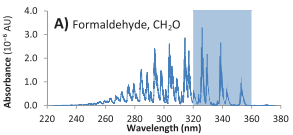
\includegraphics{Figures/HCHO/HCHOAbsorbanceDavenport.png}
      \caption{ HCHO spectrum, with a typical band of wavelengths used for DOAS path measurements.
	This is a portion of an image from \citet{Davenport2015}.}
      \label{ch_LitRev:fig:HCHOSpectrum}
    \end{figure}
    
    
    In MAX-DOAS retrievals, the measurements of light absorption are performed over several elevations in order to add some vertical resolution to the measurement of trace gas concentrations.
    An example of this is shown in figure \ref{ch_LitRev:fig:MAXDOASExample}, which was taken from \citet{Lee2015}.
    Recently MAX-DOAS has been used to examine HCHO profiles in the clean free troposphere \citep{Franco2015, Schreier2016} as well as in polluted city air \citep{Lee2015}.
    Depending on orography and atmospheric composition (ie. the influence of interfering chemicals), MAX-DOAS can be used to split the tropospheric column into two partial columns; giving a small amount of vertical resolution to HCHO measurements \citep[eg.]{Franco2015, Lee2015}.
    
    \begin{figure}
      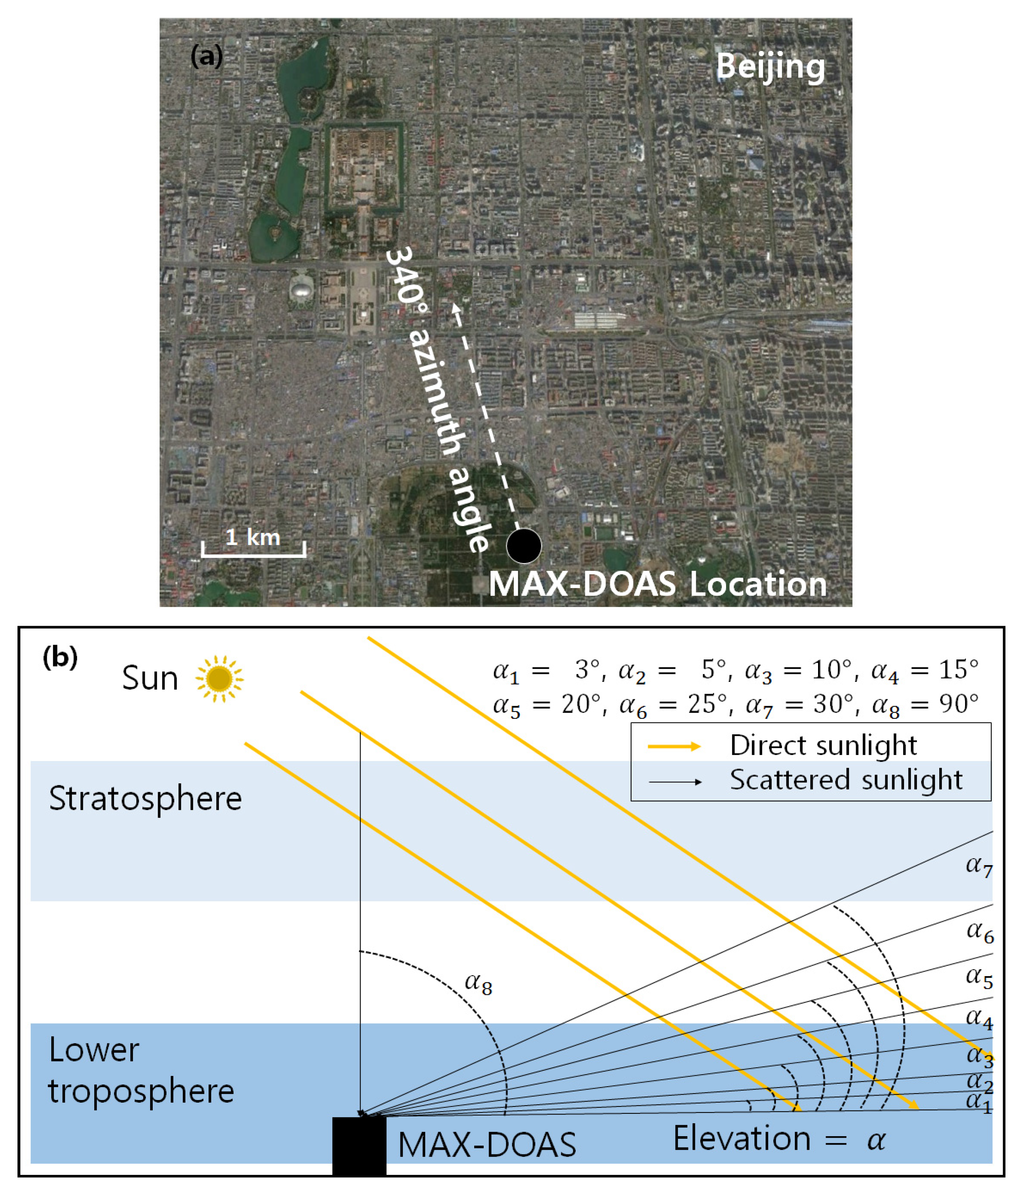
\includegraphics{Figures/MAXDoasExample.png}
      \caption{ %
        Image from \citet{Lee2015}.
      }
      \label{ch_LitRev:fig:MAXDOASExample}
    \end{figure}
    
    Other measurement techniques include chromatographic and fluorimetric methods, both of which differ widely from eachother and the spectroscopic method TODO: read \citep{Hak2005}).
    This resulted in HCHO not having a consistent network for global measurements like those for GHGs or Ozone \citep{FortemsCheiney2012}.
    
  \subsection{Relationship with glyoxyl and isoprene}
    Glyoxyl (CHOCHO) is important to us as it shares many properties with HCHO, and may provide additional information in determining isoprene emissions.
    Glyoxyl is another product of VOC oxidation in the atmosphere, with isoprene being the main source globally.
    Isoprene has been used to estimate isoprene emissions (see section \ref{ch_LitRev:sec:IsopFromHCHO}) but many uncertainties exist.
    One of these uncertainties is the yield of HCHO from isoprene, especially in low NO$_X$ environments.
    Glyoxyl could prove complementary to HCHO in constraining isoprene emissions (TODO: Read and cite Vrekoussis2009,2010, Chan Miller 2014, Alvarado 2014).
    
    Under high NO$_X$ conditions, glyoxyl forms rapidly, similarly to HCHO.
    However, glyoxyl also forms in low NO$_X$ environments both slowly (through isoprene epoxydiols), and rapidly (through di-hydroperoxide dicarbonyl compound photolysation (todo: read abstract and cite crounse(Autoxidation of Organic Compounds in the Atmosphere) 2013).
    This process is similar to the proposed mechanisms for hydroperoxyaldehydes by \citet{Peeters2014} and carbonyl nitrates (todo: read and cite M$\:{u}$ller 2014).
    
  \subsection{Satellite measurements}
    Satellite measurements of HCHO are relatively uncertain, however this can be improved by averaging over larger grid boxes or longer time scales.
    an example of this can be seen in \citet{Dufour2009}, where monthly averaging is used to decrease the measurements uncertainty.
    They examine HCHO in Europe, which is low; near the detection limit of satellite measurements.
    Taking monthly averages allows enough certainty that useful inversions can be determined to estimate the source emissions of HCHO.
    
    In satellite HCHO products, concentrations over the remote pacific ocean are sometimes used to analyse faulty instrument readings.
    This is due to the expected invariance of HCHO over this region.
    For instance GOME (an instrument which measures trace gases on board the ERS-2) corrects for an instrument artifact using modelled HCHO over the remote pacific \citep{Shim2015}.
    OMI HCHO products use a similar technique to account for sensor plate drift and changing bromine sensitivity \citep{Abad2015}
    
    For many places the tropospheric column HCHO measured by satellite is biased low, \citet{Zhu2016} examine six available datasets and show a bias of 20 - 51\% over south east USA when compared against a campaign of aircraft observations (SEAC$^4$RS).
    \citet{DeSmedt2015} also found a low bias from 20 - 40\% when comparing OMI and GOME2 observations against ground based vertical profiles, and \citet{Barkley2013} determine OMI to be 37\% low compared with aircraft measurements over Guyana.
    These bias can be corrected by improving the assumed apriori HCHO profiles which are used to calculate the AMFs of the satellite columns.
    
    The OMI measurements used in this research are recalculated using an updated estimate of HCHO profiles and validated against Wollongong total column measurements. 
    Similar to validation performed by other studies TODO: cite and exemplify a few studies ie: \citet{Zhu2016, Marais2015, Palmer2003} 
    
    Uncertainty in the OMI satellite instrument is calculated by the Smithsonian Astrophysical Observatory (SAO) group using the uncertainty in backscattered radiation retrievals \citep{Abad2015, Abad2016}.
    Another method of calculating the uncertainty is used by the Belgian Institute for Space Aeronomy (BIRA) group, who determine uncertainty from the standard deviation of HCHO over the remote pacific ocean (TODO: use both these methods for HCHO section)\citep{DeSmedt2012, DeSmedt2015}.
    
    GOME suffers from similar uncertainties to OMI, as the same general method of DOAS remote measurements are performed.
    The uncertainty from slant column fitting has been calculated for GOME to be $4\times10^{15}$ molecules cm$^{-2}$ \citep{Chance2000, Millet2006}. 
    The conversion factor for slant to vertical columns (AMF) calculation also suffers from errors; primarily from surface albedo, HCHO vertical profile apriori, aerosol, and cloud influence \citep{Millet2006}. 
    AMF uncertainties for GOME are calculated to be $1$ to $1.3\times10^{15}$ molecules cm$^{-2}$ by \citet{Shim2005}.
%----------------------------------------------------------------------------------------
%	Isoprene Section
%----------------------------------------------------------------------------------------
\section{Isoprene}
\label{ch_LitRev:sec:isoprene}

  \subsection{Basics}
    Isoprene, or 2-methylbuta-1,3-diene, is a Volatile Organic Compound (VOC) and has chemical formula of C$_5$H$_8$. 
    Isoprene effects NO$_X$ and HO$_Y$ cycling, and in the presence of NO$_X$, forms tropospheric ozone and SOAs \citep{Wagner2002, Millet2006}.
    Bottom up inventories of VOCs remain largely uncertain due to extensive extrapolation over plant functional types, changing land cover, and parameterised environmental stressors (todo: read and \citep{Guenther2000}).

  \subsection{Sources and Sinks}
    Methane and isoprene each comprise around a third of the yearly global total emission of VOCs.
    However, methane is relatively long lived (years) and is well mixed in the atmosphere while isoprene levels are very volatile and spatially diverse due to a life time of around an hour.
    Estimates put global isoprene emission at roughly 600 Tg yr$^{-1}$, emitted mostly during the day.
    Major emitters are tropical broadleafs (notably eucalypts), and scrubs \citep{Guenther2006, Arneth2008, Niinemets2010, Monks2015}.
    
    Isoprene has a short lifetime during the day, roughly an hour due to OH oxidation (todo: abstract and cite Atkinson and Arey 2003\citep{AtkinsonArey2003}).
    At night when OH concentrations have dropped, isoprene can remain in the atmosphere to be transported. 
    Typically less than half of this night time isoprene is removed through ozonolysis \citep{AtkinsonArey2003}, however, in polluted areas where high levels of NO$_X$ exist, isoprene is consumed by a different radical.
    During the night time, nitrate radicals (NO$_3$) build up, especially in areas with high NO$_X$ levels.
    In areas with high NO$_X$ levels, greater than 20\% of the isoprene emitted late in the day ends up being oxidised by the NO$_3$ radical over night \citep{Brown2009}.
    So while night time isoprene is not as highly concentrated, is does have varying biogenic and anthropogenic sinks.
    At night isoprene has affects on both NO$_X$ concentrations and ozone levels, and can form harmful SOAs \citep{Brown2009, Mao2013}.
    
    Isoprene oxidation by OH is less well understood in lower concentrations of NO.
    Initially isoprene was thought to be a sink for atmospheric oxidants \citep[eg.]{Guenther2000}.
    It was thought that in low NO environments, like those far from anthropogenic pollution and fires, oxidation of isoprene would create hydroxyhydroperoxides (ISOPOOH) and lead to low concentrations of OH and HO$_2$ (together known as HO$_X$) \citet{Paulot2009b}.
    In \citet{Paulot2009b}, the HO$_X$ levels are shown to be largely unnaffected by isoprene concentrations.
    They show that ISOPOOH is formed in yields $> 70\%$, and MACR and MVK is formed with yields $< 30\%$.
    The formation of MACR and MVK produces some HO$_X$, although not enough to close the gap.
    \citet{Paulot2009b} goes on to suggest (and provide experimental evidence) that dihydroxyperoxides (IEPOX) are formed from oxidation of the ISOPOOH, which form precursors for SOAs as well as closing the HO$_X$ concentration gap.
    They then use GEOS-Chem, modified to include IEPOX formation, to estimate that one third of isoprene peroxy radicals react with HO$_2$, and two thirds react with NO. 
    Their work showed another pathway for isoprene based SOA creation, and additionally estimated $95 \pm 45$~TgC yr$^{-1}$ IEPOX being created in the atmosphere without any inclusion in CTMs at that time.
    In \cite{Crounse2012}, MACR products are examined in various conditions and hydroxy recycling is also observed in low NO conditions. 
    
    Although understanding of OH production/recycling in these low NO conditions has been improved, many observations of OH are still quite under-predicted in models \citep{Mao2012}.
    It was shown in \citet{Mao2012}, for a remote forest in California, that the traditional method of OH measurement may be affected by instrument internally generated OH from VOC oxidation.
    This lends more credence to the current understanding of VOC oxidation as it closed the gap between measurements and model predictions.
  %\subsection{Products from isoprene}
  \subsection{Factors affecting isoprene emissions}
    
    \citet{Marais2014} examine factors affecting isoprene emissions, showing how emissions are sensitive to various environmental factors.
    Their work used MEGAN \citep{Guenther1995} and GEOS-Chem to look at how these factors affect surface ozone and particulate matter in Africa.
    One of the important uncertainties seen in MEGAN within this work is the isoprene emissions due to plant type. 
    Canopy level isoprene measurements are made using relaxed eddy accumulation (REA) at several sites in Africa.
    One plant type near a measurement site emits more than other species and it's actual distribution on a larger scale is completely unknown - leading to possible overestimations in MEGAN.
    
    \citet{Stavrakou2014} examined modelled Asian emissions and altered model parameters for temperature, plant type emission factors, incoming solar radiation (insolation) intensity, land use changes, and palm tree forest expansion.
    Changes were constrained by a network of radiation measurements and some experiments with south east Asian forest emissions - and led to reduction in isoprene emissions by a factor of two over the region.
    The Asian region is also shown to have a strong correlation with the Oceanic Niño Index (ONI), with positive anomalies associated with El Niño.
  
  \subsection{Estimates}
    It used to be thought that anthropogenic and biogenic emissions of VOCs were roughly similar (TODO abstract of \citep{Mueller1992}, and more cites).
    It's now clear that biogenic isoprene emissions are far greater than anthropogenic emissions of VOCs \citep{Guenther2006, Kefauver2014}. 
    The estimates are still fairly uncertain, as global measurements are difficult and regional emissions can be very different. 
    The lack of accuracy in BVOC emissions estimates has a large effect on determining with confidence the sources and distribution of pollutants including ozone and organic aerosols.
    Accuracy in VOC measurements is important: it has been shown that even the diurnal pattern of isoprene emissions has an effect on modelling ground level ozone \citep{Hewitt2011,Fan2004}.
    These uncertainties could explain why models of HCHO over Australia are poor at reproducing satellite measurements \citep{Stavrakou2009}.

    \citet{Guenther2006} estimates that the Australian outback is among the world's strongest isoprene emitters with forests in SE Australia having emission factors greater than 16 mg m$^{-2}$ h$^{-1}$ (see figure \ref{ch_LitRev:fig:meganisoprene}).
    These emissions factor estimates are not well verified as there is little coverage of isoprene (or other BVOC) emissions measurements over Australia.
    However, comprehensive coverage of one high yield (generally) product in the atmosphere over Australia exists in the form of satellite measurements.
    
    It is important to note that many estimates of isoprene emission are based on a few algorithms of isoprene emission which can depend greatly on input parameters \citep{Niinemets2010}.
    \citet{Yue2015} has shown that this is still a problem by looking at land carbon fluxes and modelling the sensitivity to VOC emissions estimates using two independent models of VOC emission.
    One model is photosynthesis based and estimates isoprene emissions using electron transfer energies and leaf physiology \citep{Niinemets1999}, while the other (MEGAN) uses the light and canopy temperature (\citep{Guenther1995} TODO: Arneth et al., 2007; Unger et al., 2013).
    Both are sensitive to light and temperature parameterisations.
    
    
    \begin{figure}
      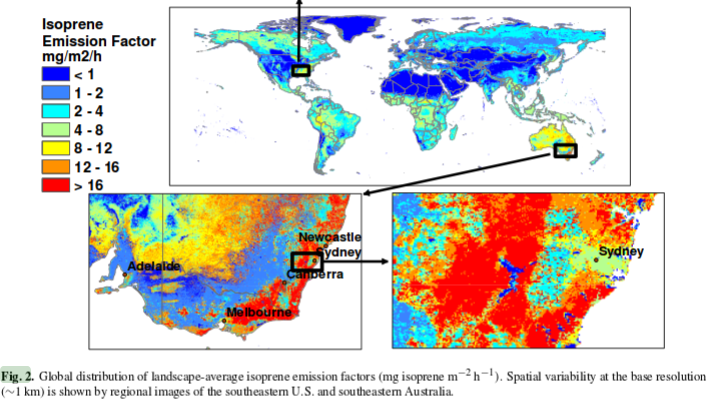
\includegraphics{Figures/MeganIsoprene1.png}
      \caption{ Part of a figure from \citet{Guenther2006} showing global isoprene emission factors. }
      \label{ch_LitRev:fig:meganisoprene}
    \end{figure}
    
  \subsection{Isoprene to HCHO}
    \label{ch_LitRev:sec:IsopFromHCHO}
    In the remote troposphere HCHO production is dominated by methane oxidation, while in the continental boundary layer (CBL) production is largely due to NMVOCs \citep{Abbot2003, Kefauver2014}.
    NMVOCs are alkanes, alkenes, aromatic hydrocarbons and isoprene.
    Isoprene is hard to measure directly due to its short lifetime and weak spectral absorption, instead formaldehyde is often used as a proxy \citep{Millet2006, Dufour2009, Marais2012, bauwens2013satellite, Kefauver2014, Bauwens2016}.
    Formaldehyde formed in the troposphere is mostly due to VOC (roughly one third each: methane, isoprene, others) oxidation.
    We can model this oxidation process in order to work out how much VOC is present based on the total HCHO.
    This requires among other things an idea of which VOCs are present and their yields of HCHO.
    
    The method used to develop top-down isoprene inference using satellites was developed initially by \citet{Palmer2001, Palmer2003}. 
    Isoprene emissions fluxes were derived using the Global Ozone Monitoring Experiment (GOME) satellite instrument.
    Palmer's method improved biogenic isoprene emissions estimates (compared with in-situ measurements) over two available inventories: the U.S. EPA Biogenic Emssions Inventory System (BEIS2) and the Global Emissions Inventory Activity (GEIA).
    This showed an inversion technique which could be used to improve large scale emissions estimates without further expensive measurement campaigns.
    
    \citet{Dufour2009} use HCHO from SCIAMACHY, and examine Europe using CHIMERE as the chemical model. 
    In their work they show that satellite measurements can reduce source emission uncertainty by a factor of two, where emissions are relatively large.
    
    
    Satellites recording reflected solar spectra use Differential Optical Absorption Spectroscopy (DOAS) to measure various trace gases in the atmosphere, including formaldehyde. 
    Formaldehyde levels in the continental boundary layer are generally dominated by chemical formation due to VOC (largely isoprene) emissions \citep{Kefauver2014}.
    
    Satellites can be used to measure the seasonal and interannual variability of HCHO over Australia.
    These records can be compared with modeled estimates of HCHO and used as a proxy to estimate isoprene emissions.
    This has been done in North America \citep{Palmer2003, Millet2006}, South America, Africa, China, Europe \citep{Dufour2009}, and recently globally \citep{FortemsCheiney2012, Bauwens2016}.
    Often these works use two forms of measurement such as satellite and aircraft data combined for validation \citep{Marais2014}.
    
    Initially studies assumed a simple linear steady-state relationship between HCHO and it's precursors \citep{Palmer2003, Palmer2006, Millet2006}.
    This allowed a simple calculation of isoprene using the measured HCHO, with estimated reaction rates and yields.
    The methodology for calculating VOCs from HCHO is laid out in \citet{Palmer2003}, and takes into account the expected lifetime and reaction rates of the precursor VOCs and HCHO.
    Assuming HCHO is produced quickly from short-lived intermediates, and the column is at steady state:
    \begin{eqnarray*}
    VOC_i \overset{k_i}{\rightarrow} Y_i HCHO
    \end{eqnarray*}
    Where $Y_i$ is HCHO yield per C atom (a measure of how much HCHO will form per gram of C from a VOC within a system), and $k_i$ is the reaction rate.
    Then assuming a steady state of atmospheric HCHO ($\Omega$ molecules $cm^{-2}$) produced by oxidation of VOCs (VOC$_i$) and no horizontal transport:
    \begin{eqnarray*}
    \Omega = \frac{1}{k_{HCHO}} \sum_{i} Y_i E_i
    \end{eqnarray*}
    Where i indexes a chemical species, $k_{HCHO}$ is the HCHO loss rate due to OH and photolysis, Y$_i$ is the molar HCHO yield from oxidation of i, and $E_i$ is emission fluxes ( C atoms $cm^{-2}s^{-1}$).
    
    Estimates of Y$_i$ can be attained from a model as shown in \citet{Millet2006}.
    This involves a reduced major axis (RMA) correllation calculation between modelled HCHO and isoprene columns, multiplied by their loss rates (to photolysis and oxidation) (as a normalising factor).  
    In high NOx environments where HCHO has a lifetime on the order of 30 minutes, it can be used to map isoprene emissions with spatial resolution from 10-100 kms.
    Horizontal transport 'smears' the HCHO signal so that source location would need to be calculated using windspeeds and loss rates \citep{Palmer2001,Palmer2003}.
    For more details on this see section \ref{ch_LitRev:sec:smearing}.
    
    Another method of correcting isoprene emissions using observed HCHO total column involves a Bayesian inversion.
    \citet{Shim2005} work with GOME HCHO observations and GEOS-Chem, looking at areas with high signal to noise ratio (higher HCHO concentrations).
    They show that the model underestimates isoprene emissions and HCHO concentrations by 14-46\%, with the corrected VOC emissions reducing the model biases to 3-25\%.
    
    The Bayesian inversion is also used in \citet{Curci2010}, where a regional CTM (CHIMERE) simulates HCHO, which is compared against OMI observed HCHO and shown to be regionally biased.
    This bias is expected to be caused by errors in MEGAN's natural isoprene emissions.
    The CHIMERE model is used to derive yields of HCHO from the various local VOCs and these are then used in estimating local emissions.
    The model is run initially with emissions of BVOCs and reactive anthropogenic VOCs (RAVOCs) turned off in order to work out the background (b) values of these compounds.
    The Bayesian inversion is used to correct regionally biased biogenic isoprene emissions by optimising these parameters in order to simulate HCHO closest to the observed HCHO levels.
    \cite{Curci2010} uses CHIMERE as the forward model to determine the relationship between HCHO (y), isorene and reactive anthropogenic VOCs (\textbf{x}), using 
    \begin{equation}
        y=\mathbf{K}x + b + \epsilon
    \end{equation}
    where $\epsilon$ are the (assumed) independent errors in measurements.
    K is the Jacobian matrix determined from CHIMERE representing the sensitivity of y to the state variable x.
    This K matrix is used in conjunction with error covariance in x to determine the Maximum A Posteriori (MAP) solution to calculate the optimal estimate of x ($\hat{x}$).
    
    TODO: Read through this list of sources on the hcho to isop process : taken from Wolfe2015
    Such techniques have informed isoprene emission inventories in North America (Abbot et al., 2003; Millet et al., 2008 \citep{Palmer2003,Millet2006,Palmer2006}), South America (\citep{Barkley2013}, 2008), Europe \citep{Curci2010,Dufour2009}, Africa \citep{Marais2012}, Asia (Fu et al., 2007; Stavrakou et al., 2014), and globally (Fortems-Cheiney et al., 2012; \citep{Shim2005}; Stavrakou et al., 2009).
    
    More recently, full inversions that better account for transport, source attribution, and chemical schemes have been implemented \citep{FortemsCheiney2012}.
    TODO: full description of this better inversion technique going through FortemsCheiney2012.
  
  \subsection{Smearing}
  \label{ch_LitRev:sec:smearing}
    The distance travelled downwind (L$_{d,i}$ by a precursor (i) before becoming HCHO can be estimated using:
    \begin{equation*}
      L_{d,i} = \frac{U}{k_i - k_{HCHO}} \ln{ \left( \frac{k_i}{k_{HCHO}} \right) }
    \end{equation*}
    where U is windspeed.
    \citet{Palmer2003} further define a smearing length scale: L$_{s,i}$ as the distance downwind where a fraction (1 - $1/e$) of the precursor is completely transformed into HCHO.
    This equation uses the initial VOC column concentration ($[VOC]_0$) at the point of emission and mass balance equations, and is as follows:
    \begin{equation}
      \frac{1}{k_{HCHO}-k_i} \left( k_{HCHO} \exp{ \left[ \frac{-k_i L_{s,i}}{U} \right]} -k_i \exp{ \left[ \frac{-k_{HCHO} L_{s,i}}{U} \right]} \right) = \frac{1}{e} 
    \end{equation}
    with limiting values L$_{s,i} \rightarrow U/k_i$ for $k_i << k_{HCHO}$, and L$_{s,i} \rightarrow U/k_{HCHO}$ for $k_{HCHO} << k_i$.  
    
    Accounting for transport of the precursors is important, especially in low NO$_X$ conditions in which isoprene has a longer lifetime (days).
    This allows horizontal transport to occur and complicates the algorithms, as can be seen by the smearing length scale which increases beyond the 100~km.
    For conditions where VOCs have a lifetime of days determining the major HCHO contributors requires a complex inversion to map HCHO columns to VOC emissions.
    
  \subsection{Measurements}
  
    There are relatively few measurements of isoprene in the southern hemisphere, including MUMBA(TODO CITE), other campaigns?, and very recently that girl from Macquarie University with an instrument in the daintree rainforest(TODO CITE, DESCRIBE?).
    Since 1997, when GOME first measured HCHO over Asia (TODO cite thomas 1998), satellites have been able to provide a total column measurement of one of the primary products of isoprene.
    
    
  \subsection{Estimates}
    There are two commonly used ways of estimating isoprene emissions, top-down or bottom-up.
    Bottom-up emission estimates generally model the flora and events which emit isoprene, like Eucalypts, factories, shrubs, leaf areas under sunlight, etc.
    Understanding how much isoprene is emitted, when and by what is more complicated than it sounds, and since little data exists with which to verify these bottom-up emission inventories they are uncertain on a large scale.
    Top-down estimates look at how much of a chemical is in the atmosphere and try to work out how much of it's major precursors were emitted.
    For isoprene this is done by looking at atmospheric HCHO enhancement, which can be largely attributed to isoprene emissions as long NO$_X$ and transport effects are accounted for.
  
  \subsection{Isoprene products}
    Isoprene forms many products with various lifetimes, here I will present an overview of some important mechanisms which affect oxidation capacity, ozone and aerosol production.
    Isoprene reacts with OH leading to peroxy radical (ISOPO$_2$) formation.
    In the presence of NO$_X$ ISOPO$_2$ forms organic nitrates after reacting with NO.
    These affect levels of both HO$_X$ (H, OH, peroxy radicals) and NO$_X$, acting as a sink (\citet{Mao2013} and references therein).
    
    The first generation of organic nitrates produced by isoprene oxidation range from 7\% to 12\%, shown in laboratory experiments (todo read abstracts and cite papers in the 3rd paragraph of intro to Mao2013),
    A portion of isoprene nitrates are recycled back to NO$_X$, so may serve as a reservoir of nitrogen and allow its transport to the boundary layer of remote regions (TODO: as prior todo).
    
    During the night isoprene is oxidised by NO$_3$ radicals, which joins to one of the double bonds and produces organic nitrates in high yield (65\% to 85\%) \citep{Mao2013}. (todo: read mao2013 para 3 cites for)
    These organic nitrates go on to produce further SOAs \citep{Rollins2009} (todo read Rollins2009).
  
    Todo: More on \citep{Mao2013} ()chemistry mechanism used in GEOS-Chem v9.02)
    For specific information on the isoprene oxidation mechanisms used by GEOS-Chem V10-01 (used in this work), see section \ref{ch_isop:sec:GEOSChemMechanisms}.
  
  \subsection{Radiative Forcing}

    
%----------------------------------------------------------------------------------------
%	SECTION 5
%----------------------------------------------------------------------------------------
\section{Dust}
\label{ch_LitRev:sec:dust}

  Australia is the greatest source of dust in the southern hemisphere producing around 120~Tg yr$^{-1}$ \citep{Li2008}, however model validation and analysis over Australia is relatively scarce with more focus applied to the northern hemisphere \citep{Fairlie2007, Ridley2013}.
  Atmospheric dust has many direct effects including reduced surface insolation, mineral transfer to remote ocean regions, and health degradation in populated areas \citep{Shao2007}.
  Direct and indirect effects of dust have many implications which are not fully understood, with many models still struggling to explain the atmospheric cycling of dust at larger scales \citep{Rotstayn2011}.

  Australian dust emissions involve various weather conditions, convolving the ENSO cycle with flooding, droughts, and winds.
  Rivers and rain build up the particulate matter in many areas, these are referred to as fluvial deposits.
  Fluvial deposits in the Eyre basin increase the dust base load, which will only have mobility during suitable dry weather conditions.
  These deposits are saltated (loosened from the surface) and transported by strong winds\citep{Zender2003}.

  Synoptic scale measurements of dust concentrations in Australia are made by the Bureau of Meteorology (BOM) and can be used to estimate dust transport caused by large storms. 
  Single storms have been estimated to move up to 2.5 Tg of dust off shore in a single day.
  Yearly dust emissions in Australia are somewhere between 10 and 110 Tg yr$^{-1}$.
  These estimates exemplify the large variability in Australian annual dust transport.

  Dust plays a large role in the oceanic carbon cycle, as dust is a major source of oceanic iron (Fe) deposition.
  Some regions in the ocean are high in nutrients, but low in chlorophyll (HNLC), due to a lack of Fe.
  Oceanic carbon cycling is a complex system in which Fe is a limiting factor, required by plankton in order to fix atmospheric nitrogen into a more bioavailable form such as ammonia.
  Atmospheric deposition into the oceans is a very poorly constrained variable in global models \citep{Grand2015}.
  Model estimates of trace element oceanic deposition are required to quantify the atmospheric impact due to a dearth of in situ measurements in remote open ocean regions.

  Measurements of dissolved iron (DFe) at very low concentrations like those found in surface ocean waters are very easily contaminated, which has contributed the the fragmentary and scarce nature of DFe ocean data sets \citep{Rijkenberg2014}.
  Recent analysis of the US Climate Variability and Predictability (CLIVAR)-CO$_{2}$ Repeat Hydrography Program predicted total deposition flux with uncertainty at a factor of 3.5 \citep{Grand2015}.
  Some headway has been made with the recent GEOTRACES program which has several transects of the major oceans and measures trace elements over multiple depths including Al, Ba, Cu, Cd, Fe, Mn, Ni, Pb, and Zn.
    
  Total iron (TFe) emissions from dust and combustion sources are estimated (by average of several global models) at approximately 35~Tg yr$^{-1}$ and 2 Tg yr$^{-1}$ respectively. A two fold increase in Fe dissolution may have occurred since 1850 due to increased anthropogenic emissions and atmospheric acidity.
  This increase may revert by 2100 due to the affects of emission regulations \citep{Myriokefalitakis2015}.
  Dust, TFe and DFe have strong temporally and spatial variability, with changes having most impact upon HnLC regions.

  Another environmental impact of dust is its contribution to fine particulate matter in the atmosphere.
  Several studies have shown that long term exposure to fine particulate matter (PM2.5) increases mortality. 
  Estimates of yearly premature deaths related to PM2.5 are $\sim$ 2-3 million \citep{Hoek2013, Krewski2009, Silva2013, Lelieveld2015}.   
  These estimates are made using global atmospheric models or model ensembles to quantify population exposure before applying epidemiological models to estimate the increased death rates.
  The main source of uncertainty in premature death rates arises from the difference and uncertainties between and within the atmospheric models.

  Dust affects global climate change through direct radiative forcing.
  Uncertainties in the atmospheric dust concentrations make accurate determination of radiative forcing from other sources more difficult \citep{IPCC_2013_chap8}.


%----------------------------------------------------------------------------------------
%	SECTION 6
%----------------------------------------------------------------------------------------
\section{Models}
\label{ch_LitRev:sec:models}

  \subsection{Chemical Transport Models}
  
    Chemical Transport Models (CTMs) simulate production, loss, and transport of chemical species.
    This is generally calculated using one or both of the Eulerian (box) or Lagrangian (puff) frames of reference.
    CTMs normally solve the continuity equations simultaneously with chemical production and loss for chemicals under inspection. 
    The continuity equations describe transport of a conserved quantity such as mass, which, solved together with production and loss of a chemical forms the basis for a CTM.
    This basis enables a record of the chemical densities and transport over time as a model runs.
    The general continuity equation links a quantity of a substance (q) to the field in which it flows and can be described by the formula:
    \begin{eqnarray*}
	\frac{\partial \rho}{\partial t} + \nabla \cdot j &=& \sigma 
    \end{eqnarray*}
    where $\rho$ is density of q in the field, t is time, $\nabla$ is divergence, j is the flux (the amount of q per unit area per unit time entering or leaving the field), and $\sigma$ is the generation of q per unit volume per unit time.
    Note that $\sigma$ can be positive or negative due to sources and sinks.

    The type of model best suited to modelling the entire earth uses the Eulerian frame of reference, where the atmosphere is broken up into 3-D boxes with densities and transport calculated and stored for arbitrary sequential steps in time at each location.
    The mass balance equation must be satisfied in any realistic long term box model and is as follows: 
    \begin{align*}
	\frac{dm}{dt} &=& \sum{sources}-\sum{sinks} \\
	&=& F_{in} + E + P - F_{out} - L - D 
    \end{align*}
    where m is mass of a chemical, E and D are emission and deposition, P and L are production and loss, and F is chemical transport in and out, as shown in figure \ref{ch_LitRev:fig:boxmodel}.
    Many chemical species interact with each other through production and loss. 
    Any large chemical model will solve this mass balance equation over highly coupled arrays of partial differential equations which can be complex and time consuming.

    In many CTMs the isoprene emissions are calculated elsewhere with their own models (EG: \citet{Guenther2006}).
    These estimates can then be used as boundary conditions.
    Trace gases with short lifetimes and complex chemistry such as isoprene are often hard to measure which makes verifying model estimates difficult.

    \begin{figure}
      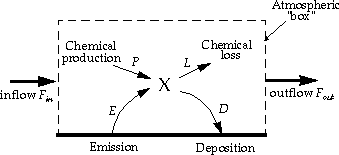
\includegraphics{Figures/boxmodel.png}
      \caption{ Standard box model parameters, image taken from \citet{Jacob_1999_book}. }
      \label{ch_LitRev:fig:boxmodel}
    \end{figure}

  \subsection{GEOS-Chem}
  
    GEOS-Chem is a well supported global, Eulerian CTM with a state of the science chemical mechanism, with transport driven by meteorological input from the Goddard Earth Observing System (GEOS) of the NASA Global Modeling and Assimilation Office (GMAO).
    GEOS-Chem simulates more than 100 chemical species from the earth's surface up to the edge of space (0.01 hPa) and can be used in combination with remote and in-situ sensing data to give a verifiable estimate of atmospheric gases and aerosols.
    It was developed, and is maintained, by Harvard University staff as well as users and researchers worldwide. 
    Several driving meteorological fields exist with different resolutions, the finest at 0.25 by 0.3125$^\circ$ horizontally at 5 minute time steps with 72 vertical levels.
    
   GEOS-Chem has boundary conditions based on several meteorological and emissions inventories, the following are the versions of theses used by GEOS-Chem v 10.01. 
   Meteorological fields can be driven by NASA's GEOS-5 data (0.5$^{\circ}$ x 0.666$^{\circ}$) (TODO:Chen et al., 2009), which exists up to 2013, or GEOS-FP data (0.25$^{\circ}$ x 0.3125$^{\circ}$).
   Fire emissions come from the GFED4 product \citep{Giglio2013}. Anthropogenic VOC emissions come from the EDGAR inventory, while biogenic VOC emissions are coupled to the MEGAN model TODO:cites.

    Combining satellite data with model outcomes provides a platform for the understanding of natural processes to be tested now and into the future over Australia and anywhere with few in-situ measurements.
    Due to the low availability of in-situ data covering most of the Australian continent, a combination of the models with satellite data may provide improved understanding of emissions from Australian landscapes.
    Improved emissions estimates will in turn improve the accuracy of CTMs, providing better predictions of atmospheric composition and its response to ongoing environmental change.

%----------------------------------------------------------------------------------------
%	SECTION 7
%----------------------------------------------------------------------------------------
\section{Satellites}
\label{ch_LitRev:sec:satellites}

  \subsection{Useful satellites}
    Several satellites provide long term trace gas observations with near complete global coverage, including the ERS-2 launched in April 1995 which houses the GOME ultraviolet and visible (UV-Vis) spectrometer, the AURA launched in July 2004 which houses the OMI UV-Vis spectrometer, the MetOp-A and B launched in October 2006 and September 2012 respectively both housing a GOME-2 UV-Vis spectrometer.
    These satellites are on Low Earth Orbit (LEO) trajectories and overpass any area up to once per day. 
    They record near nadir (nearly vertical) reflected spectra between around 250-700~nm split into spectral components at around $0.3$~nm in order to calculate trace gases including O$_3$, NO$_2$, and HCHO.
    An example of a spectrum retrieved from the GOME-2 instrument is given in figure \ref{ch_LitRev:fig:gomeproducts}.

    \begin{figure}
      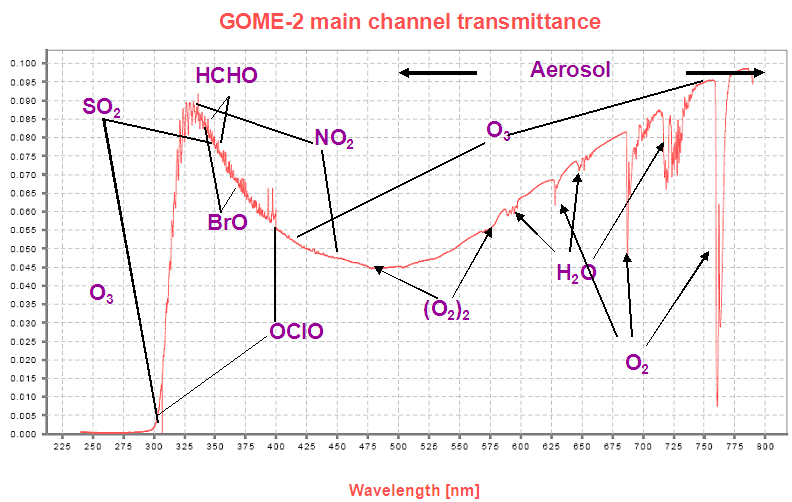
\includegraphics[width=\textwidth]{Figures/GOME_SPECTRUM.jpg}
      \caption{An example spectrum showing interferences used for species concentration measurements by GOME-2. Image by EUMETSAT and ESA \citep{GOME2Image}.}
      \label{ch_LitRev:fig:gomeproducts}
    \end{figure}

    
    Formaldehyde (HCHO) is often used as a proxy to estimate isoprene emissions \citep{Marais2012,bauwens2013satellite}.
    Satellites can use DOAS techniques with radiative transfer calculations on solar radiation absorption spectra to measure column HCHO (eg: \citet{Leue2001}).
    Several public data servers are available which include products from the satellites just mentioned, including NASA's Mirador (http://mirador.gsfc.nasa.gov/) and the Belgian Institute for Space Aeronomy (IASB-BIRA) Aeronomie site (http://h2co.aeronomie.be/).

    Instruments including MODIS on board the AQUA and TERRA satellites are able to determine aerosol optical depth (AOD), a measure of atmospheric scatter and absorbance. 
    An AOD of under 0.05 indicates a clear sky, while values of 1 or greater indicate increasingly hazy conditions.
    This is an important atmospheric property allowing us to track dust storms and pollution events as well as determine where measurements from other instruments may be compromised by high interference.
    Satellite measured AOD requires validation by more accurate ground based instruments like those of AERONET which uses more than 200 sun photometers scattered globally. 
  
  \subsection{Comparisons with Models}
  
    DOAS methods can be heavily influenced by the initial estimates of a trace gas profile (the apriori) which is often produced by modelling, so when comparing models of these trace gases to satellite measurements extra care needs to be taken to avoid introducing bias from unrealistic a priori assumptions.
    One way to remove these apriori influences is through the satellite's averaging kernal, which takes into account the vertical profile of the modelled trace gas and instrument sensitivity to the trace gas \citep{Eskes2003, Palmer2001}.
    Measurements done using DOAS often apply a forward radiative transfer model (RTM) such as LIDORT in order to determine a trace gas's radiative properties at various altitudes.
  
  \subsection{DOAS}
    TODO: some of this is repeated in isoprene chapter satellite section.
    
    The DOAS technique uses solar radiation absorption spectra to measure trace gases through paths of light.
    The RTM used in DOAS techniques is based on Beer's law relating the attenuation of light to the properties of the medium it travels through.
    Beer's law states that $ T = I/I_0 = e^{-\tau} $ with T being transmittance, $\tau$ being optical depth, and I, I$_0$ being radiant flux received at instrument and emitted at source respectively.
    Using 
    $ \tau_i = \int \rho_i \beta_i ds $ gives us:
    $$ I = I_0 \exp {\left( \Sigma_i \int \rho_i \beta_i ds \right) } $$
    Where i represents a chemical species index, $\rho$ is a species density(molecules per cm$^3$), $\beta$ is the scattering and absorption cross section area (cm$^2$), and the integral over ds represents integration over the path from light source to instrument.
    The forward RTM used for satellite data products also involves functions representing extinction from Mie and Rayleigh scattering, and the efficiency of these on intensities from the trace gas under inspection, as well as accounting for various atmospheric parameters which may or may not be estimated (e.g. albedo).
    
    To convert the trace gas profile from a reflected solar radiance column (slanted along the light path) into a purely vertical column requires calculations of an air mass factor (AMF).
    In satellite data, the AMF is typically a scalar value for each horizontal grid point which will equal the ratio of the total vertical column density to the total slant column density. This value should also account for instrument sensitivities to various wavelengths at various altitudes, and is unique for each trace gas under consideration.
  

    %% CHAPTER 2 (probably)
%% MODELLING and DATA

\chapter{Data and Modelling} %with GEOS-Chem} % Main chapter title
\label{Model} %better reference name?
  
\section{Introduction}
  %Why use models?
  % Models
  
  In this thesis the word model is most often used to represent a chemical transport model (CTM), which simulates chemistry and chemical transport through the atmosphere.
  Models of the atmosphere can be used to improve measurements, estimate concentrations in regions not sampled, and allow predictions of atmospheric composition in the future.
  Models of ozone in the atmosphere are used broadly for international assessments of ozone related emissions and processes which involve ozone (such as radiation) \parencite{Young2018}.
  %\textcite{Young2018} summarise current global ozone modelling standards and the metrics and processes used to evaluate these models.
  Models can provide an estimate of trace gas concentrations without requiring measurements, however verification is required.
  
  
  In-situ measurements from campaigns or measurement stations can be used to examine what is happening at a particular (or several) location(s).
  These data are useful to determine how accurate models or estimates are - however the utility is limited to where the measurements have been made.
  In this thesis data from several campaigns are compared against model outputs.
  
  %Satellite usage and reduction of uncertainty
  Satellite datasets give us access to lots of data over large areas.
  However, satellite measurements can have high amounts of uncertainty due to instrument limitations.
  Many datapoints can be averaged in order to reduce uncertainty.
  In this thesis several satellite datasets are combined to provide biogenic HCHO amounts over Australia.
  In order to compare satellite data with other datasets, some work must be undertaken to avoid introducing bias \parencite[eg.][]{Palmer2001, Eskes2003, Marais2012, Lamsal2014}.
  
  In this chapter, modelled data are compared against both campaign measurements and satellite data in order to analyse Australia specific HCHO and isoprene sensitivities and to determine where the GEOS-Chem model needs the most improvement.
  Section \ref{Model:Datasets} lists and describes the campaign datasets, section \ref{Model:GC} describes the GEOS-Chem model, the creation and effects of filters are described in section \ref{Model:Filter} TODO: rest of section outlined.

\section{Measurement Techniques}
  \label{Model:Meas}
  While I have not made any measurements myself, it is important to understand the techniques used in datasets I have utilised in order to understand possible anomalous datapoints or trends.
  % Measurement difficulties
  In-situ measurements contain errors, and depending on the device used and chemical being measured this error can be significant.
  The major sources of uncertainty in measurement techniques included interference from non-target compounds and under-reporting \parencite[eg.][]{Dunne2017}.
  Overall isoprene uncertainty in measurements analysed by \textcite{Dunne2017} was a factor of 1.5 to 2.
  This can feed into uncertainties in modelling and satellite retrievals, as verification and correlations are affected.
  
  \subsection{DOAS}
    \label{Model:Meas:DOAS}
    
    The DOAS technique uses solar radiation absorption spectra to measure trace gases through paths of light.
    % Beer lambert
    Beer's law states
    \begin{equation} \label{Model:Meas:DOAS:eqn_beerslaw}
    T = I/I_0 = e^{-\tau}
    \end{equation}
    with T being transmittance, $\tau$ being optical depth, and I, I$_0$ being radiant flux received at instrument and emitted at source respectively.
    The Beer-Lambert law of extinction allows spectroscopic measurement of absorbing chemical species (absorbers) in the atmosphere:
    \begin{equation} \label{Model:Meas:DOAS:eqn_backscatterextinction}
    I_B = I_{B_0} e^{-\tau_s}
    \end{equation}
    where I$_B$, I$_{B_0}$ is backscattered intensity with and without the absorber respectively, and $\tau_s$ is the optical thickness of the absorber along the measured path between source and instrument.
    
    $\tau$ can be described using the scattering and absorption cross section area ($\alpha$, cm$^{2}$) and density ($\eta$, molec cm$^{-3}$) of an absorber as follows:
    \begin{equation} \label{Model:Meas:DOAS:eqn_tau}
    \tau = \int \alpha(s) \eta(s) \mathrm{d}s
    \end{equation}
    $\tau$ through a medium is the sum of optical thicknesses of each absorber within the measured path, and subbing \ref{Model:Meas:DOAS:eqn_tau} into \ref{Model:Meas:DOAS:eqn_backscatterextinction} leads to
    \begin{equation*}
    I = I_0 \exp { \left( \Sigma_i \int \eta_i \alpha_i ds \right) }
    \end{equation*}
    Where i represents a chemical species index, and the integral over ds represents integration over the path from light source to instrument.
    
    % Optical depth through the atmosphere
    Another way of describing optical depth (also called optical thickness) is the natural logarithm of the ratio of incident radiant power to transmitted radiant power through a material (from equation \ref{Model:Meas:DOAS:eqn_backscatterextinction}).
    In the atmosphere we are interested in the optical depth of various chemical species, and we use incoming solar radiation to determine this.
    The difference between solar radiation at the top of the atmosphere and the Earth's surface defines the atmospheric optical depth along the path of observation.
    \begin{equation*}
    \tau = \ln{\frac{\phi_e^i}{\phi_e^t}}
    \end{equation*}
    where $\phi_e^i$ is radiant flux seen at the earth surface, $\phi_e^t$ is the solar radiant flux which arrives at the top of the atmosphere.
    In the atmosphere, optical depth can be due to several factors including scattering, chemical absorbance, and aerosols.
  
  \subsection{Satellites}
    \label{Model:Meas:sat}
    
    % Satellites use DOAS for trace gases which we are interested in, which includes 
    In order to detect trace gases such as HCHO, satellites use a DOAS based technique to detect concentrations along the path of light which reaches the satellite instrument.
    This requires chemical transport and radiative transfer models used to transform the non-vertical light path into vertical column amounts.
    Measurements done using DOAS often apply a forward radiative transfer model (RTM) such as LIDORT (see section \ref{Model:Meas:sat:LIDORT}) in order to determine a trace gas's radiative properties at various altitudes.
    The forward RTM used for satellite data products also involves functions representing extinction from Mie and Rayleigh scattering, and the efficiency of these on intensities from the trace gas under inspection, as well as accounting for (often estimated) atmospheric parameters such as albedo.
    
    In the absence of atmospheric scattering a simple geometric AMF can be defined as a function of the solar zenith angle. 
    The solar zenith angle ($\theta_s$) and the satellite viewing angle ($\theta_v$) are shown in image \ref{ch_HCHO:fig:zenithangle}.
    However, in the UV-VIS region of the spectrum, Rayleigh and Mie scattering (see section \ref{Model:Meas:DOAS}) must be accounted for.
    
    
    \begin{figure}\begin{center}
      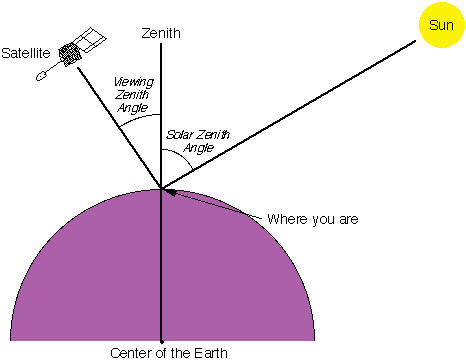
\includegraphics[width=0.6\textwidth]{Figures/ZenithAngles.png}
      \caption{Solar and viewing zenith angles, image copied from \textcite{SZA_Image}, originally from a NASA website.}
      \label{ch_HCHO:fig:zenithangle}
    \end{center}\end{figure}
    
    Rayleigh and Mie scattering describe two kinds of particle effects on radiation passing through a medium.
    Rayleigh scattering is heavily wavelength dependent, and is the dominant form of scattering from particles up to roughly one tenth of the wavelength of the scattered light.
    Mie scattering is more generally involves larger particles, and has less wavelength dependence.
    %These scattering functions are described in detail at (maybe TODO:section? reference?).
    The effects of scattering are what gives us the information about substances in the atmosphere.
    The different particles and gases in the air have various properties which affect remote sensing devices such as a satellite, making them more or less sensitive at certain altitudes for detecting various species \parencite[e.g.][]{Martin2002}.
    
    Satellites record near nadir (vertical) reflected spectra between around 250-700~nm split into spectral components at around $0.3$~nm in order to calculate trace gases including O$_3$, NO$_2$, and HCHO (eg: \textcite{Leue2001}).
    Satellite measurements are generally performed using spectral fitting followed by conversion to vertical column densities.
    %The use of multiple satellites can even be used to detect intradiel concentrations in trace gas columns, as shown in \textcite{Stavrakou2015} using OMI and GOME-2 measurements, which have respective overpass times of 1330 and 0930 LT.
    Several public data servers are available which include products from satellites, including NASAs Earthdata portal (\url{https://earthdata.nasa.gov/}) and the Belgian Institute for Space Aeronomy (IASB-BIRA) Aeronomie site (\url{http://h2co.aeronomie.be/}).
    
    
    Difficulties can arise when aerosols interfere with recorded spectra (eg. clouds, smoke, dust), however some of these can be detected and filtered out.
    Instruments including MODIS on board the AQUA and TERRA satellites are able to determine aerosol optical depth (AOD), a measure of atmospheric scatter and absorbance. 
    An AOD of under 0.05 indicates a clear sky, while values of 1 or greater indicate increasingly hazy conditions.
    This is important in order to determine where measurements from other instruments may be compromised by high interference.
    Satellite measured AOD requires validation by more accurate ground based instruments like those of AERONET which uses more than 200 sun photometers scattered globally.
    
    Soon even more HCHO data will be available in the form of geostationary satellite measurements (\textcite{Kwon2017}).
    \textcite{Kwon2017} examine simulated geostationary measurements against GEOS-Chem column simulations to determine the most important instrument sensitivities.
    Geostationary satellites can provide temporally rich measurements over an area, as they are not sweeping around the earth but fixed relative to one latitude and longitude.
  
  \subsubsection{LIDORT}
  \label{Model:Meas:sat:LIDORT}
  
    %http://www.rtslidort.com/about_publications.html
    LIDORT is a model of LInearized Discrete Ordinate Radiative Transfer, used to determine backscatter intensities and weighting functions at arbitrary elevation angles \parencite{Spurr2001}.
    The model solves radiative transfer equations and can be used to determine various atmospheric column measurement attributes such as optical depth, ring effects, and scattering.
    These radiative properties (or at least estimates thereof) are required when measuring trace gases in the atmosphere through a long path such as seen by satellites \parencite[eg.][]{Palmer2001,Martin2002a,DeSmedt2015,Abad2015}.
  
  
  
  \subsubsection{OMI}
  
    The OMI instrument on board AURA has been active since July 2005, it records spectra from 264-504~nm using an array of 60 detectors with mid-resolution (0.4-0.6~nm).
    This band of wavelengths allows measurments of trace gases including O$_3$, NO$_2$, SO$_2$, HCHO, and various other quantities like surface UV radiation.
    Recently \textcite{Schenkeveld2017} analysed the performance over time of the instrument and found irradiance degradation of 3-8\%, changed radiances of 1-2\%, and a stable wavelength calibration within 0.005-0.020~nm.
    They also provide a very nice summary of the OMI instrument copied here in Fig. \ref{LR:HCHO:Sat:fig_Shenkeveld_OMI_summary}, as it shows the instruments spectral, temporal, and spatial resolutions.
    These changes are measured excluding the row anomaly (RA) effect, which is relatively stable since 2011, although it is still growing and remains the most serious concern.
    An analysis of the row anomaly by \textcite{Huang2017} state that OMI ozone columns remain suitable for scientific use, with recommendation for further evaluation.
    And analysis of OMI output by \textcite{Schenkeveld2017} concludes that data is still of high quality and will deliver useful information for 5-10 more years, with radiances only changing by $1-2\%$ outside of RA impacted areas.
    The RA began in June 2007, with some cross-track rows seemingly blocked. The most likely cause is some instrument insulation partially obscuring the radiance port (\textcite{Schenkeveld2017}).
    
    \begin{figure}
      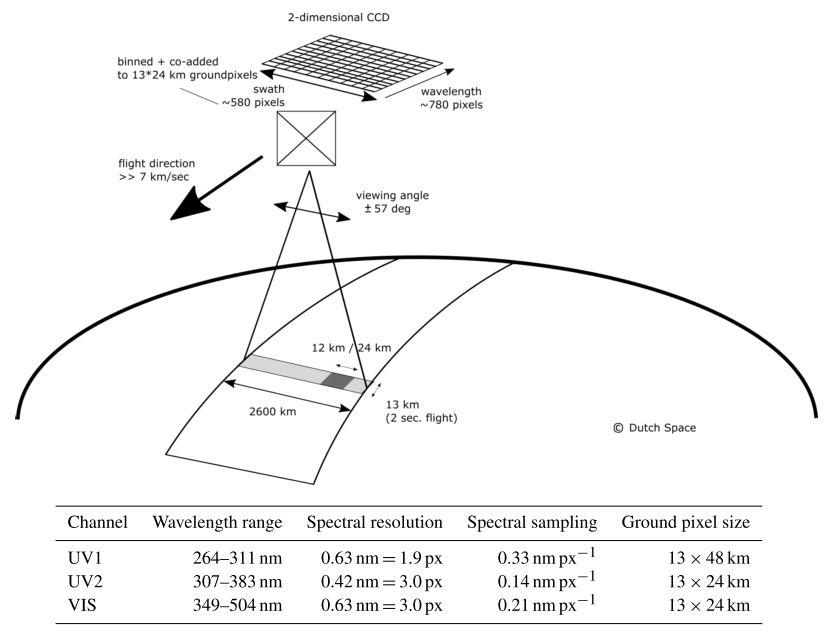
\includegraphics[width=\textwidth]{Figures/Shenkeveld_OMI_summary.png}
      \caption{ %
        Figure 1 and Table 1 from \textcite{Schenkeveld2017}, with the following caption ``An impression of OMI flying over the Earth.
        The spectrum of a ground pixel is projected on the wavelength dimension of the charge-coupled device (CCD; the columns). 
        The cross-track ground pixels are projected on the swath dimension of the CCD (the rows).
        The forward speed of 7~kms$^{-1}$ and an exposure time of 2~s lead to a ground pixel size of 13~km in the flight direction.
        The viewing angle of 114\degr leads to a swath width on the ground of 2600~km.''
        The table shows the optical properties for OMIs three channels.}
      \label{LR:HCHO:Sat:fig_Shenkeveld_OMI_summary}
    \end{figure}
  
  \subsubsection{Air mass factor (AMF)}
  
    % what satellite amfs are, and what they do
    An AMF characterises measurement sensitivity to a trace gas at various altitudes \cite[e.g.]{Palmer2001}.
    \textcite{Lorente2017} show that AMF calculations can be the largest source of unertainty in satellite measurements.
    Another way of describing AMFs are as measures of how radiance at the top of the atmosphere (TOA) changes with trace gas optical depths at specific altitudes (\textcite{Lorente2017}).
    Calculation of the AMF is important as it is multiplied against the estimated slant columns in order to give vertical column amounts.
    To convert the trace gas profile from a reflected solar radiance column (slanted along the light path) into a purely vertical column requires calculations of an air mass factor (AMF).
    In satellite data, the AMF is typically a scalar value for each horizontal grid point which will equal the ratio of the total vertical column density to the total slant column density.
    This value requires calculations to account for instrument sensitivities to various wavelengths over resolved altitudes, and is unique for each trace gas under consideration.
    
    %how do we get an AMF?
    DOAS retrieval columns are an integration of a trace gas over the instruments viewing path, in order to convert this total to a vertically distributed column a few assumptions and estimates are required. 
    The vertical profile of a trace gas is assumed or estimated via a CTM, while its' scattering and radiative properties are calculated at all altitudes using an RTM. 
    These properties are combined into a single array called the AMF.
    Two examples of this are GOME-2 products on the MetOp-A satellite (\url{http://atmos.caf.dlr.de/gome/product_hcho.html}) and OMI products which use IMAGESv2 combined with LIDORT and GEOS-Chem with LIDORT for product processing respectively \parencite{Chance2002, Abad2015}.
    AMFs are unique to each trace gas and due to their complexity and the influence of cloud cover they remain one of the larger error sources in remote sensing of BVOCs \parencite{Palmer2001,Millet2006}).
    
    % averaging kernal relation to amf, why amfs are important when comparing data
    Related to the AMF is the averaging kernal (AK), which is used to handle instrument measurements which are sensitive to concentrations at different altitudes in the atmosphere.
    DOAS methods can be heavily influenced by the initial estimates of a trace gas profile (the a priori) which is often produced by modelling, so when comparing models of these trace gases to satellite measurements extra care needs to be taken to avoid introducing bias from differing a priori assumptions.
    One way to remove these a priori influences is through the satellites AK (or by using AMFs), which takes into account the vertical profile of the modelled trace gas and instrument sensitivity to the trace gas (\textcite{Eskes2003, Palmer2001}).
    % TODO read and note this paper:
    \textcite{Lamsal2014} recommends that when comparing satellite data to models, the AMF should first be recalculated using the model as an a priori.
    This is in order to remove any a priori bias between model and satellite columns.
    Another way of removing this bias is through deconvolution ($\Omega = AK \times VC_{satellite} + \times (I - AK) VC_{a priori}$) of the averaging kernal (AK) of the satellite instrument.
    The AK represents sensitivities to each species at multiple altitudes through the atmosphere and in the case of OMI, can be approximated from the scattering weights ($\omega(z)$) function as follows:
    \begin{equation} \label{ch_HCHO:eqn:AKfromw}
      AK(z) = \frac{\omega(z)}{AMF}
    \end{equation}
    Note that this is an approximation for the OMI product, which does not include the AK but does include the $\omega$ and AMF, as explained in \textcite{Abad2015}.
    
    % How omi gets its AMF
    The latest OMI algorithm uses a shape factor determined from GEOS-Chem using 47 vertical levels at monthly temporal resolution and 2$^{\circ}$ latitude by 2.5$^{\circ}$ longitude horizontal resolution \parencite{Abad2015}.
    The GEOS-Chem model has been substantially updated since then, and using the more recent version $V10.01$ to recalculate the AMF is performed within this thesis, details are shown in section \ref{Model:omiRecalc}.
  
  \subsubsection{Uncertainties}
    %Satellite Errors
    While satellite data is effective at covering huge areas (the entire earth) it only exists at a particular time of day, is subject to cloud cover, and generally does not have fine horizontal or vertical resolution.
    Concentrations retrieved by satellites have large uncertainties, which arise in the process of transforming spectra to total column measurements, as well as instrument degradation (satellite instruments are hard to tinker with once they are launched).
    Uncertainty in transforming satellite spectra comes from a range of things, including measurement difficulties introduced by clouds, and instrument sensitivity to particular aerosols \parencite{Millet2006}.
    Many products require analysis of cloud and aerosol properties in order to estimate concentration or total column amounts \parencite{Palmer2001,Palmer2003, Marais2012, Vasilkov2017}.
    The main source of error in satellite retrievals of HCHO are due to instrument detection sensitivities, and the vertical multiplication factor \parencite{Millet2006}.
    % amf agreements between groups, but sensitive to a priori
    Calculations of the AMF performed by different groups tend to agree fairly well, as long as all the a priori and ancilliary data is similar.
    Large differences can occur depending on the a priori vertical profile, trace gas concentrations, and cloud properties \parencite{Lorent2017}.
    Choice of RTM and interpolation operations have a relatively small affect compared to the assumed state of the atmosphere, with high structural uncertainty introduced at this stage of AMF calculation - as shown in \textcite{Lorent2017}.
    
    There are two types of measurement error, arguably the worst of these is systematic error (or bias) which normally indicates a problem in calculation or instrumentation.
    If the systematic error is known, it can be corrected for by either offsetting data in the opposite direction, or else fixing the cause.
    A proper fix can only be performed if the sources of error are known and there is a way of correcting or bypassing it.
    Random error is the other type (often reported as some function of a datasets variance, or uncertainty), and this can be reduced through averaging either spatially or temporally. 
    By taking the average of several measurements, any random error can be reduced by a factor of one over the square root of the number of measurements.
    This is done frequently for satellite measurements of trace gases (which are often near to the detection limit over much of the globe).
    For example: \textcite{Vigouroux2009} reduce the measurement uncertainty (in SCIAMACHY HCHO columns) by at least a factor of 4 through averaging daily over roughly 500km around Saint-Denis, and only using days with at least 20 good measurements.
    
    %% grid size and averaging
    Satellite measurements of HCHO are relatively uncertain, however this can be improved by averaging over larger grid boxes or longer time scales.
    An example of this can be seen in \textcite{Dufour2009}, where monthly averaging is used to decrease the measurements uncertainty.
    %They examine HCHO in Europe, which is low; near the detection limit of satellite measurements.
    %Taking monthly averages allows enough certainty that useful inversions can be determined to estimate the source emissions of HCHO.
    The finer nadir resolution of OMI (13 by 24~km${^2}$) compared to other satellites reduces cloud influence \parencite{Millet2006, Millet2008}.
    Although the uncertainty in each pixel is $\sim 2 \times 10^{16}$, which is $5 \times$ higher than GOME, there are $\sim 100-200 \times $ as many measurements due to the smaller footprint and better temporal resolution of OMI, which allows a greater reduction of uncertainty with averaging \parencite{Chance2002,Millet2008}.
    % Uncertainty in OMI pixels measurements
    Uncertainty in a single pixel for OMI is roughly the same magnitude as HCHO background levels.
    The top row in figure \ref{Model:Meas:sat:fig_OMI_uncertainty} shows OMI HCHO columns binned to at 0.25\degr longitude by 0.3125\degr latitude averaged over one day, one month, and one month after filtering.
    Row two shows uncertainty of the satellite data after averaging.
    It's clear that one day of satellite data is too uncertain when binned at 0.25x0.3125\degr horizontal resolution, however after a month with or without filtering the uncertainties become manageable.
    % TODO: Several methods of uncertainty where?
    %There are several methods of calculating this, one of which is used here and compared against the provided uncertainty (TODO) as shown in Section \ref{}.
    If we assume the uncertainty is random error, and not bias introduced through calculation techniques, then we are able to reduce the uncertainty through averaging.
    Random error can be reduced by temporal and/or spatial averaging, decreasing uncertainty by a factor of $1/\sqrt{N}$ where N is the number of observations being averaged.
    High resolution low detection limit estimates can be built up using ``oversampling'', which averages satellite measurements over time \parencite[eg.][]{Zhu2014}.
    %A good example can be seen in \textcite{Zhu2014} where 0.2$^{\circ}$ by 0.2$^{\circ}$ resolution with high enough sensitivity to see anthropogenic HCHO is acheived with three summers worth of satellite data.
    
    % Figure from tests.py
    \mypic{Figures/OMI_link/Uncertainty_OMI_200501.png}{}{\label{Model:Meas:sat:fig_OMI_uncertainty}}
    
    %      \begin{figure}
    %        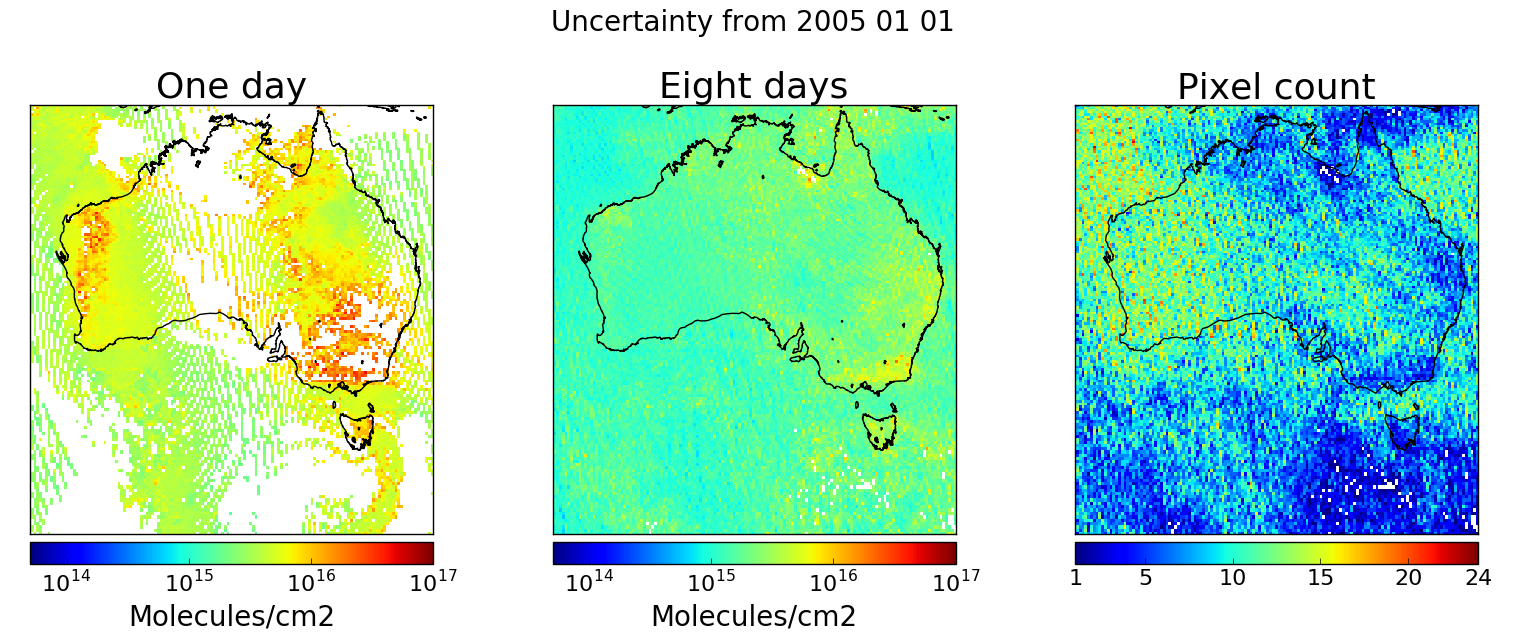
\includegraphics[width=\textwidth]{Figures/HCHO/Uncertainty.png}
    %        \caption{%
    %          OMI uncertainty before and after gridding and averaging 8 days from Jan 1 2005 to Jan 8 2005.
    %          The third panel shows the number of pixels in each grid box after 8 days of averaging, before accounting for fire.
    %        }
    %        \label{Model:Meas:sat:fig_averagingUncertainty}
    %      \end{figure}
    
    %% SURFACE CONDITIONS AND CLOUDS
    In cloudy, hazy or polluted areas measurements are more difficult to analyse (\cite[e.g.][]{Palmer2003,Marais2014}).
    Recent work by \textcite{Vasilkov2017} showed that updating how the surface reflectivity is incorporated into satellite measurements can change the retrievals by 50~\% in polluted areas.
    With the satellite HCHO columns, we filter cloud fractions over 40\%, which introduces a clear-sky bias.
    This bias has been measured as a 13\% positive monthly mean bias by \textcite{Palmer2001, Surl2018}.
    
    %% BACKGROUND MEASUREMENTS
    In satellite HCHO products, concentrations over the remote pacific ocean are sometimes used to analyse faulty instrument readings.
    This is due to the expected invariance of HCHO over this region.
    For instance GOME (an instrument which measures trace gases on board the ERS-2) corrects for an instrument artifact using modelled HCHO over the remote pacific \parencite{Shim2005}.
    OMI HCHO products use a similar technique to account for sensor plate drift and changing bromine sensitivity \parencite{Abad2015}.
    Uncertainty in the OMI satellite instrument is calculated by the Smithsonian Astrophysical Observatory (SAO) group using the uncertainty in backscattered radiation retrievals \parencite{Abad2015, Abad2016}.
    Another method of calculating the uncertainty is used by the Belgian Institute for Space Aeronomy (BIRA) group, who determine uncertainty from the standard deviation of HCHO over the remote pacific ocean \parencite{DeSmedt2012, DeSmedt2015}.
    
    
    %% EXAMPLES OF BIAS
    For many places the tropospheric column HCHO measured by satellite is biased low, \textcite{Zhu2016} examine six available datasets and show a bias of 20 - 51\% over south east USA when compared against a campaign of aircraft observations (SEAC$^4$RS).
    \textcite{DeSmedt2015} also found OMI and GOME2 observations were 20 - 40\% lower than ground based vertical profiles, and \textcite{Barkley2013} determine OMI to be 37\% low compared with aircraft measurements over Guyana.
    These bias can be corrected by improving the assumed a priori HCHO profiles which are used to calculate the AMFs of the satellite columns.
    \textcite{Millet2006} examine OMI HCHO columns over North America and determine overall uncertainty to be 40\%, with most of this coming from cloud interference.
    \textcite{Millet2008} shows that there also exists some latitude based bias, as well as a systematic offset between the OMI and GOME instruments.
    This does not appear to be due to the different overpass times of the two instruments.
    
    %% UNCERTAINTY CALCULATIONS
    
    %A full analysis of the AMF uncertainty in OMI measurements, as well as the structural uncertainty (between different systems of calculations applied to the same data) is performed by \textcite{Lorente2017}.
    AMF calculation uncertainty often dominates the total uncertainty in satellite retrievals, especially in polluted regions \parencite{Lorente2017}.
    In scenarios where the gas is enhanced in the lower troposphere, AMF calculation is the largest uncertainty in satellite measurements.
    In polluted environments the structural uncertainty is estimated at 42~\%, or 31~\% over unpolluted environments \parencite{Lorente2017}.
    Another impact often not included in uncertainty calculations is the structural uncertainty of retrieval methods.
    The structural uncertainty of AMF calculation approaches used by different retrieval groups is the uncertainty due to how the AMF is calculated, rather than uncertainty in the calculation components.
    The importance of a priori and ancillary data (such as surface albedo and cloud top height) sharply affects the structural uncertainty \parencite{Lorente2017}.

\section{Datasets}
\label{Model:Datasets}

  %TODO: Combine these sections
  %\section{Campaigns}
  Here I will describe the various datasets used within this thesis, including modelled output, satellite measurements, and measurement campaigns.
  I will also give details on filtering and groupings which are undertaken when reading data, as each dataset has its own resolution.
  These datasets are used for four purposes: 
  \begin{enumerate}
    \item Model output validation in this chapter
    \item Calculation of biogenic HCHO distribution over Australia in chapter \ref{Model}
    \item Determination of isoprene emissions in chapter \ref{BioIsop}
    \item Extrapolation of ozone transport in chapter \ref{Ozone}
  \end{enumerate}
  

  
  \subsection{Satellite datasets}
    \label{Model:Datasets:Aura}
    
    % Satellite data product levels
    Satellite data products are generally classed into several categories, level 0 through to level 3. Level 0 products are sensor counts and orbital swath data, level 1B data calibrates and geo-locates the level 0 data. 
    Level 2 products additionally have temporal, spatial, solar, and viewing geometry information, as well as quality flags.
    To create level 2 data slant column density is determined and then translated into vertical column density using an AMF calculated through radiative transfer models. 
    Level 3 data is a temporally aggregated version of the this, for instance monthly or yearly averages.
    
    % Aura satellite trace gas measurements
    One satellite is NASA's Earth Observing System's ``Aura'', which provides several useful datasets (products).
    Aura orbits the earth in a polar sun-synchronous pattern, circling the earth on a plane coincident with the sun and the poles.
    % omi instrument on board aura
    Aura houses the Ozone Monitoring Instrument (OMI), a near-UV/Visible Charged Coupled Device (CCD) spectrometer.
    From here on the word pixel is used to describe one data point retrieved by OMI, each pixel includes a latitude and longitude within OMI's data product.
    OMI measures several atmospheric trace gases, including NO$_2$, SO$_2$, BrO, HCHO, O$_3$, and aerosols.
    OMI measurements occur from right to left on a band covering 115$^{\circ}$, resulting in swaths of around 2600~km, with pixel sizes from 13x24~km$^2$ at nadir to 26x135~km$^2$ at the swath edges \parencite{Abad2015}.
    The swaths cover Earth daily, although half of these are at night time and contain no useful near-UV/Visible information.
    OMI spectra are used in several products used in this thesis, including OMNO2d, OMHCHO, and OMAERUVd.
    
    \subsubsection{OMHCHO}
      \label{Model:Datasets:OMHCHO}
      
      % How omhcho is produced
      Atmospheric HCHO can be measured using Differential Optical Absorption Spectroscopy (DOAS), as long as trace gases with similar features near the same wavelength are accounted for.
      A DOAS fit determines the total column amount of a trace gas along the path that the instrument views.
      This uses the Beer-Lambert law where radiance is reduced as light travels through a medium.
      I use the NASA OMHCHOv003 data product \parencite{Abad2015}, with HCHO determined using the spectral window $328.5$~nm$ - 356.5$~nm. 
      The algorithm used is based on direct fitting of radiances, and accounts for competing absorbers, under-sampling, and Ring effects.
      An OMI radiance measurement over the remote Pacific ocean is used instead of an irradiance measurement.
      This means that the slant columns ($\Omega_S$) are actually the difference with respect to the radiance reference column ($\Omega_{S_0}$).
      The full method details for slant column retrieval by OMI are outlined in section \ref{SuppNotes:Satellite:OMI_BOAS}.
      Slant columns range from $\sim 4\times 10^{15} $ to $\sim 6 \times 10^{16}$~molec cm$^{-2}$, with uncertainties from 30\% (larger columns) to over 100\% (smaller columns) \parencite{Abad2015}.
      
      
      % What the swathes look like
      OMHCHO level two data includes 14-15 daily swaths of measurements provided by NASA.
      Each swath contains roughly $9 \times 10^4$ pixels, each of which contains various data including latitude, longitude vertical column HCHO, etc.
      The OMHCHO dataset has a quality flag which can be used to remove unlikely or poor satellite measurements.
      The states represented by this quality flag are shown in table \ref{Model:Datasets:OMHCHO:tab_qflag} which is taken from \textcite{Kurosu2014}.
      Filtering bad or missing measurement pixels is preformed prior to any other filtering, this includes the datapoints affected by the row anomaly.
      This anomaly (\url{http://projects.knmi.nl/omi/research/product/rowanomaly-background.php}) affects radiance data at particular viewing angles, corresponding to a row on the CCD detectors, and is dynamic over time.
      The slant columns affected are flagged and easy to remove before further processing.
      
      \begin{table}
        \caption{OMI quality flag values table from \textcite{Kurosu2014}}
        \begin{tabular}{  l  l  p{10cm} }
          \hline
          \textbf{Value} & \textbf{Classification} & \textbf{Rational} 
          \\ \hline
          0 & Good & Column value present and passes all quality checks; data may be used with confidence. 
          \\ \hline
          1 & Suspect & Caution advised because one or more of the following conditions are present: 
          \begin{itemize}
            \item Fit convergence flag is $<$ 300 but $>$ 0: Convergence at noise level
            \item Column $+ 2 \sigma$ uncertainty $<$ 0 $<$ Column $ + 3 \sigma $ uncertainty
            \item Absolute column value $>$ Maximum column amount (1e19 molec cm$^{-2}$)
          \end{itemize}
          \\ \hline
          2 & Bad & Avoid using as one of the following conditions are present: 
          \begin{itemize}
            \item Fit convergence flag is $<$ 0 : No convergence, abnormal termination
            \item Column $+ 3 \sigma$ uncertainty $<$ 0
          \end{itemize}
          \\ \hline
          $<0$ & Missing & No column values have been computed; entries are missing
          \\ \hline
        \end{tabular}
        \label{Model:Datasets:OMHCHO:tab_qflag}
      \end{table}
      
      % Where does cloud product come from? it removes around 30% of non-qa filtered data
      The cloud fraction with each pixel is provided with the OMHCHO dataset, however its source is the OMI cloud product, OMCLDO2.
      If greater than 40\% of a pixel measurement is cloudy (ie. cloud fraction $>0.4$) then the pixel is removed from subsequent analysis.
      This removes around 30\% of the pixels which remain after filtering out the bad or missing data.
      
      Each $\sim90$ minutes the AURA satellite sweeps over the sunny side of the planet, with OMI recording roughly 90~k pixels, of which around 50~k -- 80~k are classified as good.
      Each pixel contains several important pieces of data which are needed for recalculation of the HCHO vertical column: the total column of HCHO ($\Omega$\moleccm), cloud fraction, associated shape factor, AMF, geometric AMF, scattering weights and their vertical altitudes (hPa), viewing zenith angle, solar zenith angle, latitude, longitude, OMI sensor track, main data quality flag, cross track flag, and total column uncertainty.
      All of these data are needed in order to reconstruct the total vertical column using a modelled a priori shape factor rather than NASA's included a priori shape factor.
      
      Recalculated OMI formaldehyde columns are used as a basis for estimating isoprene emissions in Chapter \ref{BioIsop}.
    
    \subsubsection{OMNO2}
      \label{Model:Datasets:OMNO2d}
      NO$_2$ measured by OMI is used to check whether NO$_2$ is well represented by GEOS-Chem. 
      OMNO2d is a gridded daily level three product with good satellite pixels averaged into 0.25x0.25$^{\circ}$ horizontally resolved bins.
      An example figure from Jan 29, 2005 is shown in figure \ref{Model:Datasets:OMNO2d:fig_eg_omno2d}, while an average for 2005 (global) is shown in figure \ref{Model:Datasets:OMNO2d:fig_omno2d_2005}.
      
      \mypic{Figures/OMNO2d_2005m0129.png}{Example of NO$_2$ tropospheric columns taken from the OMNO2d product.}{\label{Model:Datasets:OMNO2d:fig_eg_omno2d}}
      
      \mypic{Figures/OMNO2d_avg2005.png}
        {Average 2005 tropospheric NO$_2$ from OMNO2d with pixels screened for $<30\%$ cloud cover.}
        {\label{Model:Datasets:OMNO2d:fig_omno2d_2005}}
      
      See section \ref{Model:Analysis:NOx} for the comparison between this product and GEOS-Chem calculations.
    
    
    
    \subsubsection{OMAERUVd}
      \label{Model:Datasets:OMAERUVd}
      
      % smoke aaod outline
      Aerosols in the atmosphere can be seen through their affects on light. 
      Smoke and dust can be seen as an increase in AAOD (see section \ref{Model:Meas:DOAS}).
      This is due these particles scattering and absorbing UV radiation \parencite{Ahn2008}.
      
      
      %TODO: OMAERUVd brief description
      OMAERUVd (DOI: 10.5067/Aura/OMI/DATA3003) provides a useful dataset allowing us to filter gridsquares which may be smoke affected.
      OMI aerosol extinction and absorption optical depths (AOD, AAOD respectively) at three wavelengths (354, 388, and 500~nm), along with UV aerosol index (UVAI), are available publicly from Earthdata: \url{https://disc.gsfc.nasa.gov/datasets/OMAERUVd_V003/summary}.
      The OMAERUVd product is level three, gridded daily data, based on quality filtered level two swath pixels which are then gridded by averaging.
      The product is most sensitive to error in the form of subpixel scale cloud interference, so I select AAOD as the basis for my smoke filter as it is least affected by clouds \parencite{Ahn2008}.
      
      % How I read the AAOD
      Gridded smoke AAOD is read from OMAERUVd at 1x1\degr resolution daily, and mapped to finer resolution using the nearest value for each gridsquare.
      I use the AAOD at 500~nm wavelength, which is blocked by fire smoke plumes.
      This daily AAOD is used to mask fire smoke plume influence, by masking gridsquares with higher AAOD$>0.03$.
    
    \subsubsection{MOD14A1}
      \label{Model:Datasets:MOD14A1}
      Daily gridded fire counts compiled from Terra and Aqua satellite into 1x1~km$^2$ resolution.
      Using this product after binning into a lower resolution allows an active fire influence mask (see section \ref{Model:Filter:fire}).
      
    \subsubsection{AIRS CO columns}
      \label{Model:Datasets:AIRS}
      
      In chapter \ref{Ozone}, potential biomass burning plumes are identified using satellite observations of CO from the AIRS (Atmospheric Infra-red Sounder) instrument aboard the Aqua satellite \parencite{AIRS3STD}.
      
      
  \subsection{Model datasets}
    \subsubsection{Meteorological reanalysis}
      \label{Model:Datasets:ERAI}
      
      Synoptic scale weather patterns are taken from the European Centre for Medium-range Weather Forecasts (ECMWF) Interim Reanalysis (ERA-I) \parencite{Dee2011}.
      These are used in chapter \ref{Ozone} to determine typical weather systems for stratospheric ozone intrusions.
    
  \subsection{Campaign datasets}
    
    %TODO: Add all campaigns to the plot of locations
    In this thesis data from several measurement campaigns are used to examine accuracy of modelled data at specific sites.
    Figure \ref{Model:Datasets:fig_locations} shows the locations of each of the campaigns used in this work.
    These took place over disparate times, and are in-situ measurements which require filtering and interpolation in order to compare against GEOS-Chem output which is averaged over a large horizontal space.
    \mypic{Figures/campaigns/campaign_locations.png}{Locations of Australian campaigns which are analysed within this thesis}{\label{Model:Datasets:fig_locations}}
    
    TODO: these summaries.
    
    \subsubsection{Daintree}
      Daintree summary (P. Nelson)
    
    \subsubsection{Marine and Urban MBA ? (MUMBA)}
      \label{Model:Datasets:MUMBA}
      
      The MUMBA campaign \parencite{PatonWalsh2013} measured various compound abundances including isoprene, formaldehyde, and ozone from 21 December 2012 to 15 February 2013.
      These measurements took place in Wollongong, 10~m above ground level (40~m above sea level).
      Ozone was measured by Thermo UV absorption with 1-minute time resolution averaged into hourly outputs.
      Isoprene and HCHO were measured by Ionicon Proton-Transfer-Reaction Mass spectrometer, with a time resolution of 3-minutes, averaged each hour.
      Detection limits varied due to instrument conditions, and are listed in table \ref{Model:Datasets:MUMBA:tab_detectionlimits}.
      Uncertainty has been estimated to be 15~\%.
      The full dataset has been published on PANGAEA \parencite{Guerette2017}.
    
      \begin{table}
        \caption{Detection limits for MUMBA}
        \begin{tabular}{  l |  l  l  l }
          
          \textbf{Dates} & \textbf{HCHO (ppb)} & \textbf{Isoprene (ppb)} & \textbf{Ozone (ppb)}
          \\ \hline
          21/Dec/2012 - 29/Dec/2012 & 0.205 & 0.003 & 0.5 \\
          29/Dec/2012 - 18/Jan/2013 & 0.105 & 0.005 & 0.5 \\
          19/Jan/2013 - 15/Feb/2013 & 0.186 & 0.003 & 0.5 \\
        \end{tabular}
        \label{Model:Datasets:MUMBA:tab_detectionlimits}
      \end{table}
    
    \subsubsection{Sydney Particle Studies (SPS1, SPS2)}
      \label{Model:Datasets:SPS}
      Two VOC and other trace gas measurement campaigns took place at the Westmead Air Quality Station scientists from CSIRO, OEH, and ANSTO. 
      Stage 1 (SPS1) was from 5 February to 7 March in 2011, while stage 2 (SPS2) ranged from 16 April to 14 May 2012.
      
      Two instruments measured VOC concentrations: one was a Proton transfer reaction mass spectrometer (PTR-MS), the other a gas chromatographer (GC) with an equipped flame ionisation detector (FID).
      The PTR-MS uses chemical ionisation mass spectrometry and can quantify VOCs at high temporal resolution ($< 1$~s).
      It was calibrated several times per day against hcho, isoprene, $\alpha$-pinene, and several more VOCs. Further details can be found in \textcite{Dunne2012, Dunne2018}.
      % Dunne 2018 looks like an analysis of VOC readings from the sites
      The output lists hourly averaged ppbv concentrations of trace gases based on the mass to charge ratio (m/z), which for isoprene is 69.
      
      % Sensitivities
      It's possible that other chemicals (such as Furan, with the same m/z) interfered with this value, especially at low ambient isoprene concentrations and towards the end of autumn (SPS2) when wood fires usage starts to become frequent (TODO cite something).
      The GC-FID analysed samples collected in multi-absorbent tubes, with lower temporal resolution but no interferences. GC-FID data is averaged from 0500-1000~LT, and 1100-1900~LT. Further details for this method can be found in TODO: cite Min et al 2016.
      Uncertainties in VOC measurements range from a factor of 1.5 to 2.
      This includes significant differences between measurement devices when detecting isoprene, potentially due to interfering compounds in the PTR-MS \parencite{Dunne2017}.
      
      Figure \ref{Model:Datasets:SPS:fig_series} shows isoprene and formaldehyde over the course of these two campaigns, as well as the detection limits (dashed lines), as measured by PTR-MS. In order to compare with GEOS-Chem output a daily average and an overpass time (1200-1300 LT) average are both created from these data.
      In averaging, any measurements below the machine detection limit are set to half of the detection limit, as done in \textcite{Lawson2015}. 
      This should minimise any introduced bias.
      
      \mypic{Figures/campaigns/SPS_Series.png}{
        SPS HCHO (yellow) and isoprene (green) time series, along with detection limits (dashed).
        SPS 1 (left) took place in late summer 2011, while SPS 2 (right) occurred during Autumn.
      }
      {\label{Model:Datasets:SPS:fig_series}}
      
      Figure \ref{Model:Datasets:SPS:fig_GC_comparison} shows GEOS-Chem output in the gridsquare containing Sydney overlaid on SPS measurement data.
      Superficially the comparison is not too bad between these two datasets, however GEOS-Chem output is daily averaged over 2x2.5\degr (latitude by longitude)
      The SPS data is point-source and taken during the daytime when isoprene is higher, so it is very likely that GEOS-Chem HCHO and isoprene output is in fact too high.
      
      \mypic{Figures/OMI_link/GC_vs_Campaigns_20050131-20050601.png}{Comparison between GEOS-Chem HCHO concentrations in the gridsquare containing Sydney for the duration of the SPS 1 and 2 campaigns}{\label{Model:Datasets:SPS:fig_GC_comparison}}
      
    \subsubsection{Ozonesondes}
      \label{Model:Datasets:ozonesondes}
      Ozonesonde data comes from the World Ozone and Ultraviolet Data Centre (WOUDC).
    
\section{GEOS-Chem}
  \label{Model:GC}

  \subsection{Overview}
    % Geos chem is a box model with chemistry and meteorology
    GEOS-Chem is a well supported global, Eulerian CTM with a state of the science chemical mechanism, with transport driven by meteorological input from the Goddard Earth Observing System (GEOS) of the NASA Global Modeling and Assimilation Office (GMAO).
    Chemistry, transport, and meteorology are simulated at 15 minute time steps within a global set of 3-D boxes.
    Emissions are either prescribed by inventories or modelled (eg. biogenic emissions are created using the Model of Emissions of Gases and Aerosols from Nature (MEGAN)).
    % It uses GEOS, from GMAO
    
    % This thesis uses 10.01 at 2x2.5 model output
    GEOS-Chem simulates more than 100 chemical species from the earth's surface up to the edge of space (0.01~hPa) and can be used in combination with remote and in-situ sensing data to give a verifiable estimate of atmospheric gases and aerosols.
    It was developed, and is maintained, by Harvard University staff as well as users and researchers worldwide.
    In this thesis I use version 10.01 of GEOS-Chem, which outputs up to 66 chemical species (tracers) in the standard run, at 2 by 2.5$^{\circ}$ horizontal resolution, with 47 levels up to the top of the atmosphere (TOA at 0.01~hPa). 
    
    
    Global CTMs are often run using one or several emission models (or the output from them) to determine boundary conditions for many gridboxes.
    Some of the inventories used by GEOS-Chem are described here.
    Meteorological fields are taken from NASA's GEOS-5 dataset (0.5$^{\circ}$ x 0.666$^{\circ}$) \parencite{Chen2009}, which exists up to April, 2013.
    GEOS-5 meteorological fields are used as the boundary conditions driving transport.
    % Emissions models used for boundary conditions
    Fire emissions come from the GFED4 product \parencite{Giglio2013}. 
    Anthropogenic VOC emissions come from the EDGAR inventory, while biogenic VOC emissions are simulated using the MEGAN model (see section \ref{Model:GC:Isop:MEGAN}).
    MEGAN is used to determine biogenic emissions for our default GEOS-Chem simulation.
    The estimated biogenic VOC emissions are important for accurately simulating chemistry within models, as discussed in Section \ref{LR:Atmos:Chem}.
    
  
  \subsection{Running GEOS-Chem (before isop?)}
    \label{Model:GC:running}
    \subsubsection{Installation and requirements}
      GEOS-Chem instructions for download, compilation, and running can be found in the user guide provided by Harvard: \url{http://acmg.seas.harvard.edu/geos/doc/man/}.
      In order to build and run GEOS-Chem a high-speed computing system is optimal, as globally gridded chemical calculations can take a long time to perform.
      I installed GEOS-Chem onto a suitably configured workspace on the National Computational Infrastructure (NCI, \url{http://nci.org.au/}). 
      This workspace included access to compilers and libraries which are needed to build the Fortran based GEOS-Chem source code, and IDL, Python, and various editors and scripting languages to read, run, edit, and analyse both GEOS-Chem and its output.
      After downloading GEOS-Chem, the code can be compiled with different options for resolution and chemical mechanisms.
  
  \subsection{GEOS-Chem isoprene modelling}
    \label{Model:GC:Isop}

    The isoprene reactions simulated by GEOS-Chem were originally based on \textcite{Horowitz1998}.
    This involved simulating NO$_X$, O$_3$, and NMHC chemistry in the troposphere at continental scale in three dimensions, with detailed NMHC chemistry with isoprene reactions and products.
    The mechanism was subsequently updated by \textcite{Mao2013}, who change the isoprene nitrates yields and add products based on current understanding as laid out in \textcite{Paulot2009a,Paulot2009b}.
    Further mechanistic properties, like isomerisation rates, are based on results from four publications: \parencite{Peeters2009,Peeters2010,Crounse2011,Crounse2012}.
    % Peeters looks at OH adduction and subsequent pathways to reform OH with ~ 80% efficiency overall
    
    
    \textcite{Crounse2011} examines the isomerisations associated with the oxidation of isoprene to six different isomers of ISOPOO formed in the presence of oxygen through $ISOP + OH \to ISOPOO$.
    They determine rates and uncertainties involved in these reactions, and study the rate of formation of C$_5$-hydroperoxyaldehydes (HPALDs) by isomerisation.
    Prior to 2012 oxidation chamber studies were performed in high NO or HO$_2$ concentrations, giving peroxy lifetimes of less than 0.1~s \parencite{Crounse2012}.
    In most environments NO and HO$_2$ concentrations are not so high, GEOS-Chem uses production rates for different NO concentrations and peroxy radical lifetimes determined by \textcite{Crounse2012}.
    OH regeneration through photolysis of hydroperoxy-methyl-butenals (HPALDs, produced by isoprene isomerisation) in areas with high isoprene emissions are included from \textcite{Peeters2010}.
    Photolysis of photolabile peroxy-acid-aldehydes creates OH and improved model aggreement with continental observations.
    OH and HPALD interactions are central to maintaining the OH levels in pristine and moderately polluted environments, which makes isoprene both a source and a sink of OH \parencite{Peeters2010,Taraborrelli2012}.
    
    Formation of isoprene nitrates (ISOPN) have an effect on ozone levels through NO$_X$ sequestration, and the yields and destinies of these nitrates is analysed in \textcite{Paulot2009a}.
    %% ISOPN can be oxidised (by OH) to form nitrated organic products \parencite{Paulot2009a}.
    In a chamber with clean air and high NO concentrations, isoprene photooxidation is initially driven by OH addition, followed by NO$_X$ chemistry (150~min - 600~min), and finally HO$_X$ dominated chemistry.
    GEOS-Chem uses these the yields of various positional isomers of isoprene nitrates, and pathways of their oxidation products, and reactions within its suite of chemical mechanisms determined by \textcite{Paulot2009a,Mao2013}.
    %They use anion chemical ionization mass spectrometry (CIMS) to determine products of isoprene photooxidation.
    
    % First steps in GC: LOW NOx
    In low NO$_X$ ISOPOO reacts with HO$_2$ ($70\%$ yield of hydroxy hydroperoxides, ISOPOOH), RO$_2$ (producing mainly MACR, MVK, and HCHO), or isomerises (1,5-H shift producing MACR, MVK, HCHO, or 1,6-H shift producing hydroperoxyenals HPALDs). 
    ISOPOOH can be oxidised (by OH) to produce epoxydiols (IEPOX), recycling OH \parencite{Paulot2009b}. 
    HPALDs can photolyse to regenrate OH and small VOCs \parencite{Crounse2011,Wolfe2012, Peeters2014}.
    See section \ref{LR:VOCs:IsopCascade} for more information.
    Under low NO$_X$ conditions production of HCHO , MVK, and MACR is 4.7\%, 7.3\%, and 12\% respectively.
    
    % High nox chemistry
    Under high NO$_X$ conditions, isoprene undergoes OH addition at the 1 and 4 positions, becoming $\beta$ (71\%) or $\delta$ (29\%) hydroxyl peroxy radicals (ISOPO$_2$). 
    The $\beta$-hydroxyl reacts with NO$_X$ and produces HCHO (66\%), methylvinylketone (40\%) (MVK), methacrolein (26\%), and $\beta$-hydroxyl nitrates (6.7\%) (ISOPNB).
    The $\delta$-hydroxyl reacts with NO to form $\delta$-hydroxyl nitrates (24\%) (ISOPND), and ISOPNB (6.7\%).
    ISOPNB and ISOPND yield first generation isoprene at 4.7\% and 7\% respectively.
    
    % Improvements 
    The isoprene mechanism in GEOS-Chem includes OH regeneration from oxidation of epoxydiols and slow isomerisation of ISOPO$_2$ \parencite{Mao2013}.
    In older models isoprene produced ISOPOOH which then titrated OH, however, the loss of OH had not been seen in measurements \parencite{Paulot2009b,Mao2013}.
    \textcite{Mao2013} show that a lower (factor of 50) rate constant for ISOPO$_2$ isomerisation leads to better organic nitrate aggreements with ICARTT. 
    The chemistry updates have led to more accurate modelling of OH concentrations, especially in low NO$_X$ conditions common in remote forests.
    Prior to \textcite{Mao2012}, measurements of OH in high VOC regions may have been up to double the real atmospheric OH levels, due to formation of OH inside the instrument.    
    The updates to isoprene chemistry by \textcite{Mao2013}, and those shown in \textcite{Crounse2011,Crounse2012} are the last before version 11.
    The full current mechanism is described online at \url{http://wiki.seas.harvard.edu/geos-chem/index.php/New_isoprene_scheme}.
  
  \subsection{Chemical Mechanisms}
    \label{Model:GC:Mechanisms}
    Chemical reactions are turned into systems of differential equations (DEs) to be solved by the CPU for each gridbox in GEOS-Chem.
    A chemical mechanisms is the name for a closed system of chemical reactions and the rates of each reaction.
    Simplifications are required due to the massive amount of reactions which occur in the atmosphere, and the coupled and stiff nature of these reactions which serve to slow down computation of the solutions TODO: ref Brasseur Jacob book.
    
    
    
    Some of the important ones involving isoprene are copied here, including reaction rates in the form $ k = A \exp{-ER/T}$.
    The full list of chemical reactions can be found online at TODO: find list
    
    %globchem.dat in the run directory.
    % species in http://wiki.seas.harvard.edu/geos-chem/index.php/Species_in_GEOS-Chem#Aerosol-only
    %Isoprene is ISOP. 
    %% LISOPOH is isop lost to OH reactions
    %% RIO2 is the isoprene peroxy radical ISOPOO
    %% INO2 is RO2 formed from Isop and NO3
    %% ISOPNB is ISOPN-beta
    %% ISOPNBO2 is ISOPNB+OH products
    %% ISNP is an ISOPN 
    %% PRPE are >C3 alkenes (C3H6, ...)
    % first line shows reaction rate:
    %     A nnn <A> xxxExx <-ER>  xxx  xx  xx
    %  k  =    <A>  exp {<-ER>/T}
    % T is Temperature
    \begin{align} \begin{split}
    \label{Model:GC:Mechanisms:eqn_mechanisms}
    \ce{
      % A 587 Isop oxidation by OH
      ISOP + OH ->[3.1*10^{-11} \exp{350/T}] & RIO2 \\ 
      % A606 Isoprene ozonolysis
      ISOP + O3 ->[1*10^{-14} \exp{-1970/T}] & 0.244MVK + .325MACR + 0.845HCHO \\
      & + .11H2O2 + .522CO + .204HCOOH \\
      & + .199MCO3 +.026HO2 + .27OH \\
      & + .128PRPE + .051MO2 \\ 
      % A621 Isoprene NO3 oxidation
      ISOP + NO3 ->[3.3*10^{-12} \exp{-450/T}] & INO2 \\
      % products from ISOPOO + NO
      RIO2 + NO ->[2.7*10^{-12} \exp{350/T}] & .883NO2 + .783HO2 + .66CH2O \\
      & + .4MVK + .26MACR + .07ISOPND \\
      & + .123HC5 + .1DIBOO \\
      RIO2 ->[4.07*10^{8} \exp{-7694/T}] & 2HO2 + CH2O + .5MGLY + .5GLYC \\
      & + .5GLYX + .5HAC + OH
    }
    %     % k1=2.7*10^{-12} \exp{350/T}
    %     % k2=4.07*10^{8} \exp{-7694/T}
    %      
    \end{split} \end{align}
    In these reactions T is temperature.
  
  
  \subsection{Emissions from MEGAN}
    \label{Model:GC:Isop:MEGAN}

    MEGAN is a global model with resolution of around 1~km, and is used to generate the BVOC emissions used in various global chemistry models such as GEOS-Chem.
    MEGAN uses leaf area index, global meteorological data, and plant functional types (PFTs) to simulate terrestrial isoprene emissions.
    The model includes global measurements of leaf area index, plant functional type, and photosynthetic photon flux density, from remote sensing databases \parencite{Kefauver2014}.
    The various PFTs are used to generate emission factors which represent quantities of a compound released to the atmosphere through an associated activity.
    For example, an emission factor for isoprene within a forest would include the requirement of sunshine and suitable temperature.
    The schematic for MEGAN, taken from \textcite{Megan_Website}, is shown in figure \ref{Models:GC:Isop:MEGAN:fig_megan_schematic}
    
    \begin{figure}[!htbp]
      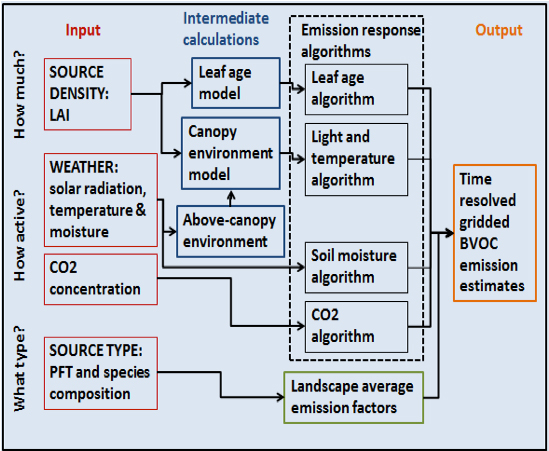
\includegraphics[width=\textwidth]{Figures/MEGANmodel_img.jpg}
      \caption{MEGAN schematic, copied from \textcite{Megan_Website}}
      \label{Models:GC:Isop:MEGAN:fig_megan_schematic}
    \end{figure}
    
    GEOS-Chem V10.01 uses MEGAN V2.1 with biogenic emissions from \textcite{Guenther2012}.
    It computes some emissions using predefined EF maps from MEGAN source code, and others using PFT maps and associated EFs.
    MEGAN ``is a modelling framework for estimating fluxes of biogenic compounds between terrestrial ecosystems and the atmosphere to account for the major known processes controlling biogenic emissions.'' \parencite{Guenther2012}.
    It allows parameterisation of various BVOC emissions, with descriptions given in \textcite{Guenther2012}.
    
    MEGAN was developed as a replacement for two earlier canopy-environment emission models (BIES and GEIA), and initially included a simple canopy radiative transfer model, which parameterised sun-lit and shaded conditions through a canopy.
    Early models didn't account for abiotic stresses, such as drought, prior rainfall and development processes. These stresses influenced species-specific emissions by more than an order of magnitude \parencite{Niinemets1999}.
    Isoprene emissions were based on temperature, leaf area, and light, but have since been updated to include leaf age activity \parencite{Guenther2000}, and a leaf energy balance model \parencite{Guenther2006} in MEGANv2.0.
    This update included a parameter for soil moisture, to account for drought conditions, however this parameter is currently (as of version 2.1) not applied to isoprene \parencite{Sindelarova2014}.
    Soil moisture effects on isoprene emission are very important, and can affect estimates.
    
    Instructions to run version 2.1 are available at \url{http://lar.wsu.edu/megan/docs/MEGAN2.1_User_GuideWSU.pdf}, and a version using the Community Land Model (CLM) is available at \url{http://www.cesm.ucar.edu}.
    It uses meteorological fields from the Weather Research and Forecasting (WRF) modelling system.
    Version 2.1 (updated from 2.0 \parencite{Guenther2006}) includes 147 species, in 19 BVOC classes, which can be lumped together to provide appropriate output for mechanisms in various chemical models.
  
  \subsection{Rescaling NOx}
  
    NO$_X$ concentrations affect HCHO yield, isoprene lifetimes, and other things due to affects on the atmospheres oxidative capacity.
    This means that if the model is poorly simulating NO$_X$, isoprene to HCHO yield and transport (see \ref{BioIsop:Methods:Smearing}) may be poorly estimated.
    In order to determine if rescaling the NO emissions over Australia is necessary in GEOS-Chem, I looked at modelled NO$_2$ amounts compared to satellite data for most of 2005.
    
    % Geos chem vs tropno2 from omno2d
    Simulated GEOS-Chem tropospheric NO$_2$ columns averaged from 1300-1400~LT are compared against OMNO2d data (Sec. \ref{Model:Datasets:OMNO2d}). 
    Figure \ref{Model:Analysis:NOx:fig_GC_vs_OMNO2d_summer_2005} shows the direct comparison between these datasets averaged over the month of January, 2005.
    It's clear that the OMNO2d product can pick out Sydney and Melbourne as NO$_2$ hotspots, which are underestimated by GEOS-Chem due to averaging over the 2x2.5\degr horizontal resolution.
    Over much of the country GEOS-Chem overestimates NO$_2$ by 10-60\%, except in NA and northern Queensland where up to 50\% underestimation occurs.
    The correlation between the bias (GEOS-Chem - OMNO2d) with anthropogenic and soil emissions is shown in the bottom rows.
    The comparison for January and February of 2005 in Figure \ref{Model:Analysis:NOx:fig_GC_vs_OMNO2d_summer_2005}, and winter (JJA) of 2005 in Figure \ref{Model:Analysis:NOx:fig_GC_vs_OMNO2d_winter_2005}.
    The poor correlations for anthropogenic NO suggest that blanket alterations over Australia would not lead to improved NO$_2$ fit. 
    
    \begin{figure}
      % Figure from GC_tests.py GC_vs_OMNO2d, then modified in paint
      % Summer correlation
      \includegraphics[width=\textwidth]{Figures/OMI_link/GC/GC_vs_OMNO2_AUS_20050101-20050228.png}
      \caption{%
        Row 1 shows the tropospheric columns in molec cm$^{-2}$, GEOS-Chem, OMNO2d, and OMNO2d averaged onto the lower resolution of GEOS-Chem from left to right.
        Row 2 shows the correlations of GEOS-Chem (X axes) between daily anthropogenic emissions, and mid-day OMNO2d columns.
        Row 3 shows the differences with OMNO2d columns averaged into the lower resolution of GEOS-Chem.
      }
      \label{Model:Analysis:NOx:fig_GC_vs_OMNO2d_summer_2005}
    \end{figure}
    
    \begin{figure}
      % Figure from GC_tests.py GC_vs_OMNO2d, then modified in paint
      % Winter correlation
      \includegraphics[width=\textwidth]{Figures/OMI_link/GC/GC_vs_OMNO2_AUS_20050601-20050831.png}
      \caption{%
        As figure \ref{Model:Analysis:NOx:fig_GC_vs_OMNO2d_summer_2005}, for winter 2005.
      }
      \label{Model:Analysis:NOx:fig_GC_vs_OMNO2d_winter_2005}
    \end{figure}
    
    This comparison is expanded, including a comparison against modelled emissions, and repeated for autumn (MAM), winter (JJA), and spring (SON) in figures \ref{Model:Analysis:NOx:fig_GC_vs_OMI_anthro_Sum} to \ref{Model:Analysis:NOx:fig_GC_vs_OMI_soil_Spr}.
    These show an analysis of GEOS-Chem NO emissions and their correlations with the bias between GEOS-Chem NO$_2$ mid-day columns and the OMNO2d product, averaged over each season in 2005.
    The scatter plots have one datapoint for each land square over Australia.
    
    The correlation between model and satellite NO$_2$ columns is OK throughout the year over Australia, with some overestimation in the north during non-summer months.
    There is also slight underestimation over Sydney and Melbourne throughout the year.
    Figures \ref{Model:Analysis:NOx:fig_GC_vs_OMI_anthro_Sum} to \ref{Model:Analysis:NOx:fig_GC_vs_OMI_soil_Spr} show that the visible biases are not driven by modelled emissions of NO.
    While the correlation between column NO$_2$ and emitted NO is clear, emissions do not appear to bias the model in either direction away from the satellite data.
    
    % Figures from GC_tests.py GCe_vs_OMNO2d
    \mypic{Figures/OMI_link/GC/GCanthro_vs_OMNO2_AUS_20050101-20050228.png}
    {
      Top row (left to right): GEOS-Chem NO$_2$ mid-day tropospheric columns, OMNO2d NO$_2$ columns, modelled anthropogenic NO emissions. 
      Second row: absolute and relative difference between GEOS-Chem and OMI NO$_2$ data, and the correlation.
      Third row: correlation between GEOS-Chem tropospheric column NO$_2$ and emitted NO, then between the model-satellite bias and the emissions.
      All correlation plots are coloured by emission rates.
    }
    {\label{Model:Analysis:NOx:fig_GC_vs_OMI_anthro_Sum}}
    
    \mypic{Figures/OMI_link/GC/GCanthro_vs_OMNO2_AUS_20050301-20050531.png}
    {As figure \ref{Model:Analysis:NOx:fig_GC_vs_OMI_anthro_Sum}, for Autumn 2005.}
    {\label{Model:Analysis:NOx:fig_GC_vs_OMI_anthro_Aut}}
    
    \mypic{Figures/OMI_link/GC/GCanthro_vs_OMNO2_AUS_20050601-20050831.png}
    {As figure \ref{Model:Analysis:NOx:fig_GC_vs_OMI_anthro_Sum}, for Winter 2005.}
    {\label{Model:Analysis:NOx:fig_GC_vs_OMI_anthro_Win}}
    
    \mypic{Figures/OMI_link/GC/GCanthro_vs_OMNO2_AUS_20050901-20051130.png}
    {As figure \ref{Model:Analysis:NOx:fig_GC_vs_OMI_anthro_Sum}, for Spring 2005.}
    {\label{Model:Analysis:NOx:fig_GC_vs_OMI_anthro_Spr}}
    
    % Soil pictures
    \mypic{Figures/OMI_link/GC/GCsoil_vs_OMNO2_AUS_20050101-20050228.png}
    {As figure \ref{Model:Analysis:NOx:fig_GC_vs_OMI_anthro_Sum}, except anthropogenic NO emissions are replaced by soil NO emissions.}
    {\label{Model:Analysis:NOx:fig_GC_vs_OMI_soil_Sum}}
    
    \mypic{Figures/OMI_link/GC/GCsoil_vs_OMNO2_AUS_20050301-20050531.png}
    {As figure \ref{Model:Analysis:NOx:fig_GC_vs_OMI_anthro_Sum}, for Autumn 2005, with soil NO emissions replacing anthropogenic NO emissions.}
    {\label{Model:Analysis:NOx:fig_GC_vs_OMI_soil_Aut}}
    
    \mypic{Figures/OMI_link/GC/GCanthro_vs_OMNO2_AUS_20050601-20050831.png}
    {As figure \ref{Model:Analysis:NOx:fig_GC_vs_OMI_anthro_Sum}, for Winter 2005, with soil NO emissions replacing anthropogenic NO emissions.}
    {\label{Model:Analysis:NOx:fig_GC_vs_OMI_soil_Win}}
    
    \mypic{Figures/OMI_link/GC/GCanthro_vs_OMNO2_AUS_20050901-20051130.png}
    {As figure \ref{Model:Analysis:NOx:fig_GC_vs_OMI_anthro_Sum}, for Spring 2005, with soil NO emissions replacing anthropogenic NO emissions.}
    {\label{Model:Analysis:NOx:fig_GC_vs_OMI_soil_Spr}}
    
    The conclusion drawn is that modelled anthropogenic and soil NO emissions do not show sufficient evidence of biasing GEOS-Chem NO$_2$ columns away from satellite measurements over Australia.
    For this reason modelled NO emissions are not scaled in model runs in this thesis.
  
  
  
  \subsection{GEOS-Chem outputs}
    \label{Model:GC:outputs}
    There are various outputs available when running GEOS-Chem, which require understanding in order to compare with observations.
    % Default time step and resolution of GC outputs
    GEOS-Chem in this thesis is run with a 15 minute time step for both chemistry and transport, at 2x2.5\degr horizontal resolution over 47 vertical levels.
    Generally output is the average of these time steps either over an entire month, or else per day.
    
    In my work when estimating model yields of isoprene to HCHO, I use daily averaged HCHO columns and compare them to colocated isoprene emissions from MEGAN.
    Optionally one can save high temporally resolved data for a single (or list of) column(s).
    I've used this diagnostic to compare modelled ozone with ozonesonde profiles at three sonde release sites discussed in Chapter \ref{Ozone}.
    
    
    \begin{description}
      \item[Satellite overpass]%
        is output from averaging over a window of local time for each gridbox. 
        This output allows comparison with satellite measurements, which overpass at the same local time every day.
        This diagnostic allows easier analysis of model data against a satellite as one can match the output with the satellite's overpass time.
        Output averaged between 1300-1400 LT is saved to allow comparisons with Aura satellite measurements, as Aura overpasses at $\sim$1330 LT each day.
        This has been performed by others \parencite[eg.][]{Jin2017}.
      \item[HEMCO diagnostics]%
        % Local time offsets
        In order to get hourly MEGAN modelled isoprene emissions, HEMCO (the module of GEOS-Chem dealing with emissions inventories) diagnostic output was created.
        When working with globally gridded data, handling local time offsets becomes more important.
        The hourly output emissions of isoprene is saved using GMT, which needs to be offset based on longitude in order to retrieve local time.
        I do this by setting up a latitude by longitude array which matches the horizontal resolution of the data, filling each gridbox with it's local time offset.
        This offset is determined as one hour per 15 degrees (since 360 degrees is 24 hours), and then used to retrieve global data at any specific local time.
        The retrieval of a daily local time global array is done by index matching the GMT+LT (modulo 24) with the desired hour on this grid over the 24 GMT hours.
        are the emissions TODO: averaged or instantaneous? in each gridbox, which I've stored for each 3 hours.
      \item[Tracer averages]%
        are daily or monthly averaged gridbox concentrations.
      
    \end{description}
     
  \subsection{GEOS-Chem simulations}
    \label{Model:GC:runs}
    
    GEOS-Chem is run four independent times in this thesis, with different outputs from each simulation used to determine specific information. 
    Output averaged over 1300 - 1400 local time is saved for comparison with, and recalculation of, satellite overpass records.
    These averages are used to calculate both the GEOS-Chem based AMF, and the modelled background HCHO over the remote pacific which is used in the reference sector correction for OMI column retrievals (see section \ref{Model:omiRecalc:RSC}).
    They are also used to determine isoprene to HCHO yield, after removing days with high biomass burning emissions.
    
    TODO: Go through work process and clarify these items
    Run descriptions and their outputs are listed here, with outputs described in more detail in section :
    \begin{enumerate}
      \item UCX 
      \begin{enumerate}
        \item Satellite output (1300-1400LT)
        \item Create shape factors for AMF recalculation in OMI
        \item This run was initially used to determine if the stratospheric chemistry had much influence over tropospheric isoprene or HCHO concentrations.
      \end{enumerate}
      
      \item Tropchem (standard)
      \begin{enumerate}
        \item satellite output, daily tracer averages
        \item Recreate the AMFs for OMI when running code from Dr. Paul Palmer, modified by Dr. Luke Surl.
        \item Combined with an identical run where isoprene emissions are halved in order to determine smearing.
        \item TODO: Compare total yearly isoprene emissions before and after new estimate.
      \end{enumerate}
      
      \item Tropchem(isoprene emissions halved)
      \begin{enumerate}
        \item In GEOS-Chem the isoprene emissions can be globally multiplied by a constant factor.
        \item An estimate of modelled HCHO sensitivity to isoprene emissions and transport (smearing) can be determined.
        \item Smearing is determined by running the model with the biogenic isoprene emissions halved while other parameters remain unchanged.
      \end{enumerate}
      
      \item Tropchem(biogenic emissions only, all other inventories turned off)
      \begin{enumerate}
        \item Satellite output, hourly biogenic emissions from MEGAN
        \item The output from this simulation is used to determine the biogenic yield from isoprene to HCHO over Australia, described in section \ref{BioIsop:Methods}.
        \item TODO: compared to run with updated emissions
      \end{enumerate}
      
    \end{enumerate}
    NB: for non-UCX runs, satellite output was modified to include tropopause height
    
    
    % TODO: layout reasons why isoprene differs between runs
    %    In GeosCore/fast_jx_mod.F:
    %      strat aerosols are scaled somehow at line 2922, looks like it affects SSA.
    %      line 4138: comment says ozone calculated online.
    %	  TOMS/SBUV O3 are read by toms_mod.f, passed to FAST-J routine ``set_prof.f''. in UCX the stratospheric O3 is calculated online
    %    In GeosCore/calcrate.F:
    %      line 1489 comment says rates are limited to prevent solver failure
    %	if lifetime of A is below PSCMINLIFE, limit reaction rate to yield the specified lifetimedepletion
    %      Line 1724
    %        ! SPECIAL TREATMENT FOR O3+hv -> OH+OH (trop-only simulation)
    %        !                    or O3+hv -> O+O2  (UCX simulation)
    %      line 1752:
    %      #if defined( UCX )
    %        IF ( NKO3PPHOT(NCS) > 0 ) THEN
    %          PHOTVAL_2 = NKO3PPHOT(NCS) - NRATES(NCS)
    %          NKN_2     = NKNPHOTRT(PHOTVAL_2,NCS)
    %        ENDIF
    %      #endif
    %      line 1771:
    %        comment: change rate of O(1D) + N2 to 3.1e-11 at 298K (from 2.6e-11)...
    %        if not defined UCX:
    %	  RO1Dp1H2O, RO1Dp1H2, RO1D, (and maybe 2 RRates) are changed.
    
    \subsubsection{Run comparisons}
    
    There are many options available when running GEOS-Chem depending on the desired chemistry, resolution, meteorology, and boundary conditions.
    Here we compare the model output with and without enabling the Universal tropospheric-stratospheric Chemistry eXtension (UCX).
    %From version 11 of GEOS-Chem, the UCX mechanism is enabled by default.
    Both runs use 2$^{\circ}$ latitude by 2.5$^{\circ}$ longitude, however the UCX mechanism is run with 72 vertical levels from the surface to the top of the atmosphere (TOA$\sim$0.1~hPa), while the standard (tropchem) run uses 47 levels.
    The extra vertical levels are added in the stratosphere, providing finer vertical resolution from around 70~hPa to the top of the atmosphere.
    For both runs the inpup parameters such as MEGAN emissions and GEOS-5 meteorological fields are identical.
    
    GEOS-Chem output of HCHO does not differ much between runs with or without the Unified Chemistry eXchange (UCX).
    Figure \ref{Model:GC:running:fig_UCXvsTrop_HCHO} shows an example of surface HCHO amounts with and without UCX turned on.
    The differences do not exceed 3\% over Australia for the averaged month of January, 2005.
    
    \begin{figure}%[!htbp] % TODO: remove 'rerun' plot, use normal and delete rerun thingy so it's not confusing later.
      % These figures created in GC_test.py -> TODO:
      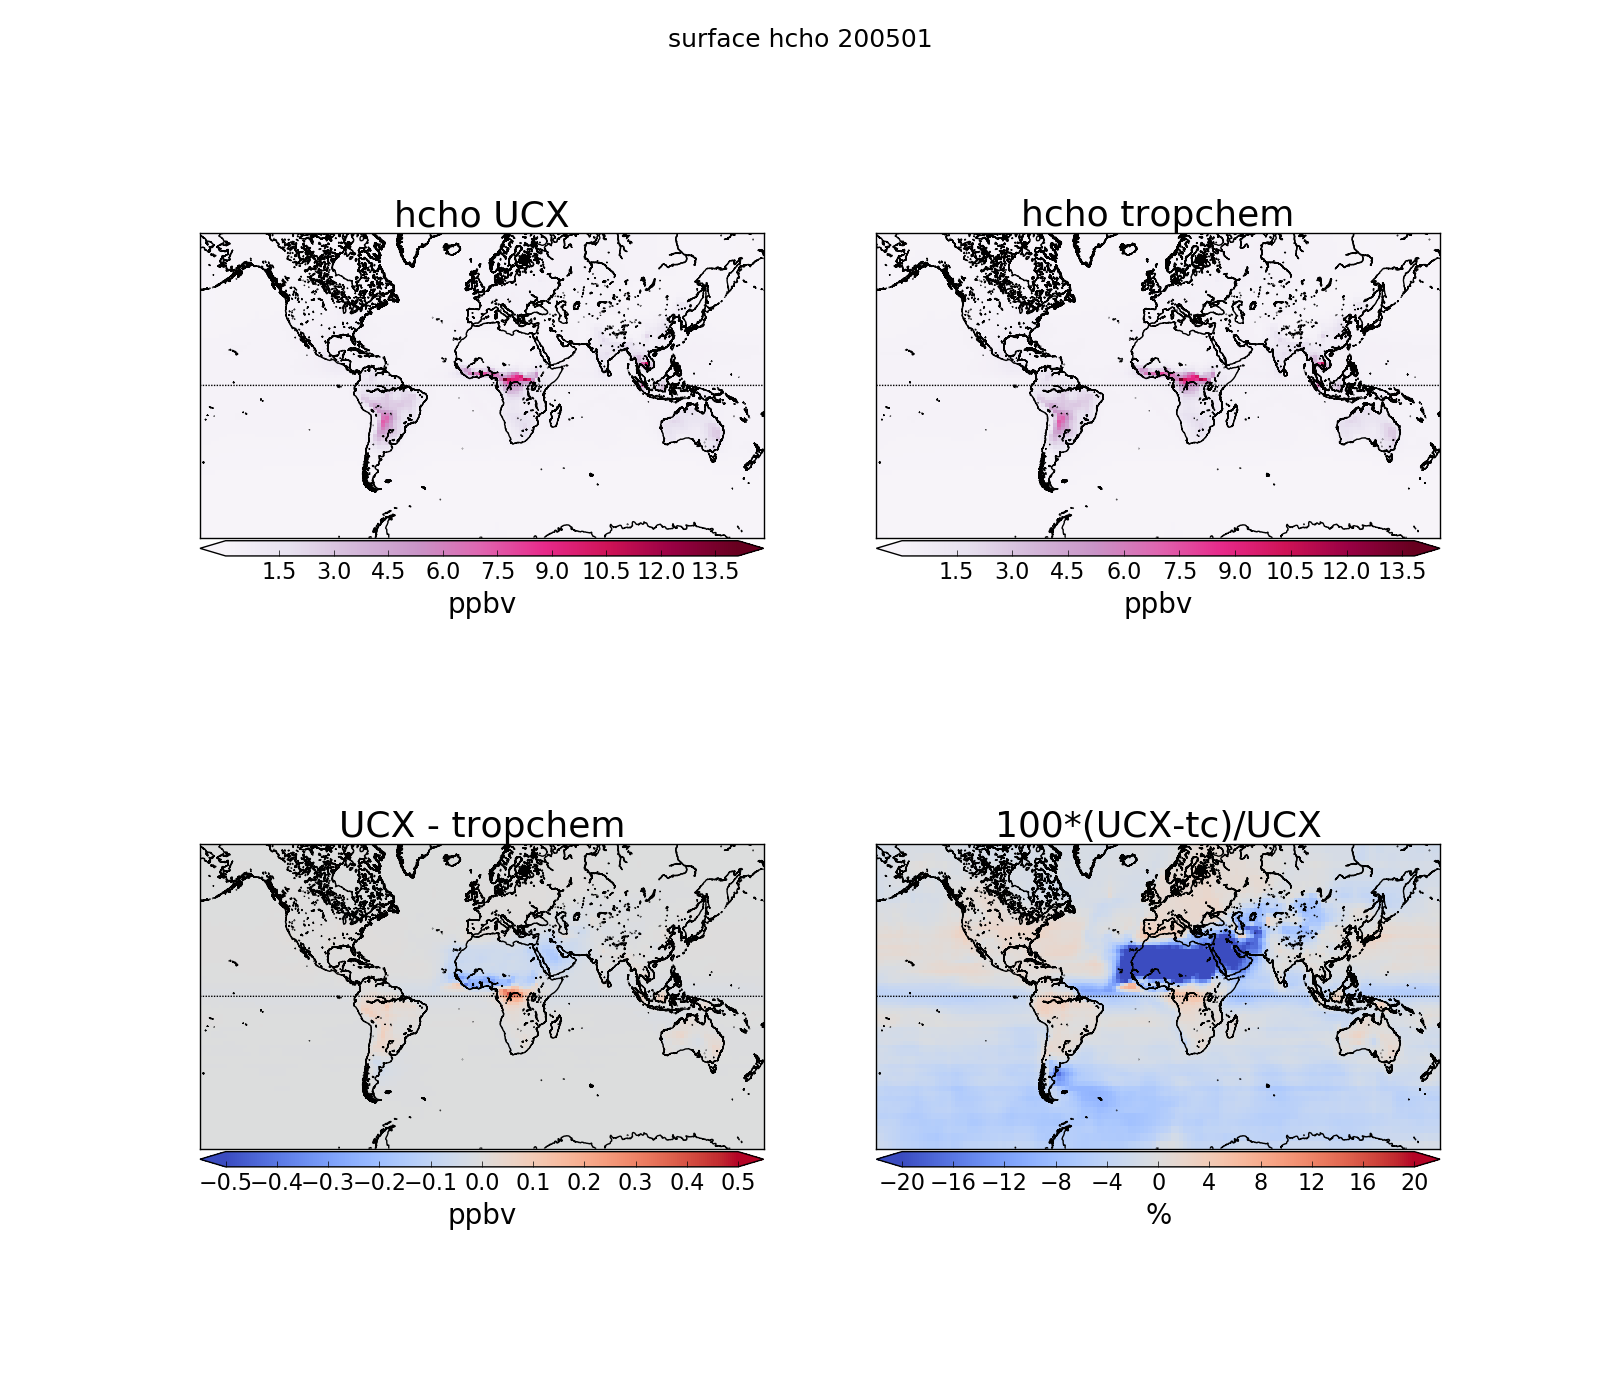
\includegraphics[width=\textwidth]{Figures/OMI_link/GC/UCX_vs_trp_glob_200501_hcho_rerun.png}
      \caption{ %
        Surface HCHO simulated by GEOS-Chem with UCX (top left), and without UCX (top right), along with their absolute and relative differences(bottom left, right respectively).
        Amounts simulated by GEOS-Chem for the 1st of January, 2005.
      }
      \label{Model:GC:running:fig_UCXvsTrop_HCHO}
    \end{figure}
    
    Figure \ref{Model:GC:running:fig_UCXvsTrop_Isop} shows the differences in surface isoprene amounts over Australia.
    Here we start to see a higher relative difference in concentrations, although this is generally over the areas with less absolute concentrations. 
    Very little isoprene is seen away from the continent (4-5 orders of magnitude less), due to the short lifetime of isoprene, and lack of emissions over the oceans.
    Generally isoprene is 0-30\% higher over Australia when the UCX mechanism is turned on.
    This enhancement can be seen throughout the entire tropospheric column as shown by Figure TODO fix ref \ref{ch_HCHO:fig:isoptropUCXcomparison}. %TODO: fix ref
    \begin{figure}
      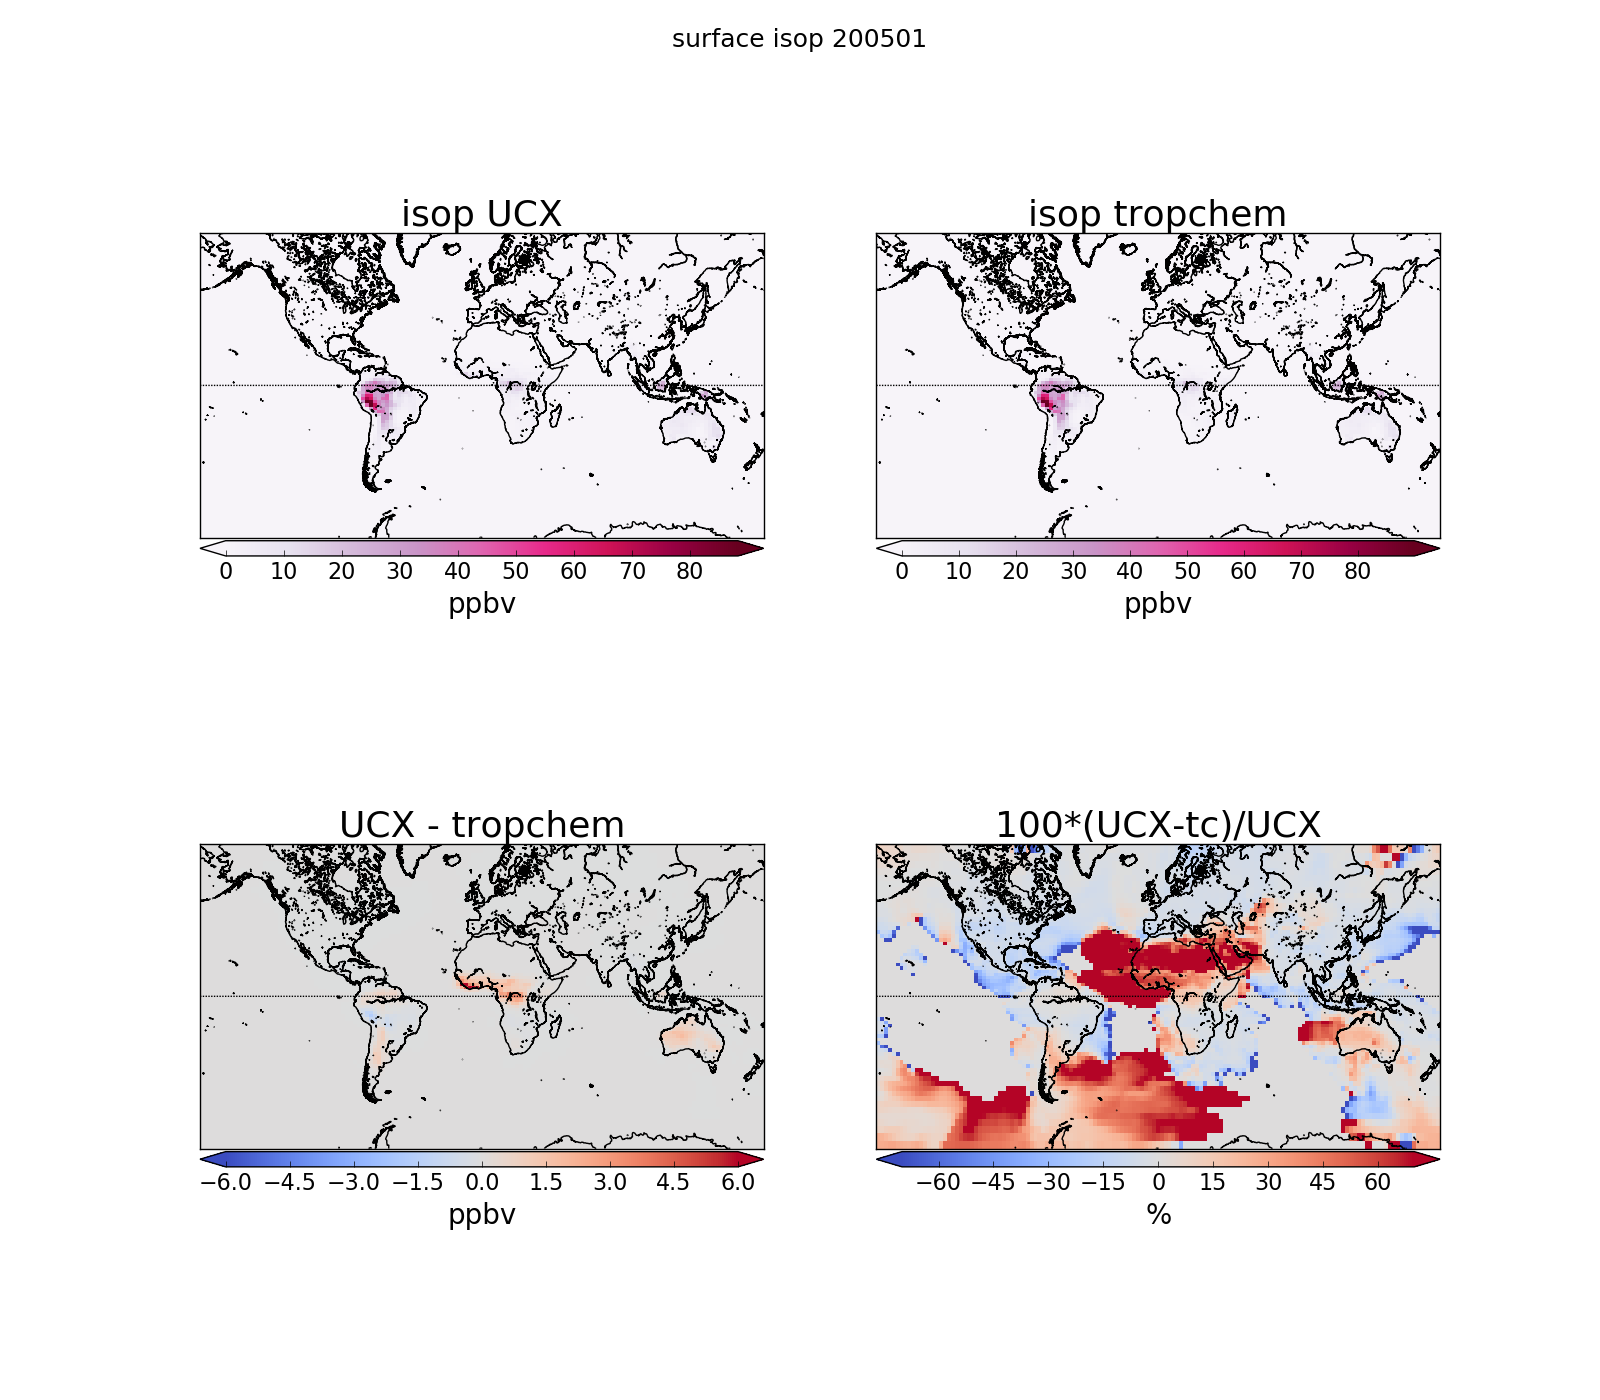
\includegraphics[width=\textwidth]{Figures/OMI_link/GC/UCX_vs_trp_glob_200501_isop_rerun.png}
      \caption{ %
        As figure \ref{Model:GC:running:fig_UCXvsTrop_HCHO}, except looking at isoprene. 
      }      
      \label{Model:GC:running:fig_UCXvsTrop_Isop}
    \end{figure}
    
    
    Figure TODO: shows the columns for isoprene and HCHO simulated by our two mechanisms over Australia in January of 2005.
    The differences are minimal compared to other uncertainties in both AMF calculation and emissions estimation.
    
    
    TODO: The difference in isoprene between UCX and tropchem is likely caused by differences in the modelled radiation reaching the troposphere due to differences in simulated ozone in the stratosphere.
    With higher stratospheric ozone levels, less radiation would reach the troposphere, changing the photochemistry.
    Figure \ref{Model:GC:running:fig_UCXvsTrop_O3} shows the total column ozone between UCX and non-UCX runs, we can see that UCX has TODO: less or more ozone over Australia/USA in January.
    
    \begin{figure}
      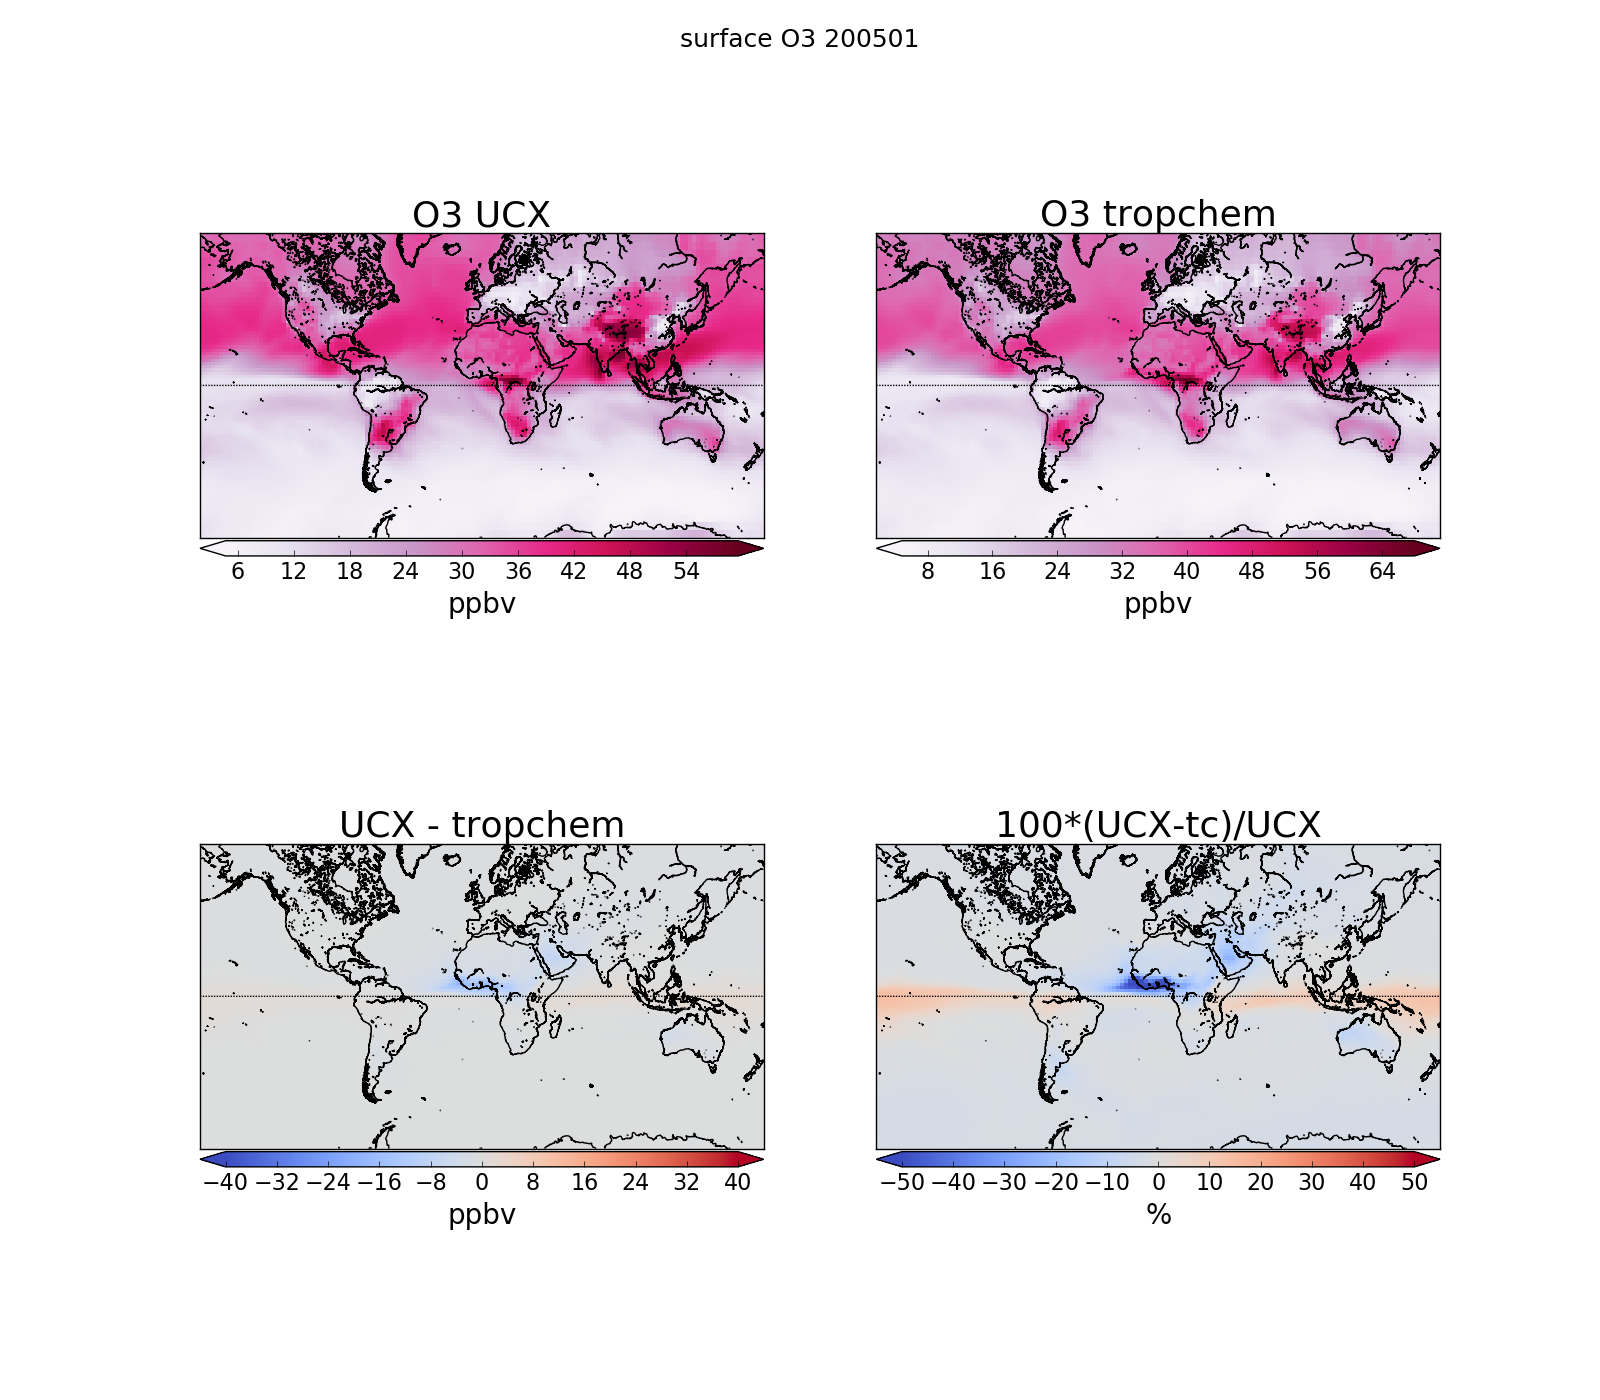
\includegraphics[width=\textwidth]{Figures/OMI_link/GC/UCX_vs_trp_glob_200501_O3_rerun.png}
      \caption{%
        As figure \ref{Model:GC:running:fig_UCXvsTrop_HCHO}, except looking at ozone. 
      }
      \label{Model:GC:running:fig_UCXvsTrop_O3}
    \end{figure}
    
    

      
  \section{Calculating an AMF}
    \label{Model:Meas:AMF}
    
    The AMF is the ratio of the slant column ($\Omega_s$) to the vertical column ($\Omega_v$)
    \begin{equation} \label{Model:Meas:AMF:eqn_AMFFrac}
      AMF=\frac{\Omega_s}{\Omega_v} = \frac{\tau_s}{\tau_v}
    \end{equation}
    with $\tau$ being the optical depth or thickness of the absorber through the slant (\textit{s}) or vertical (\textit{v}) path of light
    
    
    The OMI instrument records spectra of light which enters the viewing lens on board the satellite.
    The spectra provide backscattered intensity ($I_B$) at various wavelengths (see section \ref{Model:Datasets:Aura}), with the light source ($I_{B_0}$) being the sun. 
    Using the log of beers law (equation \ref{Model:Meas:DOAS:eqn_beerslaw}) we get 
    $$ \tau_s = \ln{I_{B_0}} - \ln{I_B} $$
    which can be subbed into equation \ref{Model:Meas:AMF:eqn_AMFFrac} to give an expression for the AMF which includes scattering:
    \begin{equation} \label{Model:Meas:AMF:eqn_amfscattering}
      AMF = \frac{\ln{I_{B_0}}-\ln{I_B}}{\tau_v}
    \end{equation}
    %{Model:Meas:DOAS:eqn_backscatterextinction}
    %$\tau_s$ is the optical thickness of the absorber along the measured path between source and instrument.
    
    We use $\nabla I = I_B - I_{B_0}$ to represent the change in intensity due to the absorber. 
    For optically thin absorption, $\nabla I / I_B << 1$, and we can use:
    \begin{equation} \label{Model:Meas:AMF:eqn_AMFthin}
      AMF = \frac{\ln{ \left( 1 - \frac{\nabla I}{I_B} \right)} }{\tau_v} \approx \frac{ - \frac{\nabla I}{I_B} }{\tau_v}
    \end{equation}
    This is due to the logarithmic property $\ln \left(1-x \right) \approx -x$ for $x<<1$.
    $\nabla I$ can also be expressed as the integral of the absorption slices over optical depth increments: 
    \begin{eqnarray*}
    \nabla I &= \int_0^{\tau_v}{\frac{\partial I_B}{\partial \tau} \mathrm{d}\tau}
    \frac{\nabla I}{I_B} & = \int_0^{\tau_v}{\frac{\partial \ln{I_B}}{\partial \tau} \mathrm{d}\tau}
    \end{eqnarray*}
    which can be placed into equation \ref{Model:Meas:AMF:eqn_AMFthin} leading to
    \begin{equation*}
    AMF \approx \frac{-1}{\tau_v} \int_0^{\tau_v}{\frac{\partial \ln{I_B}}{\partial \tau} \mathrm{d}\tau}
    \end{equation*}
    We can then convert $\text{d}\tau$ to our path using equation \ref{Model:Meas:DOAS:eqn_tau} leading to
    \begin{equation} \label{Model:Meas:AMF:eqn_AMFcross}
    AMF = \frac{-1}{\tau_v} \int_0^\infty {\frac{\partial \ln{I_B}}{\partial \tau} \alpha(z)\eta(z)\mathrm{d}z}
    \end{equation}
    where $\alpha(z)$ and $\eta(z)$ represent absorption cross section in m$^2$ molecule$^{-1}$, and number density in molecules m$^{-3}$ respectively. 
    This uses the attenuation cross section relationship to optical depth (see section \ref{Model:Meas:DOAS}).
    
    To represent an average cross section weighted by the absorbing species' vertical distribution, the effective cross section ($\alpha_e$) is used.
    This is to account for temperature and pressure dependence of $\alpha(z)$, and is defined as:
    \begin{align*}
      \alpha_e &= \frac{1}{\Omega_v} \int_0^\infty \alpha(z) \eta(z) \mathrm{d}z \\
       &= \frac{\tau_v}{\Omega_v}
    \end{align*}
    Then replacing the $\tau_v$ in equation \ref{Model:Meas:AMF:eqn_AMFcross} we obtain:
    \begin{equation} \label{Model:Meas:AMF:eqn_AMFpreomega}
      AMF=-\int_0^\infty{ \frac{\partial \ln{I_B}}{\partial \tau} \frac{\alpha(z)}{\alpha_e} \frac{\eta(z)}{\Omega_v} \mathrm{d}z }
    \end{equation}
    Often the integrand of this AMF formula (equation \ref{Model:Meas:AMF:eqn_AMFpreomega}) is broken apart into two defining terms: the scattering weights $\omega(z)$ and the shape factor $S(z)$.
    \begin{description}
      \item[$\omega$] The scattering weights describing the sensitivity of the backscattered spectrum to the abundance of an absorber at altitude z:
      \begin{equation} \label{Model:Meas:AMF:eqn_omega}
      \omega(z) = -\frac{1}{AMF_G} \frac{\alpha(z)}{\alpha_e} \frac{\partial \ln{I_B}}{\partial \tau}
      \end{equation}
      It's worth noting that in the OMI satellite product, the provided $\omega(z)$ term does not include the $\frac{1}{AMF_G}$ term and a the calculations which follow therefor do not include this term when utilising the provided $\omega$.
      This is not noted in any of the papers which recalculate the AMF from the OMI product, due to them recalculating the $\omega$ term themselves with a radiative transfer model such as LIDORT.
      \item[$S$] the shape factor describes the profile of an absorber ($\eta(z)$) normalised by its total vertical column amount ($\Omega_v$):
      \begin{equation} \label{Model:Meas:AMF:eqn_shapefactor}
        S(z) = \frac{\eta(z)}{\Omega_v}
      \end{equation}
    \end{description}
    
    Plugging equations \ref{Model:Meas:AMF:eqn_omega} and \ref{Model:Meas:AMF:eqn_shapefactor} into equation \ref{Model:Meas:AMF:eqn_AMFpreomega} gives us:
    \begin{equation} \label{Model:Meas:AMF:eqn_AMF_amfgintwSdz}
      AMF = AMF_G\int_0^\infty{ \omega(z) S(z) \mathrm{d}z}
    \end{equation}
    Since we are using the $\omega$ provided by OMI, the AMF$_G$ term is removed from this calculation as it is not part equation \ref{Model:Meas:AMF:eqn_omega} leading to 
    \begin{equation} \label{Model:Meas:AMF:eqn_AMF_intwSdz}
      AMF = \int_0^\infty{ \omega(z) S(z) \mathrm{d}z}
    \end{equation}
    
    Additionally the AMF can be determined using the sigma ($\sigma$) coordinate system.
    A conversion to the $\sigma$ vertical coordinate is performed using $P = \sigma (P_S - P_T) + P_T$, where $P_T$ is pressure at the top of the atmosphere and $P_S$ is surface pressure.
    This can be useful when running global atmospheric models as the ground altitude is always at $\sigma=1$ and we need not worry about topography. 
    $S_\sigma$ is a dimensionless normalised shape factor on the $\sigma$ coordinate system.
    In the sigma coordinate system we calculated the shape factor as defined in \textcite{Palmer2001}:
    \begin{equation} \label{Model:Meas:AMF:eqn_ShapeFactorSigma}
    S_\sigma(\sigma) = \frac{\Omega_a}{\Omega_v}C_{HCHO}(\sigma)
    \end{equation}
    where $\Omega_a$ is the vertical column of air from the surface to the top of the atmosphere and C$_{HCHO}(\sigma)$ is the mixing ratio of HCHO.
    The hydrostatic relation $P = - \rho_a g z$, with $\rho_a$, g, being density of air, gravity, respectively lets us integrate over the sigma coordinates:
    \begin{align*}
    \rho_a g z & = \sigma \left( P_S - P_T \right) + P_T \\
    \mathrm{d}\sigma  & = - \frac{ \rho_a g }{ P_S - P_T } \mathrm{d}z
    \end{align*}
    Substitution into \ref{Model:Meas:AMF:eqn_AMF_intwSdz} gives AMF using the sigma coordinates:
    \begin{equation} \label{Model:Meas:AMF:eqn_AMFintwSdsigma}
    AMF = \int_0^1 w(\sigma) S_\sigma(\sigma) \mathrm{d}\sigma
    \end{equation}

\section{Recalculation of OMI HCHO}
  \label{Model:omiRecalc}
  
  % what is AMF, Omega_V and Omega_S
  The AMF is needed to transform the slant column (SC) viewed by the satellite into a vertical column ($\Omega$):
  \begin{equation}
    \label{Model:omiRecalc:eqn_AMFratio}
    AMF = \frac{SC}{\Omega} %= \frac{\tau_s}{\tau_v}
  \end{equation}
  A slant or vertical column is expressed in molecules cm$^{-2}$.
  % Reiteration of why we recalculate AMFs
  OMI HCHO vertical columns are calculated using modelled a priori HCHO profiles (see section \ref{Model:Datasets:OMHCHO}).
  When comparing satellite measurements against models it is important to recognise the impact of this a priori on the total column values.
  This is due to how the sensitivity of OMI (to HCHO and other trace gases) varies vertically throughout the atmosphere.
  When comparing OMI vertical columns ($\Oo$) to GEOS-Chem ($\Og$), the satellite AMF needs to be recalculated using GEOS-Chem modelled vertical gas profiles as the a prioris.
  Without performing this step a bias between modelled and measured total column values may be due to the a priori rather than chemistry or measurements \parencite{Palmer2001, Lamsal2014}.
  
  % Very brief outline
  Here, two new AMFs are calculated, both using GEOS-Chem HCHO profiles as the new a priori. 
  The first AMF (AMF$_{GC}$) uses the original satellite scattering weights while recalculating the shape factor, whereas the second AMF (AMF$_{PP}$) also recalculates scattering weights.
  AMF$_{PP}$ is created using code initially written by Professor P. Palmer (see sections \ref{Model:omiRecalc:ShapeFactor} and \ref{Model:omiRecalc:ppcode} for more details).
  A reference sector correction is determined using the method described in \textcite{Abad2016}, (see section \ref{Model:omiRecalc:RSC}).
  This correction is unique for each of the 60 \textit{measurement tracks} used by OMI.
  Finally the correction is applied to each pixel to create the corrected vertical column. 
  The end product is three sets of corrected vertical columns (VCC): the original ($\Ooc$), one using GEOS-Chem shape factors ($\Ogc$), and one from Palmer's code ($\Opc$).
  
  \subsection{Outline}
    \label{Model:omiRecalc:outline}
    
    % Summary of actual actions taken:
    Here is an outline in computational order of what takes place when recalculating the $\Omega$ from OMI.
    \begin{enumerate}
      \item GEOS-Chem satellite overpass output (see section \ref{Model:GC:outputs}) is used to create new shape factors (S$_z$ and S$_\sigma$).
      \begin{enumerate}
        \item Pressure edges and geometric midpoints are determined, along with altitudes (\textit{z}), and box heights (H).
        \item Number density and mixing ratio of HCHO ($n_{HCHO}$, $C_{HCHO}$ respectively) are taken or created from model outputs HCHO(ppb) and air density (molec/cm3)
        \item Total column HCHO from GEOS-Chem ($\Og$) is calculated $\Og = \Sigma_z \left(n_{HCHO}(z) \times H(z) \right)$, along with total column air ($\Omega_{A}$, calculated similarly)
        \item The shape factor S$_z(z)$ is calculated on each altitude $S_z(z) = n_{HCHO} / \Omega_{HCHO}$.
        \item Pressures (\textit{p})are used to create sigma coordinates $\sigma(z) = (p(z) - p_{TOA}) / (p(0)-p_{TOA})$
        \item S$_\sigma(z)$ is calculated on each altitude: $S_\sigma(z) = C_{HCHO}(z) \times \Omega_A / \Omega_{HCHO}$
      \end{enumerate}
      \item Satellite pixels (SC, scattering weights ($\omega(z)$), pressure levels, latitude and longitude) are read from the OMHCHO dataset.
      \item For each pixel, a new AMF (AMF$_{GC}$)is created using the GEOS-Chem shape factors and satellite scattering weights.
      \begin{enumerate}
        \item scattering weights ($\omega$) are interpolated onto the same vertical dimensions (\textit{z} and $\sigma$) as the shape factors.
        \item Integration (approximated using rectangular method) is performed along the vertical dimension to calculate the new AMF on both coordinate systems.
        \begin{align}
          AMF_z &= \Sigma_z \left(\omega(z) \times S_z(z) \times H(z)\right) \\
          AMF_s &= \Sigma_{\sigma} \left(\omega(\sigma) \times S_{\sigma}(\sigma) \times d\sigma \right)
        \end{align}
      \end{enumerate}
      \item These two AMFs represent the same thing using different coordinates. Either one can be used as the AMF$_{GC}$.
      \item The AMF$_{PP}$ (created separately) and AMF$_{GC}$ are used to determine the new vertical columns ($\Op$, $\Og$ respectively): $\Omega = SC/AMF$.
      \item A reference sector correction (RSC) is defined each day using these AMFs along with modelled HCHO over the remote pacific.
      \begin{enumerate}
        \item GEOS-Chem satellite overpass output ($\Omega_{GEOS-Chem}$ from 140{\degr}W to 160{\degr}W) are averaged monthly and longitudinally to provide a modelled reference sector $\Omega_0[lat]$.
        \item The modelled reference slant columns (\textit{MRSC}) are calculated using $MRSC = \Omega_0 \times AMF$ for each AMF.
        \item For each satellite pixel between 140{\degr}W and 160{\degr}W, the correction is calculated as the measured \textit{SC} minus the \textit{MRSC} at the nearest latitude.
        \begin{equation*}
          corr[lat,track] = SC[lat,track] - MRSC[lat]
        \end{equation*}
        \item These corrections are binned by satellite detector (track: 1-60), and latitude (0.36\degr; 500 latitudes from 90{\degr}S to 90{\degr}N).
        \item The median entry of each bin is determined and this forms the RSC[lat,track] (eg. figure \ref{Model:omiRecalc:RSC:fig_track_correction_interpolations})
      \end{enumerate}
      \item VCC are determined using $VCC = (SC - RSC[lat,track] )/AMF$ for each measured SC and using each AMF, with the RSC linearly interpolated to the latitude of the satellite pixel.
      \item The VCC (along with most of the pixel and GEOS-Chem data) are binned onto a 0.25\degr by 0.3125\degr grid along with how many pixels have been binned, and the average pixel uncertainty in product OMHCHORP.
    \end{enumerate}
  
    Figure \ref{Model:omiRecalc:fig_flow_omhchorp} shows an overview of how these profiles are used in this thesis.
    Output from GEOS-Chem is combined with OMHCHO swath data to produce a gridded HCHO file which contains HCHO vertical columns recalculated with GEOS-Chem a prioris.
    PP code is run on a subset of the globe covering Australia and the pacific ocean, producing AMF$_{PP}$.
    The output keeps the original AMF as well as those recalculated using GEOS-Chem (AMF$_{OMI}$, AMF$_{GC}$, and AMF$_{PP}$).
    Additionally, MOD14A1, OMAERUVd and OMNO2d data are used to create masks which are also stored in the OMHCHORP dataset.
    The creation of fire, smoke, and anthropogenic influence masks is described in section \ref{Model:Filter}.
    
    \mypic{Figures/Flow_Making_omhchorp.png}{Flow diagram showing how OMHCHO level two swath data is read, processed, and gridded in this thesis}{\label{Model:omiRecalc:fig_flow_omhchorp}}
      
    
    
  \subsection{Creating new shape factors}
    % Reminder of AMF -> leading to what is the shapefactor
    In order to visualise and analyse OMI HCHO columns, slant columns are transformed into vertical columns using the AMF.
    The shape factor (\textit{S}) is one of the key components in creation of the AMF (see section \ref{Model:Meas:AMF}, equation \ref{Model:Meas:AMF:eqn_AMF_intwSdz}).
    The shape factor is calculated using GEOS-Chem satellite output (see section \ref{Model:GC:outputs}) which provide simulated HCHO concentration profiles ($\eta(z)$) and total columns ($\Omega$) at 2x2.5\degr horizontal resolution.
    Using equation \ref{Model:Meas:AMF:eqn_shapefactor} to determine the shape factor is straightforwards $S(z) = \frac{\eta(z)}{\Omega}$.
    The associated OMI per-pixel scattering weights are not changed in this calculation (unlike in section \ref{Model:omiRecalc:ppcode}).
    
    Model output is in molecules per billion molecules of air (ppb), and is converted before being used in the shape factor calculation.
    The following equation converts model profile output from ppb into number densities:
    \begin{equation} \label{Model:omiRecalc:eqn_ppb_to_n}
      \eta_{HCHO} = ppb_{HCHO} \times \eta_a \times 10^{-9}
    \end{equation}
    where $\eta_{HCHO}$ is the number density of a HCHO, $\eta_a$ is the number density of air (from model output), and ppb$_{HCHO}$ is the molecules of that species per billion molecules of air.
    The modelled total vertical column $\Omega_{HCHO}$ is determined by:
    \begin{equation*}
      \Omega_{HCHO} = \Sigma_z \left( \eta_{HCHO} \times H(z) \right)
    \end{equation*}
    where H(z) is the box height for level z.
    In effect this equation sums over the molecules per cm$^2$ in each altitude level.
    
    As a sanity check I also recalculate $S_\sigma$ (through equation \ref{Model:Meas:AMF:eqn_ShapeFactorSigma})and confirm that these shape factors are equivalent by comparing the resulting AMFs created by equation \ref{Model:Meas:AMF:eqn_AMFintwSdsigma} and equation \ref{Model:Meas:AMF:eqn_AMF_intwSdz} for each pixel.
    %TODO: Shape factor plot sigma vs z
    For example see figure TODO: sigma vs z shape factor plot.
    TODO add plot and describe here.
    
    
  \subsection{Reading satellite data}
    
    % Downloading the data
    First satellite slant columns of formaldehyde for the years January 1st, 2005 - April 1st, 2013 are downloaded (see section \ref{Model:Datasets:OMHCHO}).
    The data set used is from the Ozone Monitoring Instrument (OMI) on board the Aura satellite, as it has data for the entire time line and sufficiently covers the southern hemisphere.
    % Filters applied when reading
    When reading OMHCHO level 2 swath files, several factors are taken into account in order to filter uncertain and erroneous pixels.
    The process is outlined in figure  \ref{Model:omiRecalc:fig_flow_omhchorp} for a single day.
    First all \textit{good} pixels (those with QA flag equal to 0) are read into a long list (roughly 1 million per day).
    These are then filtered by solar zenith angle (SZA) and latitude, similarly to other works \parencite[eg.]{Marais2012, Barkley2013, Bauwens2016, Zhu2016}.
    This filtering removes highly uncertain pixels, along with those for which instrument problems such as the OMI row anomaly (see section \ref{Model:Datasets:OMHCHO}) may have affected.
    
    % Actual filtering done
    Satellite measurements polewards of 60\degr north or south are removed as well as measurements with SZA greater than 60\degr.
    Pixels with cloud fraction greater than 40\% are removed after being used in determining the reference sector correction (see section \ref{Model:omiRecalc:RSC}), as is done in \textcite{Abad2015, DeSmedt2015}.
    Further filtering is performed to remove the measurements which are most likely to be unrealistic: those with column density outside the range $-0.5 \times 10^{16}$ to $10^{17} $\moleccm, as is performed by\textcite{Zhu2016}.
    This filter is required due to currently unexplained large negative values which occur in the OMI HCHO product increasingly over time.
    Figure \ref{Model:omiRecalc:fig_OMI_negative_hist} shows how unfiltered HCHO columns are affected by a small set of highly negative values which heavily affect the mean column amount over any region.
    The histograms here show the negative (left) and positive (right) total column HCHO measurements from a subset of swaths over Australia, on the 18th of March 2013.
    The highly negative values can be seen around the $-10^{19}$~molecules cm$^{-2}$ region.
    
    \mypicw{1\textwidth}{Figures/AusOMHCHO_Hist_20130318.png}
    {
      Column density histograms for a subset of OMI swaths over Australia on the 18th of March 2013.
      Negative entries are shown in the left panel, positive in the right, note the different scale between negative and positive panels.}
    {\label{Model:omiRecalc:fig_OMI_negative_hist}}
    
    % reading pixels into a long list
    Each pixel and it's relevant data are saved in a long list, around $1.1$ million pixels per day.
    Additional information is added to each pixel, such as the new AMF calculated through replacing the a priori vertical profile with the newer GEOS-Chem simulated profile.
    The shape factors and scattering weights for each pixel lie along a z-axis which is vertically resolved to 47 layers.
    
    
  
  % How we get the a priori 
  \subsection{Creating the new AMF}
    \label{Model:omiRecalc:ShapeFactor}
    
    From equation \ref{Model:Meas:AMF:eqn_AMF_intwSdz} we have:
    $$ AMF = \int_0^\infty \omega(z) S(z) \mathrm{d}z $$
    then using the $\omega(z)$ from satellite output, along with our calculated $S_z$ interpolated linearly onto the same vertical grid as $\omega(z)$, the AMF can be determined through integration.
    The integration is done in Python using a simple rectangular method, which multiplies the integrand midpoints by the change in height, and then takes the sum.
    This assumes that the provided scattering weights and shape factors are linear between the 47 resolved values.
    
      
    
  \subsection{Recalculating the AMF using PP code}
    \label{Model:omiRecalc:ppcode}
    % pp code for AMF recalculation referred to as pp code
    
    Some of the pixels (those covering Australia and most of the zonal band) have their AMFs recalculated using Fortran code written by Paul Palmer, Randal Martin, and updated by Luke Surl.
    I will refer to this as the PP code, and subscript the VCs and AMFs with PP when referring to those calculated through this method.
    This code is computationally expensive, and is only run on pixels within within the region (50-10\degr~S, 160\degr~W-160\degr~E).
    The Fortran code uses a combination of GEOS-Chem a priori profile information and satellite measurement data to calculate the AMF after running the LIDORT radiative transfer calculations to determine scattering.
    The instrument sensitivity or scattering weights and shape factors for each pixel are calculated within the PP code, which outputs AMF$_{PP}$.
    
    
    Code for recalculating AMFs using satellite swaths and modelled aerosol optical depths and gas profiles can be found at \url{http://fizz.phys.dal.ca/~atmos/martin/?page_id=129}. 
    The original method for HCHO is layed out in \textcite{Palmer2001}, with modifications for clouds and use of the LIDORT RTM \parencite{Spurr2002} as described by \textcite{Martin2003}.
    This code does not work as is when using OMI satellite data, and requires modifications performed by Luke Surl at Edinburgh University.
    Additionally the tropopause heights averaged within satellite overpass times output by GEOS-Chem is required, which is achieved by modifying the ND51 diagnostic.
    
    Mie scattering and clouds can complicate the calculation of $\omega$(z), however tables of values for this function at various parameter inputs can be used with modeled vertical shape factors for local AMF calculations.
    This has been done in the PP code and the AMF look-up-table (LUT) can be found in the source code at TODO: add git repo with this code.
    In order to run, output is required from GEOS-Chem: the HCHO concentration profile averaged between 1300 and 1400 LT, including optical depths at several wavelengths (TODO: list), and dust concentrations.
    A subset of the OMI pixel information is also required, which is coalesced from OMHCHO daily swath files into csv files (one per day), which can be read by the PP code as modified by Dr. Luke Surl, in conjunction with the GEOS-Chem outputs for each day.
    The PP code then produces a csv of recalculated AMFs which get read by my python code and associated with the corresponding pixel (outlined in \ref{Model:omiRecalc:fig_flow_omhchorp}).
    
  \subsection{Vertical columns from AMF}
    
    All that remains for recalculating the total vertical column using our new a priori shape factor is to apply the new AMF to the slant columns and grid them onto our chosen resolution.
    Each satellite pixel at this stage has an associated SC along with three AMFs: the original (AMF$_O$), one with recalculated shape factors (AMF$_G$), and one completely recalculated using PP code (AMF$_{PP}$).
    These are used to create vertical columns ($\Omega$) through equation \ref{Model:Meas:AMF:eqn_AMFFrac}: $\Omega = SC/AMF$.
    
    Figure TODO shows a comparison between the three $\Omega$ over Australia for 2005. 
    The first row shows the yearly average column amounts, as well as coloured rectangles describing regions which are averaged over time in row 3.
    Row two from left to right shows the relative differences between $\Op$ and $\Og$, $\Oo$ and $\Og$, and $\Oo$ and $\Op$.
    TODO: Add this plot here.
    
  \subsection{Reference sector correction}
    \label{Model:omiRecalc:RSC}
    % where we apply the RSC
    Each satellite slant column measurement is corrected by some amount, based on the divergence from a modeled reference sector.
    HCHO products from OMI and SCIAMACHY both use a median daily remote pacific ocean radiance reference spectrum, over 15$^{\circ}$S-15$^{\circ}$N, 140$^{\circ}$-160$^{\circ}$W where it is assumed that the only significant source of HCHO is methane oxidation \parencite{DeSmedt2008,Barkley2013,Kurosu2014}.
    
    % What RSC does
    The RSC method corrects for several problems, however it introduces some a priori model influence.
    One of the problems removed through this correction method is instrument degradation, which can introduce bias over time.
    Another is the possible influence of varying dead/hot pixel masks across 2-D detector arrays such as OMI \parencite{DeSmedt2015}.
    This method also corrects for the errors introduced through correlations between BrO and HCHO absorption cross sections, which are especially significant at high latitudes \parencite{Abad2015}.
    
    % How Vertical columns use reference sector corrections
    Vertical columns in OMI use this oceanic background instead of a solar irradiance spectrum
    In order to recalculate the vertical columns using modelled data, a RSC needs to be applied.
    The correction uses the difference between the slant column ($\Omega_S$) and the reference slant column ($\Omega_{S_0}$) divided by the AMF, plus the modelled reference sector column ($\Omega_{V_B}$):
    \begin{equation*}
      \Omega_{VC} = \frac{ \left( \Omega_S - \Omega_{S_0} \right) }{ AMF } + \Omega_{V_B}
    \end{equation*}
    This method is used in various papers, including \textcite{DeSmedt2008, DeSmedt2012, DeSmedt2015, Barkley2013, Bauwens2016}.
    Recently this correction was expanded (for OMI data) to include latitudinal and instrument track influence by \textcite{Abad2015}.
    
    % How my RSC is defined
    The reference sector correction (RSC) for OMI satellite pixels in this thesis is calculated following \textcite{Abad2016}.
    A correction is created based on the difference between the background HCHO measurements (OMI slant columns) and the GEOS-Chem modelled HCHO columns ($\Omega_0$) within the reference sector (140{\degr}W to 160{\degr}W).
    To get the modelled slant columns, each of the AMFs (calculated in prior sections) is applied to the modelled vertical columns using equation \ref{Model:omiRecalc:eqn_AMFratio}.
    % Then RSC Longitudinally averaged, binned into 500 lats
    The longitudinal average is taken within the a priori reference sector, as corrections are assumed to be longitudinally invariant.
    The modeled reference sector is averaged over the month and interpolated latitudinally to 500 equidistant bins.
    Figure \ref{Model:omiRecalc:RSC:fig_RSCeg} shows the simulated reference sector VCs as an example, calculated for January 1st 2005.
    In this figure the vertical resolution is increased from 2$^{\circ}$ to 0.36\degr, through linear interpolation, in order to form 500 vertical bins which are used in correcting the satellite data.
    Each day, good satellite measurements taken over the reference sector are used to determine a correction array.
    The model does not produce slant columns associated with each measurement, however one is created by multiplying the vertical column with the associated slant column's AMF.
    
    % This picture was made where?!
    \mypicw{0.7\textwidth}
    {Figures/HCHO/Summary_RSC_Effect8d_20050101.png}
    {%
      Example of remote pacific RSC using 8-day average measurements and one month modelled data.
      $\Omega_{VC}$ shows the uncorrected vertical columns, while $\Omega_{VCC}$ shows the corrected vertical columns.
      OMI corrections shows the correction applied globally based on latitude and OMI track number(sensor).
      $\Omega_{GC}$ shows the GEOS-Chem modelled HCHO VC over the RSC, with $\Omega_{VCC}$ showing the corrected VC over the same area.
    }
    {\label{Model:omiRecalc:RSC:fig_RSCeg}}
    
    % Swath RSC corrections are done 'per track'
    For OMI swaths, each row of measured data contains 60 `Across track'(track) measurements.
    The track index (i) relates a the measurement to one of the 60 columns of data.
    Corrections for each measurement are calculated by taking the difference between the measured slant column and the a priori slant column as follows:
    \begin{equation} \label{Model:omiRecalc:eqn_RSC}
      Correction(i,j) = SC_{HCHO}(i,j) - VC_{GEOS-Chem}(lat(j)) \times {AMF}(i,j)
    \end{equation}
    where j represents a latitude index and $VC_{GEOS-Chem}(lat)$ represents the a priori reference sector vertical column HCHO at the latitude corresponding to j.
    Note that the correction is in molecules cm$^{-2}$.
    % Correction applied over each of the 60 tracks
    The RSC is independently calculated for each of the 60 tracks, at each latitude in the 500 0.36\degr bins.
    This provides a different RSC 
    
    % Interpolated daily RSC to cover missing latitudes
    Due to incomplete latitudinal coverage, the correction for each track is interpolated linearly between measurements, with corrections outside of the highest measured latitudes being equal to the corrections at the highest measured latitudes.
    Figure \ref{Model:omiRecalc:RSC:fig_track_correction_interpolations} shows an example of the 60 track corrections for January 1st 2005, the points are satellite measurements longitudinally averaged over the remote pacific, coloured by track number.
    \mypicw{0.7\textwidth}{Figures/OMI_link/RSC_track_corrections20050101.png}
      {Example of track correction interpolations for January 1st 2005, points represent the difference between satellite slant column measurements and modelled slant columns over the remote pacific.}
      {\label{Model:omiRecalc:RSC:fig_track_correction_interpolations}}
    
    % Visualisation of RSC refering to plot and 8-day averaged corrections
    Another way to look at this correction is given in the OMI corrections panel of figure \ref{Model:omiRecalc:RSC:fig_RSCeg}, which has the sensors along the x axis, and latitude on the y axis, and shows how for this example 8-day period, the corrections are distributed with more negative values towards the left or right sensors, especially in the tropics.
    
    % One correction per pixel, based on latitude and omi track
    One correction is associated with every good satellite measurement which is used to create a reference sector corrected measurement (Vertical Column Corrected or VCC) through the following equation:
    \begin{equation}
    VCC(i,j) = \frac{SC_{HCHO}(i,j) - Correction(i,lat(j))}{AMF(i,j)}
    \end{equation}
    Finally, for each day, the good satellite measurements are averaged into our own latitude longitude resolution bins along with the associated corrected SC, VC, VCC, AMF, and bin entry count.
    The bin entry count is used to create weighted averages from the daily binned data, which accounts for sparse entries due to filtering.
  
  \subsection{Binning the results daily}
    
    Finally the pixels are binned into a gridded dataset I've called OMHCHORP, as shown in figure \ref{Model:omiRecalc:fig_flow_omhchorp}.
    The resolution is chosen to match the native resolution of GEOS-Chem (0.25x0.3125\degr) and the GEOS met data fields.
    %TODO: list of things stored in the daily omhchorp outputs
    Data averaged into this dataset are as follows:
    \begin{enumerate}
      \item satellite SC %($\Omega_{S}$)
      \item satellite AMF %(AMF$_{OMI}$)
      \item satellite VC %($\Omega_{V,OMI}$
      \item satellite RSC VC %($\Omega_{VC,OMI}$)
      \item GEOS-Chem recalculated AMF %(AMF$_{GC}$)
      \item GEOS-Chem recalculated VC %($\Omega_{V,GC}$)
      \item GEOS-Chem recalculated RSC VC %
      \item GEOS-Chem AMF recalculated using Paul Palmer code (AMF$_{PP}$)
      \item GEOS-Chem RSC VC based on AMF$_{PP}$
      \item Smoke AAOD from OMAERUVd (mapped into bins from 1x1\degr resolution)
      \item satellite pixel counts (summed into bins)
      \item fire counts (summed into bins)
    \end{enumerate}
    
    TODO: time per regridding and reprocessing:
    This whole process requires some processing time as well as RAM and computer storage space, and has been performed on the National Computing Infrastructure (NCI) supercomputer cluster.
    In order to reprocess one year of swath files, X GB of daily data was downloaded and then transformed into Y GB of daily gridded data.
    This takes around 90 minutes per day, and is very parallelisable as each day is completely independent once the model has run in each required configuration.
    Initially paralellism was built into the python code, however simply running sending seperate 'jobs' to NCI's process queue was simpler and more scalable.
    As much as possible, processing is done using the HDF-5 or NetCDF-4 formats, with some GEOS-Chem output being read from bitpunch.
    The scripts to regrid and reprocess the swath data set are available from github at TODO.
  
  \subsection{Difference between new and old OMI HCHO columns}
  
    
    New corrected vertical columns (VCC) of HCHO are created at global 0.25 by 0.3125\degr horizontal resolution.
    These calculations are compared over Australia in figure(s) TODO: Map comparison, regression, and time series.
    The effect of not recalculating the $\omega_z$ is can be seen in figure \ref{Model:omiRecalc:fig_VCC_pp_fires} which looks at the altered satellite vertical columns using each method.
    Figure \ref{Model:omiRecalc:fig_VCC_pp_fires} shows vertical columns of HCHO for: column 1) the original satellite swaths, column 2) recalculated without changing the provided scattering weights, and column 3) fully recalculated vertical columns. 
    Each grid square (at 0.25 by 0.3125\degr lat lon resolution) has been created by binning the recalculated satellite pixels within the month.
    The average pixels per land square is inset as text, changing due to how the fire filter is applied.
    Each row has a stricter fire filter applied from top to bottom, with no fire filter on the first row up to filtering pixels from squares with fires up to 8 days prior.
    This figure looks at March 2005 with biomass burning filtered differently in each row.
    Active fires over the last 0, 1, 2, 4, and 8 days are filtered as the row number increases.
    
    %TODO: figure analysing amf vs amf_gc vs amf_pp
    Figure TODO shows an analysis of the differences between running the recalculation with and without updating the $\omega_z$.
    
    \mypic{Figures/OMI_link/VCC_fires_20050301-20050331.png}{% 
      Column 1: Reference sector corrected HCHO vertical columns $\Omega$ from OMHCHOv003.
      Column 2: $\Omega$ with recalculated a priori shape factors using GEOS-Chem v10.01.
      Column 3: $\Omega$ with recalculated a priori shape factors and scattering weights using GEOS-Chem v10.01 and LIDORT.
      Row 1-5: increasing number of prior days which have active fires are included when masking fire influence.
      }{\label{Model:omiRecalc:fig_VCC_pp_fires}}
    
    TODO: Ask luke if this is true:
    The AMF calculated using Dr. Palmer's code uses a more strict series of filters, leading to fewer satellite based HCHO columns and reduced coverage over Australia.
    Stricter filtering must be balanced against both coverage and the sensitivity of the AMF determination to recalculating $\omega_z$.
  
    Figure TODO: shows global and Australian HCHO averaged total column maps for January 2005, along with the reduced major axis (RMA) regression correlation and percentage difference.
    This comparison shows how reprocessing with an updated model can have a systematic influence on the total column.

\section{Filtering Data}
  \label{Model:Filter}
  
  % Why filter data
  In order to examine only biogenic processes, pyrogenic and anthropogenic influences need to be removed from modelled and measured data.
  Biomass burning can be a large local or transported (via smoke plumes) source of HCHO, CHOCHO, glyoxal, and other compounds which influence levels of both HCHO and isoprene.
  Anthropogenic emissions from power generation, transport, and agriculture can influence these levels as well.
  Where possible these influences need to be removed so that calculations of purely biogenic emissions are not biased. 
  In GEOS-Chem we can simply turn off pyrogenic and anthropogenic emissions, however in satellite datasets we need to mask potentially affected pixels.
  
  % How other people have filtered fires
  Influence from biomass burning can be removed through measurements of acetonitrile and CO (eg: \parencite{Wolfe2016, Miller2017}, or else removal of scenes coincident with satellite detected fire counts and aerosol absorption optical depth as done in \textcite{Marais2014}.
  \textcite{Marais2012} remove pixels colocated with non zero fire counts in any of the prior eight days, within grid squares with 1 x 1\degr resolution.
  \textcite{Barkley2013} use fires from the preceding and concurrent day, within local or adjacent grid squares, with grid resolution of 0.25 x 0.3125\degr.
  \textcite{Wolfe2016} disregard HCHO measurements when acetonitrile > 210~pptv and CO > 300~ppbv, while acetonitrile > 200~pptv is used to determine fire influence in \textcite{Miller2017}.
  TODO: look at yearly correlation, compare to exponential curve and look for fire outliers
  As seen in TODO: citation, HCHO concentrations scale exponentially with temperature.
  This allows another method for detecting the influence of non-biogenic HCHO emission/creation by looking for outliers above the curve at low temperature.
  \textcite{Zhu2013_poster} has a similar analysis over south-eastern USA showing an exponential correlation of ${HCHO} = \exp(0.15*{T}-9.07)$.
  
  I use satellite data to account for anthropogenic and pyrogenic influences on the OMHCHO satellite HCHO columns.
  MODIS fire counts are used in conjunction with smoke AAOD enhancements (from OMI) to remove data points which may be affected by fires or fire smoke plumes.
  OMI NO$_2$ measurements are used to mask potential anthropogenic influence.  
  These masks negatively affect uncertainty,  as fewer measurements are available to be averaged.
  This section describes the creation and effects of filters used on satellite data.
  
  A quick summary of how much data is filtered over Australian land squares is provided in table TODO, and an quick check of how many pixels are filtered in January 2006 can be seen in Figure \ref{Model:Filter:fig_pixel_loss_Jan06}.
  The majority of fire filtering can be seen in Queensland, potentially due to gas flaring and mining hotspots which could be assessed as fire pixels by the MODIS active fires product. 
  Other fire hot-spots occur over port Kembla, Perth, and Mount (remote WA) TODO find map showing that this is probably true.
  The anthropogenic filter completely removes grid squares over Sydney and Melbourne, and high removal rates over Brisbane. 
  Other major cities in Australia either do not emit enough NO$_2$ or are too spread out and do not breach the threshold to be filtered as anthropogenic.
  
  \mypic{Figures/OMI_link/Filters/PixelsFiltered_20060101-20060131.png}{Top row shows grid squares filtered out by pyrogenic(left) and anthropogenic(right) influence masks during January 2006. Along the bottom is the time series of total pixels over Australian land squares with and without filtering the data.}{\label{Model:Filter:fig_pixel_loss_Jan06}}
  
  
  \subsection{Fire and smoke}
    \label{Model:Filter:fire}
    
    
    The method used in this thesis follows that of \textcite{Marais2012}, and \textcite{Barkley2013}, with active fires filtered using fire counts, and smoke filtered out using smoke aerosol absorption optical depth (AAOD).
    We use the MODIS fire counts, detected from space using the combined product from Terra and Aqua (Terra at 10:30, 22:30 LT; Aqua at 13:30, 01:30 LT).
    Smoke plumes are filtered using smoke AAOD from product OMAERUVd, with the threshold determined through analysis of Australian AAOD distributions.
    
    % My method for fire filtering:
    OMHCHO total column HCHO $\Omega$ is processed into a 0.25x0.3125\degr horizontal daily grid.
    Pyrogenic filters are created as follows. 
    They are created or interpolated to the same the same horizontal resolution as $\Omega$ to simplify application. 
    The following steps are performed in order to create the pyrogenic influence mask:
    \begin{enumerate}
      \item MOD14A1 daily gridded Aqua/Terra combined fire counts (1x1~km$^2$) are read, and binned into 0.25x0.3125\degr bins (matching the resolution of binned $\Omega$).
      \item A rolling mask is formed which removes $\Omega$ if one or more fires are detected in a grid square, or in the adjacent grid square, up to 2 days previously.
      This includes the 'current' day, making 3 days of fires in total being filtered out on each day.
      \item AAOD at 500~nm is mapped from OMAERUVd (1x1\degr resolution) onto the 0.25x0.3125\degr resolution.
      \item An AAOD threshold of 0.03 is determined through visual analysis of AAOD distributions over several days, including days with and without influence from active fires, dust, and transported smoke plumes (see figure \ref{Model:Filter:fire:fig_typicalAAOD}).
      \item Grid squares with AAOD over this threshhold are considered potentially affected by transported fire smoke.
    \end{enumerate}
  
    % Smoke AAOD filtering:
    Determining the AAOD due to smoke can be difficult since both smoke and dust absorb UV radiation \parencite{Ahn2008,Marais2012}.
    AAOD is less sensitive to cloud contamination than AOD, and I use AAOD from the daily gridded level 3 satellite product OMAERUVd \parencite{Ahn2008} described in section \ref{Model:Datasets:OMAERUVd} to provide a filter for smoke plumes.
    Although removing gridsquares with dust reduces how much data is available to analyse, it's considered a minor problem as dust in Australia is highly episodic and should not affect more than a few days per year, especially over regions with high tree coverage \parencite{Shao2007}.
    
    % Threshold for AAOD determination
    Filtering fire smoke using AAOD is done by removing OMHCHO gridsquares where the AAOD is above a 0.03, after the AAOD is mapped from 1x1\degr to the same 0.25x0.3125\degr resolution as our OMHCHO gridded product.
    The threshhold is determined through analysing AAOD over Australia in 4 scenarios: normal conditions, active local fires, during influence from transported fire smoke, and large scale dust storms.
    Figure \ref{Model:Filter:fire:fig_typicalAAOD} shows AAOD (columns 1 and 2), with AAOD distribution in column 3, along with satellite imagery on the same day in column 4 (from \url{https://worldview.earthdata.nasa.gov/}).
    The scenarios listed are shown from row 1 to 4, and AAOD $=$ 0.03 is demarked by a horizontal line in the density plots in column 3.
    
    \mypic{Figures/OMI_link/typical_AAODs.png}
      {AAOD from OMAERUVd (columns 1, 2, 3) over Australia for four different scenarios (rows 1-4). Scenes from the same day are taken from the EOS Worldview website \url{https://worldview.earthdata.nasa.gov/}.}
      {\label{Model:Filter:fire:fig_typicalAAOD}}
    
    %
    Figure \ref{Model:Filter:fire:fig_portion_filtered_2005} shows what portion of pixels are filtered out by the pyrogenic filter. 
    The top panel shows the spatial distribution of fire masks, with most pixels removed along the northern and eastern coastlines.
    Central Australia is largely unmasked, which could be due to a lack of sufficient vegetation to create a large enough fire to be seen by satellite.
    %Even though transported smoke plumes from South America and southern Africa would influence the measurements in the area.
    One clear hotspot is located over port Kembla (south of Sydney), most likely due to the flame which burns over the blast furnace stack throughout the year.
    Another hotspot can be seen in Western Australia over Kalgoorlie, where a large open cut gold mine ``super pit'' is always open and blasting daily.
    In Western Queensland over Mount Isa there is again a mining related hotspot.
    A large area in southern Queensland/northern NSW is also heavily filtered, potentially due to gas flaring in the Surat Basin, which has thousands of petrol and gas wells.
    A large portion of the 'lightly' filtered areas appear to correspond to forested areas (see figure \ref{Model:Filter:fire:fig_forest_coverage}).
    The other potential cause of pyrogenic filtering is the proliferation of petrol or gas wells (see figure \ref{Model:Filter:fire:fig_petrol_wells} and figure \ref{Model:Filter:fire:fig_gas_lands}).
    The filtering shown here is for 2005, when 388 gas wells existed in Queensland, however more than 2000 wells (cumulative) were approved by 2013, so this may cause more filtering over the course of this thesis' timeline \parencite{Carlisle2012}.
    To check this the filtering portion for 2012 is also plotted in Figure TODO: plot map of filtered squares for 2012 when it's been run by NCI.
    
    
    \mypic{Figures/OMI_link/Filters/Pyrogenic_20050101-20060101_annotated.png}
    {Top: Portion of 2005 filtered out by fire and smoke masks. Bottom: portion filtered out each day from land squares in Australia.}{\ref{Model:Filter:fire:fig_portion_filtered_2005}}
    
    \mypic{Figures/Wells_AUS.png}{Petrol Well locations over Australia (current-2018) (\url{http://dbforms.ga.gov.au/www/npm.well.search})}{\label{Model:Filter:fire:fig_petrol_wells}}
    
    \mypic{Figures/Gas_AUS.jpg}{Gas fields and pipelines (2018) for Australia (\url{http://www.ga.gov.au/scientific-topics/energy/resources/petroleum-resources/gas})}{\label{Model:Filter:fire:fig_gas_lands}}
    
    \mypic{Figures/Australiasforests_2016.png}{Forest coverage, coloured by predominant tree species.}{\ref{Model:Filter:fire:fig_forest_coverage}}
  
    \subsubsection{Checking that fire masks are influencing pyrogenic HCHO}
      
      Looking at temperature can provide evidence of pyrogenic HCHO.
      HCHO precursors are heavily tied to temperature (TODO:cite), and model output shows how higher temperature leads to an increase in HCHO levels.
      Figures \ref{Model:Analysis:HCHO:fig_hcho_vs_temp_SEA_200501} - \ref{Model:Analysis:HCHO:fig_hcho_vs_temp_SWA_200501} show the relationship between temperature and HCHO, for January 2005, within subsets of Australia.
      A reduced major axis regression is used to determine the correlation between surface temperature (X axis) and HCHO (Y axis)..
      Using the natural log of HCHO we can take the linear regression and then exponentiate each side in the equation $\ln{Y} = m{X}+b$ to get ${Y} = \exp{m{X}+b}$. 
      This gives us the exponential fit as shown, with the correlation coefficient between $\ln{HCHO}$ and temperature.
      The distributions of exponential correlation coefficients and exponential 'm' terms is shown in the embedded plot, with one datapoint available for each grid square where the regression is performed.
      
      
      One cause of high HCHO at lower temperatures is direct or transported emissions and subsequent products from biomass burning.
      We test the fire mask by examining the relationship between modelled temperature and satellite HCHO with and without applying the filters for smoke and active fires.
      Figures TODO-TODO show the exponential fits for one month of datapoints (January 2005) in Northern, Southeastern, and Southwestern Australia respectively.
      Each grid square (2 by 2.5\degr) provides one datapoint per day, with satellite HCHO initially averaged onto the lower resolution of the GEOS-Chem modelled surface (from 0 to $\sim 100$~m) temperature
      The scatter between HCHO and temperature is coloured by fire counts, and we see TODO.
      The TODO lines show the exponential fit before and after filtering fire and smoke.
      TODO plot showing how fire mask affects HCHO - Temperature relationship
      
      
      \begin{figure}
        \includegraphics[width=\textwidth]{Figures/OMI_link/GC/HCHO_vs_temp_SEA_20050101-20050228.png}
        \caption{%
          Top panel: surface temperature averaged over January and February 2005.
          Bottom panel: surface temperature correlated against temperature over, with different colours for each gridbox, and the combined correlation. 
          A reduced major axis regression is used within each gridbox (shown in top panel) using daily overpass time surface temperature and HCHO amounts (ppbv).
          The distribution of slopes and regression correlation coefficients (one datapoint per gridbox) for the exponential regression is shown in the embedded plot.
          }
        \label{Model:Analysis:HCHO:fig_hcho_vs_temp_SEA_200501}
        \end{figure}
          
        \begin{figure}
          \includegraphics[width=\textwidth]{Figures/OMI_link/GC/HCHO_vs_temp_NA_20050101-20050228.png}
          \caption{%
            As figure \ref{Model:Analysis:HCHO:fig_hcho_vs_temp_SEA_200501} but for northern Australia.
            }
          \label{Model:Analysis:HCHO:fig_hcho_vs_temp_NA_200501}
        \end{figure}
          
        \begin{figure}
          \includegraphics[width=\textwidth]{Figures/OMI_link/GC/HCHO_vs_temp_SWA_20050101-20050228.png}
          \caption{%
            As figure \ref{Model:Analysis:HCHO:fig_hcho_vs_temp_SEA_200501} but for south-western Australia.
            }
          \label{Model:Analysis:HCHO:fig_hcho_vs_temp_SWA_200501}
        \end{figure}
  
  \subsection{NOx}
    \label{Model:Filter:NOx}
    
    % Why filter high NO? Anthro influence
    Enhanced NO$_2$ concentrations can indicate anthropogenic influence over Australia.
    In order to filter out these influences on satellite HCHO measurements, a filter is designed using the OMNO2d product which includes tropospheric NO$_2$ columns.
    
    % Nox analysis from OMNO2d
    OMNO2d from 2005 is used to determine a suitable threshhold for anthropogenic influence by looking at NO$_2$ columns near several major cities in the south eastern sector of Australia.
    The mean, standard deviation, and time series over Australia of tropospheric NO$_2$ seen by Aura is shown in figure \ref{Model:Filter:NOx:fig_omno2_timeseries}.
    The average tropospheric NO$_2$ column averaged within all of Australia and then each region shown in this figure is listed in table TODO \ref{Model:Filter:NOx:tab_summary}.
    
    \mypic{Figures/OMI_link/OMNO2_timeseries_2005.png}
    {Mean (top left) and standard deviation (top right) of OMNO2d daily 0.25x0.25\degr tropospheric cloud filtered NO$_2$ columns. Time series for Australia, and each region (by colour) shown in the bottom panel, with mean for that region shown on the right. A grey shaded area depicts the 25th to 75th percentiles of Australia averaged NO$_2$ columns for each day in the time series, with a thicker black line showing the Australia-wide mean value.}
    {\label{Model:Filter:NOx:fig_omno2_timeseries}}
    
    % Filters and Threshhold determination and reasoning
    Anthropogenic influences on the NO$_2$ columns are clearly visible near major cities in Australia.
    A filter is created each year from the OMNO2d product in two steps:
    \begin{enumerate}
      \item Daily gridsquares with NO$_2$ greater than 10$^{15}$\moleccm  are flagged as anthropogenic.
      \item After taking the yearly average over Australia, any gridsquares greater than $1.5 \times 10^{15}$\moleccm are flagged for the whole year.
    \end{enumerate}
    This removes both the gridsquares close enough to cities to be affected by their emissions year round, as well as effects from transported pollution plumes.
    The affects of applying this filter to the OMNO2d product itself can be seen in figure \ref{Model:Filter:NOx:fig_omno2_threshaffect}
    
    \mypic{Figures/OMI_link/OMNO2_threshaffect_2005.png}
    {2005 OMNO2d NO$_2$ column mean before (left) and after (right) applying the threshhold filters as described in the text. Time series for Australia, and each region (by colour) shown in the bottom panel, with mean for that region shown on the right.}
    {\label{Model:Filter:NOx:fig_omno2_threshaffect}}
    
    % Threshhold analysis
    The same regions as in figure \ref{Model:Filter:NOx:fig_omno2_timeseries} are shown again in figure \ref{Model:Filter:NOx:fig_omno2_densities}, with NO$_2$ pixels densities for each region shown, along with the threshold of $1 \times 10^{15}$\moleccm.
    This led to a reduction of TODO gridsquares from the total available measurement space over Australia.
    The removal of gridsquares which went above the yearly averaged limit of 1.5e15\moleccm further reduced the available data by TODO gridsquares.
    
    \mypic{Figures/OMI_link/OMNO2_densities_2005.png}
    {2005 OMNO2d NO$_2$ column means (top left), along with column amount distributions for Australia (top right) and each region shown in the area map (by colour)}
    {\label{Model:Filter:NOx:fig_omno2_densities}}
    
    \begin{table}
      \caption{NO$_2$ averages by region before and after filtering for anthropogenic emissions using 2005 data from the OMNO2d product.}
      \begin{tabular}{ c c c c }
        \hline
        \textbf{Region} & \textbf{NO$_2$} & \textbf{NO$_2$ after filtering} & \textbf{\% Data lost} 
        \\ \hline
        Aus & 1 & 2 & 3 \\
        BG & 1 & 2 & 3 \\
        Syd & 1 & 2 & 3 \\
        Melb & 1 & 2 & 3 \\
        Adel & 1 & 2 & 3 \\
        \hline
      \end{tabular}
      \label{Model:Filter:NOx:tab_summary}
    \end{table}
    
    % Affects of filtering
    % TODO: tabulate or summarise no2 filtering
    
    \subsection{Summary of filters effects on HCHO}
      
     
\section{Data Access}
TODO: ADD MORE HERE
\label{Model:DataAccess}
\begin{description}
  \item[OMNO2d] Daily satellite NO$_2$ product downloaded from \url{https://search.earthdata.nasa.gov/search}, DOI:10.5067/Aura/OMI/DATA3007. 
  See more information in section %TODO:
  
  \item[SPEI] Monthly standardised precipitation evapotranspiration index (metric to determine drought stress) downloaded from \url{http://hdl.handle.net/10261/153475} with DOI:10.20350/digitalCSIC/8508.
  See more information in section %TODO:
  
  \item[OMHCHO] Satellite swaths of HCHO slant columns downloaded from TODO, with DOI TODO
  
\end{description} % Modelling with GEOS-Chem
    %% CHAPTER 3 (probably)
%% Ozone paper

%\begin{document}
%  \title{Stratospheric ozone intrusion events and their impacts on tropospheric ozone in the Southern Hemisphere}
%  
%  % \Author[affil]{given_name}{surname}
%  \Author[1]{Jesse W.}{Greenslade}
%  \Author[2,3]{Simon P.}{Alexander}
%  \Author[4,5]{Robyn}{Schofield}
%  \Author[1,6]{Jenny A.}{Fisher}
%  \Author[2,3]{Andrew K.}{Klekociuk}
%  
%  \affil[1]{Centre for Atmospheric Chemistry, School of Chemistry, University of Wollongong, Australia}
%  \affil[2]{Australian Antarctic Division, Hobart, Australia}
%  \affil[3]{Antarctic Climate and Ecosystems Co-operative Research Centre, Hobart, Australia}
%  \affil[4]{School of Earth Sciences, University of Melbourne, Australia}
%  \affil[5]{ARC Centre of Excellence for Climate System Science, University of New South Wales, Australia}
%  \affil[6]{School of Earth \& Environmental Sciences, University of Wollongong, Australia}
%  
%  \runningtitle{Southern Hemisphere stratospheric ozone intrusions}
%  \runningauthor{Greenslade et al.}
%  \correspondence{Jesse Greenslade (jwg366@uowmail.edu.au)}


\chapter{Stratospheric ozone intrusions} % Main chapter title
\label{ch_StratOzone} %better reference name like ch_HCHO

%----------------------------------------------------------------------------------------
%	SECTION
%----------------------------------------------------------------------------------------

\section{Introduction}
  Tropospheric ozone constitutes only 10\% of the total ozone column but is an important oxidant and greenhouse gas which is toxic to life, harming natural ecosystems and reducing agricultural productivity.
  Over the industrial period, increasing tropospheric ozone has been estimated to exert a radiative forcing (RF) of 365~mWm$^{-2}$  \citep{Stevenson2013}, equivalent to a quarter of the CO$_2$ forcing \citep{IPCC_Chapter2}. 
  While much tropospheric ozone is produced photochemically from anthropogenic and natural precursors, %from NO$_x$ and volatile organic compounds, which have both anthropogenic (fossil fuel, biomass combustion) and natural (wildfires, lightning, biogenic) sources.
  downward transport from the ozone-rich stratosphere provides an additional natural source of ozone that is particularly important in the upper troposphere \citep[][and references therein]{Jacobson2000}.
  The contribution of this source to overall tropospheric ozone budgets remains uncertain \citep{Skerlak2014}, especially in the southern hemisphere (SH).
  Models show that stratospheric ozone depletion has propagated to the upper troposphere \citep{Stevenson2013}. 
  However, work based on the Southern Hemisphere Additional OZonesonde (SHADOZ) network suggests stratospheric mixing may be increasing upper tropospheric ozone near southern Africa \citep{Liu2015, Thompson2014}.
  Uncertainties in the various processes which produce tropospheric ozone limit predictions of future ozone-induced radiative forcing.
  Here we use a multi-year record of ozonesonde observations from sites in the southern hemisphere extra-tropics, combined with a global model, to better characterise the impact of stratospheric ozone on the tropospheric ozone budget in the southern hemisphere.
  %Understanding and accurately portraying ozone concentrations in the troposphere is important to allow accurate predictions of future climate.
  %This will become even more important as projections of future climate changes suggest altered vertical mixing rates, ultra violet index (UVI) and ozone RF \citep{Hegglin2009}.
  % Doesn't really belong in first intro paragraph - maybe in conclusions? -jaf
  
  Stratosphere-to-troposphere transport (STT) primarily impacts the ozone budget in the upper troposphere but can also increase regional surface ozone levels above the legal thresholds set by air quality standards \citep{Danielson1968, Lelieveld2009, Lefohn2011, Langford2012, Zhang2014, Lin2015}.
  In the western US, for example, deep STT events during spring can add 20-40~ppbv of ozone to the ground-level ozone concentration, which can provide over half the ozone needed to exceed the standard set by the U.S. Environmental Protection Agency \citep{Lin2012, Lin2015}.
  Another hotspot for STT is the Middle East, where surface ozone exceeds values of 80~ppbv in summer, with a stratospheric contribution of 10~ppb \citep{Lelieveld2009}.
  Estimates of the overall contribution of STT to tropospheric ozone vary widely \citep[e.g.][]{Galani2003, Stohl2003, Stevenson2006, Lefohn2011}.
  Early work based on two photochemical models showed that 25-50\% of the tropospheric ozone column can be attributed to STT events globally, with most contribution in the upper troposphere \citep{Stohl2003}.
  In contrast, a more recent analysis of the Atmospheric Chemistry and Climate Model Inter-comparison Project (ACCMIP) simulations by \citet{Young2013} found that STT is responsible for $540\pm140$~Tg yr$^{-1}$, equivalent to $\sim$11\% of the tropospheric ozone column, with the remainder produced photochemically \citep{Monks2015}.
  This wide range in model estimates exists in part because STT is challenging to be accurately represented, and finer model resolution is necessary to simulate small scale turbulence.
  Observation-based process studies are therefore key in determining the relative frequency of STT events, with models then able to quantify STT impact over large regions.
  Ozonesondes are particularly valuable for this purpose as they provide multi-year datasets with high vertical resolution.
  
  Lower stratospheric and upper tropospheric ozone concentrations are highly correlated, suggesting mixing across the tropopause mainly associated with the jet streams over the Atlantic and Pacific oceans \citep{Terao2008}.
  Extra-tropical STT events most commonly occur during synoptic-scale tropopause folds \citep{Sprenger2003, Tang2012, Frey2015} and are characterised by tongues of high potential vorticity (PV) air descending to lower altitudes.
  As these tongues become elongated, filaments disperse away from the tongue and mix irreversibly into the troposphere.
  STT can also be induced by deep overshooting convection \citep{Frey2015}, tropical cyclones \citep{Das2016} and mid-latitude synoptic scale disturbances \citep[e.g.][]{Stohl2003, Mihalikova2012}. 
  STT events have been observed in tropopause folds around both the polar front jet \citep{Vaughan1994, Beekmann1997} and the subtropical jet \citep{Baray2000}.
  The summertime pool of high tropospheric ozone over the eastern Mediterranean (EM) is mainly attributed to the downward ozone transport, as a result of the enhanced subsidence \citep{Zanis2014} and the tropopause fold activity \citep{Akritidis2016} over the region.
  The EM exhibits a summer maximum of subsidence, which sits between 20$^{\circ}$E and 35$^{\circ}$E and 31$^{\circ}$N to 39$^{\circ}$N, while zonally most subtropical tropopause folds occur during winter \citep[][and references therein]{Tyrlis2014}.
  They are also observed near cut-off lows \citep{Price1993, Wirth1995}, so both regional weather patterns and stratospheric mixing are important to understand for STT analysis.
  
  % small review of transport literature
  Stratospheric ozone intrusions undergo transport and mixing, with up to half of the ozone diffusing within 12 hours following descent from the upper troposphere \citep{Trickl2014}.
  The long range transport of enhanced ozone can be facilitated by upper tropospheric winds, with remarkably little convective mixing, as shown by \cite{Trickl2014} who measure STT air masses two days and thousands of kilometres from their source.
  \citet{Cooper2004} also shows how STT advection can transport stratospheric air over long distances, with a modelled STT event spreading from the northern Pacific to the East coast of the USA over a few days.
  
  %STT events are driven by deep overshooting convection \citep{Frey2015}, tropical cyclones \citep{Das2016} and mid-latitude synoptic scale disturbances (e.g., \citet{Stohl2003, Mihalikova2012}) and are strongly dependent on both season and location. 
  The strength (ozone enhancement above background levels), horizontal scale, vertical depth, and longevity of these intruding ozone tongues vary with wind direction and strength, topography, and season.
  %Because of their dependence on meteorological phenomena, STT events are strongly dependent on both season and location.
  While the frequency, seasonality, and impacts of STT events have been well described in the tropics and northern hemisphere (NH), observational estimates from the SH extra-tropics are noticeably absent in the literature. 
  %Since 1998 NASA has tried to standardise ozonesonde release procedures and improve measurement frequency in the SH through the Southern Hemisphere ADditional OZonesonde (SHADOZ) program (\url{http://croc.gsfc.nasa.gov/shadoz/}).
  % moved reference earlier
  %Recent work based on the  Southern Hemisphere ADditional OZonesonde (SHADOZ) ozonesondes suggests increasing upper tropospheric ozone near southern Africa, most likely due to stratospheric mixing \citep{Liu2015, Thompson2014}.
  % jaf
  %In 2002 \citet{Brinksma2002} examine 5 years of ozonesondes released at Lauder, New Zealand, and show tropospheric ozone depletion following the break up of the polar vortex and dispersion of the ozone hole.
  The role of STT in the SH remains highly uncertain due to the more limited data availability compared to the NH and the temporal sparsity of these datasets \citep{Mze2010, Thompson2014, Liu2015}. 
  %Many of the ozonesonde releases only occur every two to four weeks, ozone intrusion events often last for just a matter of hours \citep{Tang2012}.
  
  % AIMs paragraph
  Here, we characterise the seasonal cycle of STT events and quantify their contribution to the SH extra-tropical tropospheric ozone budget using nearly a decade of ozonesonde observations from three locations around the Southern Ocean spanning latitudes from 38$^{\circ}$S-69$^{\circ}$S. 
  In Section \ref{ch_StratOzone:sec:DataMethods} we describe the observations and methods used to identify STT events and to relate STT occurrence to meteorological events. 
  We show how possible biomass burning smoke plume influence is detected and handled, and we introduce the GEOS-Chem model which is used for ozone flux estimation.
  Within Section \ref{ch_StratOzone:sec:eventclimatologies} we show the seasonality, altitude, depth, and frequency of detected STT events, along with a comparison of our findings to other literature where possible. 
  In Section \ref{ch_StratOzone:sec:ModelComparison} we analyse how well GEOS-Chem captures the tropospheric ozone seasonality and quantity near our three sites.
  In Section \ref{ch_StratOzone:sec:STTevents} an extrapolation of the STT detection frequencies along with GEOS-Chem monthly tropospheric ozone columns is used to estimate STT ozone flux near our three sites. 
  We also compare and contrast our results against relevant literature. 
  Finally, in Section \ref{ch_StratOzone:sec:sensitivity} we examine in detail the uncertainties involved in our STT event detection technique and ozone flux estimations.
  

\section{Data and Methods}
  \label{ch_StratOzone:sec:DataMethods}

  \subsection{Ozonesonde record in the Southern Ocean}
    \label{ch_StratOzone:sec:ozonesondes}
    %(Too basic)Ozonesondes are weather balloons which measure ozone concentrations from the surface to around 35km.
    Ozonesondes provide a high vertical resolution profile of ozone, temperature, pressure, and humidity from the surface and up to 35 km.
    In the troposphere, the ozonesondes generally perform 150-300 measurements.    
    %Ozone mixing ratio is quantified with an electrochemical concentration cell that senses the proportional electrical current from reaction of ozone with a solution of potassium iodide.
    Ozone mixing ratio is quantified with an electrochemical concentration cell, using standardised procedures when constructing, transporting, and releasing the ozonesondes (\url{http://www.ndsc.ncep.noaa.gov/organize/protocols/appendix5/}).
    Ozonesondes are estimated to provide around 2\% precision in the stratosphere, which improves at lower altitudes, and ozonesondes have been shown to be accurate to within 5\% when the correct procedures are followed \citep{Smit2007}.
    
    \begin{figure}
      % Figure 1: Comparison region made in map script
      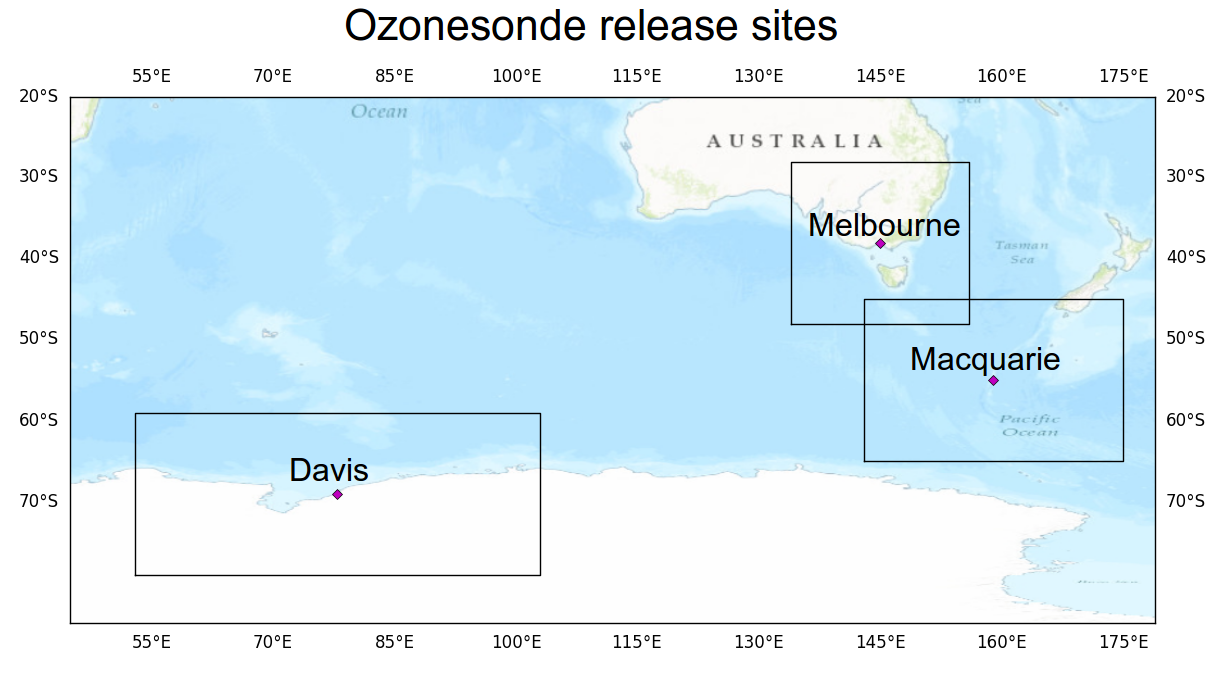
\includegraphics[width=10cm]{Figures/Ozone/ComparisonRegions.png}
      \caption{Ozonesonde release sites and the regions used to examine STT effect on tropospheric ozone levels.}
      \label{ch_StratOzone:fig:ComparisonRegion}
    \end{figure}
    
    Ozonesondes are launched approximately weekly from Melbourne (38$^{\circ}$ S, 145$^{\circ}$ E), Macquarie Island (55$^{\circ}$ S, 159$^{\circ}$ E) and Davis (69$^{\circ}$ S, 78$^{\circ}$ E), as shown in Fig. \ref{ch_StratOzone:fig:ComparisonRegion}. 
    Melbourne is a major city in the south east of Australia, and may be affected by anthropogenic pollution in the lower troposphere.
    Macquarie Island is isolated from the Australian mainland, situated in the remote Southern Ocean and unlikely to be affected by any local pollution events.
    Davis is on the coast of Antarctica and also unlikely to experience the effects of anthropogenic pollution.
    %Melbourne, a major city with more than 4 million residents \citep{ABS2016}, is in the far south eastern section of the Australian mainland.% Actual releases are north of the central business district in the Broadmeadows suburb.
    
    For this study, we use the 2004-2013 data for Melbourne and Macquarie Island and the 2006-2013 data for Davis because both ozone and geopotential height (GPH) are available from the World Ozone and Ultraviolet Data Centre archived data in these periods.
    At Davis, ozonesondes are launched twice as frequently during the ozone hole season and preceding months (June-October) as at other times of year \citep{Alexander2013}.
    A summary of ozonesonde releases at each site can be seen in Table \ref{ch_StratOzone:fig:sondesummary}.
    
    \begin{table}[t]
      \caption{Number of sonde releases at each site over the period of analysis.}
      \begin{tabular}{ c   c   c   c  } 
        \hline
        Site 		 & Total Releases & Monthly Releases (J, F, M, ...) & Date Range \\
        \hline
        Davis		 & 240	& 11, 12, 13, 12, 17, 31,	& 2006/04/13 -  \\ 
        &	& 29, 28, 32, 28, 15, 12 	& 2013/11/13	\\
        Macquarie Island & 390	& 32, 31, 45, 28, 34, 33,	& 2004/01/20 -  \\
        &	& 28, 35, 29, 33, 31, 31 	& 2013/01/09	\\ 
        Melbourne 	 & 456	& 31, 38, 40, 38, 41, 36,	& 2004/01/08 -  \\
        &	& 38, 39, 46, 40, 38, 31 	& 2013/12/18	\\
        \hline
      \end{tabular}
      \label{ch_StratOzone:fig:sondesummary}
    \end{table}
    
    Characterisation of STT events requires a clear definition of the tropopause.
    Two common tropopause height definitions are the standard lapse rate tropopause \citep{WMO1957} and the ozone tropopause \citep{Bethan1996}.
    The lapse rate tropopause is defined as the lowest altitude where the lapse rate (vertical gradient of temperature) is less than 2$^\circ$C~km$^{-1}$, provided the lapse rate averaged between this altitude and 2~km above is also below 2$^\circ$C~km$^{-1}$.
    The ozone tropopause is defined as the lowest altitude satisfying the following three conditions for the ozone mixing ratio (OMR) \citep{Bethan1996}:
    \begin{enumerate}
      \item Vertical gradient of OMR is greater than 60~ppb km$^{-1}$;
      \item OMR is greater than 80~ppb; and
      \item OMR exceeds 110~ppb between 500~m and 2000~m above the altitude under inspection (modified to between 500~m and 1500~m in the Antarctic, including the site at Davis).
    \end{enumerate}
    The ozone tropopause may misdiagnose the real tropopause altitude during stratosphere-troposphere exchange; however, it is useful at polar latitudes in winter, where the lapse-rate definition may result in artificially high values for tropopause height \citep{Bethan1996, Tomikawa2009, Alexander2013}.
    We require lapse rate defined tropopauses to be at a minimum of 4~km altitude. %This is due to several temperature inversions causing low misdiagnosed tropopauses.
    Another commonly used tropopause definition is determined with the use of PV (dynamical tropopause).
    In the extra-tropics the isosurface where PV$=2$~PVU (1~PVU$= 10^{-6}$~m$^2$ s$^{-1}$ K kg$^{-1}$) is often used to define the tropopause, allowing the 3D representation of tropopause folds and other tropopause features in a sufficiently resolved model \citep{Skerlak2014,Tyrlis2014}.
    The PV is not calculable using the ozonesonde measurements alone, so in this work the ozone tropopause is used when determining STT events or measured tropopause altitude.
    
    Figure \ref{ch_StratOzone:fig:seasonaltpheights} shows the monthly median ozone tropopause altitudes at each location (solid lines).
    At Melbourne, the tropopause altitude displays a seasonal cycle with maximum in summer and minimum is winter.
    This seasonality is missing at Macquarie Island and almost reversed at Davis, which has a minimum during autumn and maximum from winter to spring.
    Tropopause altitude decreases with latitude from 9-14 km at Melbourne (38$^\circ$ S) to 7-9 km at Davis (69$^\circ$ S).
    
    \begin{figure}[t] 
      % Figure 2
      % figure produced in seasonal_tropopause in Examine_stations.py
      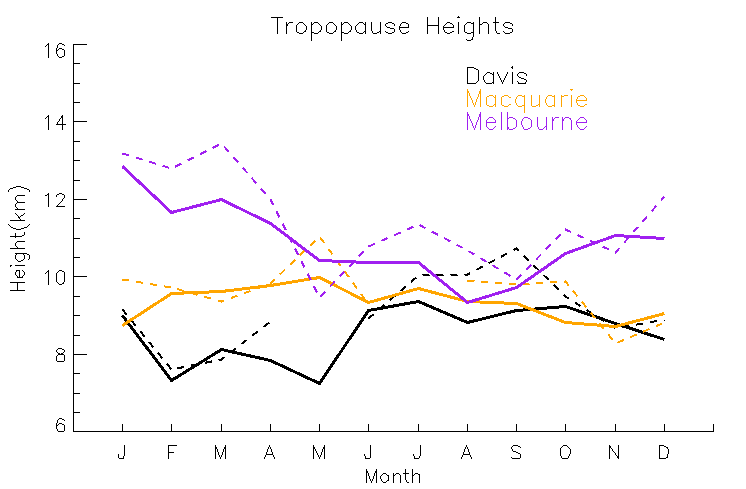
\includegraphics[width=10cm]{Figures/Ozone/tpheights.png}
      \caption{%
        Multi-year monthly median tropopause altitude (using the ozone defined tropopause) determined from ozonesondes measurements at Davis (2006-2013), Macquarie Island (2004-2013), and Melbourne (2004-2013) (solid lines).
        Dashed lines show the 10th to the 90th percentile of tropopause altitude for each site.}
      \label{ch_StratOzone:fig:seasonaltpheights}
    \end{figure}
  
    Figure \ref{ch_StratOzone:fig:seasonaltropozone} shows multi-year averaged ozone mixing ratios measured by ozonesonde over the three stations.
    Over Melbourne, increased ozone extending down through the troposphere is apparent from December to March and from September to November.
    The increased tropospheric ozone in these months is due to STT (in summer), and possible biomass burning influence (in spring), both discussed in more detail in the following sections.
    Over Davis and Macquarie Island, tropospheric ozone is higher between March and October, although the seasonal differences are small compared to those at Melbourne.
    %This seasonality at the high latitude sites is driven by a decrease in photochemical destruction under the reduced radiation conditions around polar night. % (TODO: read and cite S. Oltmans antarctic papers - re Andrews comment)... Can't find paper.
    The seasonality shown in Fig. \ref{ch_StratOzone:fig:seasonaltropozone} for Davis is consistent with remote free tropospheric photochemistry determined by solar radiation availability and temperature, resulting in higher ozone in winter \citep{Lelieveld2000}.
    NO$_2$ stratospheric observations have been conducted in the Southern hemisphere at Lauder, Macquarie Island and Arrival Heights \citep[i.e.][]{Struthers2004} which displays a winter minima in seasonality consistent with an ozone maxima.
    Influence from the ozone hole can be seen over Davis in October, with relatively low ozone levels extending up 5-6~km into the stratosphere.
    
    \begin{figure}[t]
      %Figure 3
      %Created by seasonal_tropozone function in examine_stations.py
      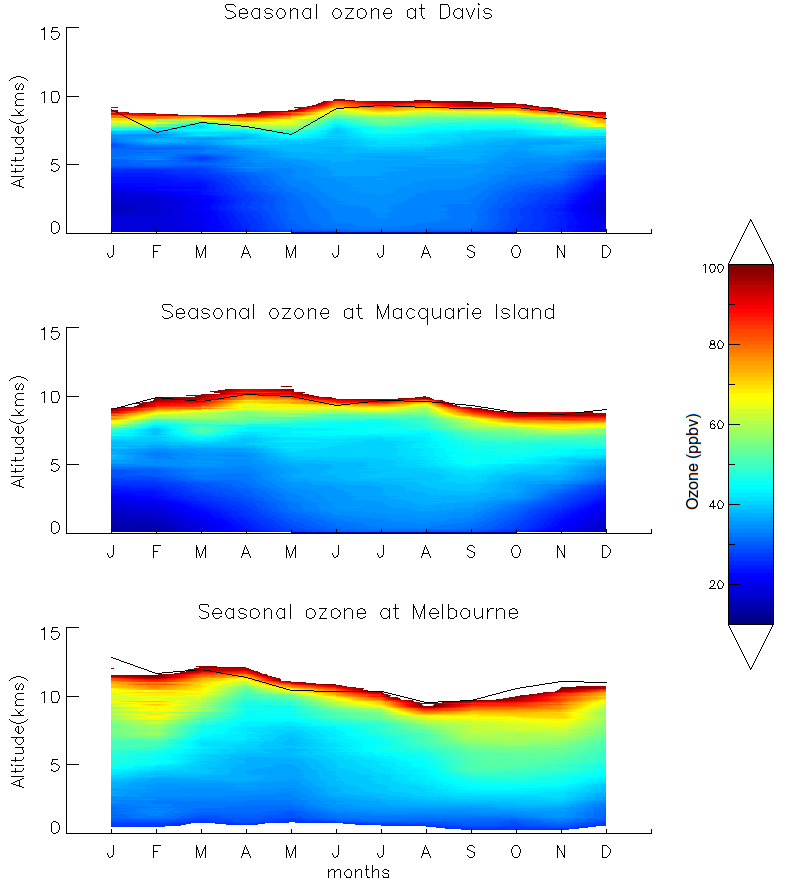
\includegraphics[width=12.0cm]{Figures/Ozone/seasonaltropozone}
      \caption{ %
        Multi-year mean seasonal cycle of ozone mixing ratio over Davis, Macquarie Island, and Melbourne as measured by ozonesondes.
        Measurements were interpolated to every 100~m and then binned monthly.
        Black and red solid lines show median ozone and lapse-rate defined tropopause altitudes (respectively), as defined in the text. }
      \label{ch_StratOzone:fig:seasonaltropozone}
    \end{figure}
  
  \subsection{Model description}
    \label{ch_StratOzone:sec:GEOSChemDescription}
    To provide regional and global context to the ozonesonde observations, we use the GEOS-Chem version 10-01 global chemical transport model \citep{Bey2001}, which simulates ozone along with more than 100 other trace gases throughout the troposphere and stratosphere. 
    Stratosphere-troposphere coupling is calculated using the stratospheric unified chemistry extension (UCX) \citep{Eastham2014}.
    Transport is driven by assimilated meteorological fields from the Goddard Earth Observing System (GEOS-5) maintained by the Global Modeling and Assimilation Office (GMAO) at NASA.
    Ozone precursor emissions are from the Model of Emissions of Gases and Aerosols from Nature (MEGAN) version 2.1 \citep{Guenther2012} for biogenic emissions, the Emissions Database for Global Atmospheric Research (EDGAR) version 4.2 for anthropogenic emissions, and the Global Fire Emissions Database (GFED4) inventory \citep{Giglio2013} for biomass burning emissions. 
    Our simulation was modified from the standard v10-01 to fix an error in the treatment of ozone data from the Total Ozone Mapping Spectrometer (TOMS) satellite used to calculate photolysis (see \url{http://wiki.seas.harvard.edu/geos-chem/index.php/FAST-JX_v7.0_photolysis_mechanism#Fix_for_TOMS_to_address_strange_cycle_in_OH_output.}).  
    
    Our simulations span 2005-2012 (following a 1-year spin-up) with horizontal resolution of 2$^{\circ}$ latitude by 2.5$^{\circ}$ longitude and 72 vertical levels from the surface to 0.01~hPa.
    The vertical resolution is finer near the surface at $\sim 60$~m between levels, spreading out to $\sim 500$~m near 10~km altitude.
    %, and reaching $\sim 1500$~m near the top of the atmosphere.
    For comparison to the ozonesonde observations, the model state was saved every 6 hours within the grid boxes containing each site.
    When comparing against ozonesondes, GEOS-Chem UTC+0 time samples are used for all sites.
    This means that the simulated ozone profiles are analysed at local times of 7AM for Davis, and 11AM for Macquarie Island and Melbourne.
    GEOS-Chem uses the tropopause height provided by GEOS-5 meteorological fields, which are calculated using a lapse-rate tropopause definition using the first minimum above the surface in the function $0.03 \times T(p) - \mathrm{log}(p)$, with p in hPa \citep{Rienecker2008}.
  
  \subsection{Characterisation of STT events and associated fluxes}
    \label{ch_StratOzone:sec:CharacterisationOfSTTs}
    
    We characterise STT events using the ozonesonde vertical profiles to identify tropospheric ozone enhancements above a local background (in moles per billion moles of dry air, referred to here as ppb).
    The process is illustrated in Figure~\ref{ch_StratOzone:fig:filterEG} on an example ozone profile.
    First, the ozone vertical profiles are linearly interpolated to a regular grid with 20~m resolution from the surface to 14~km altitude. 
    Small vertical-scale fluctuations in ozone, which are captured by the high-resolution ozonesondes, can be regarded as sinusoidal waves superimposed on the large vertical scale background tropospheric ozone.
    As such, the interpolated profiles are bandpass-filtered using a fast Fourier transform \citep{Press1992} to retain these small vertical scales, between 0.5~km and 5~km (removing low and high frequency perturbations).
    The high frequency perturbations are removed as they may represent noise in the measurements.
    The perturbations with scales longer than 5~km represent the vertical gradient of ozone concentration from the surface to the stratosphere.
    In what follows, these filtered vertical profiles are referred to as perturbation profiles.
    
    For an event to qualify as STT, a clear increase above the background ozone level is needed, as a bandpass filter leaves us with enhancements minus any noise or seasonal scale vertical profile effects.
    We next use all the perturbation profiles at each site to calculate the 95th percentile perturbation value for the site.
    The threshold is calculated from all the interpolated filtered values between 2~km above the surface and 1~km below the tropopause.
    This is our threshold for tropospheric ozone perturbations, and any profiles with perturbations exceeding this value in individual ozonesondes are classified as STT events.
    STT events at altitudes below 4~km are removed to avoid surface pollution, and events within 0.5~km of the tropopause are removed to avoid false positives induced by the sharp transition to stratospheric air.
    We note that this ozone detection methodology detailed above does not allow us to resolve STT events where the ozone flux is spread diffusely across the troposphere without a peak-like structure in the ozonesonde profile. 
    In other words, STT events which might have occurred some distance and time away from the location of the ozonesonde profiles may not be readily detected using the high vertical resolution, but infrequent, ozonesonde launches.
    
    \begin{figure}[t]
      % Figure 4 
      % created in getevents.pro, edited in inkscape
      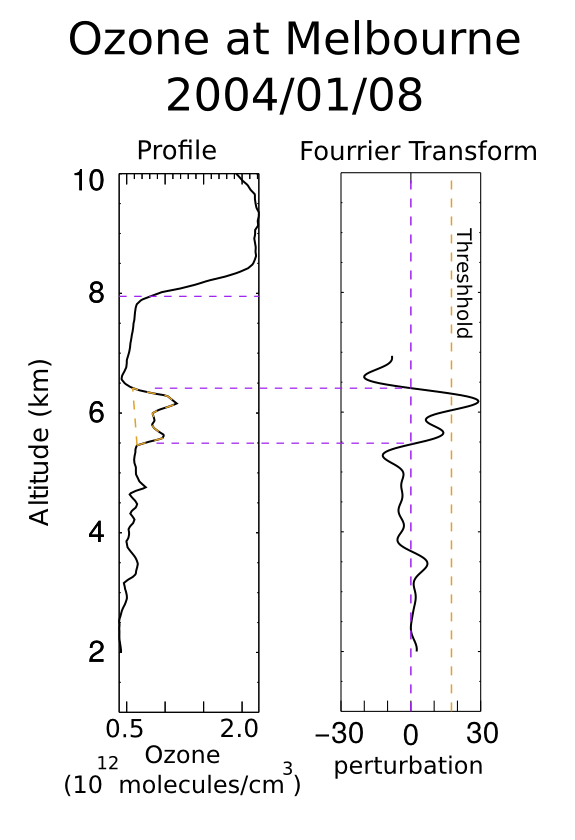
\includegraphics[width=8.3cm]{Figures/Ozone/filtereg.png}
      \caption{ %
        An example of the STT identification and flux estimation methods used in this work. 
        The left panel shows an ozone profile from Melbourne on 8 January 2004 from 2~km to the tropopause (blue dashed horizontal line).
        The right panel shows the perturbation profile created from bandpass filtering of the mixing ratio profile. The STT occurrence threshold calculated from the 95th percentile of all perturbation profiles is shown as the orange dashed line, and the vertical extent of the event is shown with the purple dashed lines (see details in text).
        The ozone flux associated with the STT event is calculated using the area outlined with the orange dashed line in the left panel.
      }
      \label{ch_StratOzone:fig:filterEG}
    \end{figure}
    
    We define the ozone peak as the altitude where the perturbation profile is greatest between 2~km from the surface and 0.5~km below the tropopause.
    The STT event is confirmed if the perturbation profile drops below zero between the ozone peak and the tropopause, as this represents a return to non-enhanced ozone concentrations.
    Alternatively, the STT event is also confirmed if the OMR between the ozone peak and the tropopause drops below 80~ppb and is at least 20~ppb lower than the OMR at the ozone peak. 
    If neither of these conditions are met, the profile is rejected as a non-event.
    This final step removes near-tropopause anomalies for which there is insufficient evidence of detachment from the stratosphere.
    Vertical ozone profiles recorded by ozonesondes are highly dependent on the time of launch \citep{Sprenger2003}, and it cannot be guaranteed that detected ozone enhancements are fully separated from the stratosphere, although this method minimises that risk by removing detected events too near the tropopause.
    
    We estimate the ozone flux into the troposphere associated with each event by integrating the ozone concentration enhancement vertically over the altitude range for which an STT event is identified (i.e. enhancement near the ozone peak over which the perturbation profile is greater than zero).
    This estimate is conservative because it does not take into account any ozone enhancements outside of the detected peak that may have been caused by the STT, and also ignores any enhanced ozone background amounts from synoptic-scale stratospheric mixing into the troposphere.
    
    Our method differs somewhat from that used by \citet{Tang2010} to detect STT events from ozonesonde measurements. 
    Their definition is based on subjective analysis of sondes released from 20 stations ranging in latitude from 35$^\circ$ S to 40$^\circ$ N.
    They identify an STT event if, starting from 5~km altitude, ozone exceeds 80~ppb and then within 3~km decreases by 20~ppb or more to a value less than 120~ppb.
    Their technique would miss many events due to the lower ozone concentrations found in the cleaner Southern Hemisphere.
  
  \subsection{Biomass burning influence}
    \label{ch_StratOzone:sec:BiomassBurning}
    The STT detection algorithm described in Sect. \ref{ch_StratOzone:sec:CharacterisationOfSTTs} assumes all ozone enhancements are caused by stratospheric intrusions.
    In some cases, however, these perturbations may in fact reflect ozone production in lofted smoke plumes.
    Biomass burning in southern Africa and South America has previously been shown to have a major influence on atmospheric composition in the vicinity of our measurement sites \citep{Oltmans2001, Gloudemans2006, Edwards2006}, particularly from July to December \citep{Pak2003, Liu2017}.
    %The downwind effects of biomass burning smoke plumes from South America and southern Africa are strongest around August and September, as seen here and in \citet{Liu2017}.
    On occasion, smoke plumes from Australian and Indonesian fires can also reach the mid-high southern latitudes, as seen from satellite measurements of carbon monoxide (CO) discussed below. %from the AIRS (Atmospheric Infrared Sounder) instrument on board the Aqua satellite \citep{AIRS3STD}.
    
    %Ozone precursors include nitrogen oxides ($NO_x = NO + NO_2$) and non methane volatile organic compounds (NMVOCs). % too basic for here..
    Large biomass burning events emit substantial quantities of ozone precursors, some of which are capable of being transported over long distances and driving ozone production far from the fire source \citep{Jaffe2012}.
    Ozone production from biomass burning is complex and affected by photochemistry, fuel nitrogen load, and time since emission, among other factors. 
    While ozone production occurs in some biomass burning plumes, this is not always the case; therefore ozone perturbations detected during transported smoke events may or may not be caused by the plume.
    For this reason all detected STT events which could be caused by smoke plumes are flagged, following the procedure outlined below.
    Calculations of seasonality, and ozone flux do not include flagged events, however they are included in summary plots in this work.
    
    %Biomass burning influence in the Southern Hemisphere comes mostly from Southern Africa and South America, however Australian fires from the midlatitudes, and Indonesian fires can also influence the ozonesonde release sites.
    %Transported biomass burning plumes influence the southern mid-latitudes generally between July and December \citep{Pak2003}.
    
    Possible biomass burning influence is identified using satellite observations of CO from the AIRS (Atmospheric Infra-red Sounder) instrument on board the Aqua satellite \citep{AIRS3STD}.
    CO is emitted during incomplete combustion and is an effective tracer of long-range transport due to its long lifetime \citep{Edwards2003, Edwards2006}.
    In the Southern Hemisphere, biomass burning is the primary source of CO, making CO a good proxy for fire plumes \citep[e.g.][]{Sinha2004, Mari2008}.
    To identify possible biomass burning influence, AIRS vertical column CO is visually inspected for all dates with detected STT events.
    Smoke plumes are diagnosed over areas with elevated CO columns ($\sim 2 \times 10^{18}$ molecules cm$^{-2}$ or higher), and any sonde-detected STT event that occurs near (within $\sim$150~km of) a smoke plume is flagged.
    Removal of these detections reduces the yearly estimated ozone flux by $\sim 15\%$ at Macquarie Island and $\sim 20\%$ at Melbourne.
    
    All days with detected STT events were screened, with the exception of one event during which there were no available AIRS data (January 2010).
    We find that biomass burning may have influenced 27 events over Melbourne and 21 events over Macquarie Island.
    These events are flagged in the following sections, and are not used in our calculation of total STT flux.
    All of the flagged events except for two occurred during the SH burning season (July to December). %\citet{Edwards2006}). % burning season from \citep{Pak2003}.
    No events at Davis were seen to be influenced by smoke transport.
  
  \subsection{Classifying synoptic conditions during STT events}
    \label{ch_StratOzone:sec:WeatherClassifications}
    Synoptic scale weather patterns are examined using data from the European Centre for Medium-range Weather Forecasts (ECMWF) Interim Reanalysis (ERA-I) \citep{Dee2011}.
    This is done using the ERA-I data products over the three sites on dates matching the detected STT events.
    We use the ERA-I 500~hPa data to subjectively classify the events based on their likely meteorological cause, by visually examining each date where an event was detected.
    During STT occurrence, the upper troposphere is typically characterised by nearby cyclones, cut-off lows, or cold fronts.
    Over Melbourne and Macquarie Island, we find that frontal and low pressure activity are prevalent during STT events (see Sect. \ref{ch_StratOzone:sec:eventclimatologies}).
    Over Davis, the weather systems are often less clear, however we see a higher portion of probable cut-off lows. 
    The stratospheric polar vortex may create tropopause folds without other sources of upper tropospheric turbulence such as low pressure fronts or cyclones \citep[e.g.][]{Baray2000,Sprenger2003,Tyrlis2014}.
    %, for example near the more intense part of the subtropical jet over the Middle East \citep{Tyrlis2014}.
    Cut-off low pressure systems can be seen clearly in synoptic scale weather maps as regions with lowered pressure and cyclonic winds.
    Low pressure fronts in the higher southern latitudes travel from west to east and lower the tropopause height.
    We examine two cases in detail to illustrate the relationship between synoptic-scale conditions and STT events over Melbourne.
    These are included in a supplementary document (Fig. S2 and S3) which show an archetypal cut-off low and low pressure front.
    To detect cut-off low pressure systems we look for cyclonic winds and a detached area of low pressure within $\sim 500$~km of a site on days of event detection.
    For low pressure fronts we look for low pressure troughs within $\sim 500$~km.
    Frontal passage is a known cause of STT as stratospheric air descends and streamers of ozone-rich air break off and mix into the troposphere \citep{Sprenger2003}.


\section{STT event climatologies}
  \label{ch_StratOzone:sec:eventclimatologies}
  Figure \ref{ch_StratOzone:fig:SummarySeasonality} shows the seasonal cycles of STT frequency at Davis, Macquarie Island, and Melbourne.
  Frequency is determined as detected event count divided by total launched ozonesondes for each month.
  STT events in Figures \ref{ch_StratOzone:fig:SummarySeasonality}-\ref{ch_StratOzone:fig:SummaryTPDepths} are coloured based on the meteorological classification described in Sect. \ref{ch_StratOzone:sec:WeatherClassifications}, with events classified as either low pressure fronts (“frontal”, dark blue), cut-off low pressure systems (“cutoff”, teal), or indeterminate (“misc”, cyan).
  Events that may have been influenced by transported smoke plumes (Sect. \ref{ch_StratOzone:sec:BiomassBurning}) are shown in red.
  Ozonesonde releases are summarised in Table \ref{ch_StratOzone:fig:sondesummary} and detected event counts are summarised in Table \ref{ch_StratOzone:fig:EventCounts}.
  \begin{table}[t]
    %\centering
    \caption{Total number of ozonesonde detected STT events, along with the number of events in each category (see text).}
    \begin{tabular}{ c   c   c   c   c   c   c } 
      \hline
      Site & Events & Cut-offs & Frontals & Misc & Fire \\
      \hline
      % 41,   31,  28,  27
      Davis       	& 80 & 44  & 19 & 17 & 0 \\ 
      Macquarie Island 	& 105 & 19 & 31 & 34  & 21 \\
      Melbourne 	& 127 & 28 & 31 & 41 & 27 \\
      \hline
    \end{tabular}
    \label{ch_StratOzone:fig:EventCounts}
  \end{table}
  
  \begin{figure}[t]
    % these IMAGE CREATED BY non_transport_summary.py, labels edited IN INKSCAPE
    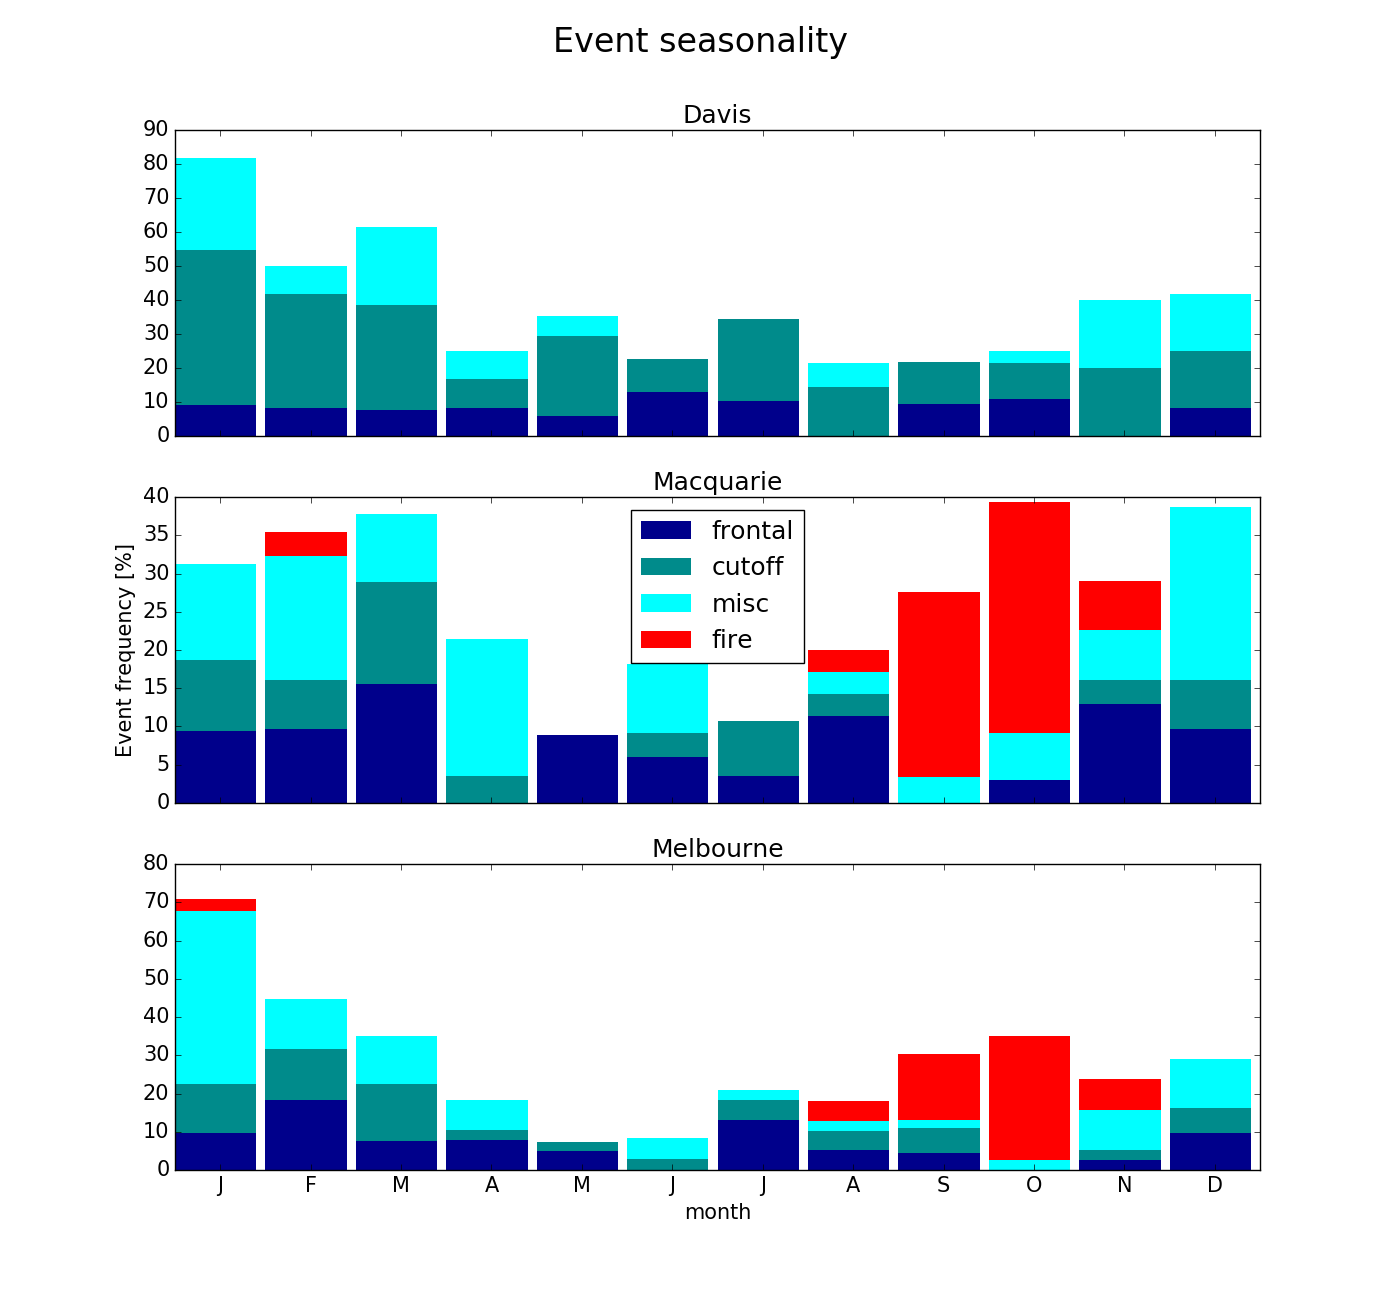
\includegraphics[width=12cm]{Figures/Ozone/summary_season.png}
    \caption{Seasonal cycle of STT event frequency at Davis (top), Macquarie Island (middle), and Melbourne (bottom).
      Events are categorised by associated meteorological conditions as described in the text, with low pressure fronts (“frontal”) in dark blue, cut-off low pressure systems (“cutoff”) in teal, and indeterminate meteorology (“misc”) in cyan. 
      Events that may have been influenced by transported smoke plumes are shown in red (see text for details).}
    \label{ch_StratOzone:fig:SummarySeasonality}
  \end{figure}
  
  There is an annual cycle in the frequency of STT events  (Fig. \ref{ch_StratOzone:fig:SummarySeasonality}) with a summertime peak at all three sites.
  This summertime peak is due to a prevalence of summer low-pressure storms and fronts, which increase turbulence and lower the tropopause \citep{Reutter2015}.
  At Davis, there are more STT detections during winter relative to our other sites, which may be due to the polar vortex and its associated lowered tropopause and increased turbulence.
  STT events associated with cut-off low pressure systems are more prevalent during summer, while STT events associated with frontal passage occur throughout the year.
  The high frequency of STT ozone enhancements is comparable to the $>25\%$ frequencies seen over Turkey and east of the Caspian sea in an ERA-I analysis performed by \citet{Tyrlis2014}. 
  
  The SH summer maximum we see for STT ozone flux can also be seen in Fig. 16 of \cite{Skerlak2014}, which shows seasonal flux over the southern ocean, although this is less clear over Melbourne.
  This seasonality is not clear in the recent ERA-Interim tropopause fold analysis performed by \citet{Skerlak2015}, where a winter maximum of tropopause fold frequency ($\sim 0.5\%$ more folds in winter) over Australia can be seen to the north of Melbourne.
  Their work seems to show slightly higher fold frequencies over Melbourne in summer \citep[][Fig. 5]{Skerlak2015}, however not to the same extent that our summer peak suggests.
  Their winter maximum is in the subtropics only - from around 20$^{\circ}$~S to 40$^{\circ}$~S, which can be seen as the prevalent feature over Australia in their Fig. 5.
  \cite{Wauben1998} look at modelled (CTM driven by ECMWF output) and measured ozone distributions and find more SH ozone in the lower troposphere during austral winter, however they note that the ECMWF fields are uncertain here again due to lack of measurements.
  Their work shows a generally cleaner lower troposphere in the SH summer but this can not be construed to suggest more or less STT folds in either season.
  \cite{Sprenger2003} examine modelled STT folds using ECMWF output over March 2000 - April 2001, and show that for this year there is a clear austral winter maximum, again over the 20$^{\circ}$~S to 40$^{\circ}$~S band.
  The winter maximum does not include Melbourne, or the southern ocean, which explains why we see a seasonality not readily evident in these global-scale studies.
  
  The measurement sites are not in the regions which have a clear winter maximum seen in \cite[Fig. 1][]{Sprenger2003}, and the large scale winter maximum shown by all three studies seems to be dominated by the system in that region.
  The seasonality of our three sites is not driven by the larger STT system seen over the southern Indian ocean and middle Australia which dominates prior analysis near or over Australia.
  
  To examine the robustness of the distributions shown in Fig. \ref{ch_StratOzone:fig:SummarySeasonality}, we developed an alternative assessment of the seasonal occurrence of STT events, with results shown in Fig. \ref{ch_StratOzone:fig:AndrewProxySTT}.
  Here STT occurrence is evaluated by consideration of the square of the dry Brunt-V\"{a}is\"{a}l\"{a} frequency (N$^2$) at the heights of the ozone tropopause (z$_{OT}$) and lapse rate tropopause (z$_{LRT}$) in each ozonesonde profile that has been binned to 100~m resolution.
  We use N$^2$ to assess atmospheric stability, which is normally distinctly higher in the stratosphere than in the troposphere, and assume that the vertical temperature gradients within the intrusion respond most rapidly to transported heat, which is an additional characteristic of stratospheric air.
  N$^2$ is evaluated using 250~m resolution data (to smooth variability in the vertical gradient of potential temperature that is due to small temperature fluctuations likely associated with gravity waves).
  The altitude binning chosen is a compromise between vertical resolution and the level of variability in N$^2$ introduced by temperature gradients associated with perturbations from gravity waves and changes near the lapse rate tropopause, and is the minimum that produces a robust seasonal distribution.
  We define STT as having taken place if N$^2$(z$_{OT}$) $>$ N$^2$(z$_{LRT}$) and z$_{OT}$ $<$ z$_{LRT}$; in this way the characteristically higher static stability and ozone concentration of stratospheric intrusion is regarded as being retained as it penetrates below the lapse rate tropopause. 
  The seasonal distributions shown for the three stations in Fig. \ref{ch_StratOzone:fig:AndrewProxySTT} are generally similar to those shown in Fig. \ref{ch_StratOzone:fig:SummarySeasonality} (although detected events are less frequent), with the main exception that very few events are identified with the alternative method at Davis in the first half of the year.
  For our STT proxy, we only detect intrusions where the lowest altitude of the intrusion satisfies the ozone tropopause definition. During summer and autumn, the vertical ozone gradients at Davis are weaker compared with the other seasons, and the detected ozone tropopause tends to lie above the lapse rate tropopause potentially reducing the ability to identify STT events based on the definition of our proxy.
  
  \begin{figure}[t]
    % Figure from Andrew Klekociuk data, plotted in examinestations.py
    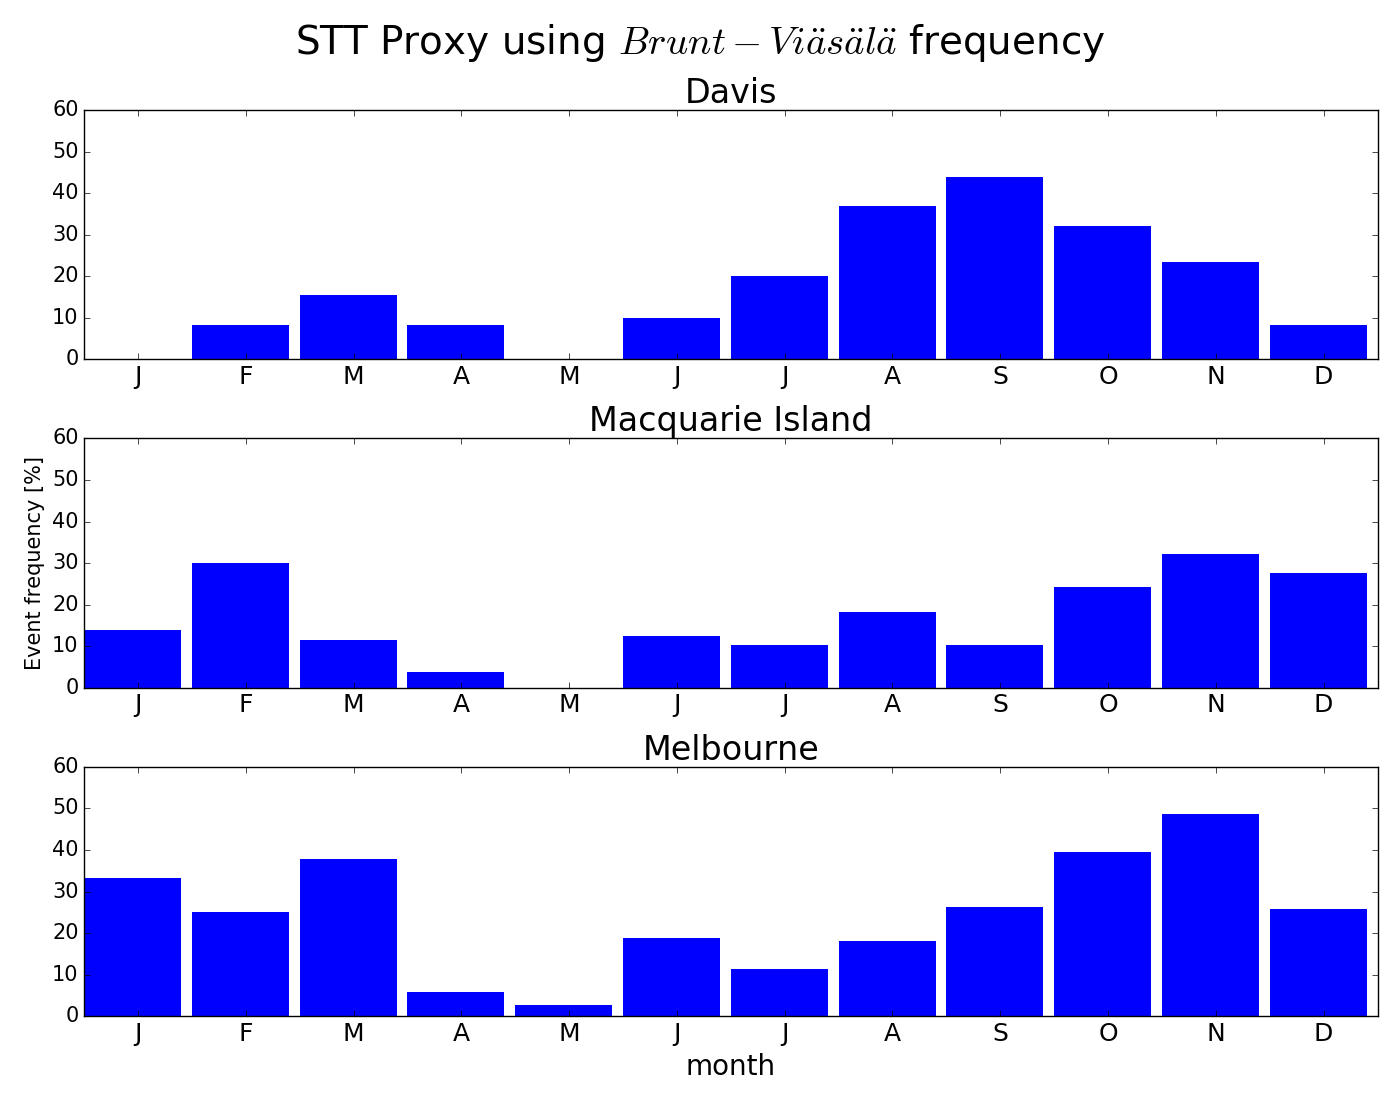
\includegraphics[width=10cm]{Figures/Ozone/AndrewProxySTTV2.png}
    \caption{Seasonal distribution of STT events using the alternative STT proxy, obtained from consideration of the static stability at the ozone and lapse rate tropopauses, for Davis (2006-2013), Macquarie Island (2004-2013), and Melbourne (2004-2013).}
    \label{ch_StratOzone:fig:AndrewProxySTT}
  \end{figure}
  
  Figure \ref{ch_StratOzone:fig:SummaryAltitudes} shows the altitudes of detected events, based on the altitude of peak tropospheric ozone (local maximum ozone within enhancement altitude) in the ozonesonde profile.
  STT event peaks most commonly occur at 6--11~km above Melbourne and anywhere from 4--9~km at Davis and Macquarie Island.
  There is no clear relationship between meteorological conditions and event altitude, which may reflect the fact that the ozonesondes observe a snapshot of an event at different stages of its life cycle.
  
  \begin{figure}[t]
    % fig 7
    % done in examine_stations I think
    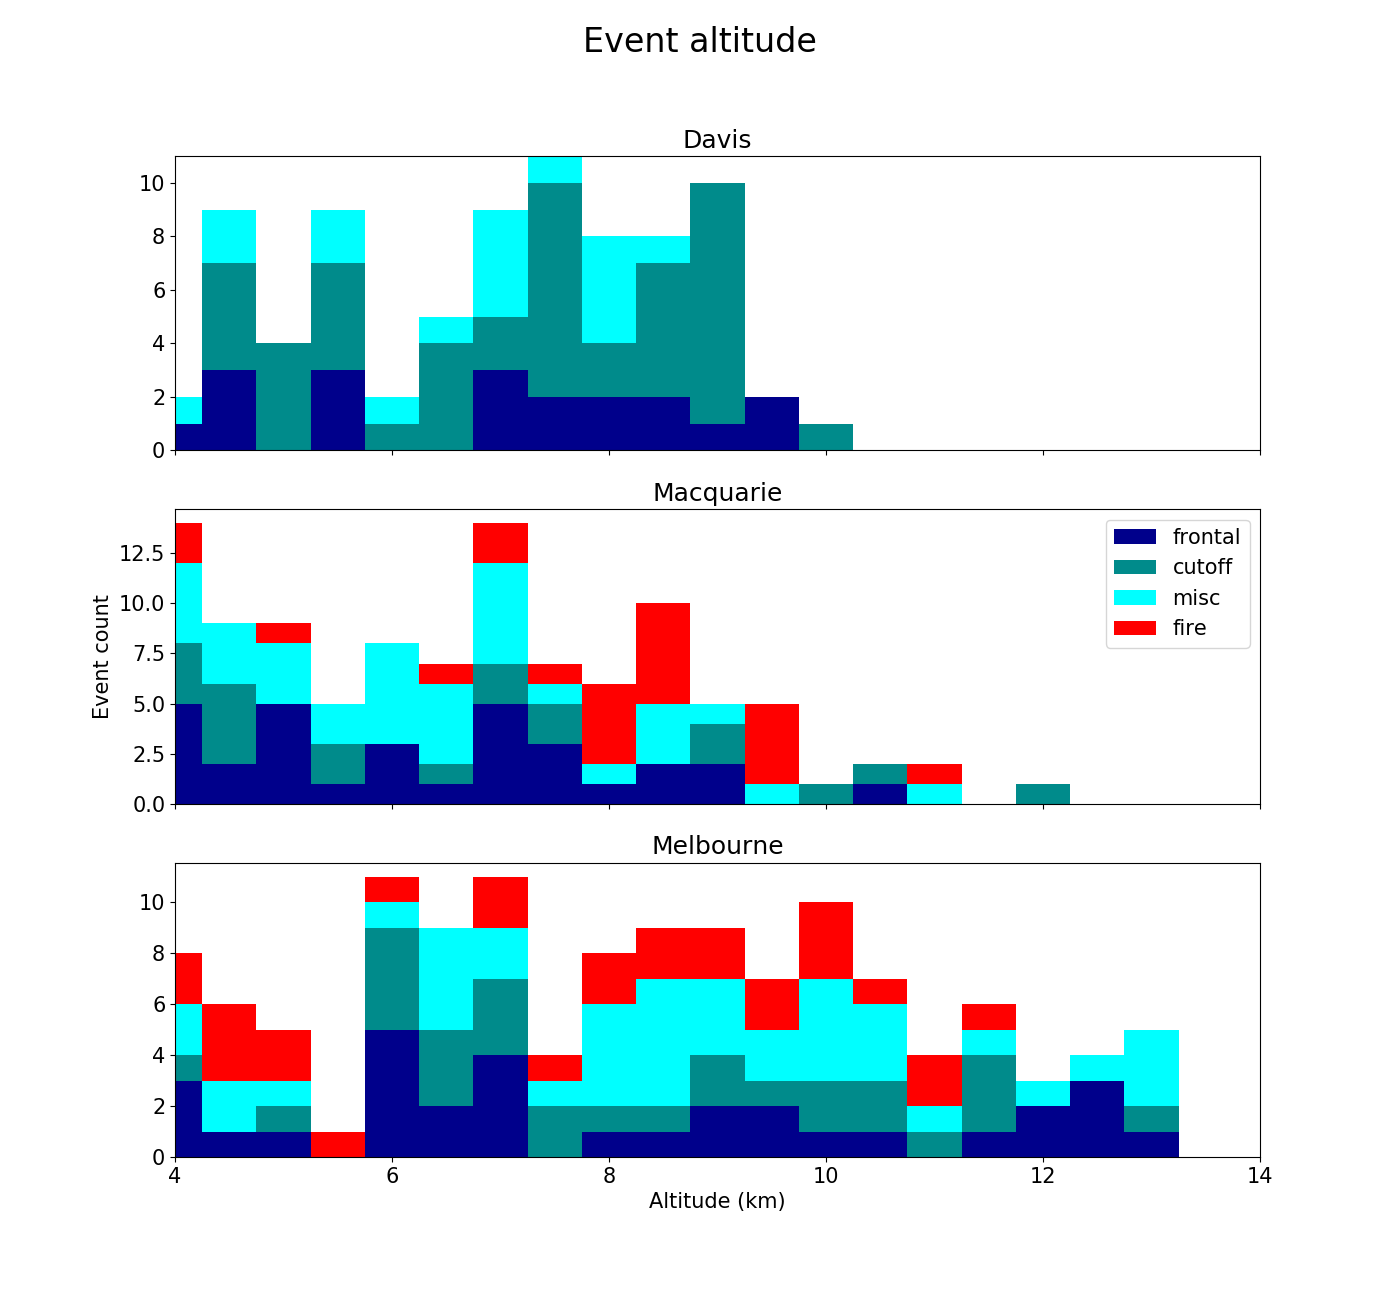
\includegraphics[width=12cm]{Figures/Ozone/summary_altitude.png}
    \caption{The distribution of STT events' altitudes at Davis (top), Macquarie Island (middle), and Melbourne (bottom), determined as described in the text.
      Events are coloured as described in Fig. \ref{ch_StratOzone:fig:SummarySeasonality}.}
    \label{ch_StratOzone:fig:SummaryAltitudes}
  \end{figure}
  
  Figure \ref{ch_StratOzone:fig:SummaryTPDepths} shows the distance from the event peak to the ozone defined tropopause, referred to as event depth.
  The majority of STT events occur within 2.5~km of the tropopause at Davis and Macquarie Island. 
  Over Melbourne, the event depth is more spread out, with peak ozone enhancement generally occurring up to 6~km below the tropopause.
  Again, there is no clear relationships between meteorological conditions and event depth.
  
  \begin{figure}[t]
    % Fig 8
    % 
    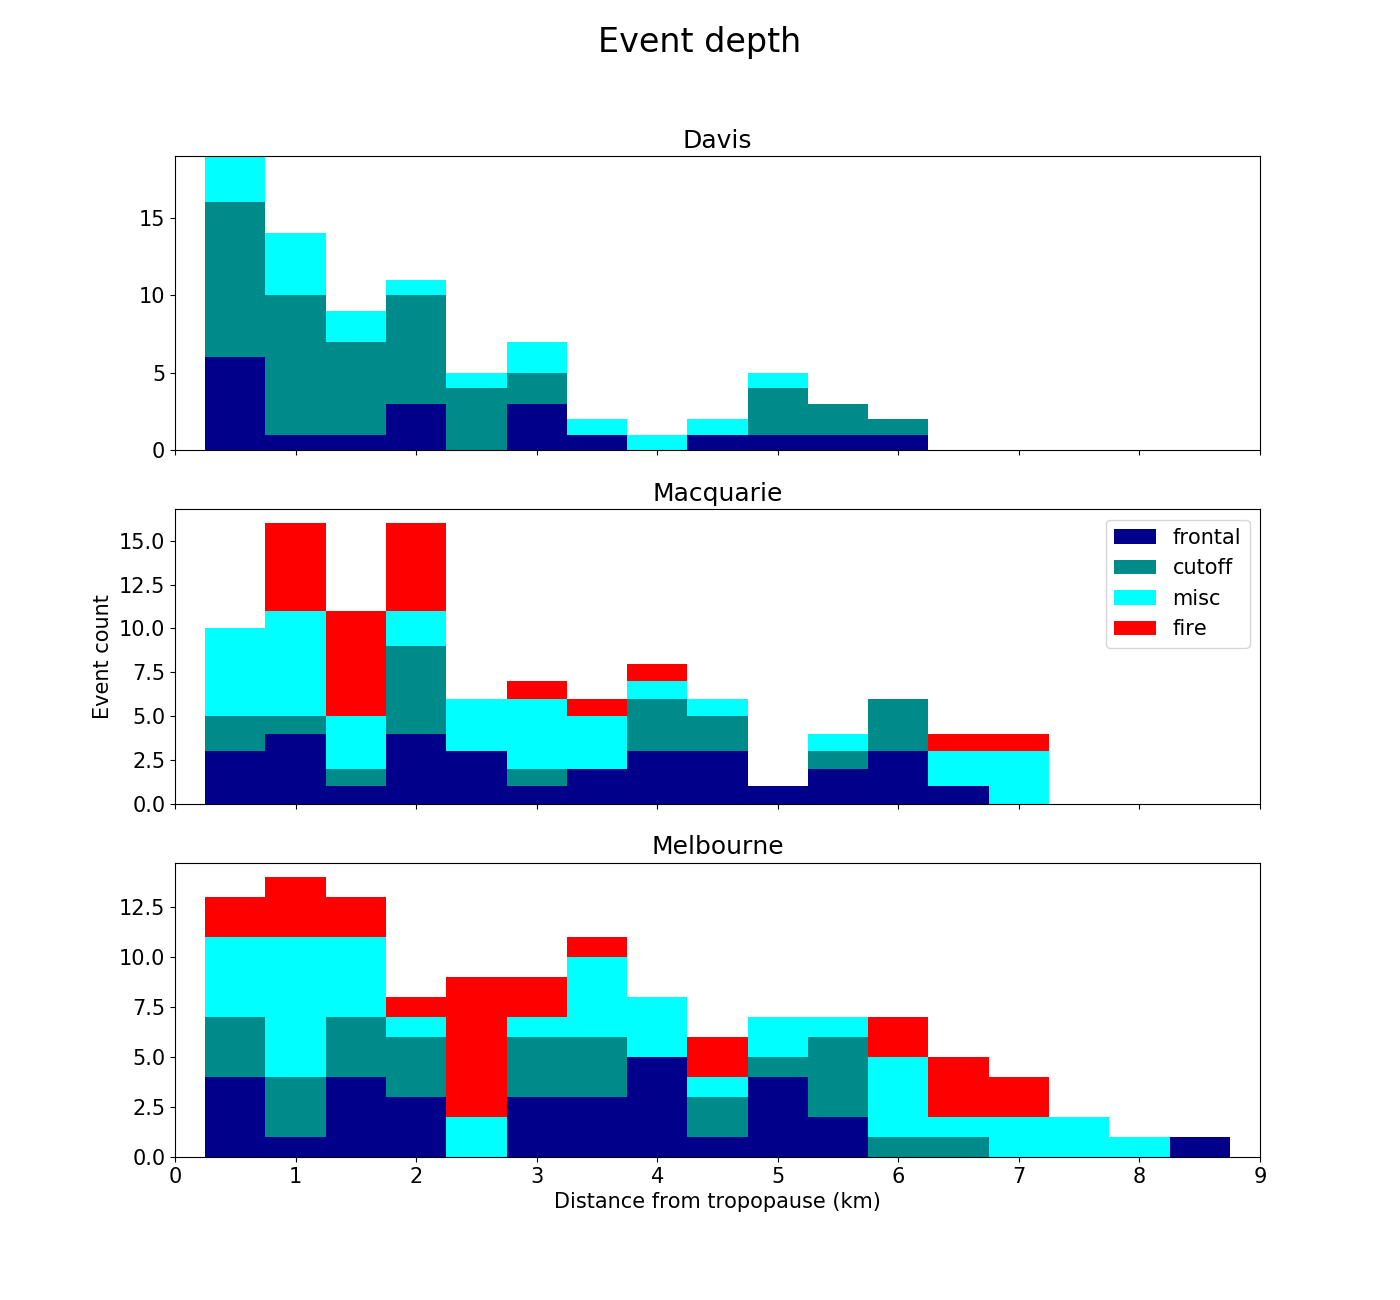
\includegraphics[width=12cm]{Figures/Ozone/summary_depth.png}
    \caption{The distribution of STT events' depths, defined as the distance from the event to the tropopause, at Davis (top), Macquarie Island (middle), and Melbourne (bottom), determined as described in the text.
      Events are coloured as described in Fig. \ref{ch_StratOzone:fig:SummarySeasonality}.}
    \label{ch_StratOzone:fig:SummaryTPDepths}    
  \end{figure}
  
\section{Simulated ozone columns}
  \label{ch_StratOzone:sec:ModelComparison}
  Figure \ref{ch_StratOzone:fig:StationSeriesGEOSChem} compares the time series of tropospheric ozone columns ($\Omega_{O_3}$) in molecules cm$^{-2}$ simulated by GEOS-Chem (red) to the measured tropospheric ozone columns (black).
  GEOS-Chem outputs ozone density (molecules cm$^{-3}$), and height of each simulated box, as well as which level contains the tropopause, allowing modelled $\Omega_{O_3}$ to be calculated as the product of density and height summed up to the box below the tropopause level.
  In both observations and model, the maximum ozone column at Melbourne occurs in austral summer, with a minimum in winter, while Macquarie Island and Davis show the opposite seasonality.
  
  \begin{figure}
    % made in examine_stations.py in stations repository
    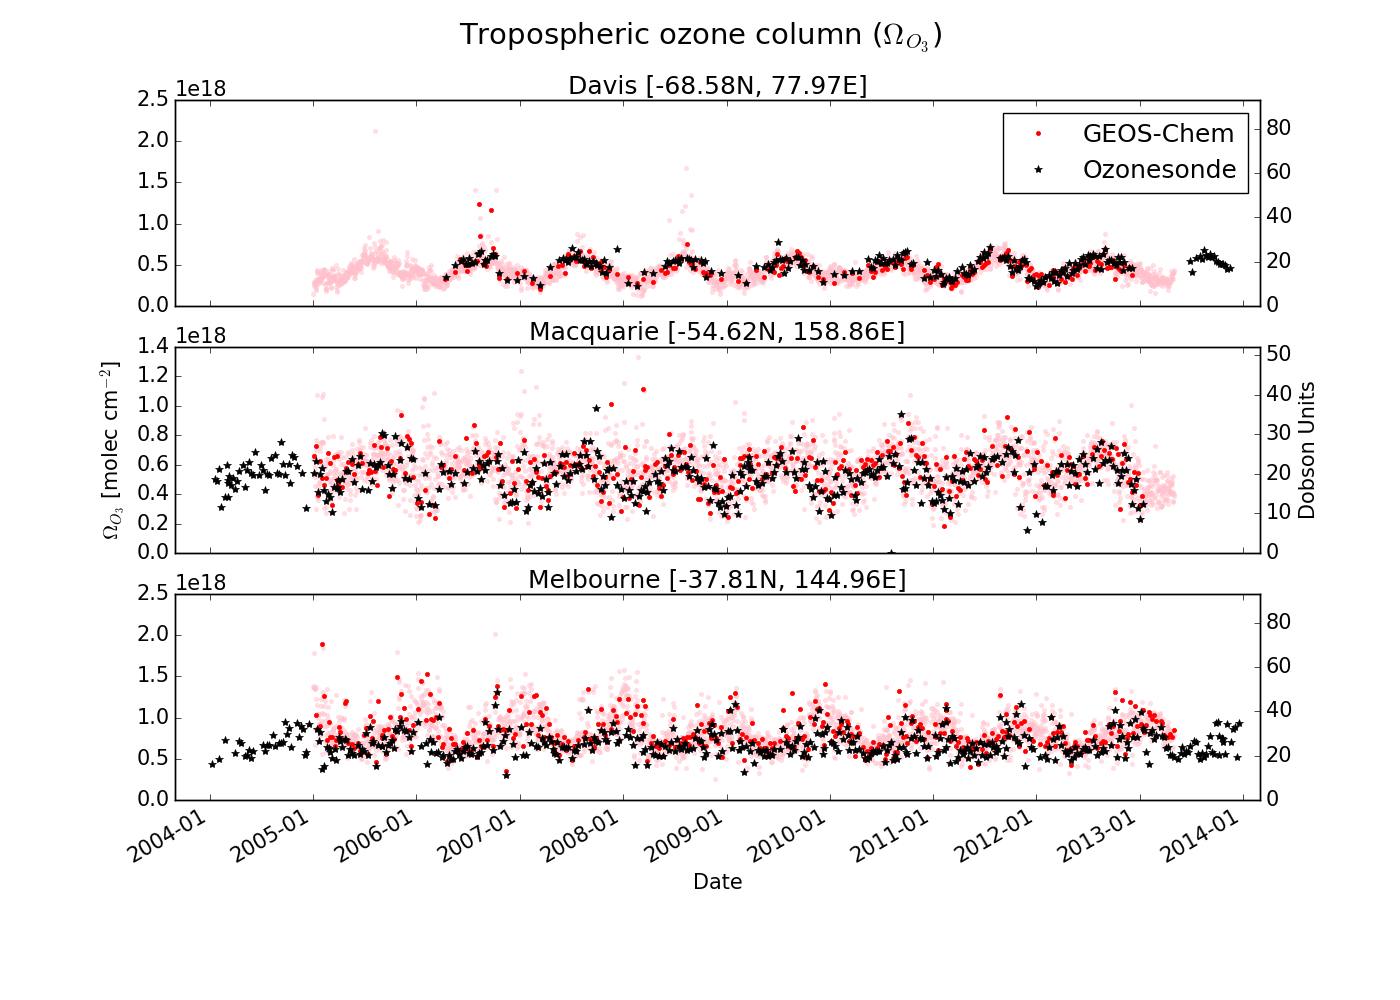
\includegraphics[width=12.0cm]{Figures/Ozone/StationSeries.png}
    \caption{Comparison between observed (black) and simulated (pink, red) tropospheric ozone columns ($\Omega_{O3}$, in molecules cm$^{-2}$) from 1 January 2004 to 30 April 2013.
      For the model, daily output is shown in pink, while output from days with ozonesonde measurements are shown in red.
      For each site, the model has been sampled in the relevant grid square.}
    \label{ch_StratOzone:fig:StationSeriesGEOSChem}
  \end{figure}
  
  GEOS-Chem provides a reasonable simulation of the observed seasonality and magnitude of $\Omega_{O_3}$.
  Reduced major axis regression of observed versus simulated $\Omega_{O_3}$ gives a line of best fit with slopes of 1.08 for Davis, 0.99 for Macquarie Island, and 1.34 for Melbourne.
  The model is only partially able to reproduce the variability in the observations, with paired r$^2$ values of 0.38 for Davis, 0.18 for Macquarie Island, and 0.37 for Melbourne.
  Much of the variability is driven by the seasonal cycle, and after removing this effect (by subtracting the multi-year monthly means), the r$^2$ values decrease to 0.07, 0.11, and 0.30 respectively, although the slope improves at Melbourne to 1.08.
  %The model shows more day-to-day variability than the ozonesondes (MAYBEDO: Verify this), although there are daily simulated values for the model while only weekly or less for the ozonesondes.
  
  \begin{figure}
    % Created in examine_stations.py
    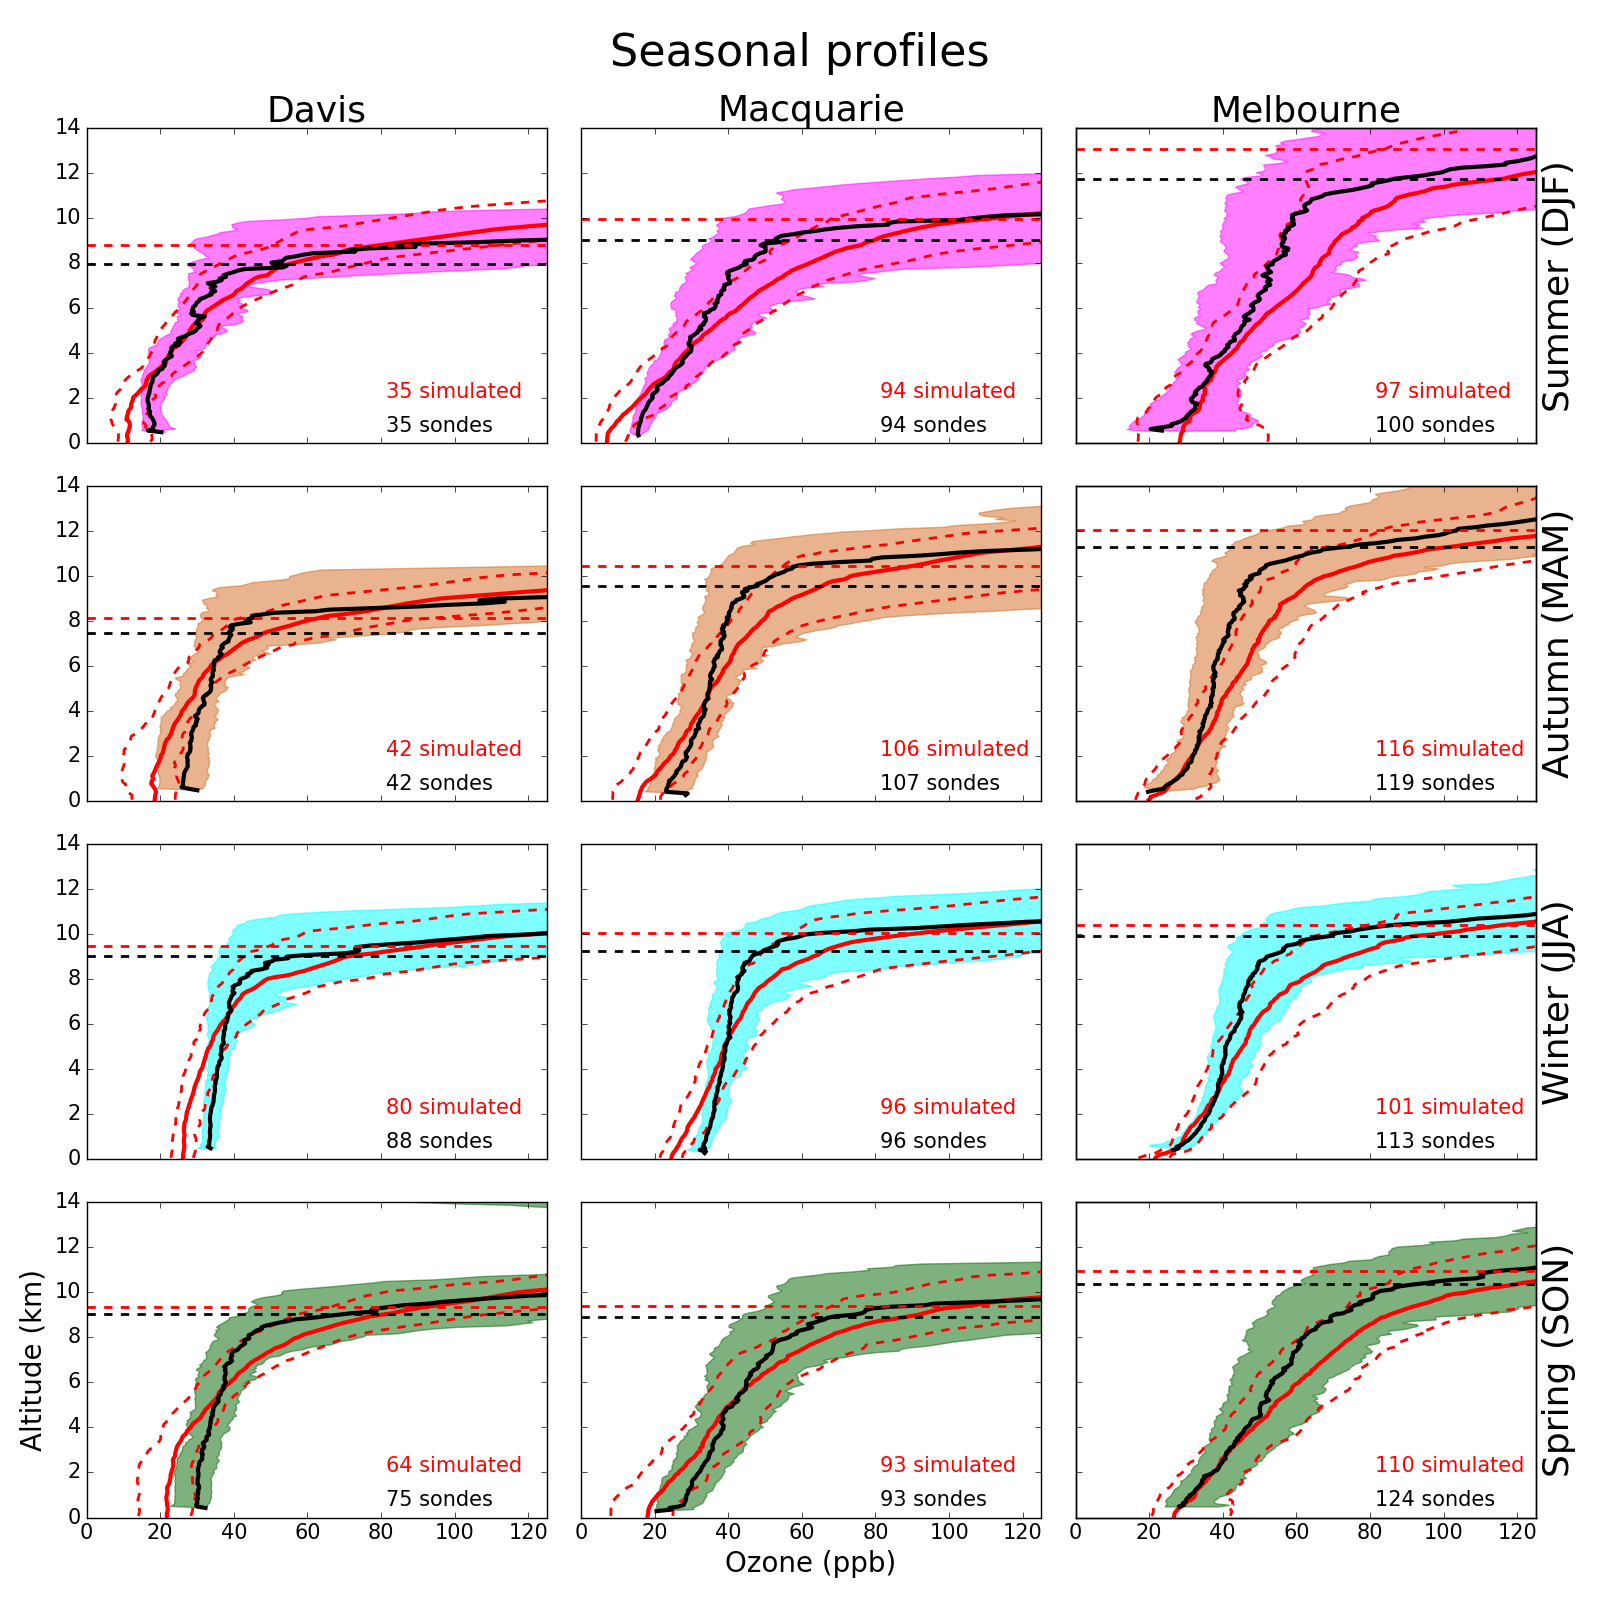
\includegraphics[width=14.0cm]{Figures/Ozone/seasonalprofiles00.png}
    \caption{%
      Observed and simulated tropospheric ozone profiles over Davis, Macquarie Island, and Melbourne, averaged seasonally.
      Model medians (2005-2013 average) are shown as red solid lines, with red dashed lines showing the 10th and 90th percentiles.
      Ozonesonde medians (over each season, for all years) are shown as black solid lines, with coloured shaded areas showing the 10th and 90th percentiles.
      The horizontal dashed lines show the median tropopause heights from the model (red) and the observations (black).}
    \label{ch_StratOzone:fig:GEOSChemSeasonalProfiles}
  \end{figure}
  
  Figure \ref{ch_StratOzone:fig:GEOSChemSeasonalProfiles} shows the observed and simulated ozone profiles at all sites, averaged seasonally.
  The model generally underestimates ozone in the lower troposphere (up to 6~km) over Davis, although this bias is less pronounced during summer.
  Over Melbourne, ozone in the lower troposphere is well represented, but the model overestimates ozone from around 4~km to the tropopause.
  Over Macquarie Island we see model overestimation of ozone above 4~km, as well as underestimated ozone in the lower troposphere, suggesting that this region is influenced by processes seen at both of our other sites.
  Also shown is the mean tropopause height simulated by the model (horizontal dashed red line), which is always higher than the observed average, although this difference is not statistically significant.
  The effect of local pollution over Melbourne during austral summer (DJF) can be seen from the increased mean mixing ratios and enhanced variance near the surface.
  The gradient of the O$_3$ profiles is steeper in the measurements than the model, at all sites during all seasons.
  Recently \cite{Hu2017} examined GEOS-Chem ozone simulations and found a similar overestimation of upper troposphere ozone in the mid southern latitudes when using the GEOS5 meteorological fields.
  
  Figure \ref{ch_StratOzone:fig:event_profile_comparison} compares modeled (red) and observed (black) ozone profiles on three example days when STT events were detected using the ozonesondes. 
  The figures show the profile for each site with the closest (qualitative) match between model and observations.
  The resolution (both vertical and horizontal) of GEOS-Chem in the upper troposphere is too low to consistently allow detection of STTs, although in a few cases (e.g., Melbourne in Fig. \ref{ch_StratOzone:fig:event_profile_comparison}) it appears that the event was large enough to be visible in the model output.
  
  \begin{figure}
    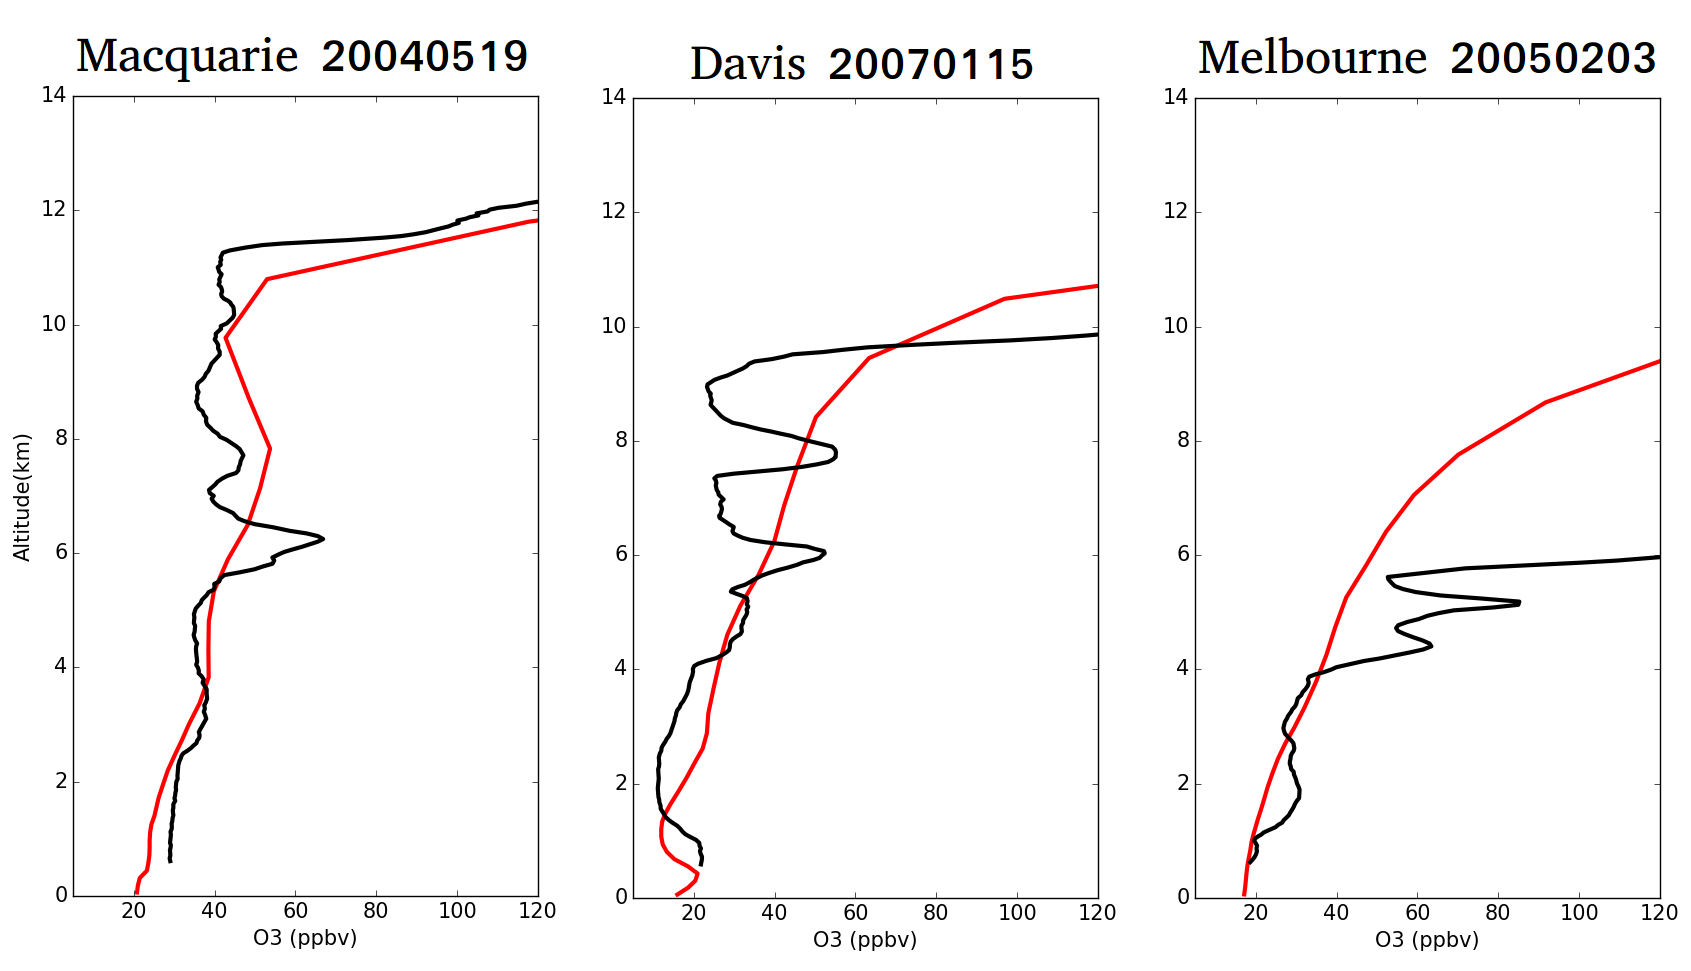
\includegraphics[width=12cm]{Figures/Ozone/event_profile_comparison.png}
    \caption{%
      Example comparisons of ozone profiles from ozonesondes (black) and GEOS-Chem (red) from three different dates during which STT events were detected from the measurements.
      The dates were picked based on subjective visual analysis. 
      The examples show the best match between model and observations for each site.
      GEOS-Chem and ozonesonde pressure levels are marked with red and black dashes respectively.}
    \label{ch_StratOzone:fig:event_profile_comparison}
  \end{figure}
  
\section{Stratosphere-to-troposphere ozone flux from STT events}
  \label{ch_StratOzone:sec:STTevents}
  
  \subsection{Method}
    \label{ch_StratOzone:sec:fluxcalc}
    We quantify the mean stratosphere-to-troposphere ozone flux due to STT events at each site based on the integrated ozone amount associated with each STT event (see Sect. \ref{ch_StratOzone:sec:CharacterisationOfSTTs}).
    Events that may have been influenced by transported biomass burning are excluded from this calculation.
    Our estimate provides a preliminary estimate of how much ozone is transported from the stratosphere by the events detected by our method.
    The estimate is conservative for several reasons: it ignores secondary ozone peaks which may also be transported from the stratosphere, it ignores potential ozone enhancements which may have dispersed and increased the local background mixing ratio, and any influence from STT events nearby which may also increase the local background ozone.
    
    Observed tropospheric columns are calculated from the ozonesondes by calculating the ozone number density (molecules cm$^{-3}$) using measured ozone partial pressure (P$_{O_3}$) and integrating vertically up to the tropopause:
    % Using \begin{equation*}... doesn't center the equation so I've used $$ instead.
    \begin{equation*} \Omega_{O_3} = \int_{0}^{TP} \frac{P_{O_3}(z)}{k_B \times T(z)} \mathrm{d}z \end{equation*}
    where $z$ is the altitude (GPH), $TP$ is the altitude at the tropopause, $T$ is the temperature, and $k_B$ is the Boltzmann constant.
    
    Three regions are used to examine possible STT flux over a larger area using modeled tropospheric ozone concentrations.
    The regions are shown in Fig. \ref{ch_StratOzone:fig:ComparisonRegion}.
    The regions are centred at each site, plus or minus ten degrees latitude, and plus or minus 25, 16, and 11 degrees longitude for Davis, Macquarie Island, and Melbourne respectively.
    These boundaries approximate a rectangle centred at each site with $\sim 2000$~km side lengths, covering $\sim 4.4$, $4.6$, and $4.8$ million square km, for Davis, Macquarie Island, and Melbourne respectively.
    
    To determine the ozone column attributable to STT, we determine monthly averaged STT impact (\textit{I}; fraction of tropospheric ozone sourced from the stratosphere as shown above) and the monthly mean tropospheric ozone column (from the GEOS-Chem multi-year mean, $\Omega_{O_3}$) over the regions described above.
    This can be expressed simply as the STT flux per event (flux$_i$ in each month: flux$_i = \Omega_{O_3} \times I$).
    Next we determine how many events are occurring per month by assuming only one event can occur at one time, and that no event is measured twice.
    These assumptions allow a simple estimate of events per month from the relatively sparse dataset and should hold true as long as our regions of extrapolation are not too large.
    The ($P$)robability of any sonde launch detecting an event is calculated as the fraction of ozonesonde releases for which an STT event was detected, calculated for each month.
    We assume events last N days, then find how many events per month we expect by multiplying the days in a month by $P$ and dividing by this assumed event lifetime.
    For example if we expect to see an event 25\% of the time in a month, and events last one day, we expect one event every four days ($\sim 7.5$ events in that month) whereas if we expect events to last a week then we would expect $\sim$one event in that month.
    This leads us to multiply our flux$_i$ by $P$, and then by the term $M$ ($M= \frac{\text{days per month}}{N}$) determined by our assumed event lifetime in order to determine monthly STT ozone flux.
    
    The longevity of ozone events is very difficult to determine, and we have chosen 2 days as a representative number based on several examples in \cite{Lin2012} where intrusions were seen to last from 1-3 days (occasionally longer) and an analysis of one large event by \cite{Cooper2004} showing that most of the ozone had dispersed after 48 hours.
    Worth noting is the recent work of \cite{Trickl2014}, where intrusions are detected $>2$ days and thousands of kilometres away from their initial descent into the troposphere over Greenland or the Arctic.
    In those regions with high wind shear, mixing appears to be slower, which allows ozone intrusions to be transported further without dissipating into the troposphere.
    Relative uncertainty in our $M$ term is set to 50\%, as we assume these synoptic events to generally last from 1-3 days.
  
  \subsection{Results}
    
    The top panel of Fig. \ref{ch_StratOzone:fig:fluxsummary} shows the STT ozone enhancements, based on a vertical integration of the ozone above baseline levels for each ozonesonde where an event was detected.
    The area considered to be 'enhanced' ozone is outlined with yellow dashes on the left panel of Fig. \ref{ch_StratOzone:fig:filterEG}.
    We find that the mean ozone flux associated with STT events is $\sim 0.5$--$2.0 \times 10^{16}$~molecules cm$^{-2}$.
    The bottom panel shows the mean fraction of total tropospheric column ozone (calculated from ozonesonde profiles) attributed to stratospheric ozone intrusions at each site for days when an STT event occurred.
    First the tropospheric ozone column is calculated, then the enhanced ozone column amount is used to determine the relative increase.
    At all sites, the mean fraction of tropospheric ozone attributed to STT events is $\sim 1.0$--$3.5\%$.
    On three seperate days over Macquarie and Melbourne, this value exceeds 10\%.
    
    \begin{figure}
      % Figure from examine_stations.py  ->  flux_plots()
      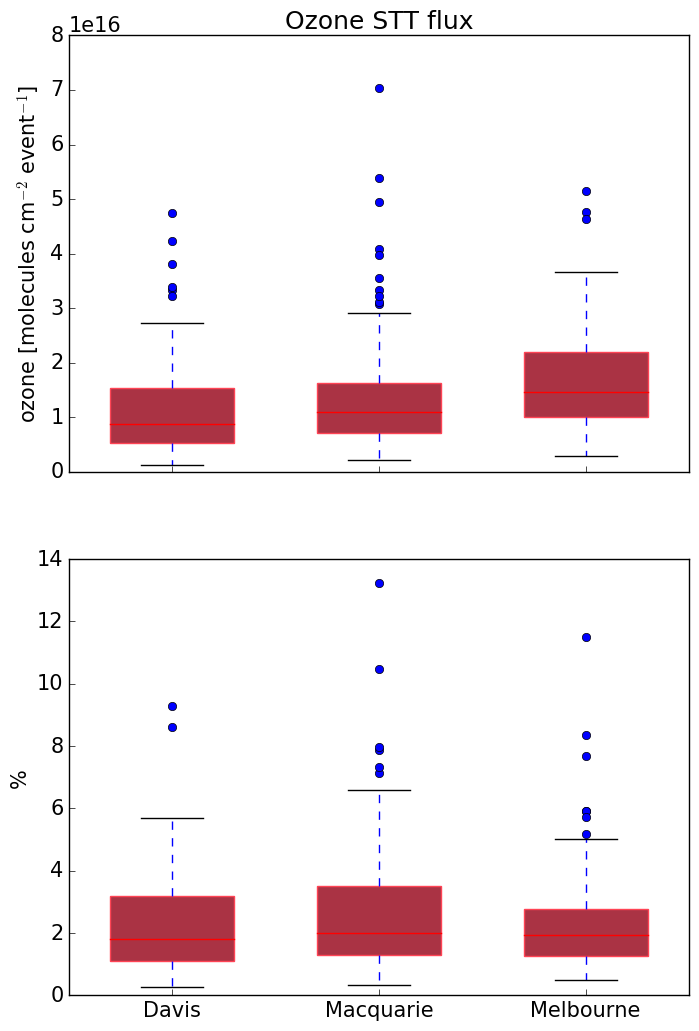
\includegraphics[width=10cm]{Figures/Ozone/flux_boxes.png}
      \caption{%
        Top panel: tropospheric ozone attributed to STT events.
        Bottom panel: percent of total tropospheric column ozone attributed to STT events.
        Boxes show the inter-quartile range (IQR), with the centre line being the median, whiskers show the minimum and maximum, circles show values which lie more than 1.5 IQR from the median.
        Values calculated from ozonesonde measurements as described in the text.}
      \label{ch_StratOzone:fig:fluxsummary}
    \end{figure}
    
    
    \begin{figure}
      % Plot from examine_stations.py in stations repo
      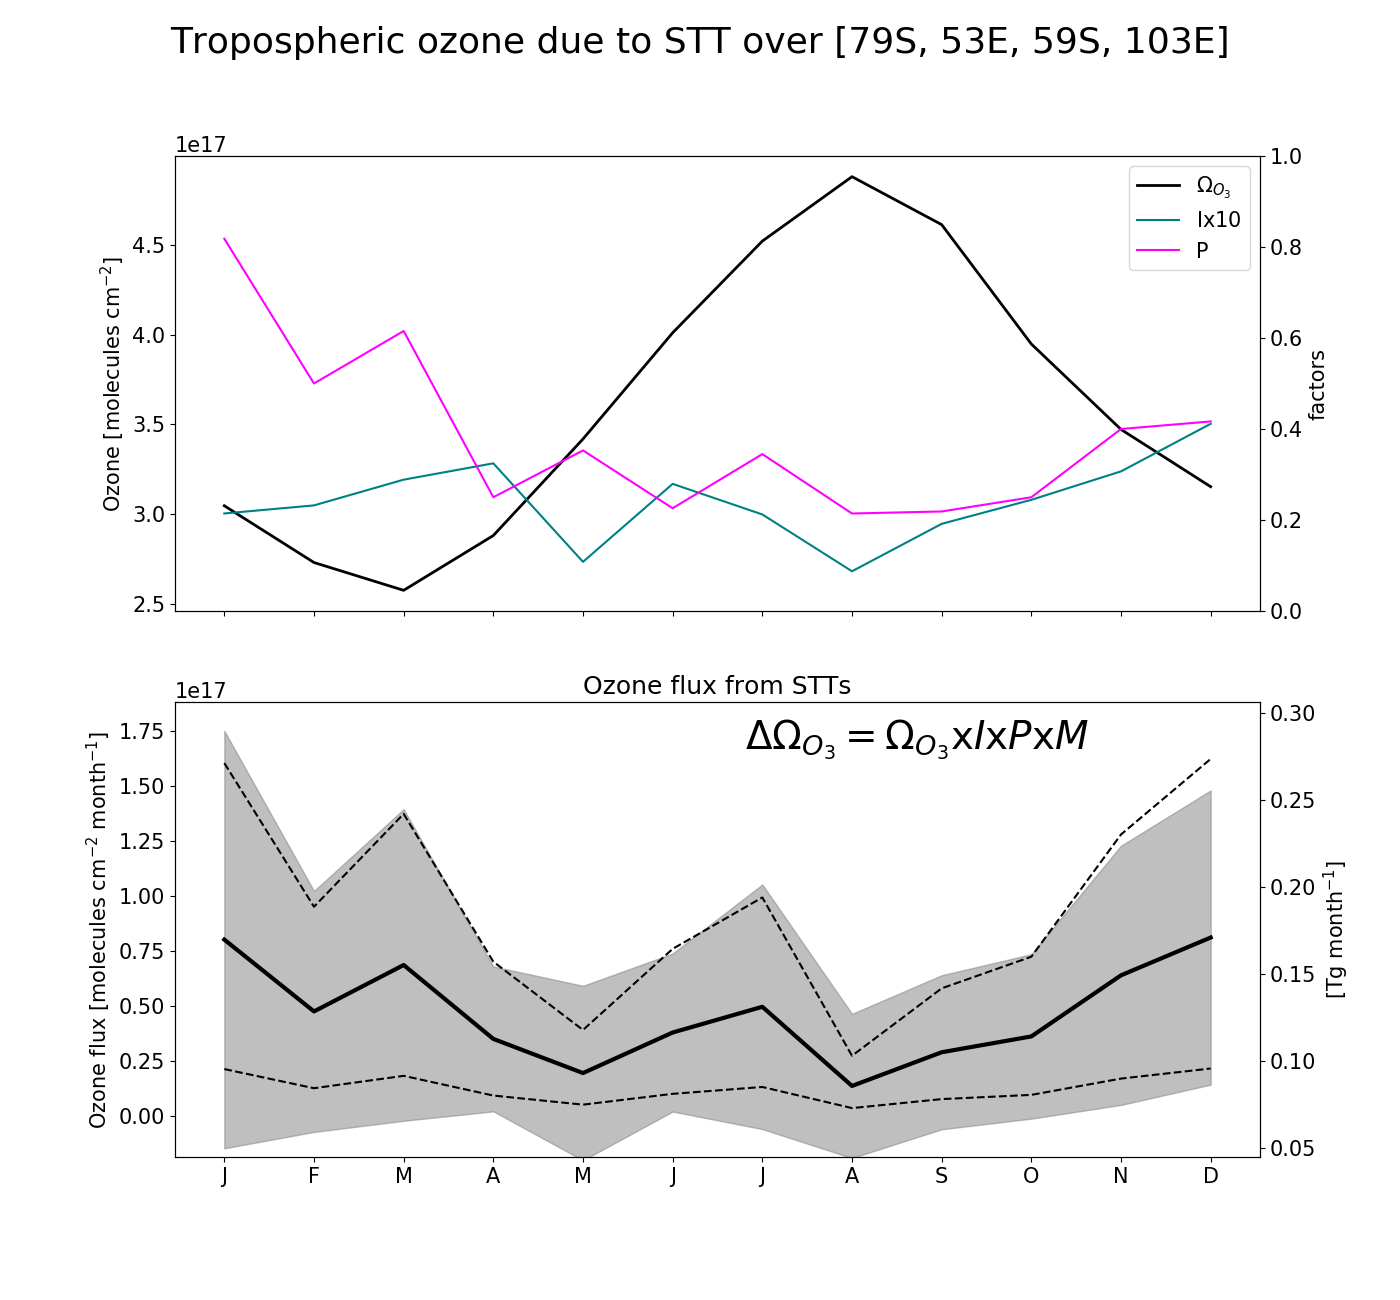
\includegraphics[width=12.0cm]{Figures/Ozone/STT_extrapolation_Dav.png}
      \caption{%
        (Top) Tropospheric ozone, ($I$)mpact per event, and ($P$)robability of event detection per sonde launch, averaged over the region above Davis.
        The tropospheric ozone column $\Omega_{O_3}$ (black, left axis) is from GEOS-Chem, while the STT probability  $P$(magenta, right axis) and impact $I$ (teal, right axis) are from the ozonesonde measurements.
        The STT impact is multiplied by ten to better show the seasonality.
        (Bottom) Estimated contribution of STT to tropospheric ozone columns over the region, with uncertainty (shaded area) estimated as outlined in Sect. \ref{ch_StratOzone:sec:sensitivity}.
        The black line shows STT ozone flux if event lifetime is assumed to be two days, with dashed lines showing the range of flux estimation if we assumed events lasted from one day to one week.}
      \label{ch_StratOzone:fig:DavExtrapolation}
    \end{figure}
    
    \begin{figure}
      % Plot from examine_stations.py in stations repo
      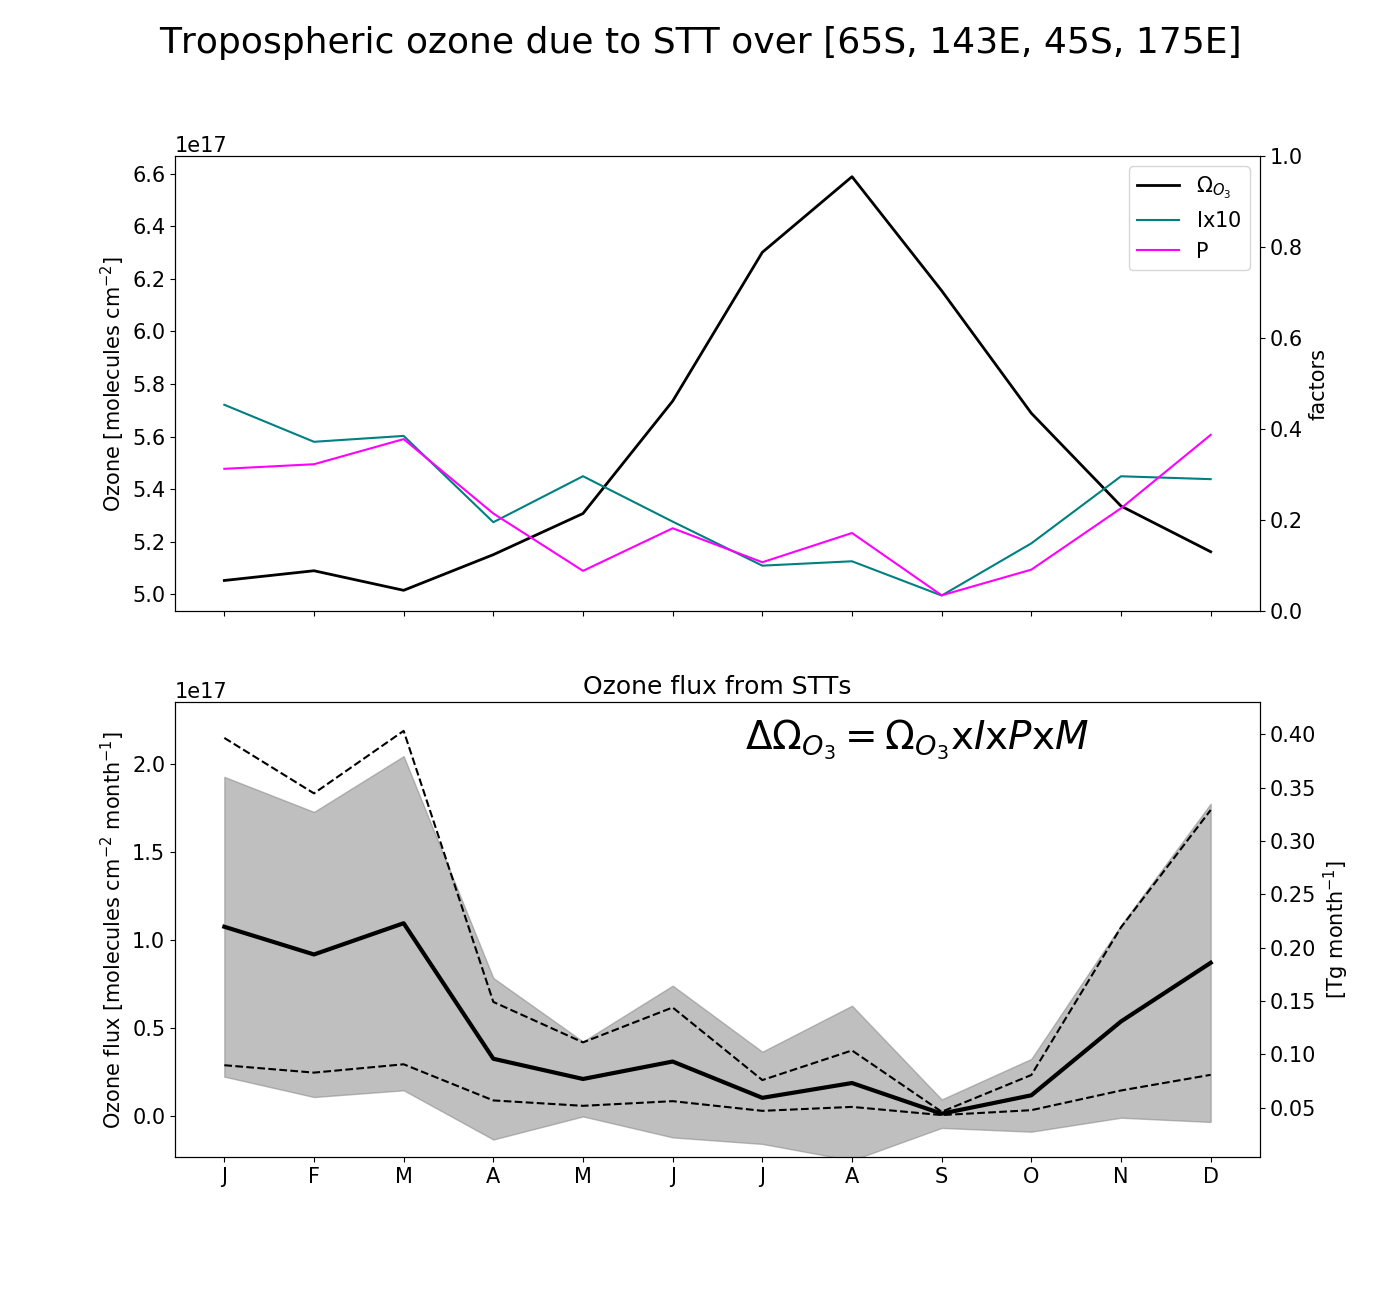
\includegraphics[width=12.0cm]{Figures/Ozone/STT_extrapolation_Mac.png}
      \caption{%
        As described in \ref{ch_StratOzone:fig:DavExtrapolation}, for the region containing Macquarie Island.}
      \label{ch_StratOzone:fig:MacExtrapolation}
    \end{figure}
    
    \begin{figure}
      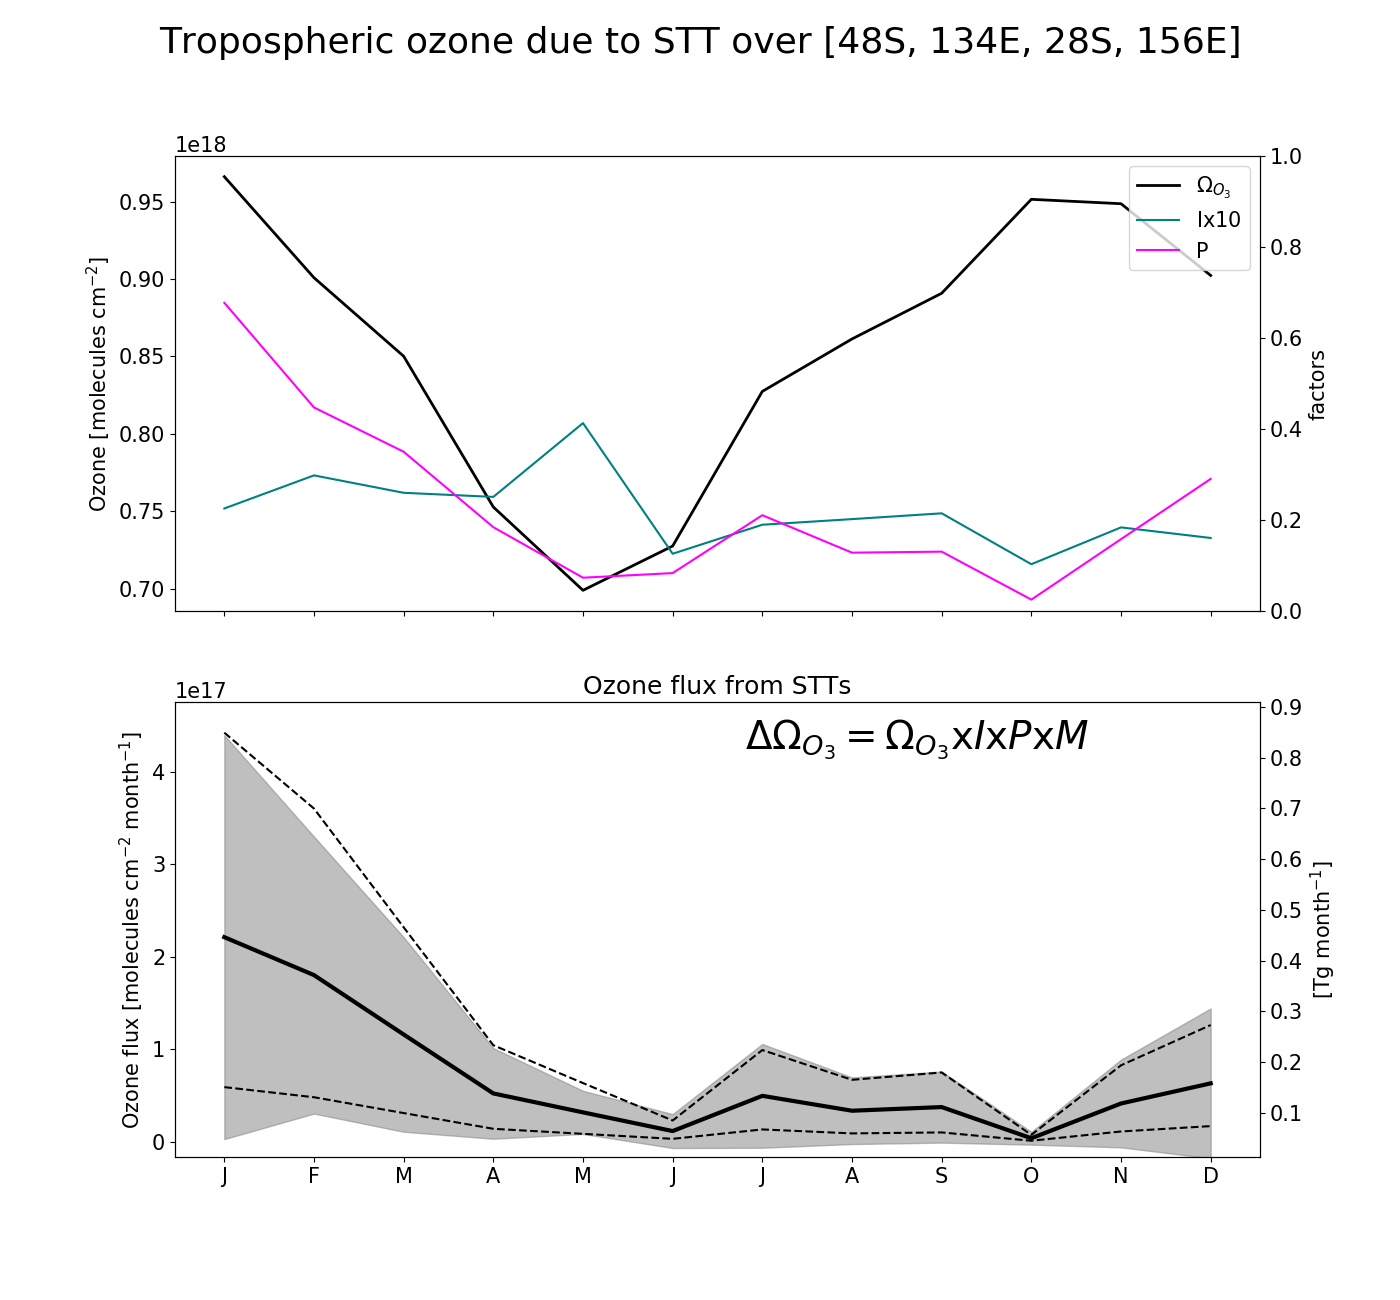
\includegraphics[width=12.0cm]{Figures/Ozone/STT_extrapolation_Melb.png}
      \caption{%
        As described in \ref{ch_StratOzone:fig:DavExtrapolation}, for the region containing Melbourne.}
      \label{ch_StratOzone:fig:MelbExtrapolation}
    \end{figure}
    
    The upper panels in figures \ref{ch_StratOzone:fig:DavExtrapolation}-\ref{ch_StratOzone:fig:MelbExtrapolation} show the factors $I$, $P$, and $\Omega_{O_3}$ which are used along with the assumed event lifetime to estimate the STT flux.
    The tropospheric ozone and area of our region is calculated using the output and surface area from GEOS-Chem over our three regions.
    The lower panel of these figures show the results of the calculation when we choose two days for our flux estimation, with dotted lines showing the range of flux calculated if we assume events last from one day to one week.
    The seasonal cycle of ozone flux is mostly driven by the $P$ term, which peaks in the SH summer over all three sites.
    Total uncertainty (shaded) is on the order of $100\%$ (see Sect. \ref{ch_StratOzone:sec:fluxuncertainty}). 
    We calculate the annual amount based on the sum of the monthly values.
    The regions over Davis, Macquarie Island, and Melbourne have estimated STT ozone contributions of $\sim 5.7 \times 10^{17}$, $\sim 5.7 \times 10^{17}$, and $\sim 8.7 \times 10^{17}$ molecules cm$^{-2}$ a$^{-1}$ respectively, or equivalently $\sim 2.0$, 2.1, and 3.3~Tg a$^{-1}$.
  
  \subsection{Comparison to literature}
    \cite{Skerlak2014} show an estimate of roughly 40 to 150~kg km$^{-2}$ month$^{-1}$ in these regions, over all seasons (see Fig. 16, 17 in their publication) while we estimate from 0 to 180~kg km$^{-2}$ month$^{-1}$ STT impact, following a seasonal cycle with the maximum in austral summer.
    We estimate higher maximum flux over Melbourne, (178, and 150~kg km$^{-2}$ month$^{-1}$ in January and February) than in either Davis (89~kg km$^{-2}$ month$^{-1}$ in March) or Macquarie Island (68~kg km$^{-2}$ month$^{-1}$ in January).
    Our calculated seasonal contributions, along with total uncertainty are shown in Table \ref{ch_StratOzone:fig:extrapolationResults}.
    
    \begin{table}[t]
      \captionsetup{justification=centering}
      \caption{Seasonal STT ozone contribution in the regions near each site, in kg km$^{-2}$ month$^{-1}$. In parentheses are the relative uncertainties.}
      \begin{tabular}{ l l l l l } 
        \hline
        Region & DJF & MAM & JJA & SON \\
        \hline
        Davis        &  54.5 (102\%) & 47.7 ( 97\%) & 30.7 (114\%) & 18.8 (127\%)\\ 
        Macquarie Island   & 61.3 ( 85\%) & 70.7 ( 91\%) & 17.9 (139\%) &  7.7 (229\%) \\
        Melbourne   & 96.7 (103\%) & 88.6 ( 89\%) & 26.7 (102\%) & 21.4 (109\%) \\
        \hline
      \end{tabular}
      \label{ch_StratOzone:fig:extrapolationResults}
    \end{table}
    
    This result disagrees with several other studies which have found STT ozone fluxes in the SH extra-tropics are largest from autumn or winter to early spring.
    \cite{Roelofs1997} used a model carrying a tracer for stratospheric ozone to estimate STT impacts. 
    They see higher SH tropospheric ozone concentrations, as well as STT flux, in the SH winter.
    Our model also shows ozone column amounts peaking in winter, however flux is maximised in summer due to our detected event frequencies.
    % Note: Roelofs model suggested equal trop o3 contribution from STT and production...
    \cite{Elbern1998} examine STT using ECMWF data for prior to 1996, using PV and Q-vectors to determine STT frequency and strength, and suggest fewer fold events in the SH occur from December to February.
    \citet{Olsen2003} used PV and winds from the GEOS reanalysis combined with ozone measurements from the TOMS satellite to estimate that the ozone flux between 30$^{\circ}$ S and 60$^{\circ}$ S is 210~Tg yr$^{-1}$, with the maximum occurring over SH winter.
    \citet{Liu2017} model the upper tropospheric ozone and its source (emissions/lightning/stratospheric) over the Atlantic ocean between 30$^{\circ}$ S and 45$^{\circ}$ S, and suggest that most of this is transported from the stratosphere from March to September, which is when the subtropical jet system is strongest.
    
    The disagreements largely reflect the difference between point source based estimates and zonally averaged estimates, as the meteorological behaviour at our three sites is not the same as the system that dominates the southern hemisphere in general.
    As detailed in Sect. \ref{ch_StratOzone:sec:eventclimatologies}, the maximum STT influx which occurs during SH winter is almost entirely due to the dominant STT system which occurs annually over the southern Indian ocean and middle of Australia.
    It is difficult to compare remote ozonesonde datasets with area averaged models or re-analyses based on non-co-located measurements (such as ERA).

\section{Sensitivities and limitations}
  \label{ch_StratOzone:sec:sensitivity}
  \subsection{Event detection}
    Our method uses several subjectively-defined quantities in the process of STT event detection.
    Here we briefly discuss these quantities and the sensitivity of the method to each.
    Using the algorithm discussed in Sect. \ref{ch_StratOzone:sec:CharacterisationOfSTTs}, we detect 80 events at Davis, 105 (21 fire influenced) events at Macquarie Island, and 127 (27 fire influenced) events at Melbourne.
    
    The cut-off threshold (defined separately for each site) is determined from the 95th percentile of the ozone perturbation profiles between 2~km above the earth's surface and 1~km below the tropopause.
    We use the 95th percentile because at this point the filter locates clear events with fewer than 5\% obvious false positive detections.
    Event detection is sensitive to this choice; for example, using the 96th, and 97th percentile instead decreased detected events by 2, 9 (2,10\%) at Davis, 13, 31 (11, 28\%) at Macquarie Island, and 8, 24 (6, 18\%) at Melbourne.
    Event detection is therefore also sensitive to the range over which the percentile is calculated.
    This range was chosen to remove anomalous edge effects of the Fourier bandpass filter and to discount the highly variable ozone concentration which occurs near the tropopause.
    
    Ozone enhancements are only considered STT events if they occur from 4~km altitude up to 500~m below the tropopause.
    This range removes possible ground pollution and events not sufficiently separated from the stratosphere, while still capturing many well-defined events that occur within 1~km of the tropopause.
    An example of a well-defined event that occurs within 1~km of the tropopause is shown in the supplementary (Fig. S2).
    However, STT events which reach below 4~km are physically possible and we may have some false negative detections due to the altitude restricted detections.
    
    %The event detection was less sensitive to the choice of Fourier bandpass scales: widening the allowed scales from the range 0.5-5.0~km to 0.4-5.1~km increased the detected events by 3 at Melbourne and 2 at Macquarie Island. 
    %Meanwhile, 2 fewer events were detected at Davis because the change to bandpass scales resulted in an increase in the threshold value calculated from the perturbed profiles (removing some detected events which were no longer larger than the new threshold).
  
  \subsection{Flux calculations}
    \label{ch_StratOzone:sec:fluxuncertainty}
    Flux is calculated as $ I \times P \times M \times \Omega_{O_3}$, with each term calculated as described in Sect. \ref{ch_StratOzone:sec:fluxcalc}.
    The uncertainty is determined using the standard deviation of the product, with variance calculated using the variance of a product formula, assuming that each of our terms is independent: 
    \begin{equation*} var(\Pi_i X_i) = \Pi_i ( var(X_i) + E(X_i)^2 ) - (\Pi_i E(X_i))^2 \end{equation*}
    The standard deviations for the $I$ and $\Omega_{O_3}$ terms are calculated over the entire dataset.
    These terms are considered to be homoskedastic (unchanging variance over time).
    Uncertainty in assumed event lifetime is set at 50\%, as we believe it is reasonable to expect events to last 1-3 days.
    $P$ is the probability of any ozonesonde detecting an event, and is assumed to be constant (for any month).
    The overall uncertainty as a percentage is shown in parentheses in Table \ref{ch_StratOzone:fig:extrapolationResults}, these values are on the order of 100\%, largely due to relative uncertainty in the $I$ factor which ranges from 50-120\% for each month.
    
    Small changes in the region don't have a large affect on the per area flux calculations: increasing or decreasing the regions by 1$^{\circ}$ on each side ($\sim 10\%$ change in area) change the resulting flux by $\sim 1\%$. % units of ~Kg cm$^{-2}$.
    However due to the large portion of winter STT events being flagged due to potential smoke plume influence, a significant change in the yearly flux is seen when we don't remove these events.
    Without removing smoke flagged events we see an increase in estimated yearly flux of $\sim 1.1, 2.1 \times 10^{17} $~molecules cm$^{-2}$ yr$^{-1}$ (which is a change of $\sim 15, 20\%$), over Macquarie Island and Melbourne respectively.
    
    Considering the $I$ factor, as discussed in here and in Sect. \ref{ch_StratOzone:sec:sensitivity}, there are several uncertainties in our method that are likely to lead to a low bias, such as the conservative estimate of flux within each event.
    Although there is little available data on SH ozone events for us to compare against, consider \citet{Terao2008}, who estimated that up to 30--40\% of the ozone at 500~hPa was transported from the stratosphere, in the northern hemisphere.
    
    Our STT event impact estimates have some sensitivity to our biomass burning filter: including smoke-influenced days increases the mean per area flux by 15-20\%.
    Although events which are detected near fire smoke plumes are removed, some portion of these could be actual STTs.
    The change in our P parameter when we include potentially smoke influenced events leads to a yearly estimated STT of 11$\times 10^{17}$ molecules cm$^{-2}$ yr$^{-1}$ over Melbourne, which suggests that up to $2.1 \times 10^{17}$ molecules cm$^{-2}$ yr$^{-1}$ ozone enhancement could be caused by smoke plume transported precursors.
    This is a potential area for improvement, as a better method of determining smoke influenced columns would improve confidence in our estimate.
    
    Other possibly important uncertainties in our calculation of STT flux which we don't cover are listed here.
    Filtering events which occur within 500~m of the tropopause may also lead to more false negatives.
    This could also cause lower impact estimates due to only measuring ozone enhancements which have descended and potentially slightly dissipated.
    On the other hand we have no measure of how often the detached ozone intrusion reascends into the stratosphere, which would lead to a reduced stratospheric impact.
    The estimated tropospheric ozone columns modelled by GEOS-Chem may be biased, for instance \cite{Hu2017} suggest that in general GEOS-Chem (with GEOS-5 met. fields) underestimates STT, with $\sim 360$~Tg a$^{-1}$ simulated globally, compared to $\sim 550$~Tg a$^{-1}$ observationally constrained.
    Transport uncertainty is very difficult to estimate with the disparate point measurements; it's possible that detected events are (at least partially) advected out of the analysis regions, which would mean we overestimate the influx into the region, and it is also possible that we are influenced by STT events outside the regions of analysis.
    Uncertainty in event longevity is set to 50\%, however this implies a very simplistic model of event lifetimes. 
    A great deal of work could be done to properly model the regional event lifetimes, however this is beyond the scope of our work.
    
    Uncertainties in STT ozone flux detection are ($\sim 100\%$), and could be directly improved with larger or longer datasets.
    Possible parameterisations and an improved model of event lifetime could also improve the confidence in our estimate of event impacts, as well as allowing fewer assumptions.
    %The simple assumptions made in order to achieve an estimate of ozone flux are not feasible over larger areas, however as a preliminary or constraining estimate for a region with few measurements we believe they add to the discussion.

\section{Conclusions}

  Stratosphere-to-troposphere transport (STT) can be a major source of ozone to the remote free troposphere, but the occurrence and influence of STT events remains poorly quantified in the southern extra-tropics.
  Ozonesonde observations in the SH provide a satellite-independent quantification of the frequency of STT events, as well as an estimate of their impact and source.
  %The frequency and amount of ozone descending from the stratosphere into the troposphere can be estimated from the long time series of tropospheric ozone profiles.
  Using almost ten years of ozonesonde profiles over the southern high latitudes, we have quantified the frequency, seasonality, and altitude distributions of STT events in the SH extra-tropics. 
  By combining this information with ozone column estimates from a global chemical transport model, we provided a first, conservative estimate of the influence of STT events on tropospheric ozone over the Southern Ocean.
  
  Our method involved applying a bandpass filter to the measured ozone profiles to determine STT event occurrence and strength.
  The filter removed seasonal influences and allowed clear detection of ozone-enhanced tongues of air in the troposphere.
  By setting empirically-derived thresholds, this method clearly distinguished tropospheric ozone enhancements that are separated from the stratosphere.
  Our method is sensitive to various parameters involved in the calculation; however, for our sites we saw few false positive detections of STT events.
  
  Detected STT events at three sites spanning the SH extra-tropics (38$^{\circ}$S, 55$^{\circ}$S, and 69$^{\circ}$S) showed a distinct seasonal cycle.
  All three sites displayed a summer (DJF) maximum and an autumn to winter (AMJJA) minimum, although the seasonal amplitude was less apparent at the Antarctic site (Davis) as events were also detected regularly in winter and spring (likely due to polar jet stream-caused turbulence).
  Analysis of ERA-Interim reanalysis data suggested the majority of events were caused by turbulent weather in the upper troposphere due to low pressure fronts, followed by cut-off low pressure systems.
  Comparison of ozonesonde-measured ozone profiles against those simulated by the GEOS-Chem global chemical transport model showed the model is able to reproduce seasonal features but does not have sufficient vertical resolution to distinguish STT events.
  %The seasonal features in the ozonesonde record of tropospheric ozone columns are well represented by the model.
  %Simulated profiles generally can not identify STT events due to their lower vertical resolution.
  
  By combining the simulated tropospheric column ozone from GEOS-Chem with ozonesonde-derived STT estimates, we provide a first estimate of the total contribution of STT events to tropospheric ozone in these southern extra-tropical regions.
  We estimate that the ozone enhancement due to STT events near our three sites ranges from 300-570~kg km$^{-2}$ a$^{-1}$, with seasonal maximum in SH summer.
  
  Estimating STT flux using ozonesonde data alone remains challenging; however, the very high vertical resolution provided by ozonesondes suggests  they are capable of detecting STT events that models, re-analyses, and satellites may not. 
  Further work is needed to more accurately translate these ozonesonde measurements into STT ozone fluxes, particularly in the SH where data are sparse and STT is likely to be a major contributor to upper tropospheric ozone in some regions.
  More frequent ozonesonde releases at SH sites could facilitate development of better STT flux estimates for this region.
  %As the climate alters, an understanding of mixing between the stratosphere and troposphere over the southern ocean will help diagnose potential hazards.
  %Seasonality and impact of stratospheric ozone are changing over time, furter analysis of this long term set of ozonesonde data will be useful into the future.

%\authorcontribution{...}
\section{Contributions and Acknowledgements}
  JWG wrote the algorithms, ran the GEOS-Chem simulations, performed the analysis and led the writing of the paper under the supervision and guidance of SPA, RS, and JAF. 
  AK contributed the Davis ozonesonde data and performed the analysis of the alternate STT proxy. 
  All authors contributed to editing and revising the manuscript.

  %\competinginterests{The authors declare that they have no conflict of interest.}
  
  %\disclaimer{disclaimer}
  
  % Data availability
  %
  \textit{Data availability.} All GEOS-Chem model output and the ozonesonde observational data are available from the authors upon request.

  %\begin{acknowledgements}
  We thank Dr. Sandy Burden for help clarifying some of the uncertainties involved in methods within this work.
  We also thank Dr. Clare Paton-Walsh, who identified the need to account for smoke-influenced events, and provided discussions on how to go about doing such.
  Ozonesonde data comes from the World Ozone and Ultraviolet Data Centre (WOUDC).
  The ERA-Interim data were downloaded from the ECMWF website following registration.
  This research was undertaken with the assistance of resources provided at the NCI National Facility systems at the Australian National University through the National Computational Merit Allocation Scheme supported by the Australian Government.
  This work was supported through funding by the Australian Government's Australian Antarctic science grant program (FoRCES 4012), the Australian Research Council's Centre of Excellence for Climate System Science (CE110001028), the Commonwealth Department of the Environment ozone summer scholar program.
  This research is supported by an Australian Government Research Training Program (RTP) Scholarship.
  %\end{acknowledgements} % Ozone from the stratosphere (roughly = paper in ACP)
    
%
% ---- Chapter layout ----
%
% 1) Introduction - 
% 2) 
% ------------------------



\chapter{Biogenic Isoprene emissions in Australia} % Chapter title
\label{BioIsop}
  
%----------------------------------------------------------------------------------------
% Section 1 -- INTRO 
%----------------------------------------------------------------------------------------
\section{Introduction}  
\label{BioIsop:intro}  
  
  % What we aim to do
  We estimate isoprene emissions in Australia using top-down estimates based on recalculated OMI HCHO measurements and modelled isoprene to HCHO yields.
  These estimates are compared to several campaigns (SPS1, SPS2, MUMBA, Daintree) and used as the new boundary conditions for GEOS-Chem.
  Sensitivity to soil moisture, (maybe) LAI, and satellite AMF calculation is examined and quantified for some scenarios.
  The effect of using these new top down isoprene emissions as the boundary conditions for GEOS-Chem is studied
  Wellness of fit between in-situ (at Wollongong) HCHO, satellite (OMI), and modelled (GEOS-Chem) HCHO is determined with and without updated emissions estimates.
  
  One of the most popular emissions inventories for biogenic isoprene, the Model of Emissions of Gases and Aerosols from Nature (MEGAN).
  Global atmospheric studies often use MEGAN along with a chemical transport model (CTM) to examine transport, deposition, and various chemical processes in the atmosphere.
  Emissions of Biogenic Volatile Organic Compounds (BVOCs) including isoprene are often the subject of studies as they are still relatively uncertain, as well as being drivers for imprtant oxidation and pollution events.
  
  (MEGAN) is poorly calibrated for Australian conditions, their emissions of isoprene (C$_5$H$_8$) may be overestimated, especially in the southeast.
  \cite{Muller2008} compared MEGAN against emissions calculated using top down estimates from the GOME2 satellite measurements of formaldehyde.
  \cite{Stavrakou2015} showed that this overestimate may be a factor of 2-3 in January.
  \cite{Sindelarova2014} show how 50\% of the isoprene emissions could be reduced by accounting for lower soil moisture.
  \cite{Emmerson2016} discuss the suitability of MEGAN's isoprene and monoterpene emission factors over southeast Australia, and suggest isoprene emissions are estimated 2-6 times too high.
  They also show that no blanket increase or decrease in emission factors is appropriate for the entire southeast of Australia.
  
  % Brief isoprene to hcho description
  In the remote troposphere HCHO production is dominated by methane oxidation, while in the continental boundary layer (CBL) production is largely due to NMVOCs (\cite{Abbot2003, Kefauver2014}).
  This suggests that HCHO enhancement over continents can be used to determine NMVOC emissions.
  In the CBL, HCHO enhancement is generally driven by short lived ($<1$~hr) precursors (most importantly isoprene).
  HCHO itself has a lifetime of a few hours (\cite{Kefauver2014}).
  Isoprene is emitted and enters the atmosphere in the gas phase, where it begins a complex series of reactions.
  Formaldehyde is produced with high yields in many of the isoprene reactions, which are discussed in more detail in Section \ref{LR:VOCs:IsopCascade}.
  HCHO measurements are often used as a check on how well isoprene reactions are simulated, as model output can then be compared against them \citep{Marvin2017}.
  
  
  
  % TODO: monoterpenes outline, here or elsewhere?
  Isoprene and monoterpene emissions are both very uncertain in Australia.
  Monoterpene oxidation by O$_3$, OH and NO$_3$ radicals may also form aerosols, with the reaction with ozone forming the most particles \citep{Kanakidou2005}.
  
  \subsection{Top-down emissions estimates}
    There are now a few methods of estimating isoprene emissions using satellite measurements of emission products, here I describe them and briefly compare the pros and cons of each.
    
    \subsubsection{Linear}
      \label{BioIsop:intro:top_down_linear}
      
      %TODO: Paul palmer outline of technique for top-down estimate
      This technique is the simplest, and is performed in this thesis.
      With the vertical columns of biogenic HCHO we can infer the local (grid space) isoprene emissions using effective molar formaldehyde yield (In other continents around 2-3, or 1 in low NO$_X$ conditions) \citep{Palmer2003,Marais2012,Bauwens2016}.
      If we assume there is fast HCHO yield, so that the effect of chemical transport is minimal, and that HCHO and isoprene are at steady states, then we can calculate local yield from our CTM.
      %This yield is derived from both HCHO and isoprene, such as was used by \citet{Millet2006} who produced a molar HCHO yield of 2.3 in north eastern USA.
      Yield is calculated from the modelled slope between isoprene emissions and HCHO total column within each gridbox over Australia, as performed in \cite{Palmer2003}, using modelled values between 1200-1400 LT which is around the overpass time of the OMI.
      This modelled yield is then used in conjunction with the recalculated OMI measurements in order to estimate isoprene emissions.
      To calculate emissions we use a reduced major axis (RMA) regression between modelled average values of the loss rates and total columns, an example is shown in figure TODO: figure with RMA of these over whatever time and space I end up using.
      
      % TODO: Pros and cons of PP top down method
      % Pros and cons:
    
    \subsubsection{Bayesian}
      Satellite based emissions estimates may allow us to improve the models without requiring lots of hard work on calibrating MEGAN to the large data sparse continent of Australia.
      Emissions of monoterpenes (C$_10$H$_16$, two units of isoprene) may also be underestimated in southeastern Australia, which could lead to the unique scenario of neither type of emission dominating VOC chemistry over the forests \citep{Emmerson2016}.
      
      % Top down emissions estimation methods:
      Another method of correcting isoprene emissions using observed HCHO total column involves a Bayesian inversion.
      \cite{Shim2005} work with GOME HCHO observations and GEOS-Chem, looking at areas with high signal to noise ratio (higher HCHO concentrations).
      They show that the model underestimates isoprene emissions and HCHO concentrations by 14-46\%, with the corrected VOC emissions reducing the model biases to 3-25\%.
      
      The Bayesian inversion is also used in \cite{Curci2010}, where a regional CTM (CHIMERE) simulates HCHO, which is compared against OMI observed HCHO and shown to be regionally biased.
      This bias is expected to be caused by errors in MEGANs isoprene emissions estimations.
      The CHIMERE model is used to derive yields of HCHO from the various local VOCs and these are then used in estimating local emissions.
      The model is run initially with emissions of BVOCs and reactive anthropogenic VOCs (RAVOCs) turned off in order to work out the background (b) values of these compounds.
      The Bayesian inversion is used to correct regionally biased biogenic isoprene emissions by optimising these parameters in order to simulate HCHO closest to the observed HCHO levels.
      \cite{Curci2010} uses CHIMERE as the forward model to determine the relationship between HCHO (y), isorene and reactive anthropogenic VOCs (\textbf{x}), using 
      \begin{equation}
      y=\mathbf{K}x + b + \epsilon
      \end{equation}
      where $\epsilon$ are the (assumed) independent errors in measurements.
      K is the Jacobian matrix determined from CHIMERE representing the sensitivity of y to the state variable x.
      This K matrix is used in conjunction with error covariance in x to determine the Maximum A Posteriori (MAP) solution to calculate the optimal estimate of x ($\hat{x}$).
  
  
  \subsection{Aims}
    
    %% AIMs paragraph
    Here we introduce how uncertain isoprene emissions are over Australia, and discuss literature which shows how the estimates may be too high.
    Section \ref{BioIsop:Data} describes the model, satellite, and campaign data we use to determine and analyse isoprene emissions.
    The OMI measurements used in this research are recalculated using an updated estimate of HCHO profiles and validated against Wollongong total column measurements.
    Section \ref{BioIsop:Methods} lays out how the isoprene emissions are estimated, and the results are examined in Section \ref{BioIsop:Results}
    
  
  
\section{Methods}
  \label{BioIsop:Methods}
  
  % Method Briefly outlined here
  Here is an overview of the steps involved in my Thesis, which take satellite data and model output to estimate isoprene emissions.
  \begin{enumerate}
    \item Download Aqua/Terra MODIS gridded fire counts (MOD14A1), smoke measurements (OMAERUVd), and Aura HCHO columns (OMHCHO).
    \item Run GEOS-Chem with satellite overpass output averaged over 1200-1300~LT (matching Aura overpass time)
    \item Recalculate OMHCHO vertical columns using GEOS-Chem to recreate the shape factors for each slant column. Also done with code from Paul Palmers group which includes recalculation of the scattering weights.
    \item 
      Mask HCHO columns which occur on days with non-zero (MODIS) fire counts over the prior 8 days, as is done in \cite{Marais2012}.
      More detail on this step can be found in \ref{Model:Filter:fire}
    \item TODO: Filter gridsquares where OMI AAOD (OMAERUVd) is over some threshhold to be determined (ALSO TODO)
    \item TODO: Filter NOx influenced grid squares.
    \item Biogenic Yield calculated in each 2x2.5\degr grid square using daily averaged HCHO from biogenic only run of GEOS-Chem, linearly corellated with MEGAN isoprene emissions within those squares
    \item TODO: Biogenic yield masked when smearing term is above a threshhold (TODO: determine)
    \item Yield (actually regression slope between hcho and emissions) multiplied against recalculated OMI HCHO to provide top down isop emissions estimate
    \item compare against MEGAN, MUMBA, SPS, Daintree, Wollongong, and one set of airplane(?) measurements
  \end{enumerate}
  
  %TODO Full method outline to Jenny
  \subsection{}
  
  \subsection{Satellite inversion}
  \label{BioIsop:SatInv}
  
    % Lead in to satellite inversion
    Top-down estimates look at how much of a chemical is in the atmosphere and try to work out how much of its major precursors were emitted.
    This generally takes advantage of longer lived products which may reach a measurable equilibrium in the atmosphere.
    For isoprene this is done by looking at atmospheric HCHO enhancement, which can be largely attributed to isoprene emissions once transport and other factors are accounted for.
    Recently \cite{Stavrakou2015} used satellite HCHO measurements to constrain anthropogenic sources of isoprene and found good global agreement with the bottom up estimates, although some regions had sources differ by up to 25-40\%. 
    Their study used the RETRO 2000 database for anthropogenic emission aprioris except for Asia in 2008 where REASv2 was used. 
    Since 1997, when GOME first measured HCHO over Asia \citep{Thomas1998}, satellites have been able to provide a total column measurement of HCHO, one of the primary products of isoprene.
    
    Satellites recording reflected solar spectra use DOAS to measure various trace gases in the atmosphere, including formaldehyde. 
    While satellite measurements can only be used during daytime hours, HCHO lifetimes are sufficiently short that any night-time chemistry will not affect midday observations \citep{Wolfe2016}.
    Satellites can be used to measure the seasonal and interannual variability of HCHO over the globe.
    These records can be compared with modeled estimates of HCHO and used as a proxy to estimate isoprene emissions.
    This has been done in North America \citep{Palmer2003, Millet2006}, South America, Africa, China, Europe \citep{Dufour2009}, and recently globally \citep{FortemsCheiney2012, Bauwens2016}.
    Often these works use two forms of measurement such as satellite and aircraft data combined for validation (\cite{Marais2014}).
    There is less information available from satellite measurements at higher latitudes due to increased errors (\cite{DeSmedt2015}).
    
    Using HCHO to determine emissions of isoprene was initially performed by \cite{Palmer2001, Palmer2003}, who used in-situ summertime HCHO measurements over North America as model validation.
    Isoprene emissions fluxes were derived using the Global Ozone Monitoring Experiment (GOME) satellite instrument.
    Palmer's method improved biogenic isoprene emissions estimates (compared with in-situ measurements) over two available inventories: the U.S. EPA Biogenic Emissions Inventory System (BEIS2) and the Global Emissions Inventory Activity (GEIA).
    This showed an inversion technique which could be used to improve large scale emissions estimates without further expensive measurement campaigns.
    
    %TODO
    TODO: Read through this list of sources on the hcho to isop process : taken from Wolfe2015
    Such techniques have informed isoprene emission inventories in North America (Abbot et al., 2003; Millet et al., 2008 (\cite{Palmer2003,Millet2006,Palmer2006})), South America ((\cite{Barkley2013}), 2008), Europe (\cite{Curci2010,Dufour2009}), Africa (\cite{Marais2012}), Asia (Fu et al., 2007; Stavrakou et al., 2014), and globally (Fortems-Cheiney et al., 2012; (\cite{Shim2005}); Stavrakou et al., 2009).
    
    Initially studies assumed a simple linear steady-state relationship between HCHO and it's precursors (\cite{Palmer2003, Palmer2006, Millet2006}).
    This allowed a simple calculation of isoprene using the measured HCHO, with estimated reaction rates and yields.
    The methodology for calculating VOCs from HCHO is laid out in \cite{Palmer2003}, and takes into account the expected lifetime and reaction rates of the precursor VOCs and HCHO.
    Assuming HCHO is produced quickly from short-lived intermediates, and the column is at steady state:
    \begin{eqnarray*}
      VOC_i \overset{k_i}{\rightarrow} Y_i HCHO
    \end{eqnarray*}
    Where $Y_i$ is HCHO yield per C atom (a measure of how much HCHO will form per gram of C from a VOC within a system), and $k_i$ is the reaction rate.
    Then assuming a steady state of atmospheric HCHO ($\Omega$ molecules $cm^{-2}$) produced by oxidation of VOCs (VOC$_i$) and no horizontal transport:
    \begin{eqnarray*}
      \Omega = \frac{1}{k_{HCHO}} \sum_{i} Y_i E_i
    \end{eqnarray*}
    Where i indexes a chemical species, $k_{HCHO}$ is the HCHO loss rate due to OH and photolysis, Y$_i$ is the molar HCHO yield from oxidation of i, and $E_i$ is emission fluxes ( C atoms $cm^{-2}s^{-1}$).
    
    Estimates of Y$_i$ can be attained from a model as shown in \cite{Millet2006}.
    This involves a reduced major axis (RMA) correlation calculation between modelled HCHO and isoprene columns, multiplied by their loss rates (to photolysis and oxidation) (as a normalising factor).  
    In high NOx environments where HCHO has a lifetime on the order of 30 minutes, it can be used to map isoprene emissions with spatial resolution from 10-100 kms.
    Horizontal transport 'smears' the HCHO signal so that source location would need to be calculated using windspeeds and loss rates (\cite{Palmer2001,Palmer2003}).
    Smearing is explicitly handled in these studies due to the importance of transport and NO$_X$ on forming robust and accurate estimates.
    Over Australia NO$_X$ levels are generally not high enough to ensure quick HCHO formation and we must take extra care that we can account for the transport or 'smearing' caused by slower HCHO formation, details on this process can be found in Section \ref{BioIsop:Methods:Smearing}.
    
    
    
    
    More recently, full inversions that better account for transport, source attribution, and chemical schemes have been implemented (\cite{FortemsCheiney2012}).
    TODO: full description of this better inversion technique going through FortemsCheiney2012.
    
    \cite{Kefauver2014} reviews remote sensing of BVOCs, which are on the rise, examining the last 20 years of data and analysis of the satellite products.
    Their review encompasses the latest reports up to 2014.
    The modelled isoprene and BVOC emissions from MEGAN \citep{Guenther2000} of 500 and 1150~Tga$^{-1}$ respectively are still the global go to estimates.
    Their review reinforces the message that NMVOCs affect the oxidative capacity of the atmosphere and are largely driven by and sensitive to vegetation.
    The tropospheric affects from NMVOCs on the hydroxyl radical (OH), ozone (O$_3$), SOAs, and methane longevity, all interconnect to form a very complex system which still suffers from relatively large uncertainties in both measurement and chemistry mechanisms.
    One focus of \cite{Kefauver2014} is HCHO, which is the dominant product of most BVOCs which is measurable by remote sensing.
    The main datasets of HCHO are from four satellite instruments: GOME on ERS-2, SCIAMACHY on ENVI-SAT, OMI on EOS AURA, and GOME2 on MetOp-A.
    These satellites have slightly different spectral and spatial resolutions, as well as using varied processes to estimate HCHO from detected radiances.
    This can lead to different estimates between instruments or methodologies as described in \cite{Lorent2017}, which means validation and comparison is more important when using these remotely sensed data.
    
    Total HCHO is measured by satellite over the entire world, however the technique is not perfect and suffers from uncertainties and interferences.
    Satellite based chemical concentrations rely on ground-based measurements and modelled data for validation.
    They provide various readings with daily global coverage which is not otherwise feasable.
    
    Validation is important due to the various uncertainties in the satellite remote sensing process, with apriori assumptions having the greatest effect on structural uncertainty between measurements techniques \cite{Lorente2017}.
    \cite{Zhu2016} use SEAC$^4$RS aircraft HCHO measurements over the southeastern US as model validation, and show a bias in the assumed OMI shape factor that leads to a bias between satellite and SEAC$^4$RS measurements.
    \cite{Marais2014} compare OMI based isoprene emission estimates against relaxed eddy accumulation measurements from African field campaigns, as well as MEGAN and GEOS-5 inventories.
    \cite{Dufour2009} use HCHO from SCIAMACHY, and examine Europe using CHIMERE as the chemical model. 
    In their work they show that satellite measurements can reduce source emission uncertainty by a factor of two, where emissions are relatively large.
    
  \subsection{Calculation of Emissions}
    \label{BioIsop:Calculation}
   
    % FIRST: outline of what we do
    As is done in \citet{Palmer2003, Millet2006, Bauwens2016}, we assume that HCHO, and Isoprene columns are in a steady state, with no horizontal transport.
    We also assume that isoprene is the only compound enhancing the HCHO levels, which requires that we filter out influence from fires.
    Emissions of precursors are easy to calculate as long as we know the molar HCHO yields (Y$_i$) and effective chemical loss rates (k$_i$):
    \begin{equation}
    \Omega_{HCHO} = \frac{1}{k_{HCHO}}\Sigma_i k_i Y_i \Omega_i = \frac{1}{k_{HCHO}}\Sigma_i Y_i E_i
    \end{equation}
    This works if there is fast HCHO yield, so that the effect of chemical transport is minimal.
    The background HCHO is calculated using measurements in the remote pacific at the same time and latitude.
    Table \ref{BioIsop:Methods:tab_VOCAusYields} shows the average yield calculated for Australia. (TODO: this table and some notes)
    
    %% SLOPE Calculation
    In order to approximate the isoprene to HCHO yields over Australia, GEOS-Chem is run and the slope (S) between modelled tropospheric HCHO columns and emissions of isoprene within each grid box. 
    Figure (TODO: example grid box and regression plot.) shows the regression between emitted isoprene and tropospheric column HCHO, averaged between 1200-1300~LT each day.
    We can infer the local (grid space) isoprene emissions (E$_{isop}$) using effective formaldehyde yield from isoprene ($Y_{isop}$).
    \begin{equation} \label{BioIsop:Calculation:eqn_isop_yield}
    \Omega_{HCHO} = S \times E_{isop} + B
    \end{equation}
    Where \textit{B} is the background HCHO, and $S = Y_{isop}/k_{HCHO}$ is determined monthly as the regression between $\Omega_{HCHO}$ and E$_{isop}$ on daily saved outputs from GEOS-Chem over Australia using 2 by 2.5$^{\circ}$ horizontal resolution. 
    Modeled background emissions can be ignored here as they do not affect the slope calculation.
    Once we have calculated this slope, we use the same formula (Eqn. \ref{BioIsop:Calculation:eqn_isop_yield}) to determine the isoprene emissions.
    By replacing $\Omega_{HCHO}$ and $B$ with OMI based values, $E_{isop}$ is the only unknown.
    
    %% NOTE: Satellite uncertainty bounds for slope calculation
    In several studies OMI satellite HCHO columns are scaled up by up to 40\% to match in-situ measurements TODO:citations.
    Since we don't have enough in-situ data to reasonably scale the satellite columns we instead re-run the calculation with them scaled up by 40\% and consider this as a possible bound on satellite uncertainty.
    Yield and estimated top-down emissions are therefore given an upper and lower bound on satellite based uncertainty through this method.
    
    %% BACKGROUND calculation(s)
    There are a couple of ways to determine the modelled background HCHO concentration, one of which involves running the model with isoprene emissions turned off, which allows us to see exactly how much the modelled isoprene emissions alter each vertical column of HCHO.
    This is effective since we have assumed variation in HCHO columns only depends on isoprene emissions, so our background term is theoretically identical to the emission free simulated HCHO.
    The other way involves looking at HCHO over the remote pacific at matching latitudes and times, which emulates how the background is determined for the measured HCHO.
    These modelled background HCHO concentrations are mostly used for comparison with other datasets.
    TODO: show how these two numbers compare! figure with time series of both backgrounds for Aus, SEAus, and remote ocean.
    
    The $B$ackground from OMI  is determined using the mean column HCHO measured over the remote pacific ocean (180-120$^{\circ}$W).
    TODO: Update the background term to do as follows: For this term we average each month of remote ocean measurements, as well as averaging longitudinally within 180-120$^{\circ}$W, and finally $B$ is estimated at each latitude using $\pm 10^{\circ}$.
    This is gives us a background which is appropriate for any latitude, and is shown in Figure TODO: figure with background region highlighted and a time series of background values.
    When calculating the $E_{isop}$ from our modeled slope with OMI HCHO and background, we end up with negative emissions wherever the OMI HCHO column is less than the OMI background (as $E_{isop} = \frac{\Omega_{HCHO} - B}{S}$).
    These are set to zero, which increases the average by around TODO: X\%.
    The measured background HCHO is the average concentration measured in the remote pacific at the same time.
    
    Figure \ref{BioIsop:Calculation:fig_E_isop_vs_hcho_model_sample} shows the modelled isoprene emissions and column HCHO concentrations along with the RMA regression line, sampled from grid boxes over Australia for January 2005.
    Some affects from the low emissions in grid boxes which are largely oceanic can be seen and are handled by TODO: handle these and document here.
    Due to the low horizontal resolution of GEOS-Chem (2 by 2.5$^{\circ}$, latitude by longitude), calculations from grid boxes on the coast which are largely oceanic need to be discarded as the change in HCHO is not dominated by emissions of isoprene, as is assumed for Eqn \ref{BioIsop:Calculation:eqn_isop_yield}.
    A nested version of GEOS-Chem allows a much better analysis of coastal regions, at 0.25 by 0.3125$^{\circ}$ resolution.
    \begin{figure}[!htbp]
      % Figure from GC_tests.py -> isop_hcho_RMA
      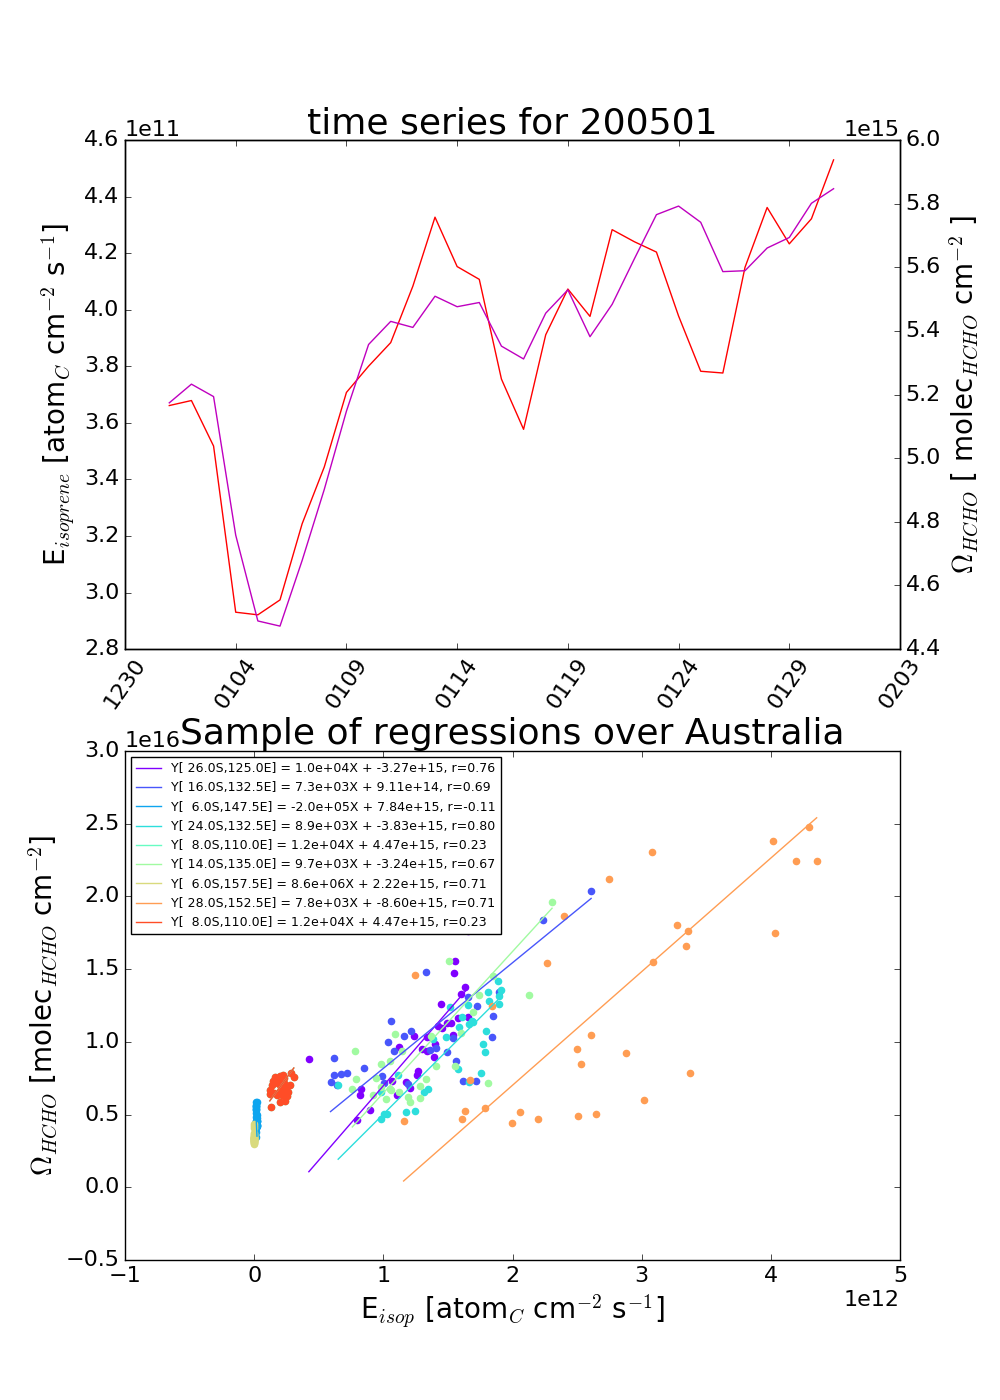
\includegraphics[width=\textwidth]{Figures/Isoprene/E_isop_vs_hcho_series_200501.png}
      \caption{%
        Top panel: isoprene emissions for January, 2005, shown in red, coplotted with tropospheric hcho columns, shown in magenta.
        Both series are daily averages over Australia.
        Bottom panel: (RMA) linear regressions from between emissions of isoprene and tropospheric hcho columns, sampled randomly from the 2$^{\circ}$ by 2.5$^{\circ}$ latitude longitude gridboxes over Australia for the month of January (2005).
      }
      \label{BioIsop:Calculation:fig_E_isop_vs_hcho_model_sample}
    \end{figure}
    
    %TODO: put this into results
    Using this modelled slope at 2$^{\circ}$ by 2.5$^{\circ}$ and applying it to equation \ref{BioIsop:Calculation:eqn_isop_yield} with B and $\Omega_{HCHO}$ calculated using OMI satellite measurements provides a new estimate of isoprene emissions.
    Figure \ref{BioIsop:Calculation:fig_E_isop_200501} shows the emissions calculated this way along with the Emissions output by GEOS-Chem averaged over January, 2005.
    \begin{figure}[!htbp]
      % Figure from Inversion.py -> check_against_MEGAN()
      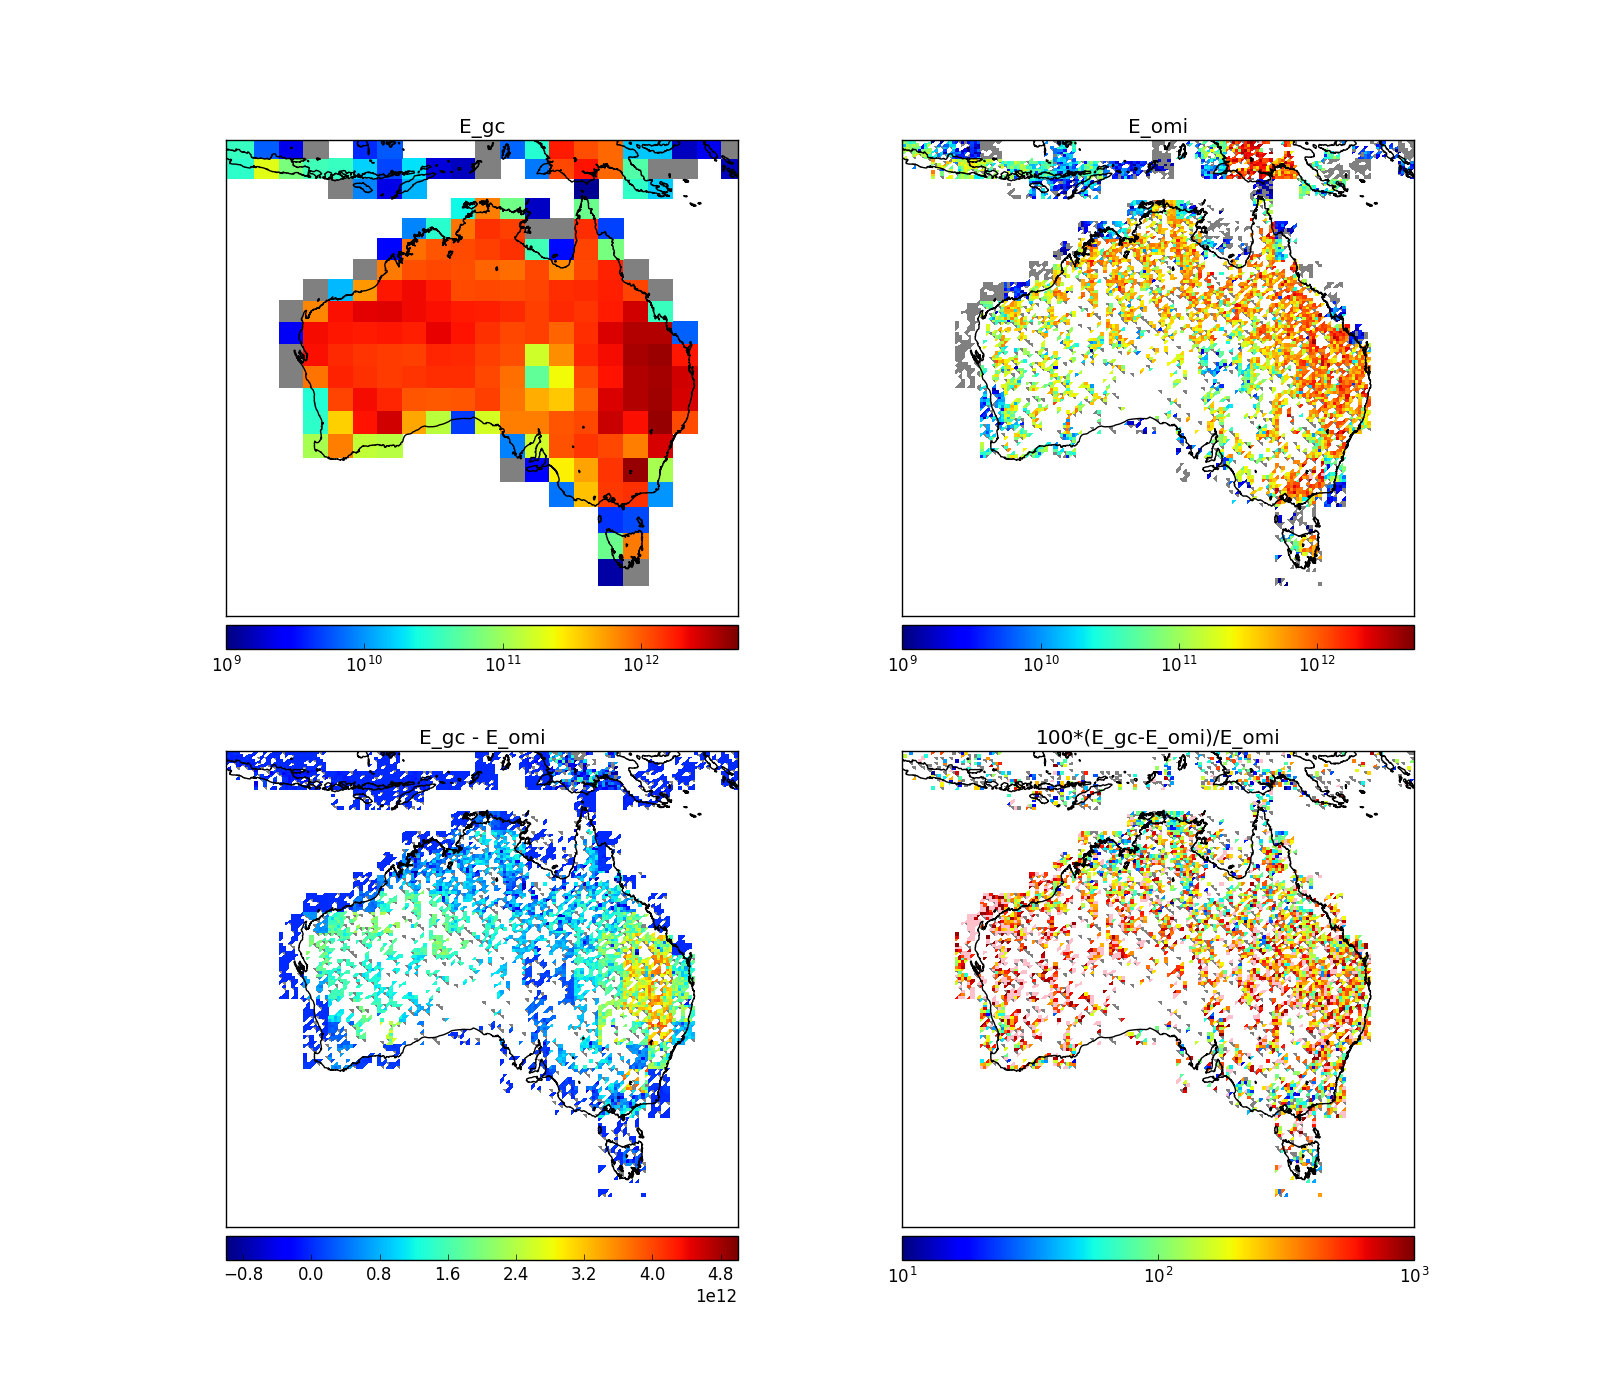
\includegraphics[width=\textwidth]{Figures/Isoprene/E_Comparison.png}
      \caption{%
        Top row is isoprene emissions for the month of January, in 2005, from GEOS-Chem and estimated from OMI respectively.
        Bottom row shows the absolute and relative differences between the two.
      }
      \label{BioIsop:Calculation:fig_E_isop_200501}
    \end{figure}
  
  \subsection{Emissions drivers}
    Calculated yields of HCHO can be classified using a box model which approximates specific environments, as described in Section \ref{BioIsop:CabbaMecca}.
    TODO: A table of different factors affecting emissions for three scenarios; urban, forest, shrublands is given in Table XX.
    The calculated yields for these scenarios is based on the CAABA/MECCA box model (described in Section \ref{BioIsop:CabbaMecca}) TODO: compare scenarios yields and show map of Australia with mapped closest scenario(one colour for each scenario, contourf).
    
  \subsection{HCHO Products and yield}
    \label{BioIsop:Methods:HCHOYield}
    Australian forests are strong emitters of both isoprene and monoterpenes, which go on to form various products including secondary organic aerosols, oxygenated VOCs (OVOCs), ozone, OH, and HO$_2$.
    This production occurs over several steps, yields are often classed into at least two categories.
    First generation yield refers to the amount of HCHO produced per unit isoprene consumed by initial oxidation, total yield (sometimes molar yield) refers to time dependent yield of HCHO over multiple oxidation stages \citep{Wolfe2016}.
    \citet{Wolfe2016} define prompt yield as the change in formaldehyde measurement per unit change in initial isoprene emissions.
    Some argue that isoprene emissions are overestimated, due to the fact that they are based on relatively few measurements of isoprene emission factors \citep{Winters2009, FortemsCheiney2012} TODO: read and cite paper mentioned in Fortems.
    Recently \cite{Emmerson2017} showed that MEGAN estimates 3-6 times too much isoprene emissions, and 4 times too little monoterpenes when compared against 4 (relatively small scale) measurement campaigns in southeastern Australia.
    
    Isoprene production of HCHO depends on several factors, importantly NO$_X$ levels have a direct effect on the fate of VOCs in the atmosphere.
    At higher NO mixing ratios (at least a few hundred pptv), organic peroxy radicals (RO$_2$) react mostly with NO. 
    At low NO (less than 10's of pptv), reaction with HO$_2$, other RO$_2$, and isomerization dominate the fate of RO$_2$.
    In low NO$_X$ environments, reported HCHO yields from isoprene are from XtoY\%, while in high NO$_X$ environments this value is XtoY\% TODO: these values from table.
    For monoterpenes the yields are around X, Y\% for low, high NO$_X$ respectively.
    Emissions and yields for various species including some terpenes can be seen in table \ref{BioIsop:Methods:tab_VOCAusYields}.
    \citet{Wolfe2016} determine that going from NO$_X = 0.1$ to $2.0$ ppbv triples the prompt yield of HCHO, from 0.3 to 0.9 ppbv ppbv$^{-1}$ due to isoprene, while the background HCHO doubles.
    They determine prompt yield as the change in HCHO per change in ISOP$_0$, using $[ISOP]_0=[ISOP]\exp(k_1[\mathrm{OH}]t)$; where $k_1$ is first order loss rate.
    This effectively relates HCHO abundance with isoprene emission strength.
    %TODO:and finish Wolfe2016 discussion paper for yields
    %TODO:go through atkinsonarey2003
    
    NO$_2$ measured by OMNO2d gives us a daily mid-day measurement which we can compare to output from GEOS-Chem to determine how well the model does at simulating NO$_2$.
    This is also done in \cite{Travis2016}, as a way to examine model bias in ozone (potentially due to NO$_2$ bias) over the USA.
    
    
    Looking at Australian emissions from running GEOS-Chem and using yields provided by XYZ (TODO other table), we see that Australia may be more or less likely to do something TODO: this comparison sentence would be good to tie up tables and be copied to conclusions.
    
    Conversions between HCHO per unit C yield and molar \% yield from species X given by the equation $ Y_{molar \%} = 100 \times C_X \times Y_{HCHO per unit C} $, where $C_X$ is how many Carbon are within species X (5 for isoprene, 10 for monoterpenes, etc...).
    For instance a 200\% molar yield of HCHO from isoprene implies 1 Mole of C$_5$H$_8$ becomes 2 Mole HCHO which is a 0.4 HCHO per unit C yield.
    
    TODO: Fill out this table
    \begin{table} \begin{threeparttable}
      \caption{HCHO yields from various species averaged over Australia during Summer.}
      \begin{tabular}{ | c  c  c  c  c | }
        \toprule
        \textbf{Species}   & \textbf{Emissions$^a$}& \textbf{Lifetime$^b$}& \textbf{HCHO Yield$^c$} & \textbf{HCHO production$^d$\%}
        \\                 & (Tg C per month)      &                      & (per C reacted)         &         \\
        \midrule
        Isoprene           & Y                     & n minutes            & 0.x                     & 10       \\
        $\alpha$-Pinene    & Y                     & n minutes            & 0.x                     & 10       \\
        $\beta$-Pinene     & Y                     & n minutes            & 0.x                     & 10       \\
        HCHO               & Y                     & n minutes            & 1.0                     & 10       \\
        \bottomrule
      \end{tabular}
      \begin{tablenotes} 
        \item a: Calculated using GEOS-Chem emissions over Australia in January 2005.
        \item b:  
        \item c: 
        \item d: Production determined by dividing emission*yield by the sum of all VOC emissions*yields. 
      \end{tablenotes}
      \label{BioIsop:Methods:tab_VOCAusYields}
    \end{threeparttable} \end{table}
    
    % yields from Atkinsen2003
    %isoprene
    %0.63 0.10 Tuazon and Atkinson (1990a)
    %0.57 0.06 Miyoshi et al. (1994)
    % a-pinene
    %0.23 0.09 Noziere et al. (1999a)
    %0.19 0.05 Orlando et al. (2000)
    % b-pinene
    %0.54 0.05 Hatakeyama et al. (1991)
    %0.45 0.08 Orlando et al. (2000)
    
    Yields table looking at literature provided yields of HCHO.
    % molar HCHO yield per unit carbon equal to HCHO molar percent yield(per carbon)? or some conversion?
    % TODO: ask steve about ppbv ppbv^-1 ??
    
    \begin{table} \begin{threeparttable}
      \caption{ HCHO yields from various species, and lifetime against oxidation by OH. }
      \begin{tabular}{  l  l  l  l  l  }
        \toprule
        Species    & HCHO Yield    & Life vs OH   & NO$_X$ background & Source   \\
                   & (molar \% )   &              &                   &          \\
        \midrule 
        Isoprene	& 315$\pm$50      &            & High          & a        \\ 
                  & 285$\pm$30      &            & High          & a        \\ 
                  & 225             & 35 min     & High          & b        \\ % Done
                  & 150             &            & Low           & b        \\ % Done
                  & 150             &            & Low           & d        \\
                  & 450             &            & High          & d        \\
                  & 235             &            & 1~ppbv        & e        \\
                  & 150             &            & 0.1~ppbv      & e        \\
        $\alpha$-Pinene & 28$\pm$3        &        & Low                & c        \\ 
                        & X$\pm$3         &        & X                  & d        \\ 
                        & 230$\pm$90      &        & High        & a        \\ 
                        & 190$\pm$50      &        & High        & a        \\ 
                        & 19              & 1 hour &              & b        \\ % Done
                        & 210             &        & 1~ppbv        & e        \\
                        & 70              &        & 0.1~ppbv      & e        \\
        $\beta$-Pinene  & 65$\pm$6        &        & Low           & c      \\ 
                        & X$\pm$3         &        & X             & d      \\ 
                        & 540$\pm$50      &        & High          & a     \\ 
                        & 450$\pm$80      &        & High          & a      \\ 
                        & 45              & 40 min &              & b      \\ % Done
        Methane 	      & 100             & 1 year  &             & b     \\ 
        Ethane          & 180             & 10 days &             & b     \\ 
        Propane         & 60              & 2 days  &             & b     \\ 
        Methylbutanol   & .13(per C)    & 1 hour  &             & b     \\ 
        HCHO            & 100             & 2 hour  &             & b     \\ 
        Acetone         & .67(per C)      & 10 days &             & b     \\ 
        Methanol        & 100             & 2 days  &             & b     \\ %Done
        \bottomrule
      \end{tabular}
      \begin{tablenotes} % \item makes new lines
        \item a \citet{AtkinsonArey2003}: Table 2, Yield from Isoprene reaction with OH, two values are from two referenced papers therein.
        \item b \citet{Palmer2003}: lifetimes assume [OH] is 1e15 mol cm$^{-3}$.
        \item c \citep{Lee2006}: Calculated through change in concentration of parent and product linear least squares regression.
        Estimates assume 20$^\circ$~C conditions.
        \item d \citet{Wolfe2016}: ``prompt yield'': change in HCHO per change in ISOP$_0$.
        $[ISOP]_0=[ISOP]\exp(k_1[\mathrm{OH}]t)$; where $k_1$ is first order loss rate.
        Effectively relates HCHO abundance with isoprene emission strength
        \item e \citet{Dufour2009}: One-day yields from oxidation modelled by CHIMERE, using MCM reference scheme.
        \item f Calculated using PTR-MS and iWAS on SENEX campaign data.
      \end{tablenotes}
      \label{BioIsop:Methods:tab_VOCLiteratureYields}
    \end{threeparttable} \end{table}
  
  
  \subsection{Accounting for smearing}
    \label{BioIsop:Methods:Smearing}
    
    Accounting for transport of the precursors is important, especially in low NO$_X$ conditions in which isoprene has a longer lifetime (days).
    When estimating emissions of isoprene using one of its products, it is often assumed that isoprene has a short lifetime, however when low NO$_X$ environments (which are prevalent in the Australian outback) this assumption can be wrong.
    Smearing (or spatial smearing) is a measure of how much formaldehyde (the product) was created from isoprene (the precursor) emissions in a different grid box.
    Smearing has been measured in order to account for this uncertainty in various works \citep{Martin2003,Palmer2003,Millet2006,Marais2012,Barkley2013,Zhu2014,Wolfe2016}, often implementing the method designed in \cite{Palmer2003}.
    
    Horizontal transport complicates estimation of precursor emissions, as the smearing length scale which increases beyond our gridbox size.
    The smearing length scale; the distance travelled downwind (L$_{d,i}$) by a precursor (i) before becoming HCHO can be estimated using:
    \begin{equation*}
      L_{d,i} = \frac{U}{k_i - k_{HCHO}} \ln{ \left( \frac{k_i}{k_{HCHO}} \right) }
    \end{equation*}
    where U is wind-speed.
    \citet{Palmer2003} further define a smearing length scale: L$_{s,i}$ as the distance downwind where a fraction (1 - $1/e$) of the precursor is completely transformed into HCHO.
    This equation uses the initial VOC column concentration ($[VOC]_0$) at the point of emission and mass balance equations as follows:
    \begin{equation}
    \frac{1}{k_{HCHO}-k_i} \left( k_{HCHO} \exp{ \left[ \frac{-k_i L_{s,i}}{U} \right]} -k_i \exp{ \left[ \frac{-k_{HCHO} L_{s,i}}{U} \right]} \right) = \frac{1}{e} 
    \end{equation}
    with limiting values L$_{s,i} \rightarrow U/k_i$ for $k_i << k_{HCHO}$, and L$_{s,i} \rightarrow U/k_{HCHO}$ for $k_{HCHO} << k_i$.  
    
    TODO: calculation of smearing
    Smearing sensitive grid boxes within the model can be detected by running the model with two times with only isoprene emissions changed.
    Similarly to smearing sensitivity calculations in \cite{Marais2012}, we run GEOS-Chem with isoprene emissions halved, then calculate $\hat{S} = \frac{\Delta \Omega_{HCHO}}{\Delta E_{Isop}} $, where $\Delta$ represents the monthly mean departure over 1300-1400LT from default run values.
    This allows us to determine which gridboxes are disproportionately affected by emissions from non-local sources.
    Consider halving the isoprene emitted globally and rerunning the model, you would expect HCHO enhancement (above background levels) to be halved in isoprene emitting grid-squares.
    If the local grid-square HCHO enhancement is reduced by much more than half (factoring yield) then you can infer sensitivity to non-local isoprene emissions.
    
    Smearing can be dependent on local or regional weather patterns, as greater wind speeds will reduce the time any emitted compound stays within the local grid box.
    As such smearing sensitivity is both spatially and temporally diverse, shown in figure TODO: is a picture of the smearing sensitivity over Australia.
    Large smearing values can be seen near many coastlines as the Emissions are very low, which makes transported isoprene relatively more important in these gridboxes.
    Once the smearing sensitive grid squares are filtered out, application of equation \ref{ch_isop:eqn:isop_yield} gives us an estimate of isoprene emissions across the nation.
    
    Most recently a \citet{Bauwens2016} undertook a similar process to what I am doing, although with slightly different focus, using the IMAGESv2 global CTM instead of GEOS-Chem.
    They calculate emissions which create the closest match between model and satellite vertical columns, and compare these postiori data with the apriori (satellite data) and independent data sets.
    (TODO: simple outline of what they did and how my focus is different, this paper will also need to be summarised in the LitReview)
    TODO: Plots of S hat showing worst smearing affected areas per season.
    
    
\section{Results}
  \label{BioIsop:Results}
  
  %TODO: Preliminary results shown at AGU - leading into other stuff
  
  \subsection{Emissions comparisons}
    
    Some global numbers (TODO: where do I throw these?)
    \citet{Guenther2012} Estimate global biogenic isoprene emissions at roughly 535\tgpyr, using MEGAN.
    \citet{Sindelarova2014} Estimate around 594\tgpyr using MEGAN with MACC, showing isoprene as 69.2\% of the total BVOC emissions, with monoterpenes at 10.9\tgpyr (10.9\%).
    They show 41\tgpyr decrease in Australia when introducing soil moisture parameterisation.
    
    When comparing the GEOS-Chem (which runs MEGAN) emissions to those calculated using our top-down inversion, we see a decrease over TODO: locations and seasons.
    TODO: table or figure showing summary of isoprene emissions changes over the whole of our time domain.
    The 'Scaled Satellite' column refers to the calculations when using the 40\% scaled up OMI HCHO columns. %TODO: make table, add that column
    This can be considered as a boundary on satellite based HCHO column uncertainty.
    
    One set of data from the Daintree rainforest in Queensland exists (TODO: summary from P. Nelson).
    Although the data set lies outside our run times, as it was measured in TODO(runtime), we compare against the seasonal average of our GEOS-Chem output for the matching months (TODO: name the months).
    This is done for both GEOS-Chem output and our recalculated isoprene emissions.
    When compared against GEOS-Chem output we see TODO.
    When compared against recalculated emissions we see TODO.
    
    TODO: Figure showing campaign data against model and recalculated emissions over region for averaged months and eventually different resolutions.
    
    %As is done in \cite{Emmerson2016}, 
    We examine the affect of decreased isoprene emissions on the correlation between modelled and satellite based HCHO columns.
    Figure TODO: shows the regressions between GEOS-Chem tropospheric column amounts of HCHO and satellite columns for two runs of GEOS-Chem: a) using standard MEGAN emissions, b) using our updated emissions.
    
  \subsection{Emissions affect on GEOS-Chem}
    We interpolated or something (TODO) the emissions over Australia into the inventories used by GEOS-Chem which reduced the emissions by X\% per year (over Australia).
    The resulting simulation output shows that HCHO was reduced by X\%, although if we boost monoterpenes by X\% where the isoprene emissions were lowered then 
    
\section{Uncertainty}
\label{BioIsop:Uncertainty}

  There are several factors which need to be considered when looking at the uncertainty in emissions estimates.
  Things with their own inherent uncertainty include the modelled a-priori, modelled relationship between HCHO and isoprene, and satellite measurements. 
  Important factors which need to be analysed for confidence in results include the steady state assumptions, filtering techniques for fire and human influences, and the regression model for determining the isoprene to HCHO yield.
  
  Model uncertainty is difficult to accurately ascertain, generally an analysis of the model compared to in-situ measurements is performed, however there are few of these measurements over Australia.
  
  \subsection{Model Uncertainty}
    \label{Model:Uncertainty:Model}
    Uncertainty in modelled yield is estimated somehow (TODO:), and a upper and lower bound for the yield is determined using satellite scaling.
    Since OMI HCHO is scaled up by up to 40\% in several papers, we consider HCHO scaled by 1 and 1.4 to be boundaries for modelled yield calculations.
    These prior works use flight campaigns and in-situ data to verify HCHO columns in various locations (TODO: redo cite list from lit review).
    
    % uncertainty and sensitivity determined by CAABA/MECCA?
    
    % Link to satellite uncertainty
    
  % Subsection?
  \subsection{Satellite Uncertainty}
    \label{BioIsop:Uncertianty:Satellite}
    
    Uncertainty in satellite measurements is generally provided along with the data, although uncertainty introduced through AMF calculation needs to be determined to give a representation of the confidence in vertical column amounts.
    
    Provided with the OMI product is the measurement of uncertainty in each pixel, calculated by SAO from the backscattered solar radiation fit \citep{Abad2015,Abad2016}.
    BIRA use another method, and calculate the standard deviation of HCHO over the remote pacific ocean as the uncertainty \citep{DeSmedt2012, DeSmedt2015}.
    In the remote pacific, it can be assumed that HCHO variations are weak, with concentrations remaining steady in the short term ($\sim 1$ month).
    This means the standard deviation over this region can be used as a proxy for determination of the instrument error.
    
    There are three main sources of error in the resulting HCHO columns:
    \begin{description}
      \item[a] Fitting error from the OMI retrieval.
      \item[b] Uncertainty in AMF calculations.
      \item[c] Uncertainty of HCHO background.
    \end{description}
    
    a) is available in the OMI product and reduced through spatial and temporal averaging.
    Taking the eight day grided average with horizontal resolution of 0.25 by 0.3125 degrees (latitude by longitude) typically reduces uncertainty by a factor of 1.5 to 4.
    Another method for examining uncertainty of OMI is to analyse the standard deviation of the HCHO columns over the remote pacific.
    If we assume there is no HCHO variation from background levels over any 8-day period, then this method infers variations in the measuring instrument, and can be used as a metric for uncertainty as done in \citet{DeSmedt2012}.
    TODO: uncertainty calculation on remote pacific OMI.
    \cite{Millet2006, Palmer2006} both examine OMI HCHO columns over North America and determine overall uncertainty to be 40\%, with most of this coming from cloud interference.
    
    b) is determined through an analysis of GEOS-Chem output, validated against the total column of HCHO at Wollongong using FTIR measurements from the (TODO: Nicholas Jones roof HCHO citation here).
    \cite{Palmer2006} calculate the error in AMF through combining estimates of error in the UV albedo database ($\sim 8$\%), model error based on in-situ measurements, cloud error  ($20-30$\%) \citep{Martin2003}, and aerosol errors ($<20$\%), totalling AMF error of around $\sim 30$\%.
    It is worth noting here that independent error estimates are added in quadrature, which means total error equals the root of the sum of the independent errors each sqaured ($e_{Total}=\sqrt{\Sigma_i e_i^2}$).
    TODO:Paul palmer calculation and combination for overall Satellite VC uncertainty per pixel and gridded.
    TODO: Millet2008?
    
    c) is also determined through a study of GEOS-Chem output, in relation to in-situ measurements.
    TODO: calculate this uncertainty.
    Compare this error estimate with that of \citet{Curci2010}, where the error in b) and c) are respectively found to be 30\% and 15\% based on their analysis of CHIMERE.
    \cite{Millet2008} also examine this uncertainty and determine an overall uncertainty ($1\sigma$) of $25-27\%$ in HCHO vertical columns with calculated AMFs where cloud fraction $< 0.2$.
    
    
  
  
% Extras for potential paper output 
%  
%  \authorcontribution{}
%  \competinginterests{The authors declare that they have no conflict of interest.}%
%  \textit{Data availability.} All GEOS-Chem model output is available from the authors upon request.
%  %\disclaimer{disclaimer}
%  \begin{acknowledgements}
%    This research is supported by an Australian Government Research Training Program (RTP) Scholarship.
%  \end{acknowledgements}
   % Omi top down 
    % TODO: Put these chapters into BiogenicIsop or Model sections
    % CHAPTER 2 (probably)
% HCHO Levels

\chapter{Formaldehyde product over Australia} % Main chapter title
\label{ch_HCHO} %better reference name like ch_HCHO

%----------------------------------------------------------------------------------------
%	SECTION
%----------------------------------------------------------------------------------------
\section{Australian Biogenic Volatile Organic Compounds (BVOCs)}
  \label{ch_HCHO:sec:bvoc}

  \subsection{Isoprene, Monoterpenes}
    
    Isoprene has a large impact on the oxidative properties of the atmosphere, as it reacts quickly with the OH radical to form RO$_2$ and then in the presence of NO$_X$ various OVOCs(largely HCHO) and other SOAs(notably ozone) are formed. 
    
    Estimates of isoprene emissions require more work in order to generate confidence at a global scale.
    Due to isoprene being optically thin (see section \ref{ch_HCHO:sec:satelliteHCHO:OpticalDepth}) and having a short life time (around an hour) there are relatively few accurate measurements against which a comparison and verification can be made.
    
    The emissions of isoprene have been modelled at around 500~Tg C yr$^{-1}$ in \citet{Guenther1995} using MEGAN, and more recently around 465~Tg C yr$^{-1}$ in \cite{Messina2016} using ORCHIDEE.
    The global emission factors model used to derive these estimates is based on modelling emissions from different plant species (phenotypes), and very few are used to set the emission factors of Australian forests.
    
    Globally around 710 - 1150 Tg C yr$^{-1}$ of BVOCs are emitted \citep{Guenther1995,Lathiere2006,Guenther2012}.
    90\% of these emissions come from plants and trees, with the most dominant species being isoprene (C$_5$H$_8$) ($\sim50\%$), monoterpenes (C$_10$H$_16$), methanol (CH$_3$OH), ethanol (C$_2$H$_6$O), acetaldehyde (CH$_3$CHO), acetone ((CH$_3$)$_2$CO), ethene (C$_2$H$_4$) and propene (C$_3$H$_6$) (together making up $\sim30\%$) \citep{Guenther2012}.
    The larger of these estimates come from MEGAN, a bottom-up biogenic emissions model which is highly sensitive to several parameters including soil moisture and plant functional type.
    Another model (ORCHIDEE, with inputs similar to MEGAN) estimates $752\pm16$ Tg C yr$^{-1}$, sensitive to terrestrial vegetation variations \citep{Lathiere2006}.
    
    One problem with current estimates of biogenic VOC emissions in Australia is that the emission rates from various species of eucalypt and other flora are highly complex, depending on current and recent weather, temperature, tree age, health, etc. \citep{Guenther2012}. 
    With this complexity added to the diversity of tree species in Australia as well as sparse rural data collections it is hard to model and verify emissions.
    Isoprenoid emissions remain to be verified in Australia and the few monoterpene emission rates we have may be underestimated by a factor of 2-4 \citep{Winters2009}.
  
  \subsection{Biomass Burning}
    As biomass burning can be a large local or transported source of HCHO, CHOCHO, glyoxal, and other compounds we would like to use to determine BVOC emissions, it is advantageous to filter out this source.
    One complication when computing HCHO yield from VOC emissions is biomass burning interference, as smoke plumes can contribute to column HCHO.
    Influence from biomass burning can be removed through measurements of acetonitrile and CO (eg: \citep{Wolfe2016, Miller2017}, or else removal of scenes coincident with satellite detected fire counts and aerosol absorption optical depth as done in \cite{Marais2014}.
    \citet{Wolfe2016} disregard HCHO measurements when acetonitrile > 210~pptv and CO > 300~ppbv, while acetonitrile > 200~pptv is used to determine fire influence in \cite{Miller2017}.
    
    
  \subsection{MEGAN}
    One method used to estimate global isoprene (among other species) emissions is the Model of Emissions of Gases and Aerosols from Nature (MEGAN). 
    MEGAN is a global model with resolution of around 1~km, and is used to generate the BVOC emissions used in various global chemistry models such as GEOS-Chem.
    MEGAN uses leaf area index, global meteorological data, and plant functional types (PFTs) to simulate terrestrial isoprene emissions.
    The various PFTs are used to generate emission factors which represent quantities of a compound released to the atmosphere through an associated activity.
    For example, an emission factor for isoprene within a forest would include the requirement of sunshine and suitable temperature.
    The schematic for MEGAN, taken from \citet{Megan_Website}, is shown in figure \ref{ch_HCHO:fig:megan_schematic}
    
    \begin{figure}[!htbp]
      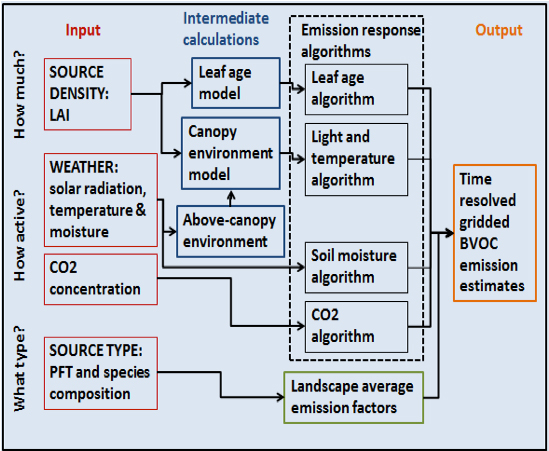
\includegraphics[width=\textwidth]{Figures/MEGANmodel_img.jpg}
      \caption{MEGAN schematic, copied from \citet{Megan_Website}}
      \label{ch_HCHO:fig:megan_schematic}
    \end{figure}

    MEGAN output in Australia is adversely affected by poor emission factor estimation, which is based on plant type classifications (PFTs) and local conditions like soil moisture and weather. 
    An example can be seen in \citet{Muller2008} where MEGAN overestimates isoprene in northern Australia.
    Underestimates of monoterpenes emissions are also seen from MEGAN (TODO: ask Jenny what other paper showed this?), which may be due simply to underestimated emission rates for many Eucalypt species \citep{Winters2009}.
    
\section{GEOS-Chem HCHO simulation}
\label{ch_HCHO:sec:modelHCHO}
  \subsection{Run comparisons}
  
    At the surface level, GEOS-Chem output of HCHO does not differ much between runs with or without the Unified Chemistry eXchange (UCX). 
    Figure \ref{ch_HCHO:fig:HCHOsurfUCXcomparison} shows an example of the surface level HCHO amounts with and without UCX turned on.
    The differences do not exceed 3\% over Australia on this day (1st of January, 2005).
    
    \begin{figure}[!htbp]
      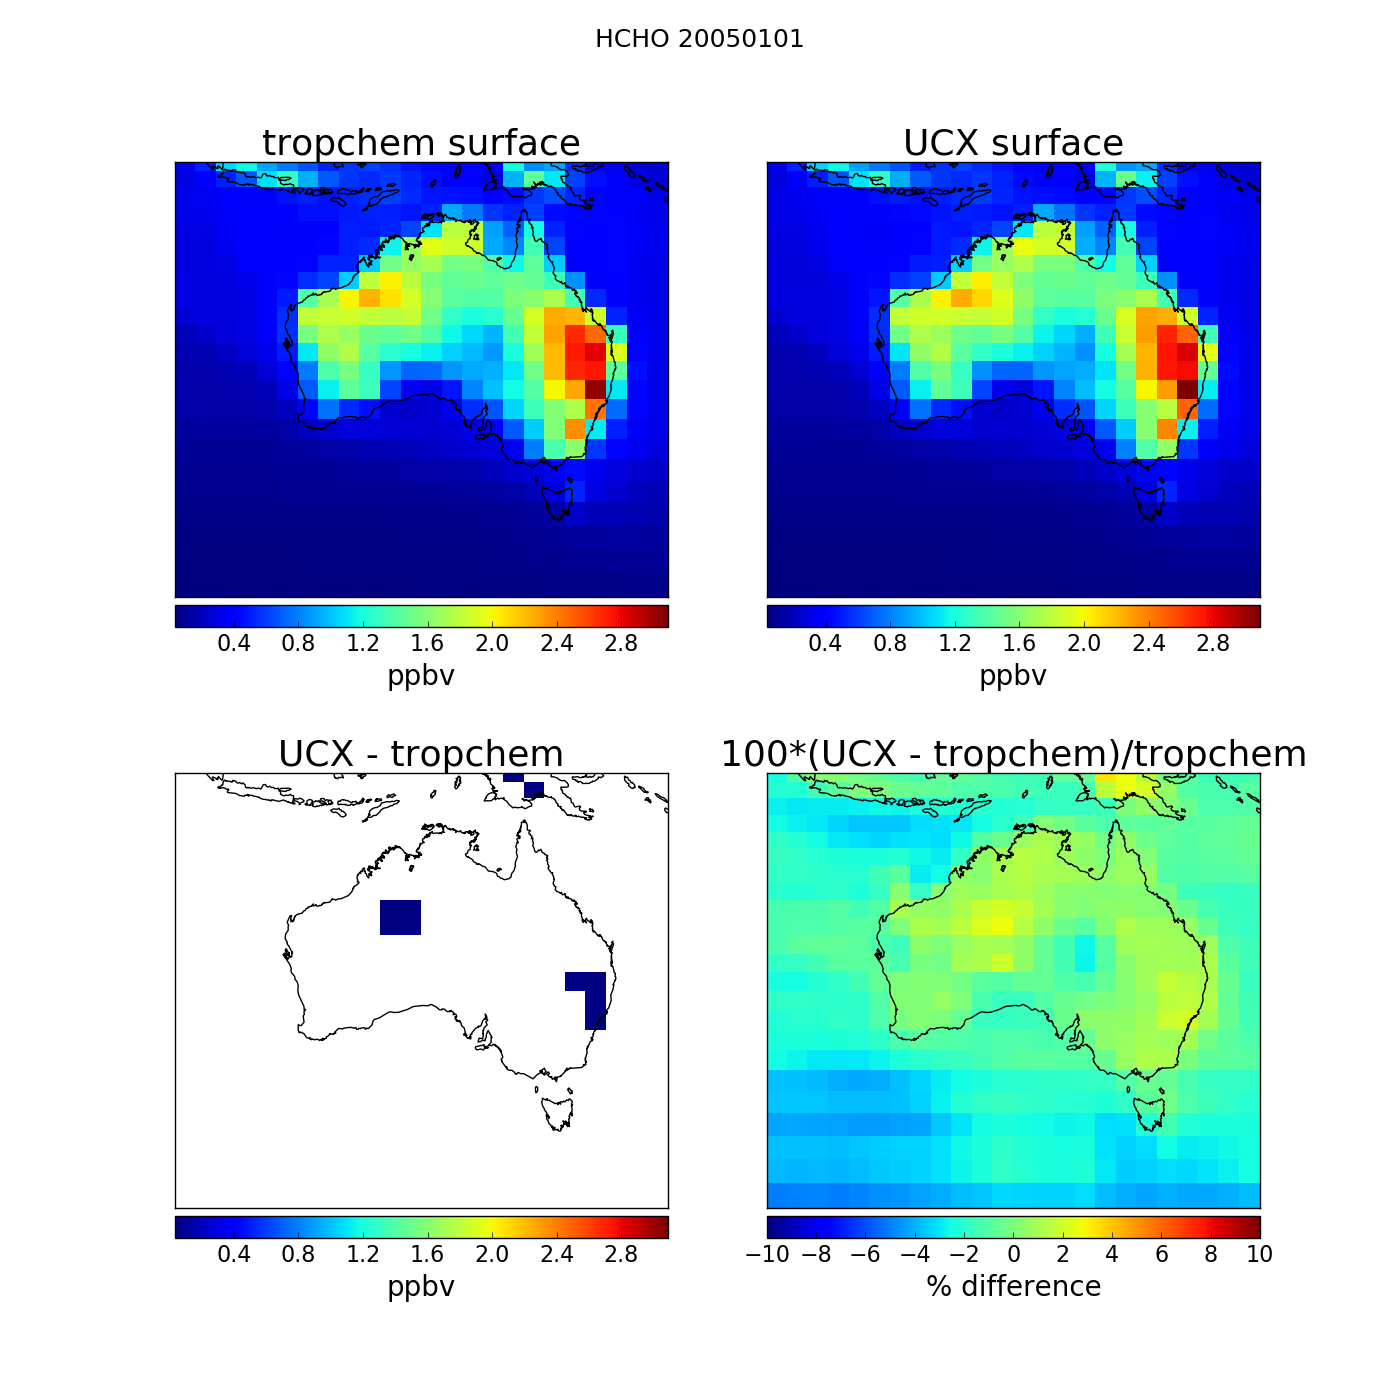
\includegraphics[width=\textwidth]{Figures/HCHO/tropchem_hcho_20050101.png}
      \caption{Surface HCHO simulated by GEOS-Chem with UCX (top left), and without UCX (top right), along with their absolute and relative differences(bottom left, right respectively).
      Amounts simulated by GEOS-Chem on the 1st of January, 2005.}
      \label{ch_HCHO:fig:HCHOsurfUCXcomparison}
    \end{figure}
%----------------------------------------------------------------------------------------
%	SECTION
%----------------------------------------------------------------------------------------  
\section{Satellite HCHO measurements}
\label{ch_HCHO:sec:satelliteHCHO}
  \subsection{Satellite Retrievals}
    Satellites remotely sense atmospheric trace gases through irradiance measurements of solar light which has reflected off the earth's surface. 
    These irradiances are affected by gases which exist along the reflected path of light between the detector, earth, and sun. 
    The irradiance is then used to estimate how much of a particular gas exists along this path, which gives us an estimate which is called a slant column (SC).
    The retrieved SC of a particular gas (or species) can be transformed into a vertical column (VC) by scaling the path length in conjunction with accounting for the trace gas' light scattering properties.
    The scaling coefficient created to transform from SC to VC is called the Air Mass Factor (AMF).

    One satellite is NASA's Earth Observing System's (EOS) Aura, which houses the Ozone Monitoring Instrument (OMI), a near-UV/Visible Charged Coupled Device (CCD) spectrometer.
    Aura orbits the earth in a polar sun-synchronous pattern, circling the earth on a plane coincident with the sun and the poles. 
    OMI measurements are used to map several atmospheric trace gases, including NO$_2$, SO$_2$, BrO, HCHO, O$_3$, and aerosols.
    OMI measurements occur from right to left on a band covering 115$^{\circ}$, resulting in swaths of around 2600~km, with pixel sizes from 13x24~km$^2$ at nadir to 26x135~km$^2$ at the swath edges \citep{Abad2015}.
    The swaths cover Earth daily, although half of these are at night time and contain no useful near-UV/Visible information.
    From here on the word pixel is used to describe one data point retrieved by OMI, which will be located by latitude and longitude within OMI's data product.
    
    Atmospheric HCHO can be measured using Differential Optical Absorption Spectroscopy (DOAS), as long as trace gases with similar features near the same wavelength are accounted for.
    TODO: Go through Lee2005 or Volkamer2005 and detail the DOAS Retrieval of HCHO.
    A DOAS fit determines the total column amount of a trace gas along the path that the instrument views.
    This uses the Beer-Lambert law where radiance is reduced as light travels through a medium.
    The full method details for slant column retrieval by OMI are outlined in section \ref{ch_HCHO:sec:OMI_BOAS}.
    
    Uncertainty in a single pixel for OMI is quite high, roughly the same magnitude as HCHO measurements.
    Figure \ref{ch_HCHO:fig:eightDayUncertainty} shows uncertainty over Australia after one and eight days of averaging at 0.25$^{\circ}$ longitude by 0.3125${\circ}$ latitude.
    There are several methods of calculating this, one of which is used here and compared against the provided uncertainty (TODO) as shown in Section \ref{ch_HCHO:sec:OMIuncertainty}.
    If we assume the uncertainty is random error, and not bias introduced through calculation techniques, then we are able to reduce the uncertainty through averaging.
    Random error can be reduced by either temporal or spatial averaging, decreasing uncertainty by a factor of $1/\sqrt{N}$ where N is the number of observations being averaged.
    
    \begin{figure}[!htbp]
      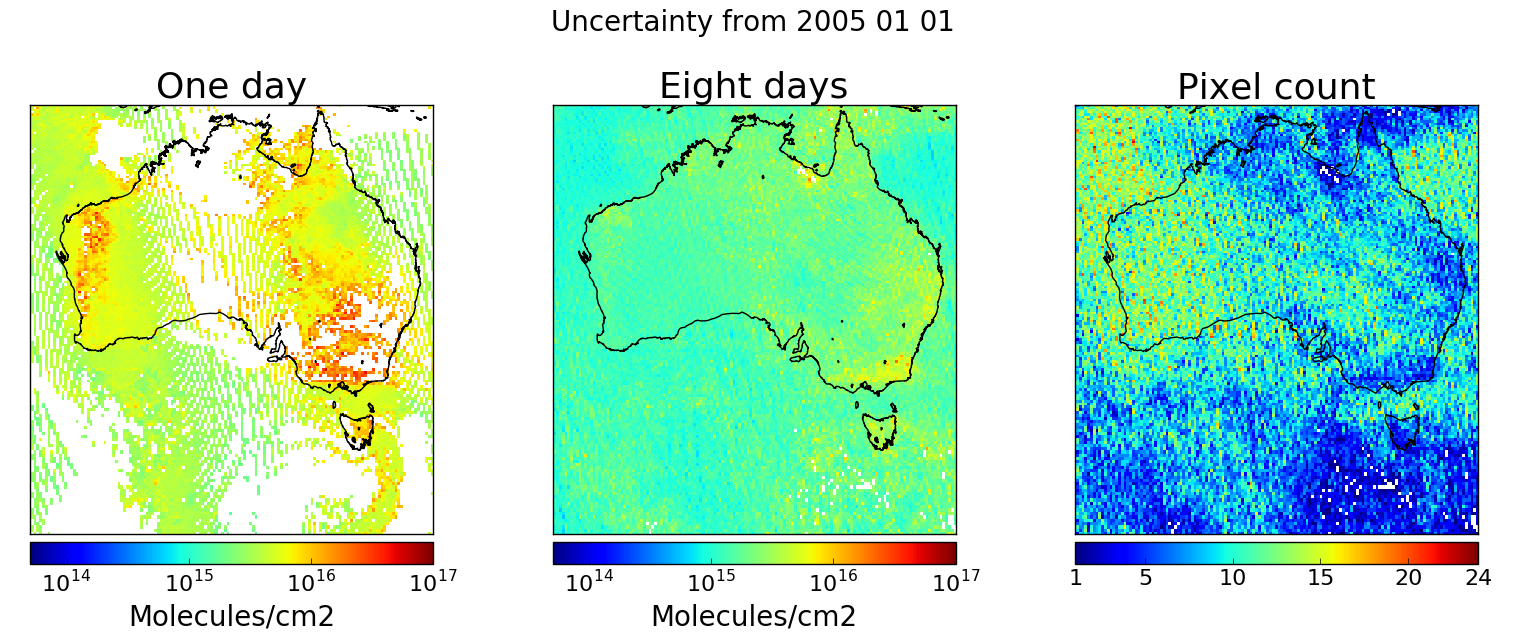
\includegraphics[width=0.7\textwidth]{Figures/HCHO/Uncertainty.png}
      \caption{%
	      OMI uncertainty before and after gridding and averaging 8 days from Jan 1 2005 to Jan 8 2005.
	      The third panel shows the number of pixels in each grid box after 8 days of averaging, before accounting for fire.
      }
      \label{ch_HCHO:fig:eightDayUncertainty}
    \end{figure}
    
  \subsection{OMI Algorithm BOAS}
    \label{ch_HCHO:sec:OMI_BOAS}
    The following information comes from the OMHCHO dataset documentation at \citet{Kurosu2014} and \citet{Chance2002}.
    The method of HCHO total column retrieval depends heavily on measured solar radiation.
    Radiance is directional radiant flux, expressed in Watts per square metre per steradian (a unit of angle used in three dimensional geometry).
    Irradiance is radiant flux received by a surface, expressed in watts per square metre.
    An OMI granule is the sunlit portion of an orbit (one day).
    
    The BOAS algorithm used by OMI is as follows.
    Slant column abundance can be determined by fitting measured radiance (I) at particular wavelengths ($\lambda$), using modelled absorption cross sections ($\sigma$), effective albedo (A) including Rayleigh scattering, a correction for the Ring effect (c$_R\sigma_R$), and a closing polynomial (coefficents c$_0$-c$_3$).
    \begin{equation}
      \label{ch_HCHO:eqn:BOAS_HCHO}
      I(\lambda)  = A I_0 \exp {\left( - \Sigma_i S_i \sigma_i \right) } + c_R\sigma_R + c_0 + c_1(\sigma-\bar{\sigma}) + c_2(\sigma - \bar{\sigma})^2 + c_3(\sigma - \bar{\sigma})^3 
    \end{equation}
    
    For HCHO, absorption cross sections and number densities for interfering gases are determined beforehand.
    This is due to HCHO being so optically thin and interferences must be accounted for precisely \citep{Chance2002}.
    
    In version 3.0 of the OMI satellite data retrievals, HCHO is determined using the spectral window $328.5$~nm$ - 356.5$~nm. 
    The algorithm used is based on direct fitting of radiances and irradiances.
    An OMI radiance measurement over the remote Pacific ocean is used instead of an irradiance measurement.
    This means that the slant columns ($\Omega_S$) are actually the difference with respect to the radiance reference column ($\Omega_{S_0}$).
    
    The model that is fitted to the measurements is made up of the radiance reference attenuated by HCHO contributions, inelastic (rotational Raman) scattering, and interferences from ozone, NO$_2$, BrO, and the O$_2$-O$_2$ collision complex.
    It includes additive and multiplicative closure polynomials and parameters for spectral shift and squeeze, and an undersampling correction and ``common mode'' spectrum.
    The spectral fitting results in HCHO slant columns, which are converted to vertical columns through a look-up table of AMFs (see section \ref{ch_HCHO:sec:satelliteHCHO:AMFs})
    Undersampling is a problem caused by the wavelength resolution of the instrument.
    Nyquist theorem requires that the sampling rate be at least twice the highest frequency of the signal in order to uniquely reconstruct it, otherwise the signal is undersampled (contains errors).
    
    There are three main stages in the algorithm:
    \begin{enumerate}
     \item Radiance wavelength calibration, finding the optimum wavelength registration for a representative swath of radiance measurements, and determination of a common wavelength grid for auxiliary data (molectular reference cross sections, etc.).
     \item On-line common mode spectrum calculation from residual fits of the central portion of the orbit. 
     This accounts for systematic features not considered in the semi-empirical model.
     \item Nonlinear least-squres fitting of all swath lines in the OMI granule. 
     Fitting is performed individually for the 60 cross-track pixels in each swath line.
    \end{enumerate}
    
    Cross-track striping is systematically higher or lower column values along a whole track.
    Several methods are used to reduce cross-track striping of the HCHO columns.
    These include soft calibration, which is the use of a daily radiance reference, and outlier screening in the fitting residuals.
    
  \subsection{Optical Depth (\texorpdfstring{$\tau$)}{t}}
    \label{ch_HCHO:sec:satelliteHCHO:OpticalDepth}
    
    Optical Depth, also called optical thickness, is the natural logarithm of the ratio of incident radiant power to transmitted radiant power through a material.
    In the atmosphere we are interested in the optical depth of various chemical species, and we use incoming solar radiation to determine this.
    The difference between solar radiation at the top of the atmosphere and the Earth's surface defines the atmospheric optical depth along the path of observation.
    \begin{equation*}
      \tau = \ln{\frac{\phi_e^i}{\phi_e^t}}
    \end{equation*}
    where $\phi_e^i$ is radiant flux seen at the earth surface, $\phi_e^t$ is the solar radiant flux which arrives at the top of the atmosphere.
    In the atmosphere, optical depth can be due to several factors including scattering, chemical absorbance, and aerosols.
  
  \subsection{Scattering}
    \label{ch_HCHO:sec:satelliteHCHO:scattering}
    Rayleigh and Mie scattering describe two kinds of particle effects on radiation passing through a medium. 
    Rayleigh scattering is heavily wavelength dependent, and is the dominant form of scattering from particles up to roughly one tenth of the wavelength of the light.
    Mie scattering is more dominant from larger particles, and has less wavelength dependence. These scattering functions are described in detail at (TODO:section? reference?).
    
    The effects of scattering are what gives us the information about substances in the atmosphere.
    The different particals and gases in the air have various properties which affect remote sensing devices such as a satellite, making them more or less sensitive at certain altitudes for detecting various species \citep[e.g.]{Martin2002b}.
    
    
  \subsection{Absorption cross section and number density}
    \label{ch_HCHO:sec:satelliteHCHO:crosssection}
    TODO: Fill in this section, describe cross sections.
    
    
    $\tau$ can be described using the attenuation cross section (the attenuation coefficient divided by its number density), with the following relation:
    \begin{equation*}
      \tau = \int_0^l \alpha(z)\eta(z)\mathrm{d}z
    \end{equation*}
    where $\alpha(z)$ and $\eta(z)$ represent absorption cross section in m$^2$ molecule$^{-1}$, and number density in molecules m$^{-3}$ respectively, and l represents the length of the path the light is travelling through. 
  
  
  \subsection{Air Mass Factors}
    \label{ch_HCHO:sec:satelliteHCHO:AMFs}
    DOAS retrieval columns are an integration of a trace gas over the instrument's viewing path, in order to convert this total to a vertically distributed column a few assumptions and estimates are required. 
    The vertical profile of a trace gas is assumed or estimated via a CTM, while its' scattering and radiative properties are calculated at all altitudes using an RTM. 
    These properties are combined into a single array called the AMF which can be combined with a SC to produce a VC.
    AMFs are unique to each trace gas and due to their complexity and the influence of cloud cover they remain one of the larger error sources in remote sensing of BVOCs \citep{Palmer2001,Millet2006}).
    
    The latest OMI algorithm uses a shape factor determined from GEOS-Chem using 47 vertical levels at monthly temporal resolution and 2$^{\circ}$ latitude by 2.5$^{\circ}$ longitude horizontal resolution \citep{Abad2015}.
    The GEOS-Chem model has been substantially updated since then, and using the more recent version $V10.01$ to recalculate the AMF is performed within this thesis, details are shown in section \ref{ch_HCHO:sec:satelliteHCHO:CalculationOfVC}.
    
    The vertical distribution of a trace gas determined by CTM is independent of the vertically dependent observation sensitivity provided by RTM, which prevents model contamination of remotely sensed data.
    Two examples of this are GOME-2 products on the MetOp-A satellite (\url{http://atmos.caf.dlr.de/gome/product_hcho.html}) and OMI products which use IMAGESv2 combined with LIDORT and GEOS-Chem with LIDORT for product processing respectively \citep{Chance2002, Abad2015}.
    The recalculation of OMI AMFs is explained in section \ref{ch_HCHO:sec:satelliteHCHO:CalculationOfVC}).
    
    Calculations of the AMF performed by different groups tend to agree fairly well, as long as all the apriori and ancilliary data is similar.
    Large differences can occur depending on the apriori vertical profile, trace gas concentrations, and cloud properties \citep{Lorent2017}.
    Choice of RTM and interpolation operations have a relatively small affect compared to the assumed state of the atmosphere, with high structural uncertainty introduced at this stage of AMF calculation - as shown in \cite{Lorent2017}.

    Code for recalculating AMFs using satellite swaths and modelled aerosol optical depths and gas profiles can be found at \url{http://fizz.phys.dal.ca/~atmos/martin/?page_id=129}. 
    The original method for HCHO is layed out in \cite{Palmer2001}, with modifications for clouds \citep{Martin2002NO} and use of the LIDORT RTM \citep{Spurr2002} is described by \cite{Martin2003NO}.
    This code does not work as is when using OMI satellite data, and requires modifications as first performed by Luke Surl at Edinburgh University.
    Additionally dr. Surl acquired the tropopause heights averaged within satellite overpass times output by GEOS-Chem with modifications to the model diagnostic (ND51).
  
  \subsection{OMI HCHO data products}
    OMI Data products are generally classed into several categories, level 0 through to level 3. Level 0 products are sensor counts and orbital swath data, level 1B data calibrates and geo-locates the level 0 data. Level 2 products additionally have temporal, spatial, solar, and viewing geometry information, as well as quality flags.
    To create level 2 data slant column density is determined and then translated into vertical column density using an AMF calculated through radiative transfer models. Level 3 data is a temporally aggregated version of the this, for instance monthly or yearly averages.
    
    In order to filter fire or anthropogenic influence on HCHO data one generally requires the level 2 data along with extra data such as MODIS and AATSR fire counts, and national or regional industrial emissions estimates.
    %The lead scientist for level 1B data products is Dr. M. Dobber.
  
  \subsection{HCHO Vertical Column Calculation}
    \label{ch_HCHO:sec:satelliteHCHO:CalculationOfVC}
    
    The method used here largely follows that of \citet{Palmer2001}.
    The Beer-Lambert law of extinction allows spectroscopic measurement of absorbing chemical species (absorbers) in the atmosphere:
    \begin{equation} \label{ch_HCHO:eqn:beerlambert}
      I_B = I_{B_0} e^{-\tau_s}
    \end{equation}
    where I$_B$, I$_{B_0}$ is backscattered intensity with and without the absorber respectively, and $\tau_s$ is the optical thickness of the slant column absorber (see section \ref{ch_HCHO:sec:satelliteHCHO:OpticalDepth}).

    The AMF is needed to transform the slant column, as viewed by the satellite, into a vertical column:
    \begin{equation} \label{ch_HCHO:eqn:AMFratio}
      AMF = \frac{\Omega_s}{\Omega_v} = \frac{\tau_s}{\tau_v}
    \end{equation}
    where s and v subscripts refer to slant and vertical values, while $\Omega$ represents a column of absorber in molecules cm$^{-2}$.

    In the absence of atmospheric scattering a simple geometric AMF can be defined as a function of the solar zenith angle. 
    The solar zenith angle ($\theta_s$) and the satellite viewing angle ($\theta_v$) are shown in image \ref{ch_HCHO:fig:zenithangle}.
    However, in the UV-VIS region of the spectrum, Rayleigh and Mie scattering (see section \ref{ch_HCHO:sec:satelliteHCHO:scattering}) must be accounted for.
    Using equations \ref{ch_HCHO:eqn:beerlambert} and \ref{ch_HCHO:eqn:AMFratio} gives us an expression for the AMF which includes scattering:
    \begin{equation} \label{ch_HCHO:eqn:AMFscattering}
      AMF = \frac{\ln{I_{B_0}}-\ln{I_B}}{\tau_v}
    \end{equation}

    \begin{figure}[!htbp]\begin{center}
      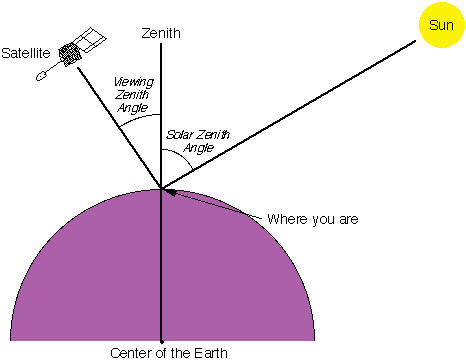
\includegraphics[width=0.6\textwidth]{Figures/ZenithAngles.png}
      \caption{Solar and viewing zenith angles, image copied from \citet{SZA_Image}, originally from a NASA website.}
      \label{ch_HCHO:fig:zenithangle}
    \end{center}\end{figure}

    We use $\nabla I = I_B - I_{B_0}$ to represent the change in intensity due to the absorber. Note that for optically thin absorption, $\nabla I / I_B << 1$, and we can use:
    \begin{equation} \label{ch_HCHO:eqn:AMFthin}
      AMF = \frac{\ln{ \left( 1 - \frac{\nabla I}{I_B} \right)} }{\tau_v} \approx \frac{ - \frac{\nabla I}{I_B} }{\tau_v}
    \end{equation}
    $\nabla I$ can also be expressed as the integral of the absorption slices over optical depth increments: 
    \begin{equation*}
      \nabla I = \int_0^{\tau_v}{\frac{\partial I_B}{\partial \tau} \mathrm{d}\tau}
    \end{equation*}
    which can be placed into equation \ref{ch_HCHO:eqn:AMFthin}:
    \begin{equation*}
      AMF \approx \frac{-1}{\tau_v} \int_0^{\tau_v}{\frac{\partial \ln{I_B}}{\partial \tau} \mathrm{d}\tau}
    \end{equation*}
    and rewritten as:
    \begin{equation} \label{ch_HCHO:eqn:AMFcross}
      AMF = \frac{-1}{\tau_v} \int_0^\infty {\frac{\partial \ln{I_B}}{\partial \tau} \alpha(z)\eta(z)\mathrm{d}z}
    \end{equation}
    where $\alpha(z)$ and $\eta(z)$ represent absorption cross section in m$^2$ molecule$^{-1}$, and number density in molecules m$^{-3}$ respectively. This uses the attenuation cross section relationship to optical depth (see section \ref{ch_HCHO:sec:satelliteHCHO:crosssection}).

    To represent an average cross section weighted by the absorbing species' vertical distribution, intended to account for temperature and pressure dependence of $\alpha(z)$, $\alpha_e$ is defined as:
    \begin{equation*}
      \alpha_e = \frac{1}{\Omega_v} \int_0^\infty \alpha(z) \eta(z) \mathrm{d}z
    \end{equation*}

    This is the same as $ \tau_v = \Omega_v \alpha_e $, which we can place into equation \ref{ch_HCHO:eqn:AMFcross} to obtain:
    \begin{equation*}
      AMF=-\int_0^\infty{ \frac{\partial \ln{I_B}}{\partial \tau} \frac{\alpha(z)}{\alpha_e} \frac{\eta(z)}{\Omega_v} \mathrm{d}z }
    \end{equation*}

    Defining w(z) as the scattering weights describing the sensitivity of the backscattered spectrum to the abundance of an absorber at altitude z:
    \begin{equation}
      \omega(z) = -\frac{1}{AMF_G} \frac{\alpha(z)}{\alpha_e} \frac{\partial \ln{I_B}}{\partial \tau}
    \end{equation}
    and vertical shape factor S$_z$(z) representing a normalized vertical number density profile: 
    \begin{equation} \label{ch_HCHO:eqn:ShapeFactor}
      S_z(z) = \frac{\eta(z)}{\Omega_v}
    \end{equation}
    
    Now the AMF can be expressed as
    \begin{equation} \label{ch_HCHO:eqn:AMFintwSdz}
      AMF = AMF_G \int_0^\infty w(z) S_z(z) \mathrm{d}z
    \end{equation}
    It's worth noting that in the OMI satellite product, the provided $\omega(z)$ term does not include the $\frac{1}{AMF_G}$ term and a the calculation in equation \ref{ch_HCHO:eqn:AMFintwSdz} does not use the $AMF_G$ term.
    This is not noted in any of the papers which recalculate the AMF from the OMI product, due to them recalculating the $\omega$ term themselves with a radiative transfer model such as LIDORT.
    
    For this equation $\omega$ is a function of atmospheric scattering which can be calculated using an RTM to determine the absorption cross section and optical thickness along the path.
    S$_z$(z) can be calculated using an apriori vertical profile, which may be sourced from any atmospheric chemistry model.
    Note that for level two non-gridded OMI satellite HCHO total column data, the w(z), S$_z$(z), and AMF$_G$ are all provided.
    
    Mie scattering and clouds can complicate the calculation of $\omega$(z), however tables of values for this function at various parameter inputs can be used with modeled vertical shape factors for local AMF calculations.
    
    Using the vertical coordinate sigma ($\sigma$), which is related to pressure (P) by $P=\sigma \left( P_S - P_T \right) + P_T$, where subscripts S and T represent earth surface and top of the atmosphere respectively.
    The hydrostatic relation $P = - \rho_a g z$, with $\rho_a$, g, being density of air, gravity, respectively lets us switch to the sigma coordinate using:
    \begin{align*}
      \rho_a g z & = \sigma \left( P_S - P_T \right) + P_T \\
      \mathrm{d}\sigma  & = - \frac{ \rho_a g }{ P_S - P_T } \mathrm{d}z
    \end{align*}
    
    Substitution into \ref{ch_HCHO:eqn:AMFintwSdz} gives AMF using the sigma coordinates:
    \begin{equation} \label{ch_HCHO:eqn:AMFintwSdsigma}
      AMF = AMF_G \int_0^1 w(\sigma) S_\sigma(\sigma) \mathrm{d}\sigma
    \end{equation}
    Where S$_\sigma$ is defined as a vertical shape factor representing a normalised mixing ratio:
    \begin{equation}
      S_\sigma (\sigma) = \frac{\Omega_a}{\Omega_v}C(\sigma)
    \end{equation}
    where $\Omega_a$ is the vertical column of air and C($\sigma$) is the mixing ratio of the absorber.
    This normalised shape factor is dimensionless.
    This can be useful when running global atmospheric models as the ground altitude is always at $\sigma=1$ and we need not worry about topography.
    
    When comparing satellite observations to a chemical model, one needs to recalculate the satellite AMF using their own modelled vertical gas profiles as the a-prior shape factor in order to remove any total column bias which may be due to the satellite's apriori.
    Another way of removing this bias is through deconvolution (TODO: EQNS) of the averaging kernal (AK) of the satellite instrument.
    The AK represents sensitivities to each species at multiple altitudes through the atmosphere and in the case of OMI, can be approximated from the w(z) function as follows:
    \begin{equation} \label{ch_HCHO:eqn:AKfromw}
      AK(z) = \frac{\omega(z)}{AMF}
    \end{equation}
    Note that this is an approximation for the OMI product, which does not include the AK but does include the $\omega$ and AMF, as explained in \citet{Abad2015}.
    
  \subsection{Uncertainty in OMI total columns}
  \label{ch_HCHO:sec:OMIuncertainty}
    Provided with the OMI product is the measurement of uncertainty in each pixel, calculated by SAO from the backscattered solar radiation fit \citep{Abad2015,Abad2016}.
    BIRA use another method, and calculate the standard deviation of HCHO over the remote pacific ocean as the uncertainty \citep{DeSmedt2012, DeSmedt2015}.
    In the remote pacific, it can be assumed that HCHO variations are weak, with concentrations remaining steady in the short term ($\sim 1$ month).
    This means the standard deviation over this region can be used as a proxy for determination of the instrument error.
    For an analysis of the uncertainty in the recalculation of the OMI HCHO vertical columns see section \ref{ch_HCHO:sec:OMI_uncertainty_calculation}.
    
  \subsection{Reference sector correction for comparison of products to various models}
    HCHO products from OMI and SCIAMACHY both use a median daily remote pacific ocean radiance reference spectrum, over 15$^{\circ}$S-15$^{\circ}$N, 140$^{\circ}$-160$^{\circ}$W where it is assumed that the only significant source of HCHO is methane oxidation \citep{DeSmedt2008,Barkley2013,Kurosu2014}.
    Since this oceanic background is used instead of a solar irradiance spectrum, in order to compare the output against different models, the vertical columns need to be corrected by an absolute amount.
    The corrected vertical column ($\Omega_V$) is calculated as the slant column ($\Omega_S$) minus the reference slant column ($\Omega_{S_0}$) multiplied by the AMF, plus the modelled reference sector column ($\Omega_{V_B}$):
    \begin{equation*}
      \Omega_V = \frac{ \left( \Omega_S - \Omega_{S_0} \right) }{ AMF } + \Omega_{V_B}
    \end{equation*}
    This method is used in various papers, including \citet{DeSmedt2008, DeSmedt2012, DeSmedt2015, Barkley2013, Bauwens2016}.
    
    Recently this correction was expanded (for OMI data) to include latitudinal and instrument track influence by \citet{Abad2015}.
    The updated correction is explained in detail in section \ref{ch_HCHO:sec:RSC}.
    
%----------------------------------------------------------------------------------------
%	BVOC FROM HCHO SECTION
%----------------------------------------------------------------------------------------
\section{Recalculating HCHO from satellite(OMI) data over Australia}
\label{ch_HCHO:sec:creatinginventory}

  \subsection{Process Outline}
    First satellite slant columns of formaldehyde for the years January 1st, 2005 - April 1st, 2013 are downloaded from NASA.
    The data set used is from the Ozone Monitoring Instrument (OMI) on board the Aura satellite, as it has data for the entire time line and sufficiently covers the southern hemisphere.
    This data is first quality assured and undergoes basic analysis and filtering criteria as is done in several other studies \citep[eg.]{Marais2012, Barkley2013, Bauwens2016, Zhu2016}.
    This filtering removes cloudy and uncertain data points, along with instrument problems such as the OMI row anomaly (see section \ref{ch_HCHO:sec:OMIFiltering}.
    A full account of the filters used when reading OMI satellite data is given in section \ref{ch_HCHO:sec:OMIFiltering}.
    
    In order to reduce uncertainty and increase the utility of the satellite data we regrid it from pointwise single time data points to 8-day averages on a latitude longitude grid which matches our model input and output grid spacing. 
    Using the 8-day average reduces the uncertainty in each datapoint significantly, TODO: citet marais and barkley uncertainty improvements, details of the uncertainty estimations is shown in section \ref{ch_HCHO:sec:OMI_uncertainty_calculation}.
    %Another example is shown in \citet{Vigouroux2012} where uncertainty near a specific location is lowered by averaging daily within a 500km radius and only using the meaned data when there are at least 20 good values.
    
    Once the slant columns are quality filtered and gridded, additional data sources need to be used to account for anthropogenic and pyrogenic sources of HCHO.
    MODIS fire counts are used in conjunction with NO$_2$ enhancements (also measured by satellite) to remove data points which may be affected by fires. 
    TODO:If it is easier to use OMI smoke smoke aaod I'll do it that way instead of using the NO2, write here if that is the case.
    One possible solution to anthropogenic filtering is the national pollution index (TODO:cite:\verb|http://www.npi.gov.au|) which contains industrial HCHO and NO$_X$ emissions from 2003 to 2014.
    This has a negative affect on uncertainty, as fewer measurements are averaged over the 8-days. 
    The affect of the fire filtering on uncertainty, and how many points are removed is shown in section \ref{ch_HCHO:sec:filteringfires}.
    
    Each satellite slant column measurement is corrected by some amount, based on the divergence from a modeled reference sector.
    The reference sector correction method corrects for several problems, however it introduces some apriori model influence.
    One of the problems removed through this correction method is instrument degradation, which can introduce bias over time.
    Another is the possible influence of varying dead/hot pixel masks across 2-D detector arrays such as OMI \citep{DeSmedt2015}.
    This method also corrects for the errors introduced through correlations between BrO and HCHO absorption cross sections, which are especially significant at high latitudes \citep{Abad2015}.
    
    The reference sector we use is defined over the pacific ocean at 140 to 160$^{\circ}$W and 90$^{\circ}$N to 90$^{\circ}$S, as in \citet{Abad2015}.
    HCHO concentrations are assumed to be at background levels over the pacific ocean, with their only source being CH$_4$ oxidation.
    A correction for each instrument pixel is created based on the difference between the background HCHO measurements from OMI and the GEOS-Chem modelled HCHO columns within the reference sector.
    This correction is calculated daily and applied to all good pixels based on their latitude.
    The full process for this is shown in section \ref{ch_HCHO:sec:RSC}.
    
    In order to visualise and analyse satellite column data it is generally transformed into vertical columns. 
    This is done using AMF calculations as shown in section \ref{ch_HCHO:sec:satelliteHCHO:CalculationOfVC}.
    Taking the biogenic slant columns, scattering weights, and apriori estimates of HCHO vertical profiles we determine vertical HCHO column amounts.
    This is an in depth process involving radiative transfer modelling in order to work out satellite sensitivities at various altitudes, as well as the effect from the local HCHO profile on those sensitivities.
    Several of these required data are available from the satellite data products, including the scattering weights and the zenith angles required to determine an AMF at any particular measured point.
    In this work the shape factor is recalculated from GOES-Chem, with the associated OMI per-pixel scattering weights unchanged. 
    The satellite shape factor is replaced by GEOS-Chem's overpass time simulated HCHO profile, normalised and saved daily along with air density.
    
    When comparing satellite measurements against models it is important to recognise the impact of the apriori shape factor on the total column values.
    This is due to the sensitivity of instruments varying vertically through the atmosphere, and how the simulated distribution of HCHO is accounted for.
    In order to remove a possible bias caused by systematic differences between the old model and the current model, the shape factor used by the satellite is replaced using the profile from the current model before satellite total columns are recalculated (generally using equation \ref{ch_HCHO:eqn:AMFintwSdz}).
    Both the shape factor and scattering weights of the satellite are recalculated using a combination of GEOS-Chem apriori profile information and satellite measurement data using code initially written by dr. Paul Palmer, which calculates the AMF after running the LIDORT radiative transfer calculations to determine apriori scattering, this is explained fully in section TODO: and how it's used is shown in section \ref{ch_HCHO:sec:PPCode}.
    Without performing this step a bias between modeled and measured total column values may be due to an apriori rather than actual chemistry or measurements.

  \subsection{Quality filtering OMI HCHO slant columns}
    \label{ch_HCHO:sec:OMIFiltering}
    TODO: Quality flags and cloud cover metric uses, and discussion, along with statistics like how many datapoints are removed.
    
    The OMI dataset has a quality flag which can be used to remove unlikely or poor satellite measurements.
    The states represented by this quality flag are shown in table \ref{ch_HCHO:tab:OMIQualityFlag} which is taken from \citet{Kurosu2014}.
    Filtering bad or missing measurement pixels is preformed prior to any other filtering, this includes the datapoints affected by the row anomaly.
    This anomaly (\url{http://projects.knmi.nl/omi/research/product/rowanomaly-background.php}) affects radiance data at particular viewing angles, corresponding to a row on the CCD detectors, and is dynamic over time.
    The slant columns affected are flagged and easy to remove before further processing.
    
    Clouds have various detrimental effects on slant column uncertainty and AMF calculation, so the cloudy data needs to be filtered.
    Any pixel with a cloud fraction of greater than 40\% is also removed, after the pixel is used in determining the reference sector correction, as is done in \citet{Abad2015, DeSmedt2015}.
    %In \citet{???} (TODO: find this paper), pixels with more than half of the backscattered intensity from the cloudy sky fraction are removed, in effect removing pixels with more than ~40\% cloud fraction before calculating the AMF for NO$_2$ slant columns.
    Another way this has been performed is to remove pixels where the AMF lies outside a certain range: \citet{Martin2002} filter AMFs below 0.5 in order to remove the effects of heavy cloud and optical thickness.
     
    \begin{table}
      \caption{OMI quality flag values table from \citet{Kurosu2014}}
      \begin{tabular}{  l  l  p{10cm} }
        \hline
        \textbf{Value} & \textbf{Classification} & \textbf{Rational} 
        \\ \hline
        0 & Good & Column value present and passes all quality checks; data may be used with confidence. 
        \\ \hline
        1 & Suspect & Caution advised because one or more of the following conditions are present: 
          \begin{itemize}
            \item Fit convergence flag is $<$ 300 but $>$ 0: Convergence at noise level
            \item Column $+ 2 \sigma$ uncertainty $<$ 0 $<$ Column $ + 3 \sigma $ uncertainty
            \item Absolute column value $>$ Maximum column amount (1e19 molec cm$^{-2}$)
          \end{itemize}
        \\ \hline
        2 & Bad & Avoid using as one of the following conditions are present: 
          \begin{itemize}
            \item Fit convergence flag is $<$ 0 : No convergence, abnormal termination
            \item Column $+ 3 \sigma$ uncertainty $<$ 0
          \end{itemize}
        \\ \hline
        $<0$ & Missing & No column values have been computed; entries are missing
        \\ \hline
      \end{tabular}
    \label{ch_HCHO:tab:OMIQualityFlag}
    \end{table}
    
    The cloud fraction with each pixel is provided with the OMHCHO dataset, however its source is the OMI cloud product, OMCLDO2.
    To give an idea of how much data is filtered out, around 30\% of the pixels which remain after filtering out the bad or missing data are subsequently removed due to cloudiness.
    
    Further filtering is performed to remove the measurements which are most likely to be unrealistic: pixels wit a solar zenith angle greater than 60$^\circ$, and those with column density outside the range $-0.5 \times 10^{16}$ to $10^{17} $~molecules cm$^{-2}$.
    These are similar filters to those applied in (TODO: read \citet{Zhu2016}, add similar justification if succinct).
    This final filter is required due to currently unexplained large negative values which occur in the OMI HCHO product increasingly over time.
    Figure \ref{ch_HCHO:fig:OMI_negative_hist} shows how unfiltered HCHO columns are affected by a small set of highly negative values which heavily affect the mean column amount over any region.
    The histograms here show the negative (left) and positive (right) total column HCHO measurements from a subset of swaths over Australia, on the 18th of March 2013.
    The highly negative values can be seen around the $-10^{19}$~molecules cm$^{-2}$ region.
    
    \begin{figure}[!htbp]\begin{center}
      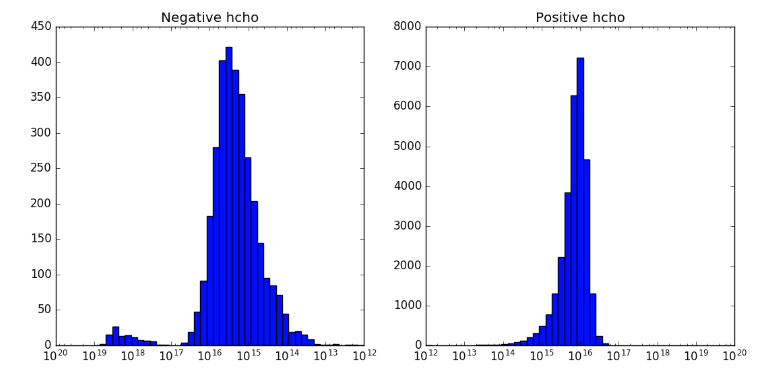
\includegraphics[width=0.7\textwidth]{Figures/AusOMHCHO_Hist_20130318.png}
      \caption{Column density histograms for a subset of OMI swaths over Australia on the 18th of March 2013.
      Negative entries are shown in the left panel, positive in the right, note the different scale between negative and positive panels.}
      \label{ch_HCHO:fig:OMI_negative_hist}
    \end{center}\end{figure}
    
    One final selection of the data is removed prior to calculation and analysis due to instrument sensitivity issues.
    This removed data is based on the latitude of the satellite measurement, high northern and southern latitudes are removed as the effect of both the high solar zenith angle and (over arctic regions) the high albedo cause anomalous readings which are hard to correct.
    The latitudes removed from analysis for OMI satellite data are those outside of $0^\circ \pm 60^\circ$. 
    This is where the satellite measurements are less robust, and often publications will remove this same region (TODO: cites where they did this).
  
    
  \subsection{Reading OMHCHO daily slant columns}
    Each $\sim90$ minutes the AURA satellite sweeps over the sunny side of the planet, with OMI recording roughly 90~k pixels, of which around 50~k -- 80~k are classified as good.
    Each pixel contains several important pieces of data which are needed for recalculation of the HCHO vertical column: the total column of HCHO (molecules cm$^{-2}$), cloud fraction, associated shape factor, AMF, geometric AMF, scattering weights and their vertical altitudes (hPa), viewing zenith angle, solar zenith angle, latitude, longitude, OMI sensor track, main data quality flag, cross track flag, and total column uncertainty.
    All of these data are needed in order to reconstruct the total vertical column using a modelled apriori shape factor rather than NASA's included apriori shape factor.
    Each pixel and it's relevant data are saved in a long list, around $1.1$ million pixels per day.
    As well as the data directly read from the OMI swath files, further information is added to each pixel.
    This is the new AMF calculated through replacing the apriori vertical profile with the newer GEOS-Chem simulated profile, which is described in section \ref{ch_HCHO:sec:recalculating_AMF_description}.
    The shape factors and scattering weights for each pixel lie along a z-axis which is vertically resolved to 47 layers and is shown in figure TODO: make figure showing this stuff and an example profile.
    
    TODO: Show an example of OMI swaths.
    
  \subsection{Regridding to 0.25 by 0.3125 8-day averaged vertical columns}
    
    Regridded OMI HCHO columns from the are based on 14-15 daily swaths of measurements provided by NASA. 
    Each swath contains roughly $9 \times 10^4$ pixels, each of which contains various data including latitude, longitude vertical column HCHO, etc.
    In order to regrid these columns each pixel is mapped into a global grid of 0.25$^{\circ}$x0.3125$^{\circ}$ latitude by longitude (matching GEOS-5 native resolution) which may contain up to 15 entries from a particular day's orbits.
    Total vertical column amounts (both the satellite original and the columns reprocessed as follows) are averaged over each 8 days starting on January 1st 2005.
    
    The process of regridding is performed by first reading all relevent information at each pixel for a single day into a list in python, which is then processed, with the shape factor read from GEOS-Chem output and AMF recalculated, before being saved as a gridded array of total columns and pixel counts.
    The total columns are averaged into each grid box for each day, and eventually averaged over eight day time periods.
    
    TODO: time per regridding and reprocessing:
    This mapping requires some processing time as well as RAM and computer storage space, and has been performed on the National Computing Infrastructure (NCI) supercomputer cluster.
    In order to reprocess one year of swath files, X GB of daily data was downloaded and then transformed into Y GB of 8-day averaged gridded data.
    This takes around 90 minutes per day, and is very parallelisable as each day is completely independent.
    Using N$\times 8$ concurrent processors on NCI's computer cluster running Python allows for very fast reprocessing of our entire timeline.
    As much as possible, processing is done using the HDF-EOS5 format, with GEOS-Chem output being read and processed from bitpunch to HDF-EOS5 prior to reprocessing.
    The scripts to regrid and reprocess the swath data set are available in the supplementary (TODO).
    
  \subsection{Filtering pyrogenic HCHO}
  \label{ch_HCHO:sec:filteringfires}
    TODO: How modis fire counts are used as well as statistics on removed data points.
    
    On board NASA's AQUA satellite, the MODIS instrument is used to detect fire activity.
    The product used here is called MYD14C8H (\citep{Giglio2006}), which looks at fire activity over eight days on a 0.5$^{\circ}$ square grid globally.
    Regridding the product to the native meteorological grid of GEOS5 at 0.25$^{\circ}$ latitude by 0.3125$^{\circ}$ longitude is done in python with an interpolator which maps the values of the new grid rectangles to the value of the nearest grid square.
    An example of the change in resolution is provided in figure \ref{ch_HCHO:fig:modisgridspace}, where the grids are shown over a basic map of Tasmania.
    The direct affect of this interpolation is shown as an example in figure \ref{ch_HCHO:fig:modisinterpolation}, which is showing the regridded MODIS fire count over Australia from January 2005 (avg of first 8 days) in two subplots.
    
    \begin{figure}[!htbp]\begin{center}
      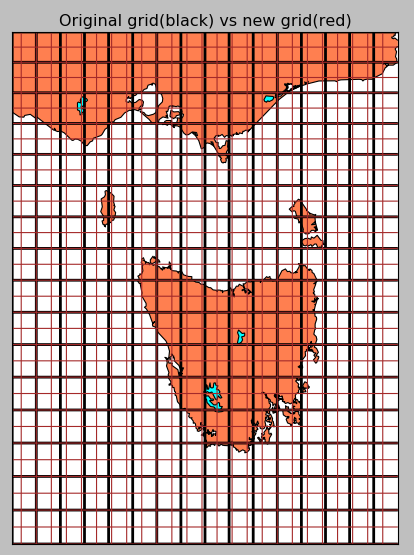
\includegraphics[width=0.7\textwidth]{Figures/MODIS_grid_space.png}
      \caption{Example of grid space change using 0.5x0.5 and 0.25x0.3125 latitude by longitude resolution.}
      \label{ch_HCHO:fig:modisgridspace}
    \end{center}\end{figure}
    
    \begin{figure}[!htbp]\begin{center}
      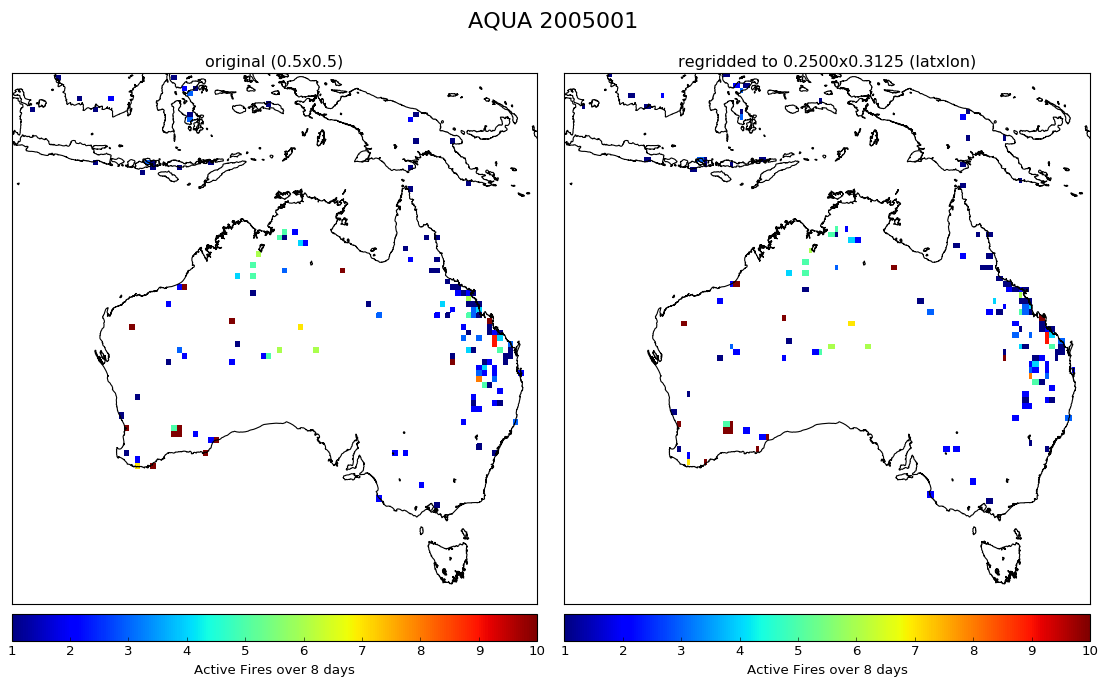
\includegraphics[width=\textwidth]{Figures/MODIS_Regrid_Comparison.png}
      \caption{Example of MODIS 8 day grid interpolation from 0.5x0.5 to 0.25x0.3125 latitude by longitude resolution.
      This example uses MODIS fire counts for 1-8 January 2005.}
      \label{ch_HCHO:fig:modisinterpolation}
    \end{center}\end{figure}
    
    Figure \ref{ch_HCHO:fig:fireexclusionexample} shows an example of the total column HCHO calculated using GEOS-Chem aprioris ($\Omega_{GEOS}$) before and after using the MYD14C8H product to exclude fire influenced pixels.
    (TODO: show time series of how many pixels are removed and discuss if this causes any issues down the line)
    % January 1, 2005 : 113384 / 130295 nan entries before and after fire exclusion within 60 degrees of equator
    
    \begin{figure}[!htbp]\begin{center}
      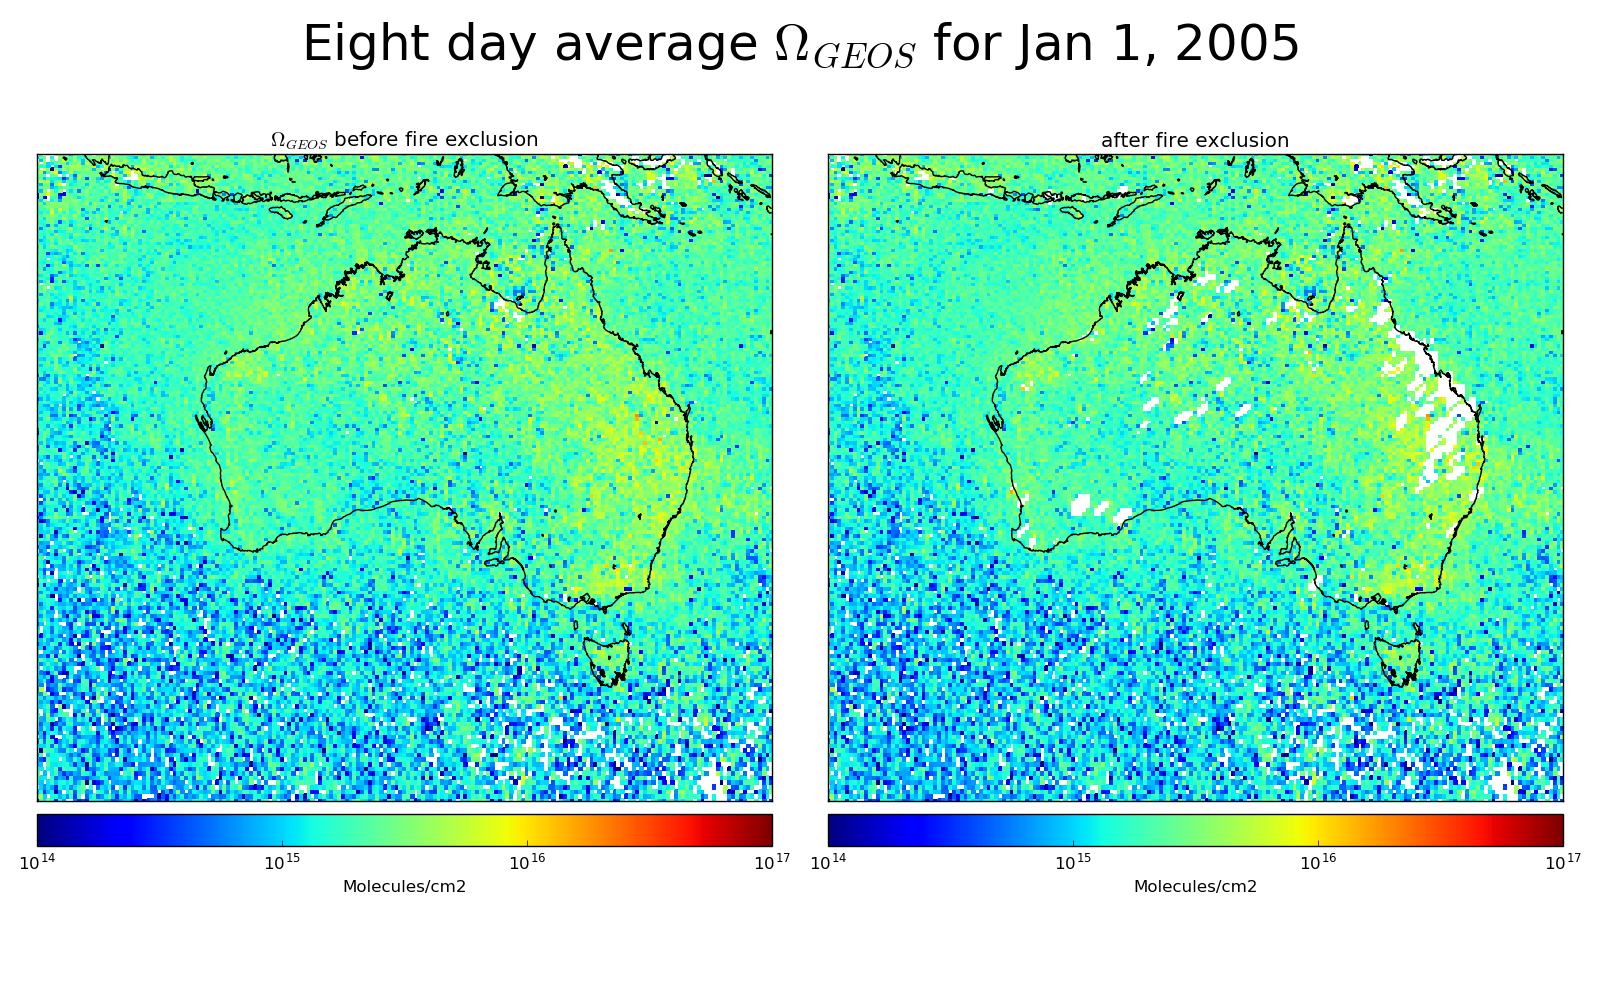
\includegraphics[width=\textwidth]{Figures/HCHO/fire_exclusion_aus_8d.png}
      \caption{Vertical column HCHO calculated using OMI satellite swaths with GEOS-Chem aprioris, averaged over 1-8 January 2005 with and without fire affected squares removed.}
      \label{ch_HCHO:fig:fireexclusionexample}
    \end{center}\end{figure}
    
    This filtering ends up removing too much information, and the recalculation of HCHO is too negatively influenced.
    To deal with this a separate product from the same instrument has been downloaded: MYD14A1, which keeps daily fire counts.
    Less disruptive filtering can be achieved by removing pixels which coincide with fires on the same day, as shown in figure TODO: which compares the 8 and 1 day filtering.
    TODO: The script to read and regrid these one day fire counts was adapted from X.
    Figure (TODO: effect on uncertainty and time series of fire pixels removed) shows the daily filtering effect on uncertainty and time series of fire pixels removed.
    
  \subsection{Filtering anthropogenic HCHO}
    TODO
  
  \subsection{Recalculating the AMF to create our own vertical HCHO columns}
  \label{ch_HCHO:sec:recalculating_AMF_description}
    OMI's apriori shape factor is based on the GEOS-Chem (v9) model, which uses 47 layers between the earth's surface and the top of the atmosphere using a pressure-eta hybrid (the actual values are shown in table \ref{app_a:tab:gc_47_vgrid}).
    Taking a more recent GEOS-Chem apriori shape factor and integrating along the vertical axis using equation \ref{ch_HCHO:eqn:AMFintwSdz} gives us a new AMF (AMF$_n$).
    Since we are using the $\omega$ provided by OMI, we remove the AMF$_G$ term from this calculation.
    The integration is done in Python using a simple rectangular method, which multiplies the integrand midpoints by the change in height, and then takes the sum.
    This is identical to calculating the integral if we assume the integrand is linear between each measured point, and introduces no new uncertainty.
    All that remains for recalculating the total vertical column using our new apriori shape factor is to apply the new AMF and remove the old:
    \begin{equation*}
      \Omega_{new} = \Omega \frac{AMF}{AMF_n}
    \end{equation*}
    
    The vertical column scattering weights and apriori shape factors provided in the OMHCHO dataset are defined on 47 levels.
    In order to reformulate the vertical column using updated GEOS-Chem hcho apriori shape factors I have run GEOS-Chem version 10.01 on the full 72 level vertical grid at 2 by 2.5 (lat by lon) degree monthly resolution. 
    The simulated vertical profiles of HCHO are averaged from 1300-1400 local time in order to match the satellite overpass time of roughly 1330.
    These vertical profiles then provide the apriori shape factor for the higher horizontally resolved satellite columns, which pick the nearest apriori from the model.
    TODO: determine which of these is correct!
    a)The new apriori profiles are monthly averages, which is the same temporal resolution used by the OMI apriori shape factors.
    b)The new apriori profiles are simulated daily and averaged over 8 days along with the recalculated total vertical columns.
    
    A new AMF is determined using equation \ref{ch_HCHO:eqn:AMFintwSdz}) with the apriori shape factor set by our GEOS-Chem model run.
    In order to reformulate the AMF, GEOS-Chem's 72 level vertical profile is transformed from ppb to a normalized number density profile in order to match equation \ref{ch_HCHO:eqn:ShapeFactor}. 
    This conversion uses the following equation: 
    \begin{equation} \label{ch_HCHO:eqn:ppbto}
      \eta_{HCHO} = ppb_{HCHO} \times \eta_a \times 10^{-9}
    \end{equation}
    where $\eta_{HCHO}$ is the number density of a HCHO, and ppb$_{HCHO}$ is the molecules of that species per billion molecules of air.
    In order to normalize these vertical density profiles over the globe, we divide by the modelled total vertical column $\Omega_{HCHO}$ which is determined by:
    \begin{equation*}
      \Omega_{HCHO} = 2.12\times 10^{13} \Sigma_z \left( ppb_{HCHO}(z) (P(z)-P(z+1)) \right)
    \end{equation*}
    where P(z) is the pressure (hPa) at the bottom of altitude level z, the constant 2.12e13 is determined from equation (TODO: run through this number in another section?).
    In effect this equation sums over the molecules per cm$^2$ in each altitude level.
    
    We have S$_z(z)$ and $\omega(z)$ over the vertical pressure coordinate z at all latitude and longitude points on whatever grid we wish. 
    A conversion to the sigma ($\sigma$) vertical coordinate is performed using $ P = \sigma (P_S - P_T) + P_T$, where $P_T$ is pressure at the top of the atmosphere and $P_S$ is surface pressure.
    In the sigma coordinate system we calculated the shape factor as follows:
    \begin{equation} \label{ch_HCHO:eqn:ShapeFactorSigma}
      S_\sigma(\sigma) = \frac{\Omega_a}{\Omega_v}C_{HCHO}(\sigma)
    \end{equation}
    where $\Omega_a$ is the vertical column of air from the surface to the top of the atmosphere and C$_{HCHO}(\sigma)$ is the mixing ratio of HCHO.
    This equation comes from \citet{Palmer2001}, and is unitless since $\Omega_a / \Omega_v$ is molecules of air per molecule of HCHO; the opposite of $C_{HCHO}$.

    Pressure dimension from OMI are the surface pressures from each gridbox (offline conversation with Dr Christopher Miller).
    Determining the geometric pressure midpoints (here onwards pressure levels) and interpolating to our increased vertical resolution involves a few steps.
    The lowest level (with highest pressure) in whichever pressure dimension (ours or OMI's) extends to the lowest altitude (or highest pressure) is interpolated upwards to match the lowest level in the other dimension.
    Secondly, if the OMI dimension has been changed, the scattering weights are interpolated onto this updated dimension.
    Figure \ref{ch_HCHO:fig:AMF_Surface_Relevel} shows how these first two steps are applied using three fake array comparisons and updating the array with the lower surface level.
    Finally, once our dimensions match at the surface (we are not so worried about the very top of the atmosphere) we interpolate the scattering weights onto our updated GEOS-Chem pressure dimension.
    
    \begin{figure}[!htbp]
      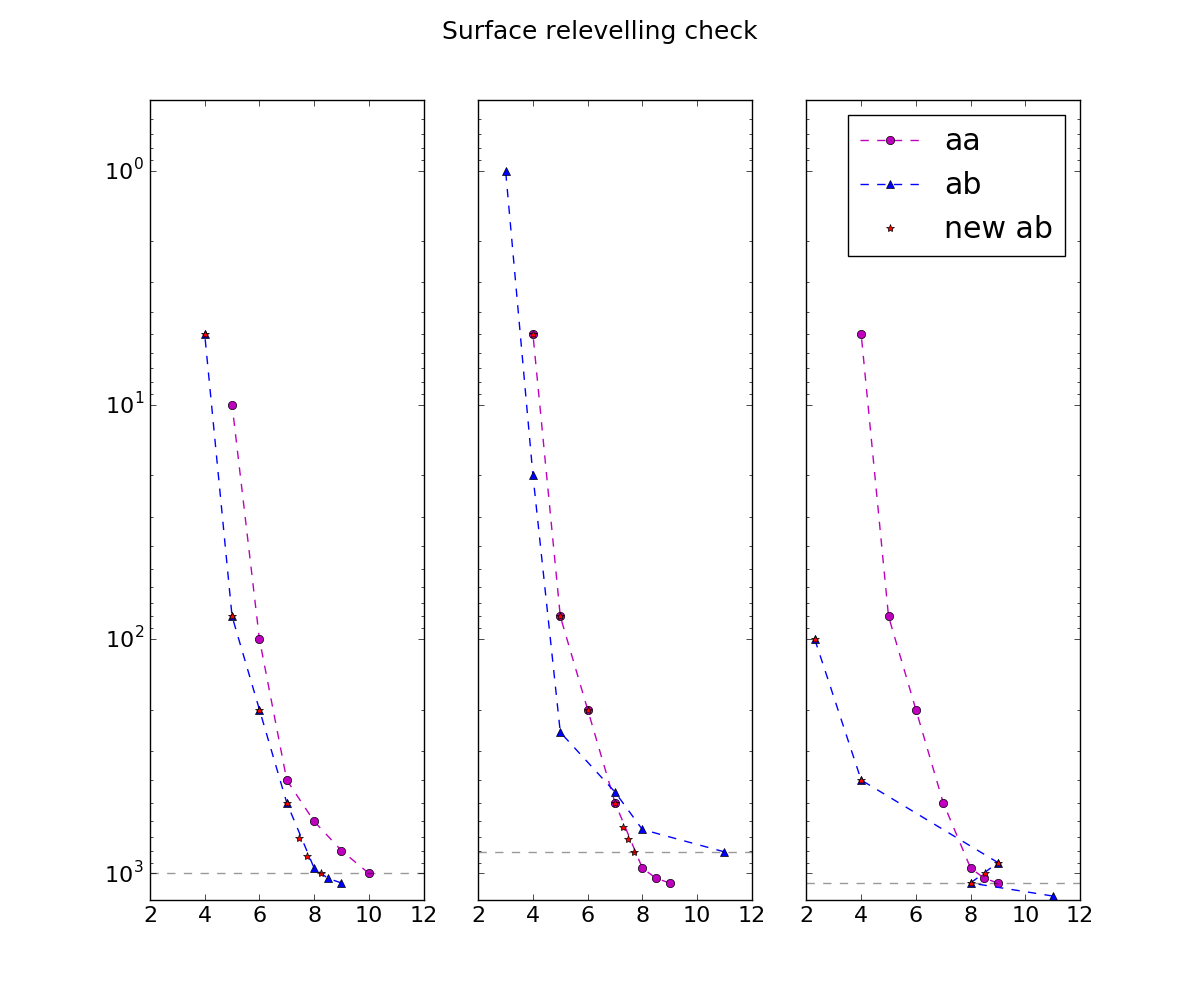
\includegraphics[width=\textwidth]{Figures/HCHO/SurfaceRelevelCheck.png}
      \caption{Constructed example of the initial interpolation of OMI's $\omega$ onto a pressure dimension with mismatched surface pressure.}
      \label{ch_HCHO:fig:AMF_Surface_Relevel}
    \end{figure}
    
    %If I change this to use an inverted geometric midpoint calculation then I need to explain it, otherwise I will need to note the assumption
    %$ \sqrt{ \left( P_1 \times P_{surf} \right)} = P_0 $
    %becomes $ P_{surf} = \frac{P_0^2}{P_1} $ where currently I'm using $P_0$ as the surface.

    S$_\sigma(\sigma)$ Is determined after running GEOS-Chem, which outputs vertical profiles of air density and HCHO mixing ratio, at 72 vertical levels with associated metadata such as vertical layer height and pressure, grid box location, height, and surface pressure.
    Using these outputs the vertical columns ($\Omega_a, \Omega_v$) are calculated for each horizontal grid point (i, j) as follows:
    \begin{align*}
      \Omega_a(i,j) &=& \Sigma_z \left( N_a(i,j,z) \times H(i,j,z) \right)
      \\
      \Omega_z(i,j) &=& \Sigma_z \left( N_{HCHO}(i,j,z) \times H(i,j,z) \right)
    \end{align*}
    where $N_a$, and $N_{HCHO}$ are the densities of air and HCHO, H is the layer height (for each grid box).
    Note that HCHO density is determined from the outputted mixing ratio: $N_{HCHO} = C_{HCHO} \times N_a$.

    S$_\sigma(\sigma)$ is then stored in HDF-EOS5 format, to be used in conjunction with the satellite measurements to calculate an AMF as shown in equation \ref{ch_HCHO:eqn:AMFintwSdz}.
    As the GEOS-Chem V10.01 output is in bitpunch format, the code to read the data and create the shape factor is written in IDL, which has many procedures and functions which are already written to handle reading this format (provided by GAMAP).
    The code is provided in supplementary TODO: put code into supplement section.
    
    For each OMI slant column, a new AMF is calculated using S$_\sigma(\sigma)$ and the provided scattering weights $\omega(\sigma)$ using equation \ref{ch_HCHO:eqn:AMFintwSdz}.
    This integral is applied in python by taking the sum of S$_\sigma(\sigma) \times \omega(\sigma) \times \mathrm{d}\sigma$ for each $\sigma$ determined at 72 levels in GEOS-Chem, with the provided $\omega$ interpolated linearly to these same levels.
    An example of these interpolations is shown in figure TODO: interpolation figure with symbols at original points and interpolated line overplotted for both functions over hPa.
    Globally this reprocessing changed the AMF by TODO: global total percent difference in AMF. 
    In total this caused TODO: total column HCHO change globally/yearly
    In Summer over Australia the global AMF difference was TODO: Difference summers only.
    This changed Australia's HCHO amounts from TODO: X to Y Tg per year plus minus one std.
    
  \subsection{AMF code from Paul Palmer}
  \label{ch_HCHO:sec:PPCode}
    TODO: describe how I use this here
    I use code originally written by Dr. Paul Palmer with various updates and modifications described in section (TODO:) as another way to recalculate the AMF using information from the satellite swaths and the GEOS-Chem overpass simulation output.
    These are used to recalculate the instrument sensitivity or scattering weights for each pixel, as well as the shape factor which together are integrated to give the pixel AMF.
   
   GEOS-Chem outputs quantities averaged between 1200 and 1400 LT, including optical depths at several wavelengths (TODO: list), dust, and HCHO.
   I run a script on the satellite swaths which pulls out a subset of the pixel information into a daily csv file, which can be read by the AMF code as modified by Dr. Luke Surl, in conjunction with the GEOS-Chem outputs for each day.
   The AMF code is then run and produces a csv of recalculated AMFs which get read by my python code and associated with the corresponding pixel.
    
  \subsection{Determination and application of the pacific ocean reference sector normalisation}
    \label{ch_HCHO:sec:RSC}

    As is done in \citet{Abad2015}, a reference sector defined over the Pacific ocean is used to correct OMI instrument degradation.
    This correction is calculated based on satellite measurements over the pacific ocean reference sector; between 140$^{\circ}$W and 160$^{\circ}$W, covering every latitude.
    Corrections are made using apriori HCHO columns in the same reference sector modelled using GEOS-Chem.
    The apriori reference sector of HCHO vertical columns (VCs) is created by GEOS-Chem using 15 minute time resolution, with 2 by 2.5$^{\circ}$ latitude by longitude resolution.
    These simulated values use the GEOS-Chem output averaged between 1300 and 1400 local time at each grid box, in order to match the overpass time of OMI.
    The longitudinal average is taken within the apriori reference sector, as corrections are assumed to be longitudinally invariant.
    The modeled reference sector is interpolated latitudinally in for use in the OMI measurement correction array creation.
    Figure \ref{ch_HCHO:fig:Summary_RSC} the simulated reference sector VCs as an example, calculated on January 1st 2005.
    In this figure the vertical resolution is increased from 2$^{\circ}$ to 0.36$^{\circ}$, through linear interpolation, in order to form 500 vertical bins which are used in correcting the satellite data.
    Each day, good satellite measurements taken over the reference sector are used to determine a correction array.
    The correction is based on the difference between measured slant column and the modeled slant column within the reference sector.
    The model does not produce slant columns associated with each measurement, however one is created by multiplying the VC with the associated slant column's AMF.
    
    \begin{figure}[!htbp]\begin{center}
      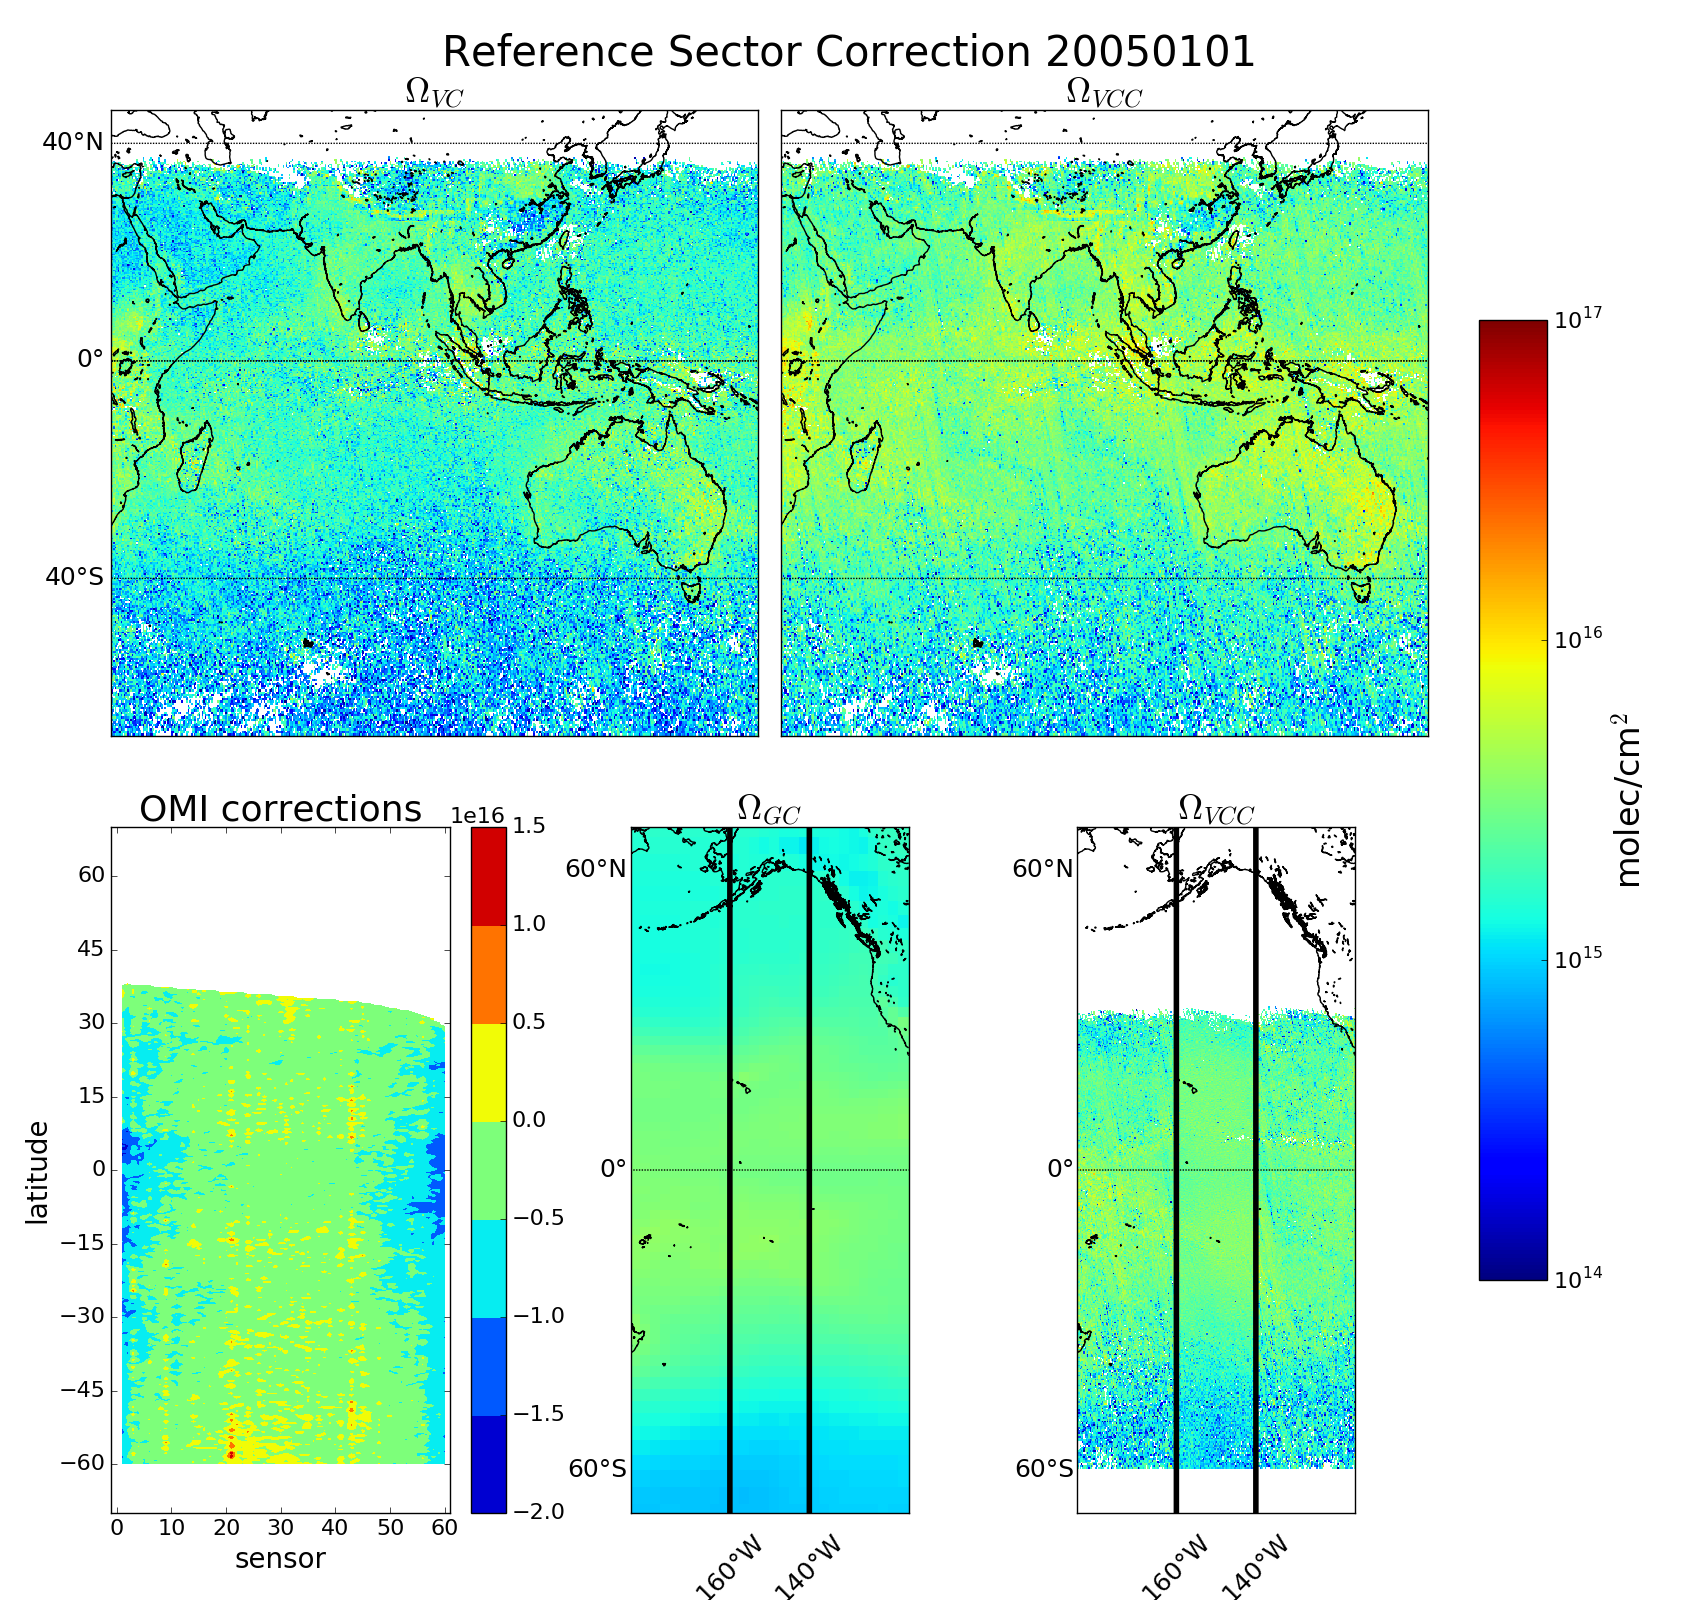
\includegraphics[width=0.7\textwidth]{Figures/HCHO/Summary_RSC_Effect8d_20050101.png}
      \caption{ %
	Example of remote pacific reference sector correction (RSC) using 8-day average measurements and one month modelled data.
	$\Omega_{VC}$ shows the uncorrected vertical columns, while $\Omega_{VCC}$ shows the corrected vertical columns.
	OMI corrections shows the correction applied globally based on latitude and OMI track number(sensor).
	$\Omega_{GC}$ shows the GEOS-Chem modelled HCHO VC over the RSC, with $\Omega_{VCC}$ showing the corrected VC over the same area.
      }
      \label{ch_HCHO:fig:Summary_RSC}
    \end{center}\end{figure}
    
    For OMI swaths, each row of measured data contains 60 `Across track'(track) measurements.
    The track index (i) relates a the measurement to one of the 60 columns of data.
    Corrections for each measurement are calculated by taking the difference between the measured slant column and the apriori slant column as follows:
    \begin{equation} \label{ch_HCHO:eqn:reference_sector_correction}
      Correction(i,j) = SC_{HCHO}(i,j) - VC_{GEOS-Chem}(lat(j)) \times {AMF_{OMI}}(i,j)
    \end{equation}
    where j represents a latitude index and $VC_{GEOS-Chem}(lat)$ represents the apriori reference sector vertical column HCHO at the latitude corresponding to j.
    Note that the correction is in molecules per cm$^2$.
    
    The reference sector correction is independently calculated for each of the 60 tracks, at each latitude where a good satellite measurement exists which used that track.
    The Correction$(i,lat(j))$ function is determined by binning corrections for each track into 500 equidistant latitude bands. 
    
    Due incomplete latitudinal coverage, the correction for each track is interpolated linearly between measurements, with corrections outside of the highest measured latitudes being equal to the corrections at the highest measured latitudes.
    Figure \ref{ch_HCHO:fig:track_correction_interpolations} shows an example of the 60 track corrections for January 1st 2005, the points are satellite measurements and the lines are the interpolations for each track.
    \begin{figure}[!htbp]\begin{center}
      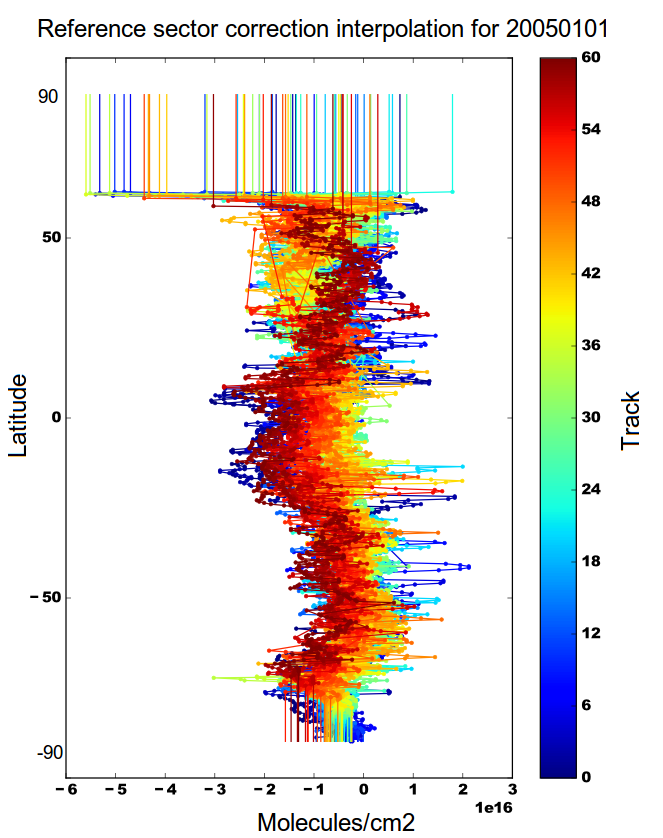
\includegraphics[width=0.7\textwidth]{Figures/HCHO/track_corrections20050101.png}
      \caption{Example of track correction interpolations for January 1st 2005, points represent satellite slant column measurements, with lines interpolating and extrapolating along the latitudinal direction.}
      \label{ch_HCHO:fig:track_correction_interpolations}
    \end{center}\end{figure}
    
    Another way to look at this correction is given in the OMI corrections panel of figure \ref{ch_HCHO:fig:Summary_RSC}, which has the sensors along the x axis, and latitude on the y axis, and shows how for this example 8-day period, the corrections are distributed with more negative values towards the left or right sensors, especially in the tropics.
    
    One correction is associated with every good satellite measurement which is used to create a reference sector corrected measurement (Vertical Column Corrected or VCC) through the following equation:
    \begin{equation}
      VCC(i,j) = \frac{SC_{HCHO}(i,j) - Correction(i,lat(j))}{AMF(i,j)}
    \end{equation}
    Finally, for each day, the good satellite measurements are averaged into our own latitude longitude resolution bins along with the associated corrected SC, VC, VCC, AMF, and bin entry count.
    The bin entry count is used to create an 8-day average out of the one day averages, as it is the daily mean multiplied by the daily count summed over 8 days divided by the total count for each bin.
    
  \subsection{Estimation of error or uncertainty}
  \label{ch_HCHO:sec:OMI_uncertainty_calculation}
    There are three main sources of error in the resulting HCHO columns:
    \begin{description}
      \item[a] Fitting error from the OMI retrieval.
      \item[b] Uncertainty in AMF calculations.
      \item[c] Uncertainty of HCHO background.
    \end{description}

    a) is available in the OMI product and reduced through spatial and temporal averaging.
    Taking the eight day grided average with horizontal resolution of 0.25 by 0.3125 degrees (latitude by longitude) typically reduces uncertainty by a factor of 1.5 to 4.
    Another method for examining uncertainty of OMI is to analyse the standard deviation of the HCHO columns over the remote pacific.
    If we assume there is no HCHO variation from background levels over any 8-day period, then this method infers variations in the measuring instrument, and can be used as a metric for uncertainty as done in \citet{DeSmedt2012}.
    TODO: uncertainty calculation on remote pacific OMI.
    \cite{Millet2006, Palmer2006} both examine OMI HCHO columns over North America and determine overall uncertainty to be 40\%, with most of this coming from cloud interference.

    b) is determined through an analysis of GEOS-Chem output, validated against the total column of HCHO at Wollongong using FTIR measurements from the (TODO: Nicholas Jones roof HCHO citation here).
    \cite{Palmer2006} calculate the error in AMF through combining estimates of error in the UV albedo database ($\sim 8$\%), model error based on in-situ measurements, cloud error  ($20-30$\%) \citep{Martin2003}, and aerosol errors ($<20$\%), totalling AMF error of around $\sim 30$\%.
    It is worth noting here that independent error estimates are added in quadrature, which means total error equals the root of the sum of the independent errors each sqaured ($e_{Total}=\sqrt{\Sigma_i e_i^2}$).
    TODO:Paul palmer calculation and combination for overall Satellite VC uncertainty per pixel and gridded.
    TODO: Millet2008?
    
    c) is also determined through a study of GEOS-Chem output, in relation to in-situ measurements.
    TODO: calculate this uncertainty.
    Compare this error estimate with that of \citet{Curci2010}, where the error in b) and c) are respectively found to be 30\% and 15\% based on their analysis of CHIMERE.
    \cite{Millet2008} also examine this uncertainty and determine an overall uncertainty ($1\sigma$) of $25-27%$ in HCHO vertical columns with calculated AMFs where cloud fraction $< 0.2$.
  
\section{Validation and comparisons}
  \label{ch_HCHO:sec:Validation}
  
  \subsection{Comparison with standard OMI product}
    Figure TODO: shows global and Australian HCHO eight day averaged total column maps for 1-8 January 2005, along with the reduced major axis (RMA) regression corellation and percentage difference.
   This comparison shows how reprocessing with an updated model can have a systematic influence on the total column.
  
  \subsection{Comparison with in-situ measurements}
    TODO: Describe Wollongong FTIR and junk
    Analyse comparison of gridbox with instrument!

  \subsection{Summary}
    First the OMI HCHO level 2 data was downloaded, and read using python creating a list of good pixels for each day.
    Next the associated AMF and reference sector correction for each good pixel was calculated using GEOS-Chem for the apriori shape factor, and using the provided scattering weights from OMI.
    Each 8 days the pixel list is averaged onto a 0.25$^{\circ}$ latitude by 0.3125$^{\circ}$ longitude grid.
    The new HCHO product along with counts and average uncertainty of pixels used in the grid square is also kept.
    The product includes the 8-day gridded averages of the old and new AMFs, the average correction sector from GEOS-Chem over the pacific ocean, and the old and new HCHO with and without the reference sector correction from \cite{Abad2015} applied.
    
    \subsection{Conclusions}

    % CHAPTER 3 (probably)
% Isoprene Emissions

\chapter{Isoprene Emissions in Australia} % Main chapter title
\label{ch_isop}

\section{GEOS-Chem isoprene mechanisms}
\label{ch_isop:sec:GEOSChemMechanisms}
  \subsection{Outline}
    The isoprene reactions simulated by GEOS-Chem were originally based on \cite{Horowitz1998}.
    This involved simulating NO$_X$, O$_3$, and NMHC chemistry in the troposphere at continental scale in three dimensions, with detailed NMHC chemistry with isoprene reactions and products.
    The mechanism was subsequently updated by \citet{Mao2013}, who change the isoprene nitrates yields and add products based on current understanding as laid out in \citet{Paulot2009a,Paulot2009b}.
    Further mechanistic properties, like isomerisation rates, are based citet{Crounse2011,Crounse2012,Peeters2010,Peeters2011}.
    (TODO: check abstracts of these papers)
    \cite{Crounse2011} examines the isomerisations associated with the oxidation of isoprene to six different isomers (ISO$_2$) formed in the presence of oxygen: isoprene $ + OH \rightarrow^{O_2} $ ISO$_2$.
    They determine rates and uncertainties involved in these reactions.
    \cite{Crounse2012} examine the fate of methacrolein (MACR), one of the products of isoprene oxidation. 
    Prior to this work MACR oxidation chamber studies were performed in high NO or HO$_2$ concentrations, giving peroxy lifetimes of less than 0.1~s.
    In most environments this is not the case, and MACR products over various NO concentrations and peroxy radical lifetimes are determined in their work.
    
    Formation of isoprene nitrates have an effect on ozone levels through NO$_X$ sequestration, and the yields and destinies of these nitrates is analysed in \citet{Paulot2009a}. 
    They use anion chemical ionization mass spectrometry (CIMS) to determine products of isoprene photooxidation.
    In a chamber with clean air and high NO concentrations, isoprene photooxidation is initially driven by OH addition, followed by NO$_X$ chemistry (150~min - 600~min), and finally HO$_X$ dominated chemistry.
    The yields of various positional isomers of isoprene nitrates is estimated, and pathways of their oxidation products is shown and used in the GEOS-Chem isoprene mechanism \citep{Paulot2009a,Mao2013}. 
    
    In low NO$_X$ conditions, isoprene oxidises to yield 70\% hydroxyhydroperoxides (ISOPOOH), which then oxidises to create dihydroxyperoxides (IEPOX) with OH recycling maintaining the OH levels in the atmosphere \citep{Paulot2009b}.
    In older models isoprene produced ISOPOOH which then titrated OH, however, the loss of OH has not been seen in measurements \citep{Paulot2009b,Mao2013}.
    The isoprene mechanism in GEOS-Chem has been updated to include OH regeneration from oxidation of epoxydiols and slow isomerisation of ISOPO$_2$ \citep{Mao2013}.
    
    Under high NO$_X$ conditions, isoprene undergoes OH addition at the 1 and 4 positions, becoming $\beta$ (71\%) or $\delta$ (29\%) hydroxyl peroxy radicals (ISOPO$_2$). 
    The $\beta$-hydroxyl reacts with NO$_X$ and produces HCHO (66\%), methylvinylketone (40\%) (MVK), methacrolein (26\%), and $\beta$-hydroxyl nitrates (6.7\%) (ISOPNB).
    The $\delta$-hydroxyl reacts with NO to form $\delta$-hydroxyl nitrates (24\%) (ISOPND), and ISOPNB (6.7\%).
    ISOPNB and ISOPND yield first generation isoprene at 4.7\% and 7\% respectively.
    
    Under low NO$_X$ conditions, ISOPO$_2$ may react with HO$_2$ to form ISOPOOH.
    In this case there is also production of HCHO (4.7\%), MVK(7.3\%), and MACR (12\%).
    As stated in earlier; most ISOPOOH will form IEPOX (epoxydiols) after reacting with OH and lead to OH regeneration.
    The other mechanism in low NO$_X$ environments is unimolecular isomerisation of ISOPO$_2$.
    This leads to production of hydroperoxyaldehydes (HPALDS), which generally photolyse and have an OH yield of 100\%.
    \citet{Mao2013} show that a lower (factor of 50) rate constant for ISOPO$_2$ isomerisation leads to better organic nitrate aggreements with ICARTT. 
    
    This update leads to more accurate modelling of OH concentrations, especially in low NO$_X$ conditions common in remote forests.
    Prior to \citet{Mao2012}, measurements of OH in high VOC regions may have been up to double the real atmospheric OH levels, due to formation of OH inside the instrument.
    \citet{Mao2012} examine an upgraded method of measurement, and compare these against a regional atmospheric chemistry model (RACM2), with the OH recycling updates from \citet{Paulot2009b} as discussed in prior paragraphs.
    
    The updates to isoprene chemistry by \citet{Mao2013}, and those shown in \cite{Crounse2011,Crounse2012} are the last before version 11, which was not used in this work.

    The full current mechanism is described online at \url{http://wiki.seas.harvard.edu/geos-chem/index.php/New_isoprene_scheme}.
    
  \subsection{Emissions from MEGAN}
    MEGAN simulates biogenic emissions of various gases including isoprene, based on various meteorological, land cover, and plant type parameterisations.
    
    One of the important parameters in Australia is the soil moisture activity factor($\gamma_{SM}$), which can have large regional affects on the isoprene emissions \citep{Sindelarova2014,Bauwens2016}.
    Generally if soil moisture is too low, isoprene emissions stop \citep{Pegoraro2004,Niinemets2010}, however in many Australian regions the plants may be more adapted to lower moisture levels. (TODO: Find cites for this - talk from K Emerson at Stanley indicated this)
    GEOS-Chem runs MEGANv2.1, which has three possible states for isoprene emissions based on the soil moisture ($\theta$):
    \begin{align*}
      \gamma_\mathrm{SM} & = 1 && \theta > \theta_1 \\
      \gamma_\mathrm{SM} & = (\theta-\theta_w)/\Delta\theta_1  && \theta_w < \theta < \theta_1 \\
      \gamma_\mathrm{SM} & = 0 && \theta < \theta_w \\
    \end{align*}
    where $\theta_w$ is the wilting point, and $\theta_1$ determines when plants are near the wilting point.
    The wilting point is set by a land based database from \citet{Chen2001}, while $\theta_1$ is set globally based on \citet{Pegoraro2004}. (TODO: Check Chen2001 from Guenther2006)
    
    In GEOS-Chem the emissionscan be globally multiplied by a constant factor, which was performed to determine the smearing and sensitivity.
    By running the model two extra times, with the biogenic emissions set to zero and one half, while other parameters remain unchanged, the general affects of isoprene emissions which the model undergoes can be determined.
    
%----------------------------------------------------------------------------------------
%	SECTION
%----------------------------------------------------------------------------------------
\section{Isoprene emissions estimation}
\label{ch_isop:sec:IsopreneEmissions}

  \subsection{Outline}
   With the vertical columns of biogenic HCHO we can infer the local (grid space) isoprene emissions using effective molar formaldehyde yield (In other continents around 2-3, or 1 in low NO$_X$ conditions) \citep{Palmer2003,Marais2012,Bauwens2016}.
    If we assume there is fast HCHO yield, so that the effect of chemical transport is minimal, and that HCHO and isoprene are at steady states, then we can calculate local yield from our CTM.
    %This yield is derived from both HCHO and isoprene, such as was used by \citet{Millet2006} who produced a molar HCHO yield of 2.3 in north eastern USA.
   Yield is calculated from the modelled slope between isoprene emissions and HCHO total column within each gridbox over Australia, as performed in \cite{Palmer2003}, using modelled values between 1300-1400 LT which is around the overpass time of the OMI.
   This modelled yield is then used in conjunction with the recalculated OMI measurements in order to estimate isoprene emissions.
    
    The calculations used to determine isoprene emissions over Australia are fully described in \ref{ch_isop:sec:EmissionCalculation} and follow the method of \citet{Palmer2003}.
    To calculate emissions we use a reduced major axis (RMA) regression between modelled average (from 1300-1400 LT) values of the loss rates and total columns, an example is shown in figure TODO: figure with RMA of these over whatever time and space I end up using.
    
    The measured background HCHO is the average concentration measured in the remote pacific at the same time.
    The modelled background is determined from a run with isoprene emissions turned off, which allows us to see exactly how much the modelled isoprene emissions alter each vertical column of HCHO.
    
    Isoprene quickly forms HCHO in the atmosphere when in the presence of high levels of NO$_X$.
    However, over Australia NO$_X$ levels are generally not high enough and we must take extra care that we can account for the transport or 'smearing' caused by slower HCHO formation.
    Smearing sensitive grid boxes within the model can be detected by running the model with two uniformly differing isoprene emission levels, then finding the grid boxes where the changed HCHO column is greater than can be attributed to local emission difference.
    Using equation \ref{ch_isop:eqn:isop_yield} with two different isoprene emission levels:
    \begin{equation*}
      \hat{S} = \frac{\Delta~\Omega_{HCHO}}{\Delta~E_{ISOP}}
    \end{equation*}
    Consider halving the isoprene emitted globally and rerunning the model, if the local grid HCHO is reduced by much more than half (factoring yield) then you can infer sensitivity to non-local isoprene emissions.
    This can be dependent on local or regional weather patterns, as greater wind speeds will reduce the time any emitted compound stays within the local grid box.
    As such smearing sensitivity is both spatially and temporally diverse, shown in figure TODO: is a picture of the smearing sensitivity over Australia.
   
    Once the smearing sensitive grid squares are filtered out, application of equation \ref{ch_isop:eqn:isop_yield} gives us an estimate of isoprene emissions across the nation.
    
    Most recently a \citet{Bauwens2016} undertook a similar process to what I am doing, although with slightly different focus, using the IMAGESv2 global CTM instead of GEOS-Chem.
    They calculate emissions which create the closest match between model and satellite vertical columns, and compare these postiori data with the apriori (satellite data) and independent data sets.
    (TODO: simple outline of what they did and how my focus is different, this paper will also need to be summarised in the LitReview)

  \subsection{HCHO Products and yield}
    Australian forests are strong emitters of both isoprene and monoterpenes, which go on to form various products including but not limited to secondary organic aerosols, oxygenated VOCs (OVOCs), ozone, OH, and HO$_2$.
    This production occurs over several steps, yields are often classed into at least two categories.
    First generation yield refers to the amount of HCHO produced per unit isoprene consumed by initial oxidation, total yield (sometimes molar yield) refers to time dependent yield of HCHO over multiple oxidation stages \citep{Wolfe2016}.
    \citet{Wolfe2016} define prompt yield as the change in formaldehyde measurement per unit change in initial isoprene emissions.
    Some argue that isoprene emissions are overestimated, due to the fact that they are based on relatively few measurements of isoprene emission factors \citep{Winters2009, FortemsCheiney2012} TODO: read and cite paper mentioned in Fortems.
    
    Isoprene production of HCHO depends on several factors, importantly NO$_X$ levels have a direct effect on the fate of VOCs in the atmosphere.
    At higher NO mixing ratios (at least a few hundred pptv), organic peroxy radicals (RO$_2$) react mostly with NO. 
    At low NO (less than 10's of pptv), reaction with HO$_2$, other RO$_2$, and isomerization dominate the fate of RO$_2$.
    In low NO$_X$ environments, reported HCHO yields from isoprene are from XtoY\%, while in high NO$_X$ environments this value is XtoY\% TODO: these values from table.
    For monoterpenes the yields are around X, Y\% for low, high NO$_X$ respectively.
    Emissions and yields for various species including some terpenes can be seen in table \ref{ch_isop:tab:VOCAusYields}.
    \citet{Wolfe2016} determine that going from NO$_X = 0.1$ to $2.0$ ppbv triples the prompt yield of HCHO, from 0.3 to 0.9 ppbv ppbv$^{-1}$ due to isoprene, while the background HCHO doubles.
    They determine prompt yield as the change in HCHO per change in ISOP$_0$, using $[ISOP]_0=[ISOP]\exp(k_1[\mathrm{OH}]t)$; where $k_1$ is first order loss rate.
    This effectively relates HCHO abundance with isoprene emission strength.
    (TODO:and finish Wolfe2016 discussion paper for yields)
    TODO:go through atkinsonarey2003
    
    Many of the HCHO yields from terpenoids are estimated through chamber studies which examine the products molecular mass and charge after mixing the compound of choice into a known volume of air.
    These conditions generally don't match those of the real world, where ambient air will have a cocktail of these compounds as well as various reactants.
    
    A proton transfer reaction mass spectrometer (PTR-MS) can be used to determine gas phase evolution of terpene oxidation products.
    This is done through analysis of mass to charge ratios ($m/z$) which can be used identify chemical compounds.
    Looking at Australian emissions from running GEOS-Chem and using yields provided by XYZ (TODO other table), we see that Australia may be more or less likely to do something TODO: this comparison sentence would be good to tie up tables and be copied to conclusions.
    
    Conversions between HCHO per unit C yield and molar \% yield from species X given by the equation $ Y_{molar \%} = 100 \times C_X \times Y_{HCHO per unit C} $, where $C_X$ is how many Carbon are within species X (5 for isoprene, 10 for monoterpenes, etc...).
    For instance a 200\% molar yield of HCHO from isoprene implies 1 Mole of C$_5$H$_8$ becomes 2 Mole HCHO which is a 0.4 HCHO per unit C yield.
    
    TODO: Fill out this table
    \begin{table} \begin{threeparttable}
      \caption{HCHO yields from various species averaged over Australia during Summer.}
      \begin{tabular}{ | c  c  c  c  c | }
        \toprule
	  \textbf{Species}   & \textbf{Emissions$^a$}& \textbf{Lifetime$^b$}& \textbf{HCHO Yield$^c$} & \textbf{HCHO production$^d$\%}
	  \\                 & (Tg C per month)      &                      & (per C reacted)         &         \\
	\midrule
	  Isoprene           & Y                     & n minutes            & 0.x                     & 10       \\
	  $\alpha$-Pinene    & Y                     & n minutes            & 0.x                     & 10       \\
	  $\beta$-Pinene     & Y                     & n minutes            & 0.x                     & 10       \\
	  HCHO               & Y                     & n minutes            & 1.0                     & 10       \\
	\bottomrule
      \end{tabular}
      \begin{tablenotes} 
	  \item a: Calculated using GEOS-Chem emissions over Australia in January 2005.
	  \item b:  
	  \item c: 
	  \item d: Production determined by dividing emission*yield by the sum of all VOC emissions*yields. 
      \end{tablenotes}
      \label{ch_isop:tab:VOCAusYields}
    \end{threeparttable} \end{table}
    
    % yields from Atkinsen2003
    %isoprene
    %0.63 0.10 Tuazon and Atkinson (1990a)
    %0.57 0.06 Miyoshi et al. (1994)
    % a-pinene
    %0.23 0.09 Noziere et al. (1999a)
    %0.19 0.05 Orlando et al. (2000)
    % b-pinene
    %0.54 0.05 Hatakeyama et al. (1991)
    %0.45 0.08 Orlando et al. (2000)
    
    Yields table looking at literature provided yields of HCHO.
    % molar HCHO yield per unit carbon equal to HCHO molar percent yield(per carbon)? or some conversion?
    % TODO: ask steve about ppbv ppbv^-1 ??
    
    \begin{table} \begin{threeparttable}
      \caption{ HCHO yields from various species, and lifetime against oxidation by OH. }
      \begin{tabular}{  l  l  l  l  l  }
      	\toprule
      	Species    & HCHO Yield      & Life vs OH & NO$_X$ background & Source	\\
                      & (molar \% )        &               &                          &          \\
      	\midrule 
      	Isoprene	& 315$\pm$50      &              & High           & a        \\ 
      			& 285$\pm$30      &        & High               & a        \\ 
      			& 225             & 35 min & High               & b        \\ % Done
      			& 150             &            & Low                & b        \\ % Done
      			& 150             &            & Low                & d        \\
      			& 450             &            & High               & d        \\
			& 235             &            & 1~ppbv              & e        \\
			& 150             &            & 0.1~ppbv              & e        \\
	$\alpha$-Pinene & 28$\pm$3        &        & Low                & c        \\ 
			& X$\pm$3         &        & X                  & d        \\ 
      			& 230$\pm$90      &        & High        & a        \\ 
      			& 190$\pm$50      &        & High        & a        \\ 
      			& 19                & 1 hour &              & b        \\ % Done
                      & 210               &          & 1~ppbv              & e        \\
                      & 70                &          & 0.1~ppbv              & e        \\
	$\beta$-Pinene    & 65$\pm$6        &        & Low                & c      \\ 
      			          & X$\pm$3         &        & X                  & d      \\ 
      			          & 540$\pm$50      &        & High               & a     \\ 
      			          & 450$\pm$80      &        & High               & a      \\ 
      			          & 45              & 40 min &              & b      \\ % Done
	Methane 	      & 100             & 1 year  &             & b     \\ 
	Ethane            & 180             & 10 days &             & b     \\ 
	Propane           & 60              & 2 days  &             & b     \\ 
	Methylbutanol    & .13(per C)    & 1 hour  &             & b     \\ 
	HCHO             & 100             & 2 hour  &             & b     \\ 
	Acetone           & .67(per C)      & 10 days &             & b     \\ 
	Methanol          & 100             & 2 days  &             & b     \\ %Done
    	\bottomrule
    \end{tabular}
    \begin{tablenotes} % \item makes new lines
      \item a \citet{AtkinsonArey2003}: Table 2, Yield from Isoprene reaction with OH, two values are from two referenced papers therein.
      \item b \citet{Palmer2003}: lifetimes assume [OH] is 1e15 mol cm$^{-3}$.
      \item c \citep{Lee2006}: Calculated through change in concentration of parent and product linear least squares regression.
        Estimates assume 20$^\circ$~C conditions.
  	  \item d \citet{Wolfe2016}: ``prompt yield'': change in HCHO per change in ISOP$_0$.
  	    $[ISOP]_0=[ISOP]\exp(k_1[\mathrm{OH}]t)$; where $k_1$ is first order loss rate.
  	    Effectively relates HCHO abundance with isoprene emission strength
      \item e \citet{Dufour2009}: One-day yields from oxidation modelled by CHIMERE, using MCM reference scheme.
      \item f Calculated using PTR-MS and iWAS on SENEX campaign data.
    \end{tablenotes}
    \label{ch_isop:tab:VOCLiteratureYields}
  \end{threeparttable} \end{table}
    
  \subsection{CAABA/MECCA yield}
  \label{Ch_isop:sec:CAABAMECCA}
    CAABA/MECCA is described in \ref{ch_LitRev:sec:CAABAMECCAIntro}.
    
    Using CAABA/MECCA to examine isoprene to HCHO yield in specific scenarios allows us to determine what environment may be driving the yield calculated by GEOS-Chem.
    This software runs gas and aqueous phase, and heterogeneous chemistry, including basic HO$_X$, NO$_X$, and NMHC chemistry, with emission, deposition, and initial concentrations all set.
    By running the same simulation twice, and injecting a small amount of extra isoprene into one of the simulations, extra HCHO produced can be used to determine the yield from isoprene to HCHO.
    Isoprene life time can also be calculated using this process, as the time it takes for the extra isoprene to reach $1/e$ of it's initial value.
    
    Initially we have three scenarios, grassland, desert, and forest Australia - with each scenario having initial conditions, emission and deposition set as in table \ref{ch_isop:tab:CaabaMeccaScenarioYields}.
    Running each scenario with and without a small isoprene injection gives isoprene lifetimes and isoprene to HCHO yield for those scenarios, shown in table \ref{ch_isop:tab:CaabaMeccaScenarioYields}.
    Calculation of the yield follows a calculation of the theoretical maximum carbon production by the amount of injected isoprene:
    \begin{equation}
      Y_{100} =10^9 \times \frac{C_{PM} E_{inj} D_{inj}}{(N_A H_{PBL})}
    \end{equation}
    Where Y$_{100}$ is the maximum possible carbon yield of isoprene (ppb), $C_{PM}$ is Carbon per molecule (isoprene=5), $E_{inj}$ is the emission rate of injected isoprene (molec cm$^{-2}$ s$^{-1}$), $D_{inj}$ is the duration of injection (s), H$_{PBL}$ is the boundary layer height (cm), and $N_A$ is the Air number density (molec cm$^{-3} \approx 2.5e19$).
    Finding the accumulated increase in HCHO (ppb) from the difference between the perturbed and non perturbed model runs allows calculation of the accumulated extra HCHO (Example: Figure TODO:), which divided by the $Y_{100}$ gives us the isoprene to HCHO atom C yield:
    \begin{equation}
      Y_{HCHO}= \frac{\Delta HCHO_{\text{Accumulated}}}{Y_{100}}
    \end{equation}
    with $HCHO_{\text{Accumulated}}$ being the accumulated enhanced ppb mixing ratio of HCHO.
    
    TODO: Fill in table
    \begin{table}
    	\caption{Scenario isoprene yields of HCHO}
    	\begin{tabular}{ p{6cm} l  l  l  l }
    		\hline
    		\textbf{Scenario} & \textbf{Emission} & \textbf{NO$_X$} & \textbf{HO} & Yield \\
				    		  & (molecules units) & (units)         & (units)     & units \\ \hline
    		Forest 	& xx 	& xx 	& xx 	& xx  	\\ 
    		Urban 	& xx 	& xx 	& xx 	& xx 	\\
    		Shrub 	& xx 	& xx 	& xx 	& xx 	\\ \hline
    	\end{tabular}
    	\label{ch_isop:tab:CaabaMeccaScenarioYields}
    \end{table}
    
    Figure TODO: shows the accumulated yield for all three scenarios, which each increase towards a limiting value.
    
  \subsection{Calculation of Emissions}
    \label{ch_isop:sec:EmissionCalculation}
    As is done in \citet{Palmer2003, Millet2006, Bauwens2016}, we assume that HCHO, and Isoprene columns are in a steady state, with no horizontal transport.
    In these circumstances the emissions of precursors are easy to calculate as long as we know the molar HCHO yields (Y$_i$) and effective chemical loss rates (k$_i$):
    \begin{equation}
      \Omega_{HCHO} = \frac{1}{k_{HCHO}}\Sigma_i k_i Y_i \Omega_i = \frac{1}{k_{HCHO}}\Sigma_i Y_i E_i
    \end{equation}
    
    We can infer the local (grid space) isoprene emissions (E$_{isop}$) using effective formaldehyde yield from isoprene ($Y_{isop}$).
    \begin{equation} \label{ch_isop:eqn:isop_yield}
      \Omega_{HCHO} = S \times E_{isop} + B
    \end{equation}
    Where \textit{B} is the background HCHO, and $S = Y_{isop}/k_{HCHO}$ is determined monthly as the regression between $k_{HCHO}*\Omega_{HCHO}$, and $k_{isop}*\Omega_{isop}$.
    The other equivalent method determines S from the RMA regression between $\Omega_{HCHO}$ and E$_{isop}$.
    For an initial estimate of the effective yield from simulated data: we use $k_{HCHO}$, $k_{i}$, $\Omega_{HCHO}$, and $\Omega_i$ outputs from a standard run of GEOS-Chem - which provides one data point per day.
    This gives us a value for $Y_i$ resolved to our 2$^{\circ}$ by 2.5$^{\circ}$ horizontal resolution, which is entirely based on the model, and can be compared against the yield calculated using OMI derived $\Omega_{HCHO}$.
    Using our measurements of the biogenic HCHO column ($\Omega_{OMIHCHO}$) recalculated from the OMI satellite product, we derive yield using the same method and determine our new top-down emissions estimates.
    Figure ()TODO: figure with RMA of these over whatever time and space I end up using.) shows the modelled isoprene emissions and column concentrations along with the RMA regression line - which leads to an estimated yield of TODO
    
    This works if there is fast HCHO yield, so that the effect of chemical transport is minimal.
    The background HCHO is calculated using measurements in the remote pacific at the same time and latitude.
    Table \ref{ch_isop:tab:VOCAusYields} shows the average yield calculated for Australia. (TODO: this table and some notes)
    
  \subsection{Calculation of smearing effect}
    TODO: Smearing scale length, $\hat{S}$ formula, and results of calculations in here.
    As shown in \cite{Palmer2003}, smearing sensitivity can be calculated through multiple runs of the same model with the only difference being the isoprene emissions.
    I have run GEOS-Chem with and without E$_{ISOP}$ multiplied uniformly by 0.5, and the grid boxes with the most affected $\Omega_{HCHO}$ are those affected most by smearing.
    The smearing parameter  ($\hat{S}$) is defined as follows:
    \begin{equation}
      \hat{S} = \frac{\Delta \Omega_{HCHO}}{\Delta E_{ISOP}}
    \end{equation}
    TODO: Plot shows smearing parameter over Australia.
  
  \subsection{Calculations of uncertainty}
    There are several factors which need to be considered when looking at the uncertainty in emissions estimates.
    Things with their own inherent uncertainty include the modelled apriori, modelled relationship between HCHO and isoprene, and satellite measurements. 
    Important factors which need to be analysed for confidence in results include the steady state assumptions, filtering techniques for fire and human influences, and the regression model for determining the isoprene to HCHO yield.

    Uncertainty in satellite measurements is generally provided along with the data, although uncertainty introduced through AMF calculation needs to be determined to give a representation of the confidence in vertical column amounts.
    The measurement uncertainty is shown in section \ref{ch_HCHO:sec:OMI_uncertainty_calculation}, and amounts to $\sim X%$. (TODO this number when calculated)
    
    Model uncertainty is difficult to accurately assertain, generally an analysis of the model compared to in-situ measurements is performed, however there are few of these measurements over Australia.
    TODO: find out how this is estimated in other papers, or else point to HCHO uncertainty and used some function of that.
    
    The uncertainty for HCHO to isoprene mechanisms TODO: how to do this?
  
  \subsection{Extrapolating the circadian cycle}
    Isoprene emissions occur with regular daily cycles caused by things like local temperature, sunlight, drought, and other environmental factors (TODO: find/cite eucalypt isoprene paper, daily cycle plot if can find).
    
    (TODO: following stuff, add some basic plots and error analysis eventually also)
    Using a model of the daily isoprene emissions fit to the offset determined by satellite HCHO based estimates, we produce a high temporal resolution isoprene emissions inventory.
    During days with more than one HCHO column measurement we can more confidently fit the cycle. 
    For example EOS AURA's OMI measurements from 2004 can be combined with MetOp-A's GOME2 after October 2006, with daily overpasses by OMI and GOME2 at 1345 and 0930 respectively.
    This allows a better retrieval of the daily amplitude of isoprene emissions.
    
  \subsection{Comparison with MEGAN}
    TODO: Direct comparison here, maps of differences for some metrics(monthly average,?). comparison of model run results using different inventory shown in section (reference here)

\section{New estimates affects on the Australian atmosphere}



%-------------- Bibliography
    \cleardoublepage
    \phantomsection	\addcontentsline{toc}{chapter}{Bibliography}										
    \printbibliography

%-------------- Appendicies
    \cleardoublepage
    %\appendix
    


    % Appendix A

\chapter{Appendix A} % Main appendix title
\label{app_a}

% figures.tex created in python in appendices folder
%\section{Melbourne}
  \includegraphics[width=\textwidth]{../OzoneWork/Images/AIRS/Melbourne/2007-01-12.png}
  \includegraphics[width=\textwidth]{../OzoneWork/Images/AIRS/Melbourne/2011-08-24.png}
  \includegraphics[width=\textwidth]{../OzoneWork/Images/AIRS/Melbourne/2012-10-30.png}
  \includegraphics[width=\textwidth]{../OzoneWork/Images/AIRS/Melbourne/2011-03-09.png}
  \includegraphics[width=\textwidth]{../OzoneWork/Images/AIRS/Melbourne/2013-01-16.png}
  \includegraphics[width=\textwidth]{../OzoneWork/Images/AIRS/Melbourne/2007-04-20.png}
  \includegraphics[width=\textwidth]{../OzoneWork/Images/AIRS/Melbourne/2005-11-08.png}
  \includegraphics[width=\textwidth]{../OzoneWork/Images/AIRS/Melbourne/2011-05-11.png}
  \includegraphics[width=\textwidth]{../OzoneWork/Images/AIRS/Melbourne/2006-02-03.png}
  \includegraphics[width=\textwidth]{../OzoneWork/Images/AIRS/Melbourne/2008-02-21.png}
  \includegraphics[width=\textwidth]{../OzoneWork/Images/AIRS/Melbourne/2009-01-07.png}
  \includegraphics[width=\textwidth]{../OzoneWork/Images/AIRS/Melbourne/2012-02-23.png}
  \includegraphics[width=\textwidth]{../OzoneWork/Images/AIRS/Melbourne/2011-02-23.png}
  \includegraphics[width=\textwidth]{../OzoneWork/Images/AIRS/Melbourne/2013-01-04.png}
  \includegraphics[width=\textwidth]{../OzoneWork/Images/AIRS/Melbourne/2007-10-17.png}
  \includegraphics[width=\textwidth]{../OzoneWork/Images/AIRS/Melbourne/2013-01-11.png}
  \includegraphics[width=\textwidth]{../OzoneWork/Images/AIRS/Melbourne/2011-03-16.png}
  \includegraphics[width=\textwidth]{../OzoneWork/Images/AIRS/Melbourne/2006-10-16.png}
  \includegraphics[width=\textwidth]{../OzoneWork/Images/AIRS/Melbourne/2009-01-13.png}
  \includegraphics[width=\textwidth]{../OzoneWork/Images/AIRS/Melbourne/2008-11-26.png}
  \includegraphics[width=\textwidth]{../OzoneWork/Images/AIRS/Melbourne/2013-03-20.png}
  \includegraphics[width=\textwidth]{../OzoneWork/Images/AIRS/Melbourne/2007-04-13.png}
  \includegraphics[width=\textwidth]{../OzoneWork/Images/AIRS/Melbourne/2011-07-13.png}
  \includegraphics[width=\textwidth]{../OzoneWork/Images/AIRS/Melbourne/2008-12-03.png}
  \includegraphics[width=\textwidth]{../OzoneWork/Images/AIRS/Melbourne/2009-09-23.png}
  \includegraphics[width=\textwidth]{../OzoneWork/Images/AIRS/Melbourne/2010-10-27.png}
  \includegraphics[width=\textwidth]{../OzoneWork/Images/AIRS/Melbourne/2011-02-17.png}
  \includegraphics[width=\textwidth]{../OzoneWork/Images/AIRS/Melbourne/2009-09-16.png}
  \includegraphics[width=\textwidth]{../OzoneWork/Images/AIRS/Melbourne/2010-09-02.png}
  \includegraphics[width=\textwidth]{../OzoneWork/Images/AIRS/Melbourne/2012-03-14.png}
  \includegraphics[width=\textwidth]{../OzoneWork/Images/AIRS/Melbourne/2013-05-01.png}
  \includegraphics[width=\textwidth]{../OzoneWork/Images/AIRS/Melbourne/2007-01-04.png}
  \includegraphics[width=\textwidth]{../OzoneWork/Images/AIRS/Melbourne/2010-07-07.png}
  \includegraphics[width=\textwidth]{../OzoneWork/Images/AIRS/Melbourne/2006-02-17.png}
  \includegraphics[width=\textwidth]{../OzoneWork/Images/AIRS/Melbourne/2012-10-03.png}
  \includegraphics[width=\textwidth]{../OzoneWork/Images/AIRS/Melbourne/2005-01-13.png}
  \includegraphics[width=\textwidth]{../OzoneWork/Images/AIRS/Melbourne/2011-12-07.png}
  \includegraphics[width=\textwidth]{../OzoneWork/Images/AIRS/Melbourne/2008-07-09.png}
  \includegraphics[width=\textwidth]{../OzoneWork/Images/AIRS/Melbourne/2004-10-07.png}
  \includegraphics[width=\textwidth]{../OzoneWork/Images/AIRS/Melbourne/2010-03-10.png}
  \includegraphics[width=\textwidth]{../OzoneWork/Images/AIRS/Melbourne/2010-06-02.png}
  \includegraphics[width=\textwidth]{../OzoneWork/Images/AIRS/Melbourne/2006-08-09.png}
  \includegraphics[width=\textwidth]{../OzoneWork/Images/AIRS/Melbourne/2011-02-15.png}
  \includegraphics[width=\textwidth]{../OzoneWork/Images/AIRS/Melbourne/2011-10-25.png}
  \includegraphics[width=\textwidth]{../OzoneWork/Images/AIRS/Melbourne/2008-12-12.png}
  \includegraphics[width=\textwidth]{../OzoneWork/Images/AIRS/Melbourne/2010-01-28.png}
  \includegraphics[width=\textwidth]{../OzoneWork/Images/AIRS/Melbourne/2011-04-20.png}
  \includegraphics[width=\textwidth]{../OzoneWork/Images/AIRS/Melbourne/2005-10-26.png}
  \includegraphics[width=\textwidth]{../OzoneWork/Images/AIRS/Melbourne/2008-01-18.png}
  \includegraphics[width=\textwidth]{../OzoneWork/Images/AIRS/Melbourne/2009-01-30.png}
  \includegraphics[width=\textwidth]{../OzoneWork/Images/AIRS/Melbourne/2009-12-23.png}
  \includegraphics[width=\textwidth]{../OzoneWork/Images/AIRS/Melbourne/2013-02-01.png}
  \includegraphics[width=\textwidth]{../OzoneWork/Images/AIRS/Melbourne/2006-03-02.png}
  \includegraphics[width=\textwidth]{../OzoneWork/Images/AIRS/Melbourne/2010-01-13.png}
  \includegraphics[width=\textwidth]{../OzoneWork/Images/AIRS/Melbourne/2006-07-20.png}
  \includegraphics[width=\textwidth]{../OzoneWork/Images/AIRS/Melbourne/2004-01-08.png}
  \includegraphics[width=\textwidth]{../OzoneWork/Images/AIRS/Melbourne/2005-04-14.png}
  \includegraphics[width=\textwidth]{../OzoneWork/Images/AIRS/Melbourne/2005-11-03.png}
  \includegraphics[width=\textwidth]{../OzoneWork/Images/AIRS/Melbourne/2010-02-03.png}
  \includegraphics[width=\textwidth]{../OzoneWork/Images/AIRS/Melbourne/2007-03-15.png}
  \includegraphics[width=\textwidth]{../OzoneWork/Images/AIRS/Melbourne/2011-02-09.png}
  \includegraphics[width=\textwidth]{../OzoneWork/Images/AIRS/Melbourne/2009-07-21.png}
  \includegraphics[width=\textwidth]{../OzoneWork/Images/AIRS/Melbourne/2010-11-03.png}
  \includegraphics[width=\textwidth]{../OzoneWork/Images/AIRS/Melbourne/2009-09-02.png}
  \includegraphics[width=\textwidth]{../OzoneWork/Images/AIRS/Melbourne/2010-04-07.png}
  \includegraphics[width=\textwidth]{../OzoneWork/Images/AIRS/Melbourne/2005-11-17.png}
  \includegraphics[width=\textwidth]{../OzoneWork/Images/AIRS/Melbourne/2010-03-04.png}
  \includegraphics[width=\textwidth]{../OzoneWork/Images/AIRS/Melbourne/2012-12-21.png}
  \includegraphics[width=\textwidth]{../OzoneWork/Images/AIRS/Melbourne/2004-02-02.png}
  \includegraphics[width=\textwidth]{../OzoneWork/Images/AIRS/Melbourne/2007-03-28.png}
  \includegraphics[width=\textwidth]{../OzoneWork/Images/AIRS/Melbourne/2013-10-04.png}
  \includegraphics[width=\textwidth]{../OzoneWork/Images/AIRS/Melbourne/2007-10-31.png}
  \includegraphics[width=\textwidth]{../OzoneWork/Images/AIRS/Melbourne/2007-03-21.png}
\section{Macquarie}
  \includegraphics[width=\textwidth]{../OzoneWork/Images/AIRS/Macquarie/2009-02-18.png}
  \includegraphics[width=\textwidth]{../OzoneWork/Images/AIRS/Macquarie/2004-02-04.png}
  \includegraphics[width=\textwidth]{../OzoneWork/Images/AIRS/Macquarie/2011-05-11.png}
  \includegraphics[width=\textwidth]{../OzoneWork/Images/AIRS/Macquarie/2004-05-19.png}
  \includegraphics[width=\textwidth]{../OzoneWork/Images/AIRS/Macquarie/2005-08-25.png}
  \includegraphics[width=\textwidth]{../OzoneWork/Images/AIRS/Macquarie/2010-02-10.png}
  \includegraphics[width=\textwidth]{../OzoneWork/Images/AIRS/Macquarie/2009-01-21.png}
  \includegraphics[width=\textwidth]{../OzoneWork/Images/AIRS/Macquarie/2005-01-12.png}
  \includegraphics[width=\textwidth]{../OzoneWork/Images/AIRS/Macquarie/2009-01-07.png}
  \includegraphics[width=\textwidth]{../OzoneWork/Images/AIRS/Macquarie/2010-02-24.png}
  \includegraphics[width=\textwidth]{../OzoneWork/Images/AIRS/Macquarie/2010-01-27.png}
  \includegraphics[width=\textwidth]{../OzoneWork/Images/AIRS/Macquarie/2008-03-21.png}
  \includegraphics[width=\textwidth]{../OzoneWork/Images/AIRS/Macquarie/2005-01-19.png}
  \includegraphics[width=\textwidth]{../OzoneWork/Images/AIRS/Macquarie/2006-10-12.png}
  \includegraphics[width=\textwidth]{../OzoneWork/Images/AIRS/Macquarie/2012-12-19.png}
  \includegraphics[width=\textwidth]{../OzoneWork/Images/AIRS/Macquarie/2007-01-17.png}
  \includegraphics[width=\textwidth]{../OzoneWork/Images/AIRS/Macquarie/2004-03-10.png}
  \includegraphics[width=\textwidth]{../OzoneWork/Images/AIRS/Macquarie/2008-06-04.png}
  \includegraphics[width=\textwidth]{../OzoneWork/Images/AIRS/Macquarie/2004-06-09.png}
  \includegraphics[width=\textwidth]{../OzoneWork/Images/AIRS/Macquarie/2010-03-31.png}
  \includegraphics[width=\textwidth]{../OzoneWork/Images/AIRS/Macquarie/2009-01-14.png}
  \includegraphics[width=\textwidth]{../OzoneWork/Images/AIRS/Macquarie/2008-10-22.png}
  \includegraphics[width=\textwidth]{../OzoneWork/Images/AIRS/Macquarie/2004-03-05.png}
  \includegraphics[width=\textwidth]{../OzoneWork/Images/AIRS/Macquarie/2009-12-09.png}
  \includegraphics[width=\textwidth]{../OzoneWork/Images/AIRS/Macquarie/2005-12-21.png}
  \includegraphics[width=\textwidth]{../OzoneWork/Images/AIRS/Macquarie/2011-04-06.png}
  \includegraphics[width=\textwidth]{../OzoneWork/Images/AIRS/Macquarie/2009-09-09.png}
  \includegraphics[width=\textwidth]{../OzoneWork/Images/AIRS/Macquarie/2004-10-20.png}
  \includegraphics[width=\textwidth]{../OzoneWork/Images/AIRS/Macquarie/2011-12-07.png}
  \includegraphics[width=\textwidth]{../OzoneWork/Images/AIRS/Macquarie/2009-08-26.png}
  \includegraphics[width=\textwidth]{../OzoneWork/Images/AIRS/Macquarie/2011-02-16.png}
  \includegraphics[width=\textwidth]{../OzoneWork/Images/AIRS/Macquarie/2010-03-10.png}
  \includegraphics[width=\textwidth]{../OzoneWork/Images/AIRS/Macquarie/2011-01-19.png}
  \includegraphics[width=\textwidth]{../OzoneWork/Images/AIRS/Macquarie/2011-09-21.png}
  \includegraphics[width=\textwidth]{../OzoneWork/Images/AIRS/Macquarie/2009-06-24.png}
  \includegraphics[width=\textwidth]{../OzoneWork/Images/AIRS/Macquarie/2005-03-28.png}
  \includegraphics[width=\textwidth]{../OzoneWork/Images/AIRS/Macquarie/2009-12-23.png}
  \includegraphics[width=\textwidth]{../OzoneWork/Images/AIRS/Macquarie/2012-03-29.png}
  \includegraphics[width=\textwidth]{../OzoneWork/Images/AIRS/Macquarie/2005-10-19.png}
  \includegraphics[width=\textwidth]{../OzoneWork/Images/AIRS/Macquarie/2008-02-13.png}
  \includegraphics[width=\textwidth]{../OzoneWork/Images/AIRS/Macquarie/2006-02-01.png}
  \includegraphics[width=\textwidth]{../OzoneWork/Images/AIRS/Macquarie/2009-03-18.png}
  \includegraphics[width=\textwidth]{../OzoneWork/Images/AIRS/Macquarie/2012-08-09.png}
  \includegraphics[width=\textwidth]{../OzoneWork/Images/AIRS/Macquarie/2011-02-03.png}
  \includegraphics[width=\textwidth]{../OzoneWork/Images/AIRS/Macquarie/2004-02-25.png}
  \includegraphics[width=\textwidth]{../OzoneWork/Images/AIRS/Macquarie/2012-09-26.png}
  \includegraphics[width=\textwidth]{../OzoneWork/Images/AIRS/Macquarie/2006-11-08.png}
  \includegraphics[width=\textwidth]{../OzoneWork/Images/AIRS/Macquarie/2012-08-16.png}
  \includegraphics[width=\textwidth]{../OzoneWork/Images/AIRS/Macquarie/2007-03-14.png}
  \includegraphics[width=\textwidth]{../OzoneWork/Images/AIRS/Macquarie/2007-03-08.png}
\section{Davis}
  \includegraphics[width=\textwidth]{../OzoneWork/Images/AIRS/Davis/2012-11-24.png}
  \includegraphics[width=\textwidth]{../OzoneWork/Images/AIRS/Davis/2011-03-09.png}
  \includegraphics[width=\textwidth]{../OzoneWork/Images/AIRS/Davis/2011-12-14.png}
  \includegraphics[width=\textwidth]{../OzoneWork/Images/AIRS/Davis/2011-01-12.png}
  \includegraphics[width=\textwidth]{../OzoneWork/Images/AIRS/Davis/2011-04-13.png}
  \includegraphics[width=\textwidth]{../OzoneWork/Images/AIRS/Davis/2012-12-03.png}
  \includegraphics[width=\textwidth]{../OzoneWork/Images/AIRS/Davis/2011-06-29.png}
  \includegraphics[width=\textwidth]{../OzoneWork/Images/AIRS/Davis/2007-01-15.png}
  \includegraphics[width=\textwidth]{../OzoneWork/Images/AIRS/Davis/2012-03-21.png}
  \includegraphics[width=\textwidth]{../OzoneWork/Images/AIRS/Davis/2008-06-04.png}
  \includegraphics[width=\textwidth]{../OzoneWork/Images/AIRS/Davis/2012-10-13.png}
  \includegraphics[width=\textwidth]{../OzoneWork/Images/AIRS/Davis/2008-06-11.png}
  \includegraphics[width=\textwidth]{../OzoneWork/Images/AIRS/Davis/2008-10-22.png}
  \includegraphics[width=\textwidth]{../OzoneWork/Images/AIRS/Davis/2009-09-23.png}
  \includegraphics[width=\textwidth]{../OzoneWork/Images/AIRS/Davis/2010-09-23.png}
  \includegraphics[width=\textwidth]{../OzoneWork/Images/AIRS/Davis/2009-07-01.png}
  \includegraphics[width=\textwidth]{../OzoneWork/Images/AIRS/Davis/2012-07-19.png}
  \includegraphics[width=\textwidth]{../OzoneWork/Images/AIRS/Davis/2006-09-30.png}
  \includegraphics[width=\textwidth]{../OzoneWork/Images/AIRS/Davis/2010-12-10.png}
  \includegraphics[width=\textwidth]{../OzoneWork/Images/AIRS/Davis/2011-03-04.png}
  \includegraphics[width=\textwidth]{../OzoneWork/Images/AIRS/Davis/2006-09-22.png}
  \includegraphics[width=\textwidth]{../OzoneWork/Images/AIRS/Davis/2012-02-15.png}
  \includegraphics[width=\textwidth]{../OzoneWork/Images/AIRS/Davis/2013-10-23.png}
  \includegraphics[width=\textwidth]{../OzoneWork/Images/AIRS/Davis/2012-04-12.png}
  \includegraphics[width=\textwidth]{../OzoneWork/Images/AIRS/Davis/2009-06-24.png}
  \includegraphics[width=\textwidth]{../OzoneWork/Images/AIRS/Davis/2007-08-11.png}
  \includegraphics[width=\textwidth]{../OzoneWork/Images/AIRS/Davis/2007-12-11.png}
  \includegraphics[width=\textwidth]{../OzoneWork/Images/AIRS/Davis/2009-11-21.png}
  \includegraphics[width=\textwidth]{../OzoneWork/Images/AIRS/Davis/2007-04-17.png}
  \includegraphics[width=\textwidth]{../OzoneWork/Images/AIRS/Davis/2008-03-14.png}
  \includegraphics[width=\textwidth]{../OzoneWork/Images/AIRS/Davis/2006-06-06.png}
  \includegraphics[width=\textwidth]{../OzoneWork/Images/AIRS/Davis/2011-07-20.png}
  \includegraphics[width=\textwidth]{../OzoneWork/Images/AIRS/Davis/2009-10-07.png}
  \includegraphics[width=\textwidth]{../OzoneWork/Images/AIRS/Davis/2012-01-25.png}
  \includegraphics[width=\textwidth]{../OzoneWork/Images/AIRS/Davis/2007-02-16.png}
  \includegraphics[width=\textwidth]{../OzoneWork/Images/AIRS/Davis/2013-08-21.png}

  
\section{Grid Resolution}
% grid created using ctm_grid output -> text created by levels_table.py in extras
\begin{table}
  \begin{tabular}{|l|c|c|}
    \hline
    Level & z(km) & eta 
    \\ \hline
    1 & 0.058483 & 0.99250000 
    \\ \hline
    2 & 0.188515 & 0.97745600 
    \\ \hline
    3 & 0.320427 & 0.96237000 
    \\ \hline
    4 & 0.453892 & 0.94728500 
    \\ \hline
    5 & 0.588963 & 0.93220000 
    \\ \hline
    6 & 0.725697 & 0.91711600 
    \\ \hline
    7 & 0.864132 & 0.90203100 
    \\ \hline
    8 & 1.004320 & 0.88694800 
    \\ \hline
    9 & 1.146330 & 0.87186400 
    \\ \hline
    10 & 1.290220 & 0.85678100 
    \\ \hline
    11 & 1.436040 & 0.84169800 
    \\ \hline
    12 & 1.583870 & 0.82661600 
    \\ \hline
    13 & 1.758950 & 0.80902100 
    \\ \hline
    14 & 1.988400 & 0.78640000 
    \\ \hline
    15 & 2.249380 & 0.76126500 
    \\ \hline
    16 & 2.517070 & 0.73613400 
    \\ \hline
    17 & 2.791920 & 0.71100600 
    \\ \hline
    18 & 3.074460 & 0.68587800 
    \\ \hline
    19 & 3.439220 & 0.65447100 
    \\ \hline
    20 & 3.895550 & 0.61679000 
    \\ \hline
    21 & 4.374520 & 0.57911500 
    \\ \hline
    22 & 4.879030 & 0.54144900 
    \\ \hline
    23 & 5.412570 & 0.50379500 
    \\ \hline
    24 & 5.979530 & 0.46615300 
    \\ \hline
    25 & 6.585330 & 0.42852800 
    \\ \hline
    26 & 7.236820 & 0.39092700 
    \\ \hline
    27 & 7.943070 & 0.35334900 
    \\ \hline
    28 & 8.845840 & 0.30985400 
    \\ \hline
    29 & 9.936460 & 0.26358700 
    \\ \hline
    30 & 11.020800 & 0.22377200 
    \\ \hline
    31 & 12.085500 & 0.19006100 
    \\ \hline
    32 & 13.133500 & 0.16151300 
    \\ \hline
    33 & 14.169600 & 0.13728700 
    \\ \hline
    34 & 15.198200 & 0.11669500 
    \\ \hline
    35 & 16.221700 & 0.09919110 
    \\ \hline
    36 & 17.242600 & 0.08431270 
    \\ \hline
    37 & 18.727200 & 0.06655890 
    \\ \hline
    38 & 20.835700 & 0.04764090 
    \\ \hline
    39 & 23.020500 & 0.03381390 
    \\ \hline
    40 & 25.306800 & 0.02375520 
    \\ \hline
    41 & 28.654300 & 0.01434240 
    \\ \hline
    42 & 34.024400 & 0.00658754 
    \\ \hline
    43 & 40.166100 & 0.00281639 
    \\ \hline
    44 & 47.135400 & 0.00110910 
    \\ \hline
    45 & 54.833600 & 0.00039878 
    \\ \hline
    46 & 63.052800 & 0.00012699 
    \\ \hline
    47 & 72.180100 & 0.00002763 
    \\ \hline
  \end{tabular}
  \caption{The 47 level vertical grid used by GEOS-Chem}
  \label{app_a:tab:gc_47_vgrid}
\end{table}
    %% Chapter 2 (probably)
% STTs

\chapter{Stratosphere to Troposphere Transport of ozone} % Main chapter title
\label{ch_o3}

%----------------------------------------------------------------------------------------
%	Ozone Section
% 	TODO:SOME PORTION OF THIS SHOULD BE IN INTRO, to be worked out much later
%----------------------------------------------------------------------------------------
\section{Background}
  \label{ch_o3:sec:ozone}

  \subsection{Potential vorticity}
    From the ozonesondes we have (T)emperature, (P)ressure, and wind speeds (u) at fewer than 1500 vertical levels up to $\sim35$~km.
    Potential temperature ($\theta$) is the temperature of a parcel of air if it were adiabatically transported to the surface, and is calculated by the equation $ \theta=T\times(\frac{1000}{P}^0.286} $, where 0.286 comes from the gas constant R being divided by the specific heat of air.
    Isentropic potential vorticity (PV) is calculated using vorticity ($\zeta$), potential temperature, and coriolis frequency (f):
    \begin{equation}
       \mathrm{PV} = -g ( \zeta_{\theta}+f) \frac{\partial \theta}{\partial P}
    \end{equation}
    Vorticity ($\zeta$) is the curl of the velocity field which is as follows using with $\vec{u} = (x,y,z)$:
    \begin{equation}
      \zeta = \nabla \times \vec{u} = \left( z_y-y_z, x_z-z_x, y_x-x_y \right)
    \end{equation}
    

  \subsection{Historical estimates}
    Tropospheric ozone is important for both air quality and climate change. 
    The impact of stratospheric ozone on the troposphere is dependent on weather, season, temperature, and many other factors. 
    For example changing ozone in the tropical tropopause layer by 5\% causes 0.5 K dec$^{-1}$ radiative heating \citep{Forster2007}.
    In Australia, records of ozone profiles provided by the Department of the Environment can be used to determine how often stratospheric ozone descends into the troposphere.

    Over the industrial period, tropospheric ozone, which is the third most potent greenhouse gas, has been estimated to exert a radiative forcing equivalent to a quarter of the CO2 forcing. 
    Ozone is present in the troposphere due to a variety of dynamical and photochemical processes, including downward  transport from the ozone-rich stratosphere and anthropogenic pollution.
    The primary sources of tropospheric ozone are chemical creation and stratospheric input, estimated using a model ensemble to be $5100\pm600$ Tg/yr and $550\pm170$ Tg/yr, respectively \citep{Stevenson2006}.
    The primary sinks are chemical destruction and dry deposition, estimated to be $4700\pm700$ Tg/yr and $1000\pm200$ Tg/yr, respectively \citep{Stevenson2006}.
    
    ``Further sources of uncertainty in the ozone RF stem from uncertainties in precursor emissions (natural and anthro-pogenic), as well as changes in climate and stratospheric ozone'' \citep{Stevenson2013}.
    
    There are several ways of estimating stratospheric impact on tropospheric ozone levels, and models can be utilised to this end.
    Recently, models have been able to trace stratospheric ozone which is transported to the troposphere, which allow quantification of how much transport should be expected globally or regionally.
    

  \subsection{Tropospheric production}
  
    Ozone is a toxic trace gas which increases mortality rates when populations are exposed for extended periods of time.
    The amount of global premature deaths per year due to atmospheric ozone exposure has recently been estimated at $\sim$150-470 thousand \citep{Silva2013, Lelieveld2015}.
    Long term effects of ozone overexposure increase the risk of respiratory disease and may also increase other cardiopulmonary risks \citep{Jerrett2009}.
    Further tropospheric ozone enhancements are projected to drive reductions in global crop yields equivalent to losses of up to \$USD$_{2000}$ 35 billion per year by 2030 \citep{Avnery2011}, along with detrimental health outcomes equivalent to $\sim$\$USD$_{2000}$11.8 billion per year by 2050 \citep{Selin2009}.

    The Ambient Air Quality (AAQ) National Environment Protection Measure (NEPM), which is the Australian framework for air quality measurement and reporting aiming for ``adequate protection of human health and well-being'' has set national standards and benchmarks for reporting. The NEPM covers six chemical groups including Ozone (O$_3$), and the benchmarks are shown in figure \ref{ch1:fig:nepm}.

    \begin{figure}[!htbp]
      \includegraphics[width=\textwidth]{Figures/NEPMStandards.png}
      \caption{ NEPM standards taken from National Environment Protection Council annual report 2012-2013 \citep{nepc_annuals}. }
      \label{ch1:fig:nepm}
    \end{figure}
    
    The primary source of ozone in the lower troposphere is chemical formation following emissions of precursor gases, including VOCs, and NO$_X$.
    Globally the greatest sources of NO$_X$ include fossil fuel combustion ($\sim$50\%), biomass burning ($\sim$20\%), lightning, and microbial activity in soils \citep{Delmas1997}.
    Estimates using CHASER (a global Chemical Transport Model (CTM)) constrained by measurements from two satellites as well as the in-situ measurements taken through LIDAR and aircraft (INTEX-B) put global tropospheric NO$_X$ emissions at 45.4 TgN yr$^{-1}$ in 2005 \citep{Miyazaki2011}.

    The majority of this chemical formation is due to photochemical oxidation of carbon monoxide (CO), methane (CH$_4$), and other Volatile Organic Chemicals (VOCs) in the presence of nitrogen oxides (NO$_X$ $\equiv$ NO $+$ NO$_2$) \citep{Stevenson2006}.

    Photolysis of NO$_2$ forms NO + O(3P), which combines with O$_2$ to form O$_3$, leading to reaction with NO to form NO$_2$ + O$_2$.
    These reactions reach a steady state where O$_3$ is proportional to the ratio between NO$_2$ and NO \citep{Sillman2002}.
    The following formulae show an example of this with CO, however, similar reactions occur for many VOCs:
    \begin{align}
      NO_2 + hv &\overset{k_1}{\rightarrow}& NO + O({}^3 P) \\
      O({}^3 P) + O_2 &\overset{M}{\rightarrow}& O_3 \\
      NO + O_3 &\overset{k_2}{\rightarrow}& NO_2 + O_2 \\
      \left[O_3\right] &\sim& \frac{k_1}{k_2} \frac{\left[NO_2\right]}{\left[NO\right]} \\
      OH + CO &{\rightarrow}& HOCO \\
      HOCO + O_2 &{\rightarrow}& HO_2 + CO_2 \\
      HO_2 + NO &{\rightarrow}& OH + NO_2 \\
    \end{align}
    where $k_1$ and $k_2$ are reaction rates, and hv represents photons.
    The balance of these reactions is:
    \begin{equation} CO + 2O_2 + hv {\rightarrow} CO_2 + O_3 \end{equation}
    Note that this reaction pathway only occurs during the day.

    Isoprene (C$_5$H$_8$) is a precursor to ozone through radical oxidative chemistry. Isoprene in the atmosphere reacts rapidly with hydroxyl radicals (OH) and then O$_2$ to form peroxy radicals (RO$_2$).
    These react with nitrogen oxides and can lead to ground-level ozone formation similarly to the CO reaction listed prior.

    Formaldehyde (HCHO) together with NO$_2$ regulate tropospheric oxidation capacity through O$_3$ production, as well as being health hazards.
    The HCHO/NO$_2$ ratio can be used to determine whether surface O$_3$ is NO$_2$ or VOC limited \citep{Mahajan2015}.
    If O$_3$ is NO$_2$ limited then an increase in NO$_2$ will increase O$_3$ levels while an increase in HCHO will not, and vice versa when O$_3$ is HCHO limited.
    NO$_2$ is a common pollutant in populated areas, released primarily by combustion in power generation and transport. 
    Outside of cities in Australia, VOCs and NOx are emitted from biogenic sources, although lightning, and biomass burning (most clearly in the Northern Territory) also play a role \citep{Guenther2006, VanDerA2008}.

  \subsection{Stratosphere to Troposphere ozone Transport (STT)}
  
    While the amount of tropospheric ozone is small compared with that found in the stratosphere, it is an important constituent.
    Ozone-rich air mixes irreversibly down from the stratosphere during meteorologically conducive conditions \citep{Sprenger2003,Mihalikova2012}; these are referred to as Statosphere - Troposphere Transport events (STTs). 
    In the extra-tropics, STTs most commonly occur during synoptic-scale tropopause folds \citep{Sprenger2003} and are characterised by tongues of high Potential Vorticity (PV) air descending to low altitudes. 
    PV is a metric which can be used to determine whether a parcel of air is stratospheric, based on its local rotation and stratification.
    Within the troposphere PV values are typically low, increasing rapidly into the stratosphere due to the increased static stability.
    These ozone rich tongues become elongated and filaments separate from the tongue which mix into tropospheric air.
    Stratospheric ozone brought deeper (lower) into the troposphere is more likely to affect the surface ozone budget and tropospheric chemistry \citep{Zanis2003,Langford2009}.
    A high correlation is found between lower stratospheric and tropospheric ozone \citep{Terao2008} with the highest STT associated with the jet-streams over the oceans in winter.
    Irreversible STT of ozone is important for explaining tropospheric ozone variability \citep{Tang2010}.
    Stratosphere to Troposphere ozone transport can potentially increase regional surface ozone levels above safe levels \citep{Zhang2014}.
    
    While photochemical production is the dominant source, stratosphere to troposphere transport of ozone is also important and climate change may drastically increase this quantity \citep{Hegglin2009}.
    In a future climate, a warmer, wetter troposphere will change the chemical processing of ozone.
    Dynamical processes such as STT, boundary layer ventilation and convection changes will alter tropospheric ozone distributions.
    \citet{Hegglin2009} estimate that climate change will lead to increased STT of the order of 30 (121) Tg yr$^{-1}$ relative to 1965 in the southern (northern) hemisphere due to an acceleration in the Brewer Dobson circulation. 
    Ozone in the free troposphere has a longer lifetime and can be transported away from the source \citep{Akritidis2016}.
    One region where tropopause folds are heavily influencing tropospheric ozone is over the meditteranian, in what is called the ozone pool.
    This is a region where stratospheric influence has now been determined to be the major factor in the increased ozone concentrations in the free troposphere as well as affecting surface concentrations \citep{Zanis2014,Akritidis2016}.
    
    STT events are characterised in the ozonesondes' vertical profiles of ozone as altitudes in the troposphere where the ozone mixing ratio exceeds a specified threshold. 
    Usually stratospheric ozone mixes irreversibly down into the troposphere in a synoptic-scale tongue of air: the vertical ozone profile observed by the ozonesonde depends upon the time in this cycle that it is observed \citep{Sprenger2003}. 
    As such, the altitude of the tropospheric ozone peak due to an STT event, and the amplitude of the event above the background tropospheric ozone profile, vary in space and time.
    
    
    

%----------------------------------------------------------------------------------------
%	Ozone Sondes
%----------------------------------------------------------------------------------------

\section{Instruments and data sets}
  \subsection{Atmospheric Infrared Sounder (AIRS)}
    AIRS is an instrument on board NASA's AQUA satellite, which overpasses the globe roughly daily on a sun-synchronous orbit gathering measurments at 1:30pm local time.
    AIRS is a high spectral resolution spectrometer with 2378 bands in the thermal infrared (3.7 - 15.4 $\mu$m) and 4 bands in the visible (0.4 - 1.0 $\mu$m).
    One of the products shared by NASA is total column carbon monoxide (AIRS3STD \citep{AIRS3STD}).
    Using this product to exclude possible fire plume transport from STT analysis is done in section \ref{ch_o3:sec:airs_fire_filter}.
  
  \subsection{Sondes}
  
    Ozonesondes are weather balloons with an attached instrument which measures ozone concentrations roughly every 100m up to around 30km. These ozonesondes provide a high-vertical resolution profile of ozone.
    
    In this work sonde data from three sites are utilised: Davis (lat, lon, UTC~$+7$), Macquarie Island (lat, lon, UTC~$+11$), and Melbourne (lat, lon, UTC~$+11$).
    Ozonesondes are launched approximately weekly from these three sites, we exame data from up to 2013, starting in 2004 at Melbourne and Macquarie Island, and 2006 at Davis.
    More frequent ozonesonde launches occur at Davis during the spring ozone hole season than at other times of the year \citep{Alexander2013}.
  
  \subsection{European Centre for Medium-Range Weather Forecasts (ECMWF) Re-Analysis - Interim data set (ERA-I)}
    Ozonesondes provide much higher vertical resolution profiles of ozone than that available from reanalyses products.
    The downside is that one data point per week from an ozonesonde release is too low to be in itself useful to diagnose the evolution of STT exchange over time-scales associated with normal synoptic scale weather patterns present in the extra-tropics.
    The ECMWF provides a useful meteorological model based on assimilated data.
    Here, ozonesonde data are supplemented with the ERA-I dataset \citep{Dee2011} to enable construction of an STT exchange climatology.
    The dataset is called a re-analysis due to the fact that the whole timeline gets re-run when the climatological model is updated.
    This provides uniform data output over a long time period.
    
    The ERA-I data we used for synoptic weather was of one degree horizontal resolution with pressure levels at 200, 300, 400, and 500 hPa.
    For individual cases ERA-I data was downloaded at .25 degree horizontal resolution with the full 34 pressure levels from 1000 to 1 hPa.
    Note that 34 levels up to the top of the atmosphere is not enough to determine vertical transport when considering only a single vertical profile, however a precise view of coincident weather can determine probable cause of ozone flux.
    

%----------------------------------------------------------------------------------------
%	STT Detection Method
%----------------------------------------------------------------------------------------
\section{STT Detection}

  \subsection{Aim}
    Using several years of ozonesonde flights from three locations spanning the latitudes of the Southern Ocean, we create and examine a quantitative method for detecting ozone STT events from ozone vertical profiles.
    With a quantitative method of STT detection characterisation of the seasonal cycle of STT events and determination of their contribution to the total amount of tropospheric ozone is possible.
    Examination of the ozone intrusions and case studies allows us to relate these STT to meteorological events.
    Finally we use the same filtered sonde data in order to extract a lower bound estimate of how much of the tropospheric column ozone is due to STT events.

  \subsection{Tropopause Heights}
    Two definitions of the tropopause height are calculated: the standard lapse rate tropopause \citep{WMO1957}, and the ozone tropopause \citep{Bethan1996}.
    At Davis, the ozone tropopause defintion is modified for polar sites, following \citet{Tomikawa2009,Alexander2013}. 
    While the ozone tropopause can be less robust during stratosphere-troposphere exchange, it performs better than the lapse rate tropopause at polar latitudes in winter and near jet streams in the lower stratosphere \citep{Bethan1996}. The lower of these two tropopause altitude-definitions is referred to as the tropopause for this study.
    This choice of the lowest altitude of the tropopause avoids occasional unrealistically high tropopause heights due to perturbed ozone or temperature measurements.

    The monthly mean tropopause altitudes at each location are shown in Figure~\ref{ch_o3:fig:seasonaltpheights}, along with the subset of altitudes from profiles for which an STT event was determined. 
    The seasonal cycle in tropopause altitude at Melbourne is clearly apparent, as is the decreasing tropopause altitude poleward. 
    Seasonally averaged ozone as recorded over the three stations (Figure \ref{ch_o3:fig:seasonaltropozone}) shows increased ozone extending down through the stratosphere during the peak STT months over Melbourne.
    It is worth noting that tropopause altitudes at Davis may exceed 11~km altitude under certain synoptic conditions \citep{Alexander2013}: the relation of tropopause altitude with individual STT events will be investigated in detail below.

    \begin{figure}\begin{center}
      \includegraphics[width=0.8\columnwidth]{Figures/Ozone/tpheights.png}
      \caption{
	Monthly mean tropopause altitudes (minimum of lapse-rate and ozone defined tropopauses). Dashed lines show 'event only' seasonal tropopause altitudes.%
      }
      \label{ch_o3:fig:seasonaltpheights}
    \end{center}\end{figure}

    \begin{figure}\begin{center}
      \includegraphics[width=0.8\columnwidth]{Figures/Ozone/seasonaltropozone.png}
      \caption{
	Seasonally averaged ozone over Davis, Macquarie, and Melbourne measured by ozonesondes.
	Black solid lines show seasonal tropopause heights.%
      }
      \label{ch_o3:fig:seasonaltropozone}
    \end{center}\end{figure}
    
  \subsection{Fourier bandwidth (or bandpass) Filtering}
    \label{ch_o3:sec:bandpassfilter}
    A Fourier bandwidth filter can remove components of a line based on the components frequency. 
    For example: a noisy ozone profile can be ’cleaned’ by removing the high frequency components, while growth of ozone with altitude in the profile can be removed as a low frequency component. 
    
    TODO: Add description, equation(s) and maybe a simple example plot here as well as limits of filter.
    The basic idea of a Fourier bandwidth filter is that any finite length function can be written as a series of trigonometric functions:
    \begin{equation} \label{ch_o3:eqn:FourierSeries}
      f(t) = \Sigma_i C_{w_i} \cos \left( w_i t - \theta_i \right)
    \end{equation}
    
    Once we split our function into specific frequencies ($w_i$) we can simply remove the terms which fall outside our desired wavelength range.
    One limitation is that the reconstructed function may be quite different at either end of the input range.
    
    In the continuous spatial domain, this is done is through taking the Fourier transform which can convert our function to a complex frequency domain:
    \begin{equation*}
      F(w) = \frac{1}{\sqrt{2\pi}}\int_{-\infty}^{\infty}{ f(t) e^{-iwt} \mathrm{d}t }
    \end{equation*}
    where t describes the spatial input range (in our case altitude).
    Then it's possible to remove the portion of the function outside the desired frequency before inverting the Fourier transform:
    \begin{equation*}
      f(t) = \frac{1}{\sqrt{2\pi}}\int_{-\infty}^{\infty}{ F(w) e^{iwt} \mathrm{d}w }
    \end{equation*}
    
    This whole process is slightly changed when we consider discrete dimensions as we must whenever solving numerically or handling real world resolved datasets.
    There is a ``shortcut'' method which 
    
    
  \subsection{Bandwidth filter applied to ozonesondes}
    
    With a Fourier bandwidth filter used on ozone profiles over Davis, Macquarie, and Melbourne we quantitatively determine instances of Stratosphere to Troposphere Transport events through the following method.
    The vertical profiles of ozone volume mixing ratio are linearly interpolated to a regular grid with 20m resolution up to 14km altitude and are then bandpass filtered so as to retain perturbations which have vertical scales between 0.5km - 5km. 
    The choice of band limits is set empirically, but we note that to define an STT event, a clear increase above the background ozone level is needed, and a vertical limit of $\sim 5$~km removes seasonal-scale effects. 
    The ozone perturbation profile is analysed at altitudes from 4~km above the surface (to avoid surface pollution events) and 1~km below the tropopause (to avoid the sharp transition to stratospheric air producing spurious false positives). 
    Perturbations above the 99~th percentile (locally) of all ozone levels are initially classified as STT events.
    
    In order to remove unclear 'near tropopause' anomalies we remove events where the gradient between the maximum ozone peak and the ozone at 1~km below the tropopause is greater than $-20$~ppbv~km$^{-1}$ and simultaneously require that the perturbation profile does not drop below zero between the event peak and the tropopause.
    The addition of these filters removes several events, each with an ozone peak which could not be definitively said to be seperated from the stratosphere.
    
    To provide a conservative estimate of ozone flux into the troposphere for each event, the ozone concentration is integrated vertically over the interval for which an STT event is identified.
    An example of an ozone profile is illustrated in Figure~\ref{ch_o3:fig:filterEG} and indicates how the algorithm detects an STT event, defines the event boundaries, and calculates the ozone flux.
    
    \begin{figure}[!htbp]
      \includegraphics[width=\columnwidth]{Figures/Ozone/filtereg.png}
      \caption{ (a) An ozone profile between 2km altitude and the tropopause (indicated by the dashed vertical line).
      The 'flux' area shows the estimate of stratospheric impact on tropospheric ozone.
      (b) The 99th percentile of filtered ozone perturbations (green dashed line) and the technique for determining the vertical extent of the 'event' (red dashed and solid lines).%
      }
      \label{ch_o3:fig:filterEG}
    \end{figure}
    
  \subsection{Case Studies}
    We examine two STT case studies in detail to illustrate the synoptic scale conditions in which they can occur above Melbourne.

    A cut-off low pressure system passed over Melbourne on 3~February 2005 (Figure~\ref{ch_o3:fig:MelbourneCases}b).
    The ozonesonde profile indicated low lapse-rate and ozonesonde tropopauses (both $> 450$~hPa, see Figure~\ref{ch_o3:fig:MelbourneCases}a). 
    An ozone intrusion into the troposphere is identified by our detection algorithm at $\sim520$~hPa.

    STT events also occur during frontal passages, an example of which is illustrated in Figure~\ref{ch_o3:fig:MelbourneCases}d over south-eastern Australia.
    The tropopauses are much higher at this time and an ozone intrusion is identified centred around 200~hPa.
    Note the separation between this intrusion and the ozone tropopause (marked by the green dashed line), indicating the start of the stratosphere above Melbourne.
    During the frontal passage, stratospheric air descends and streamers of ozone-rich air likely break off and mix into the troposphere \citep{Sprenger2003}.
    TODO: talk about pvu lines here.

    The relative humidity profiles are anticorrelated with ozone in the upper troposphere for these events, indicating again the stratospheric origin of the ozone-rich air mass.
    TODO: show latlon plots for the sites and describe lowered tropopause in more detail here.
    Some of this stratospheric air gets mixed into the troposphere, with one ozonesonde column showing an intrusion at around 200 hPa, with dry ozone rich air peaking below the tropopause(Figure \ref{ch_o3:fig:MelbourneCases}c).
    
    \begin{figure}[!htbp]
      \includegraphics[width=\columnwidth]{Figures/Ozone/Cases}
      \caption{
	Vertical profiles show ozone ppbv (black line), relative humidity (blue line), and temperature (red line) for (a) 3~February 2005 and (c) 13~January 2010. Synoptic weather maps show the 500 hPa pressure level taken from the ERA-Interim reanalysis on (b) 3~February 2005 and (d) 13~January 2010. 
	Vectors show wind direction and speed while the colour indicates the geopotential height. 
	Also visible are the line contours of potential vorticity units, 1 PVU in purple and 2 PVU (often used to determine dynamical tropopause height) in white.}
      \label{ch_o3:fig:MelbourneCases}
    \end{figure}
    
  \subsection{Site summaries}
    Running the ozonesonde dataset through our bandpass filter and analysing the results allows an overview of the yearly cycle and event characteristics.
    These seasonal cycles and event characteristics for each of the three locations are presented in Figure~\ref{ch_o3:fig:SummaryMelbourne} to Figure~\ref{ch_o3:fig:SummaryDavis}.
    There is an annual cycle in the occurrence frequency of STT events (with a summertime peak) above Melbourne and Macquarie Island. However, the occurrence frequency of STT events above Davis is relatively constant throughout the year.

    The majority of events occur within 3~km of the tropopause at both Melbourne and Macquarie Island, and within 2~km of the tropopause at Davis. 
    STT event altitudes most commonly occur at 6 -- 10~km above Melbourne and below 8~km at Davis but are distributed more evenly in altitude at Macquarie Island. 
    
    \begin{figure}[!htbp]
      \includegraphics[width=0.8\columnwidth]{Figures/Ozone/Summary_Melb}
      \caption{
	The climatology of STT events at Melbourne: (A) Events sorted by month from the entire Melbourne ozonesonde dataset. The events filtered out as possibly smoke plume influenced are indicated in red. (B) The occurrence distribution of the ozone peak altitude. (C) The distance between the ozone peak and the tropopause (bars)  and the cumulative probability function of these distances (blue line).%
      }
      \label{ch_o3:fig:SummaryMelbourne}
    \end{figure}

    \begin{figure}[!htbp]
      \includegraphics[width=0.8\columnwidth]{Figures/Ozone/Summary_Macq}
      \caption{
      As for Figure~\ref{ch_o3:fig:SummaryMelbourne} except showing the Macquarie Island STT events.%
      }
      \label{ch_o3:fig:SummaryMacquarie}
    \end{figure}

    \begin{figure}[!htbp]
      \includegraphics[width=0.8\columnwidth]{Figures/Ozone/Summary_Davi}
      \caption{
      As for Figure~\ref{ch_o3:fig:SummaryMelbourne} except showing the Davis STT events.%
      }
      \label{ch_o3:fig:SummaryDavis}
    \end{figure}
    
%----------------------------------------------------------------------------------------
%	STT impact determination method
%----------------------------------------------------------------------------------------
\section{Stratosphere to Troposphere flux analysis}
  \subsection{Determining a minimum estimate of stratospheric influence}
    Determining how much ozone is transported from the stratophere with only a two dimensional line vector of ozone concentrations is questionable.
    It is assumed that the two dimensional profile is a vertical straight line, which accurately represents the ozone profile in the horizontal dimensions.
    A conservative estimate on stratospheric ozone influence is determined through analysis of the ozone spike above a baseline amount for each column.
    This is a lower bound as it ignores dispersed ozone, baseline enhancements, and any secondary peaks which may also be due to stratospheric transport.
    
    Using our estimate of STT ozone flux (see section \ref{ch_o3:sec:bandpassfilter}) we find a lower bound for the STT ozone flux over each of our three sites, excluding possible fire influence.
    Figure \ref{ch_o3:fig:fluxsummary} shows the climatological mean fraction of total tropospheric column ozone attributed to stratospheric ozone intrusions at each site, on days when an STT event occurs. These flux amounts are calculated after removal of the biomass burning events, although leaving the burning events in changes the means by less than 5\%. The mean fractions of stratospheric ozone are 2--4\%, although the largest fractional ozone in the tropospheric column attributed to stratospheric air exceeds 10\% at all locations.
      

    \begin{figure}[!htbp]
      \includegraphics[width=0.8\columnwidth]{Figures/Ozone/FluxSummary_notrans.png}
      \caption{
      Fraction of total tropospheric column ozone attributed to stratospheric air intrusions during STT events. Error bars indicate one standard deviation.%
      }
      \label{ch_o3:fig:fluxsummary}
    \end{figure}
  

%----------------------------------------------------------------------------------------
%	NON-STT Influences
%----------------------------------------------------------------------------------------
\section{Non-STT influences on ozone at southern latitudes}

  \subsection{Fire Plumes}
    Ozone production due to fire smoke plumes is complex and affected by photochemistry, fuel nitrogen load, and atmospheric plume interactions both during transport and at the plume's destination. Ozone precursors include nitrogen oxides ($NO_x = NO + NO_2$) and non methane volatile organic compounds (NMVOCs). Large biomass burning events emit substantial ozone precursors, some of which are capable of being transported far from their origins. NO$_x$ can be transported far downwind due to peroxyacetyl nitrate (PAN) thermal decomposition and this can lead to enhanced ozone far from the source of a fire \citep{Jaffe_2012}.
    
    \citet{Pak2003} show a tropospheric ozone spike over SE Australia in September and using back trajectories suggest that the air masses over Melbourne on this day also passed over South Africa and the higher altitude air also passed through South America.
    The Australian fire season spans most of the year, sweeping southwards as shown in figure and may occasionally affect the ozone columns above either of Macquarie and Melbourne. However, the influence from regional burning is unlikely to affect the ozone concentration above 4~km altitude and most of the smoke from the northern half of Australia is not transported over these sites.
    
    South of 10$^\circ$~S, \citet{Jaffe_2012} estimates that 158 and 54 Tg per year of CO and ozone are emitted emitted and produced respectively by wildfires, with 50\% uncertainty in the ozone production. Due to this possible source of ozone column perturbation, care must be taken to exclude biomass burning influence when analysing STE impacts.

  \subsection{Transport Exclusion}
    \label{ch_o3:sec:airs_fire_filter}
    Biomass burning from the southern tropics (South Africa and South America) is a likely source of interference to and perturbation of ozone measurements. Transported BB plumes influence the southern mid latitudes generally between July and December, as indicated by the methane and CO enhancements ratio ($ \Delta{CH_4}/ \Delta{CO} $) which averages $ 0.31 $ in this time \citep{Pak2003}.
    
    One method of detecting transported emissions influences is through satellite column analysis as done in \citet{Sinha2004}. Smoke plumes from biomass burning create a heavy haze as well as elevated CO concentrations which can be seen from satellites.
  
    Ozone production due to fire smoke plumes is complicated and dependent on many chemical and meteorological factors. Using high CO levels as a proxy in order to determine where fire smoke plumes exist has been done in several studies (eg: \citep{Edwards2003,Sinha2004,Edwards2006,Mari2008}). 
    The AIRS (Atmospheric Infrared Sounder) instrument on board the AQUA satellite records, among other trace gases, column CO. 
    The AQUA satellite overpasses most of the globe twice per day, using the data from the ascending mode swathes at local time 1330 allows some idea of the atmospheric CO on a given day.
    
    In this work a visual inspection of vertical columns of CO (provided by NASA \citep{AIRS3STD}) over the southern hemisphere is used to exclude possible foreign smoke plume influence on the ozone profile at our three sites. 
    Whenever high CO concentrations coincide with sonde detected ozone events it's possible that the tropospheric ozone spike could be due to transported chemicals.
    All occasions where these coincidences occur are removed. Using a scale of 1e18 up to 3.5e18 molecules$/{cm}^2$ can show burning influence  as exemplified in figure \ref{ch_o3:fig:excludedeg}.
    Using 458 ozonesonde profiles over Melbourne, 72 ozone events are detected, of which 15 are discarded as possibly caused by transported fire smoke plumes. 
    Over Macquarie island 48 events are detected from 380 ozonesondes of which 8 are discarded due to possible smoke influence.
    We also include on Figure~\ref{ch_o3:fig:SummaryMelbourne} to Figure~\ref{ch_o3:fig:SummaryDavis} the events which have possible fire influence. These events are concentrated in Spring at melbourne and Macquarie Island.
    
    \begin{figure}[!htbp]
      \includegraphics[width=\textwidth]{Figures/Ozone/AIRS_compare.png}
      \caption{AIRS total column CO image showing two days seperate days of swathes. The top panel shows an example of an excluded ozone event which could have been caused by a transported biomass burning plume on October 17th, 2007.}
      \label{ch_o3:fig:excludedeg}
    \end{figure}

  
\section{GEOS-Chem ozonesonde comparison}
  \subsection{Comparing data to GEOS-Chem}
    
    Ozone sondes are useful for looking at specific locations with high resolution, and in this work they provide an estimate of both STT occurence rates and STT ozone flux.
    This information can be used in conjunction with global scale information in order to extrapolate ozone transport over a large area.
    GEOS-Chem is used to simulate the global ozone concentrations.
    In order to check that the model is reasonable, some simple validation is performed comparing sonde data to colocated grid boxes in GEOS-Chem, using the tropospheric columns of ozone as the metrics.
    After the model is validated this way, an extrapolation is performed and the stratospherically sourced ozone is estimated over the latitude range from 30$^{\circ}$S to 75$^{\circ}$S (TODO: Update these numbers with final decided ones, and give a reason).
    Examination of the GEOS-Chem output also gives us an insight as to whether the simulation can be used on its own in order to estimate STT event distribution and magnitude.
    
    A secondary reason to compare ozonesondes to GEOS-Chem is to check that GEOS-Chem chemistry is reasonable and robust. 
    Model validation at any scale increases confidence in the model as well as providing background information to scientists who seek to expand or improve the model.

    GEOS-Chem is a global chemical transport model \citep{Bey2001}, which includes transport, emission, deposition, chemical production and destruction of ozone and 103 other trace gases throughout the troposphere along with stratospheric chemistry, including photolysis. 
    Stratosphere-troposphere coupling is calculated using the stratospheric unified chemistry extension (UCX) \citep{Eastham2014}, which includes a further 28 trace gases.
    Transport is driven by assimilated meteorological fields from the Goddard Earth Observing System (GEOS-5) maintained by the Global Modeling and Assimilation Office (GMAO) at NASA.
  
    GEOS-Chem values used within this chapter are based on a simulation using UCX from 2004-2013, with 2004 used as a spinup year.
    The simulation uses 2$^{\circ}$ latitude by 2.5$^{\circ}$ longitude horizontal resolution, with 72 vertical levels from the surface to 0.1~hPa.
    Biogenic emissions of organic chemicals are determined by the Model of Emissions of Gases and Aerosols from Nature (MEGAN) version 2.1 extended by Guenther et al \citep{Guenther2012}.
    Anthropogenic emissions are given by the Emissions Database for Global Atmospheric Research (EDGAR) version 4.2.
    Our simulation was modified from the standard v10-01 to a fix a bug in the treatment of the Total Ozone Mapping Spectrometer (TOMS) satellite data used to calculate photolysis (see TODO:wiki entry for fix or supplementary).
    GEOS-Chem uses measurements from the Total Ozone Mapping Spectrometer (TOMS) satellite instrument with the Fast-JX photolysis rate solver customised for use in the stratosphere in order to simulate stratospheric ozone photolysis.
    
  \subsection{Determining tropospheric ozone from GEOS-Chem}
    GEOS-Chem allows certain diagnostics, along with any tracer, to be output at higher temporal resolution for a list of latitude and longitude based boxes.
    Storing output every six hours allows an examination of vertical profiles at a list of specific latitudes and longitudes during both day and night.
    Using the ozone mixing ratio ($C_{O_3}$ in molecules O$_3$ per molecule of air) at 72 vertical layers and the air density (N$_{Air}$ in molecules per cm$^3$), provides us with the ozone density profile (N$_{O_3}$):
    \begin{equation*}
     N_{O_3}[z] = C_{O_3}[z] \times N_{Air}[z]
    \end{equation*}
    where z is the vertical level index.
    
    In order the determine the tropospheric ozone column ($TC_{O_3}$ in molecules cm$^{-2}$), we first use the modelled tropopause pressure (TPP in hPa) to determine where the troposphere ends.
    The TPP is used to determine how many vertical levels exist in the troposphere.
    This is done through comparison with the pressure edges of each level.
    The linear fraction (frac) of the level containing the TPP is then obtained from the pressure edges below and above the TPP (pb and pa respectively):
    \begin{equation*}
     frac = \frac{p_b - TPP}{p_b-p_a}
    \end{equation*}
    
    At every time step, using the above calculations along with the layer heights (H in cm), the tropospheric ozone (TVC$_{O_3}$ in molecules cm$^{-2}$) is determined as follows: $N_{O_3}[z] \times H[z]$ gives the vertical profile of molecules cm$^{-2}$, which is then summed up to the TPP:
    \begin{equation*}
     TVC_{O_3} = \Sigma_{z=0}^{z_{TPP}-1} \left( N_{O_3}[z] \times H[z] \right) + frac \times N_{O_3}[z_{TPP}] \times H[z_{TPP}]
    \end{equation*}
    where $z_{TPP}$ is the index of the level containing the tropopause.
    
    Figure \ref{ch_o3:fig:StationSeriesGEOSChem} shows the time series of tropospheric ozone (TVC$_{O_3}$) simulated over our three stations from January 1 2005 to January 1 2011.
    Coplotted as stars are the measured tropospheric ozone columns calculated using the GPH and ozone partial pressure recorded by the ozone sondes.
    The GEOS-Chem simulation uses horizontal resolution of 2$^{\circ}$ latitude by 2.5$^{\circ}$ longitude, and the profiles and totals above each site are actually the average over the horizontal area containing each station.
    There is good aggreement between the modelled tropospheric ozone columns and the measurements, with matching seasonal cycles and magnitude.
    All three sites have a discernable yearly cycle, with Davis having the least spread as well as the greatest outliers.
    These outlying tropospheric ozone columns all occur during the July to September months (TODO: reasons for why? simulated summer turbulence?).
    Both Macquarie Island and Melbourne have more variance in their tropospheric columns.
    For both sites the data is more spread out over the winter months.
    This variability is shown in more detail in figure \ref{ch_o3:fig:YearlyCyclGEOSChem}.
    
    Figure \ref{ch_o3:fig:YearlyCyclGEOSChem} shows the yearly averaged tropospheric ozone column over our three sites.
    This figure is created using the monthly averages along with their standard deviations.
    Melbourne has the largest tropical ozone column throughout the year, with a summer peak and winter minimum.
    Davis has the lowest ozone levels, with an opposite seasonal cycle to that of Melbourne.
    At Macquarie Island, there is a more subtle seasonal cycle, with slightly more ozone occuring in winter than in summer.
    
    \begin{figure}[!htbp]
      \includegraphics[width=\textwidth]{Figures/Ozone/StationSeries.png}
      \caption{Tropospheric ozone in molecules cm$^{-2}$ every six hours simulated by GEOS-Chem (blue line) from January 1 2004 until December 31 2010. The ozonesonde calculated tropospheric ozone columns are shown as stars, each representing one measurement. }
      \label{ch_o3:fig:StationSeriesGEOSChem}
    \end{figure}
    
    \begin{figure}[!htbp]
      \includegraphics[width=\textwidth]{Figures/Ozone/Yearly_cycle.png}
      \caption{Tropospheric ozone in molecules cm$^{-2}$ seasonal cycle simulated by GEOS-Chem from January 1 2004 until December 31 2010. The monthly averages are taken for each year and the mean plotted with one standard deviation shaded.}
      \label{ch_o3:fig:YearlyCyclGEOSChem}
    \end{figure}
    
  \subsection{Ozone profiles compared with GEOS-Chem}
    GEOS-Chem provides 72 vertical levels of data, of which about 30 will be in the troposphere.
    The ozone sondes generally have more than 100 vertical levels below the tropopause.
    Interpolating the vertical levels to a standard set of altitudes allows an examination of both the mean ozone profils and the standard deviation at each altitude.
    For each of the GEOS-Chem and sonde vertical profiles, the data is interpolated to 100 points between 0 and 14~km, at which the mean and standard deviation is determined for each month.
    
    Figures \ref{ch_o3:fig:GEOSChemMonthlyProfilesDavis}-\ref{ch_o3:fig:GEOSChemMonthlyProfilesMelbourne} show the simulated monthly averaged ozone profile at Davis, Macquarie Island, and Melbourne respectively.
    The shaded areas show $\pm 1$ standard deviation, while the horizontal dotted line shows the mean tropopause height.
    The effect of pollution and mainland influence can be seen over Melbourne, mostly during the summer months (DJF), as the lower altitudes have increased ozone mean as well as more variance.
    Also the yearly cycle of tropopause height for each site is noticible, and it matches the ozonesonde recorded tropopause seasonal cycle.
    Examining the mean profiles at particular hours only shows a noticible difference (not shown unless someone tells me to) over Melbourne, the other two stations are very similar regardless of which hour we examine.
    
    \begin{figure}[!htbp]
      \includegraphics[width=\textwidth]{Figures/Ozone/Davis_GC_monthprofiles.png}
      \caption{Tropospheric ozone (ppb) simulated by GEOS-Chem over Davis from January 1 2004 until December 31 2010, averaged monthly.
      Horizontal dotted line shows the mean tropopause height, shaded areas show one standard deviation.}
      \label{ch_o3:fig:GEOSChemMonthlyProfilesDavis}
    \end{figure}
    \begin{figure}[!htbp]
      \includegraphics[width=\textwidth]{Figures/Ozone/Macquarie_GC_monthprofiles.png}
      \caption{As figure \ref{ch_o3:fig:GEOSChemMonthlyProfilesDavis} over Macquarie Island.}
      \label{ch_o3:fig:GEOSChemMonthlyProfilesMacquarie}
    \end{figure}
    \begin{figure}[!htbp]
      \includegraphics[width=\textwidth]{Figures/Ozone/Melbourne_GC_monthprofiles.png}
      \caption{As figure \ref{ch_o3:fig:GEOSChemMonthlyProfilesDavis} over Melbourne.}
      \label{ch_o3:fig:GEOSChemMonthlyProfilesMelbourne}
    \end{figure}
    
    Figures \ref{ch_o3:fig:SondeMonthlyProfilesDavis}-\ref{ch_o3:fig:SondeMonthlyProfilesMelbourne} show the measured monthly averaged ozone profile at Davis, Macquarie Island, and Melbourne respectively.
    At Davis, the tropopause level slightly lower in summer and autumn than in winter and spring.
    This yearly variation matches the tropopause heights simulated by GEOS-Chem, and is opposite to the yearly tropopause height cycle seen in Melbourne.
    Macquarie does not have a seasonal cycle of tropopause heights, which agrees with the GEOS-Chem profiles, although the GEOS-Chem tropopause heights are slightly higher at all months.
    For Melbourne the gradient of increasing ozone with increasing altitude is stronger in the GEOS-Chem output than the sonde measurements.
    
    \begin{figure}[!htbp]
      \includegraphics[width=\textwidth]{Figures/Ozone/Davis_sonde_monthprofiles.png}
      \caption{Tropospheric ozone (ppb) measured by ozone sonde over Davis, averaged monthly.
      Horizontal dotted line shows the mean tropopause height, shaded areas show one standard deviation.}
      \label{ch_o3:fig:SondeMonthlyProfilesDavis}
    \end{figure}
    \begin{figure}[!htbp]
      \includegraphics[width=\textwidth]{Figures/Ozone/Macquarie_sonde_monthprofiles.png}
      \caption{As figure \ref{ch_o3:fig:GEOSChemMonthlyProfilesDavis} over Macquarie Island.}
      \label{ch_o3:fig:SondeProfilesMacquarie}
    \end{figure}
    \begin{figure}[!htbp]
      \includegraphics[width=\textwidth]{Figures/Ozone/Melbourne_sonde_monthprofiles.png}
      \caption{As figure \ref{ch_o3:fig:GEOSChemMonthlyProfilesDavis} over Melbourne.}
      \label{ch_o3:fig:SondeMonthlyProfilesMelbourne}
    \end{figure}
    
    Although GEOS-Chem reasonably matches the ozonesonde tropospheric ozone column, it does not have the resolution required to capture STTs.
    Figure \ref{ch_o3:fig:event_profile_comparison} shows the best and worst comparisons of ozone profiles up to 14~km between the ozonesondes and GEOS-Chem.
    The model output is shown in red, and is the average over 2$^{\circ}$ latitude by 2.5$^{\circ}$ longitude which contain the respective sonde release site.
    The vertical resolution from GEOS-Chem is too low to allow detection of STTs, there are roughly 30 vertical levels up to the tropopause, while sondes have upwards of 100.
    These best and worst examples are determined qualitatively, and are shown as examples of the model-measurement differences.
    
    \begin{figure}[!htbp]
      \includegraphics[width=\textwidth]{Figures/Ozone/event_profile_comparison.png}
      \caption{Ozonesonde profiles (black) against GEOS-Chem profiles (red) above Davis, Macquarie Island, and Melbourne respectively from left to right.
      These columns from show the best matching profiles at each site (determined qualitatively).}
      \label{ch_o3:fig:event_profile_comparison}
    \end{figure}
    
    \begin{figure}[!htbp]
      \includegraphics[width=\textwidth]{Figures/Ozone/seasonalprofiles00.png}
      \caption{Observed and simulated tropospheric ozone profiles over Davis, Macquarie, and Melbourne, averaged seasonally.
          Model means (2005-2013 average) is shown as red solid lines, with red dashed lines showing the 10th and 90th percentile.
          Ozonesonde means (over each season, for all years) are shown as black solid lines, with coloured shaded areas showing the 10th and 90th percentile.
          The horizontal dotted line shows the mean tropopause heights from the model (red) and the observations (black).}
      \label{ch_o3:fig:GEOSChemEventProfilesSummary}
    \end{figure}
    
    Considering the tropospheric ozone column, I determine the correlation between the GEOS-Chem simulated profiles and the ozone sondes using least squares linear regression.
    This assumes that the ozonesondes are the true values, while the model output is linearly dependant on them with the addition of some random error.
    This correlation is determined between simulated and measured tropospheric ozone in molecules cm$^{-2}$, for each site, for each day where there exists both a measurement and model output.
    Figure \ref{ch_o3:fig:GEOSChemTroposphereCorrelation} shows the correlation between mean modelled tropospheric ozone column.
    The colours show which season the datapoints lie within, and suggest that seasonality plays a large role in this correlation; since summer and winter points are clumped at opposite ends.
    
    \begin{figure}[!htbp]
      \includegraphics[width=\textwidth]{Figures/Ozone/station_correlations.png}
      \caption{Correlation between tropospheric ozone column modelled by GEOS-Chem (vertical axes) and calculated from ozone sondes (horizontal axes). 
      Points are coloured based on their season, shown by the colour bar on the right.
      The line of best fit (black) and one to one line (dashed) is also shown, note the axes are different for Melbourne.}
      \label{ch_o3:fig:GEOSChemTroposphereCorrelation}
    \end{figure}
    
    Removing the monthly mean from each dataset, and dividing by that mean gives the relative monthly difference of each datapoint from the respective dataset determined annual cycle.
    Figure \ref{ch_o3:fig:GEOSChemTroposphereCorrelationAnomalies} shows the least squares correlation between ozonesonde relative monthly anomalies and their GEOS-Chem counterparts.
    Again the season is coloured, and removal of the monthly mean removes the summer and winter clumping which could be seen in figure \ref{ch_o3:fig:GEOSChemTroposphereCorrelation}.
    The correlation coefficients are lower, since the model and the measurement both show the same seasonal trends this is expected.
    What this plot shows is the correlation between simulated tropospheric columns being above (or below) average as well as the ozonesonde measured columns being above (or below) average.
    The slopes are not one to one, which suggests the variance in sondes is not well matched by variance in simulated output.
    This effect is strongest at the Davis and Macquarie Island stations, and is exacerbated when the seasonal cycle is removed.
    
    \begin{figure}[!htbp]
      \includegraphics[width=\textwidth]{Figures/Ozone/station_correlations_anomalies.png}
      \caption{Correlation between relative difference of tropospheric ozone column from the monthly mean between profiles modelled by GEOS-Chem (vertical axes) and profiles calculated from ozone sondes (horizontal axes). 
      The line of best fit (black) and one to one line (dashed) is also shown.}
      \label{ch_o3:fig:GEOSChemTroposphereCorrelationAnomalies}
    \end{figure}
    
    (TODO: Update after model is rerun)
    Quantitatively, the modelled tropospheric profile correlates reasonably well with the ozone sonde profiles, with correlation coefficients listed in table \ref{ch_o3:tab:station_correlations}.
    Davis has a strong correlation ($r=0.527$) between sonde and simulated tropospheric column, which weakens greatly ($r=0.243$) when the season is removed.
    This suggests the model has the season and amplitude of tropospheric ozone fairly well simulated over larger time scales, but may lack accuracy when examining time periods of less than a few months.
    Macquarie and Melbourne are less affected by the removal of the seasonal cycle.
    Melbourne has a correlation coefficient greater than $0.5$ with or without the seasonal cycle, showing that the model not only represents the larger time scales fairly well, but also has some accuracy catching days which are higher or lower than the monthly average.
    
    \begin{table}
    % TODO: Update after model is rerun
    \begin{tabular}{ | c  c  c  c  c  c | }
      \hline
      \textbf{Site} & \textbf{direct} & & \textbf{anomaly$^a$} & & \textbf{compared}
      \\            & r  & r$^2$      & r & r$^2$   & \textbf{(N)}
      \\ \hline
      Davis & 0.527 & 0.278 & 0.243 & & 127
      \\
      Macquarie Island &  0.397 & 0.158 & 0.322 & & 259
      \\ %\hline
      Melbourne & 0.583 & 0.340 & 0.544 & & 277
      \\ \hline
    \end{tabular}
    \caption{Correlations between GEOS-Chem and ozonesonde tropospheric ozone column.
      \hspace{\textwidth} \\ 
      ${}^a$Relative and normalised to monthly mean from GEOS-Chem and ozone sonde for respective data. \hspace{\textwidth} \\ }
    \label{ch_o3:tab:station_correlations}
    \end{table}
        
    TODO: show modelled daily cycle?
    Recall that the profiles are output every 6 hours, so as well as getting the overall profile average it is easy to determine the daytime and night time average by only looking at particular hours.
    GEOS-Chem uses GMT/UTC time, outputting 4 profiles per day at 0~hrs, 6~hrs, 12~hrs, and 18~hrs.
    The local offset in time at Davis, Macquarie Island, and Melbourne is \+7~hrs, \+11~hrs, \+10~hrs respectively.
    
  \subsection{Estimation of southern ocean STT flux}
    A simplistic calculation of how much ozone in the southern high latitudes is due to STT is made through the following method.
    STT event likelihood, multiplied by STT event tropospheric column contribution, multiplied by southern high latitude tropospheric ozone columns, averaged seasonally.
    The monthly likelihood of STT events is determined from the ratio of detected STT events over sonde launches.
    The monthly fraction of tropospheric ozone column due to STT is calculated from the averaging the STT contributions binned by month.
    The southern high latitude tropospheric column is computed from the monthly averaged tropospheric ozone columns output by GEOS-Chem, binned into months between 2005 and 2013 inclusive.
    This modelled ozone column is the average between 55$^{\circ}$S and 85$^{\circ}$S for all longitudes.
    The equation is straightforward once the required components are all computed:
    \begin{equation*}
      Flux_i = l_i \times f_i \times tropO3_i
    \end{equation*}
    where i subscripts index the month (Jan - Dec), Flux is our estimate of STT contribution to the tropospheric ozone column, l and f represent the likelihood and contributary fraction of STT events respectively.
    Figure \ref{ch_o3:fig:SOExtrapolation} shows the seasonal STT contribution calculated this way.
    
    \begin{figure}[!htbp]
      \includegraphics[width=\textwidth]{Figures/Ozone/SO_extrapolation.png}
      \caption{Top panel shows the estimated STT contribution to tropospheric ozone VC. Bottom panel shows the three factors multiplied together in order to produce the estimation. Units for l and f are on the right, while units for ozone VC amounts are on the left.}
      \label{ch_o3:fig:SOExtrapolation}
    \end{figure}
    
    
    
\end{document}  

%---------------------------Notes-------------------------------
% Examples:

% Figure or Scheme (caption after)

% \begin{figure}
% \centering
% \input{figures/name_of_figure.tex}
% \caption[Short caption for table of figures]{Long caption for text body}
% \end{figure}

% Table (caption before)

% \begin{table}
% \centering
% \caption[Short caption for table of tables]{Long caption for text body}
% \input{figures/name_of_figure.tex}
% \end{table}

%-------------- 
% A list of Figures, put after the table of contents and uncomment to activate.
% \cleardoublepage
% \phantomsection \label{listoffigures}\addcontentsline{toc}{chapter}{List of Figures}
% \listoffigures

% A list of Schemes, put after the table of contents and uncomment to activate.
% \cleardoublepage
% \phantomsection \label{lisrofschemes}\addcontentsline{toc}{chapter}{List of Schemes} 
% \listofschemes

% A list of Tables, put after the table of contents and uncomment to activate.						
% \cleardoublepage
% \phantomsection \label{listoftables}\addcontentsline{toc}{chapter}{List of Tables} 
% \listoftables

%--------------
% Floats and centreing for tables can be a bit confusing if you have a seperate file for your tables. \begin{table}, \centering and \caption[]{} goes in the body text, *then* include the file closing with \end{table to ensure correct float placement. If you put the float and centering in the included file along with the body of the table you're going to have a bad time. Of courese, this is only if you are calling in your tables as seperate files, not leaving them in the text. Also note the american spelling of center (not the standard AU centre).

%-------------- 
% The difference between \input and \include is thus: \include creates an aux file for the included file, \input does not. \include is good for large files, like a chapter, since LaTeX won't reread the file if no changes have been made. \input is better for small inputs like data tables, since it doesn't create an aux file for the inputted file, it is read each and every time LaTeX is run. Additionally you *CAN* nest \input commands. you *CANNOT* nest \include commands.
